
\let\negmedspace\undefined
\let\negthickspace\undefined
\documentclass[journal,12pt,twocolumn]{IEEEtran}
%
\usepackage{setspace}
\usepackage{gensymb}
%\doublespacing
\singlespacing

%\usepackage{graphicx}
%\usepackage{amssymb}
%\usepackage{relsize}
\usepackage[cmex10]{amsmath}
%\usepackage{amsthm}
%\interdisplaylinepenalty=2500
%\savesymbol{iint}
%\usepackage{txfonts}
%\restoresymbol{TXF}{iint}
%\usepackage{wasysym}
\usepackage{amsthm}
%\usepackage{iithtlc}
\usepackage{mathrsfs}
\usepackage{txfonts}
\usepackage{stfloats}
\usepackage{steinmetz}
\usepackage{bm}
\usepackage{cite}
\usepackage{cases}
\usepackage{subfig}
%\usepackage{xtab}
\usepackage{longtable}
\usepackage{multirow}
%\usepackage{algorithm}
%\usepackage{algpseudocode}
\usepackage{enumitem}
\usepackage{mathtools}
\usepackage{tikz}
\usepackage{circuitikz}
\usepackage{verbatim}
\usepackage{tfrupee}
\usepackage[breaklinks=true]{hyperref}
%\usepackage{stmaryrd}
\usepackage{tkz-euclide} % loads  TikZ and tkz-base
%\usetkzobj{all}
\usepackage{listings}
    \usepackage{color}                                            %%
    \usepackage{array}                                            %%
    \usepackage{longtable}                                        %%
    \usepackage{calc}                                             %%
    \usepackage{multirow}                                         %%
    \usepackage{hhline}                                           %%
    \usepackage{ifthen}                                           %%
  %optionally (for landscape tables embedded in another document): %%
    \usepackage{lscape}     
\usepackage{multicol}
\usepackage{chngcntr}
%\usepackage{enumerate}
\usepackage{blkarray}
%\usepackage{wasysym}
%\newcounter{MYtempeqncnt}
\DeclareMathOperator*{\Res}{Res}
%\renewcommand{\baselinestretch}{2}
\renewcommand\thesection{\arabic{section}}
\renewcommand\thesubsection{\thesection.\arabic{subsection}}
\renewcommand\thesubsubsection{\thesubsection.\arabic{subsubsection}}

\renewcommand\thesectiondis{\arabic{section}}
\renewcommand\thesubsectiondis{\thesectiondis.\arabic{subsection}}
\renewcommand\thesubsubsectiondis{\thesubsectiondis.\arabic{subsubsection}}

% correct bad hyphenation here
\hyphenation{op-tical net-works semi-conduc-tor}
\def\inputGnumericTable{}                                 %%

\lstset{
%language=C,
frame=single, 
breaklines=true,
columns=fullflexible
}
%\lstset{
%language=tex,
%frame=single, 
%breaklines=true
%}

\begin{document}
%


\newtheorem{theorem}{Theorem}[section]
\newtheorem{problem}{Problem}
\newtheorem{proposition}{Proposition}[section]
\newtheorem{lemma}{Lemma}[section]
\newtheorem{corollary}[theorem]{Corollary}
\newtheorem{example}{Example}[section]
\newtheorem{definition}[problem]{Definition}
%\newtheorem{thm}{Theorem}[section] 
%\newtheorem{defn}[thm]{Definition}
%\newtheorem{algorithm}{Algorithm}[section]
%\newtheorem{cor}{Corollary}
\newcommand{\BEQA}{\begin{eqnarray}}
\newcommand{\EEQA}{\end{eqnarray}}
\newcommand{\define}{\stackrel{\triangle}{=}}

\bibliographystyle{IEEEtran}
%\bibliographystyle{ieeetr}


\providecommand{\mbf}{\mathbf}
\providecommand{\pr}[1]{\ensuremath{\Pr\left(#1\right)}}
\providecommand{\qfunc}[1]{\ensuremath{Q\left(#1\right)}}
\providecommand{\sbrak}[1]{\ensuremath{{}\left[#1\right]}}
\providecommand{\lsbrak}[1]{\ensuremath{{}\left[#1\right.}}
\providecommand{\rsbrak}[1]{\ensuremath{{}\left.#1\right]}}
\providecommand{\brak}[1]{\ensuremath{\left(#1\right)}}
\providecommand{\lbrak}[1]{\ensuremath{\left(#1\right.}}
\providecommand{\rbrak}[1]{\ensuremath{\left.#1\right)}}
\providecommand{\cbrak}[1]{\ensuremath{\left\{#1\right\}}}
\providecommand{\lcbrak}[1]{\ensuremath{\left\{#1\right.}}
\providecommand{\rcbrak}[1]{\ensuremath{\left.#1\right\}}}
\theoremstyle{remark}
\newtheorem{rem}{Remark}
\newcommand{\sgn}{\mathop{\mathrm{sgn}}}
\providecommand{\abs}[1]{\left\vert#1\right\vert}
\providecommand{\res}[1]{\Res\displaylimits_{#1}} 
\providecommand{\norm}[1]{\left\lVert#1\right\rVert}
%\providecommand{\norm}[1]{\lVert#1\rVert}
\providecommand{\mtx}[1]{\mathbf{#1}}
\providecommand{\mean}[1]{E\left[ #1 \right]}
\providecommand{\fourier}{\overset{\mathcal{F}}{ \rightleftharpoons}}
%\providecommand{\hilbert}{\overset{\mathcal{H}}{ \rightleftharpoons}}
\providecommand{\system}{\overset{\mathcal{H}}{ \longleftrightarrow}}
	%\newcommand{\solution}[2]{\textbf{Solution:}{#1}}
\newcommand{\solution}{\noindent \textbf{Solution: }}
\newcommand{\cosec}{\,\text{cosec}\,}
\providecommand{\dec}[2]{\ensuremath{\overset{#1}{\underset{#2}{\gtrless}}}}
\newcommand{\myvec}[1]{\ensuremath{\begin{pmatrix}#1\end{pmatrix}}}
\newcommand{\mydet}[1]{\ensuremath{\begin{vmatrix}#1\end{vmatrix}}}
%\numberwithin{equation}{section}
\numberwithin{equation}{subsection}
%\numberwithin{problem}{section}
%\numberwithin{definition}{section}
\makeatletter
\@addtoreset{figure}{problem}
\makeatother

\let\StandardTheFigure\thefigure
\let\vec\mathbf
%\renewcommand{\thefigure}{\theproblem.\arabic{figure}}
\renewcommand{\thefigure}{\theproblem}
%\setlist[enumerate,1]{before=\renewcommand\theequation{\theenumi.\arabic{equation}}
%\counterwithin{equation}{enumi}


%\renewcommand{\theequation}{\arabic{subsection}.\arabic{equation}}

\def\putbox#1#2#3{\makebox[0in][l]{\makebox[#1][l]{}\raisebox{\baselineskip}[0in][0in]{\raisebox{#2}[0in][0in]{#3}}}}
     \def\rightbox#1{\makebox[0in][r]{#1}}
     \def\centbox#1{\makebox[0in]{#1}}
     \def\topbox#1{\raisebox{-\baselineskip}[0in][0in]{#1}}
     \def\midbox#1{\raisebox{-0.5\baselineskip}[0in][0in]{#1}}

\vspace{3cm}

\title{
	%\logo{
Matrix Analysis
	%}
}
\author{ G V V Sharma$^{*}$% <-this % stops a space
	\thanks{*The author is with the Department
		of Electrical Engineering, Indian Institute of Technology, Hyderabad
		502285 India e-mail:  gadepall@iith.ac.in. All content in this manual is released under GNU GPL.  Free and open source.}
	
}	
%\title{
%	\logo{Matrix Analysis through Octave}{\begin{center}\includegraphics[scale=.24]{tlc}\end{center}}{}{HAMDSP}
%}


% paper title
% can use linebreaks \\ within to get better formatting as desired
%\title{Matrix Analysis through Octave}
%
%
% author names and IEEE memberships
% note positions of commas and nonbreaking spaces ( ~ ) LaTeX will not break
% a structure at a ~ so this keeps an author's name from being broken across
% two lines.
% use \thanks{} to gain access to the first footnote area
% a separate \thanks must be used for each paragraph as LaTeX2e's \thanks
% was not built to handle multiple paragraphs
%

%\author{<-this % stops a space
%\thanks{}}
%}
% note the % following the last \IEEEmembership and also \thanks - 
% these prevent an unwanted space from occurring between the last author name
% and the end of the author line. i.e., if you had this:
% 
% \author{....lastname \thanks{...} \thanks{...} }
%                     ^------------^------------^----Do not want these spaces!
%
% a space would be appended to the last name and could cause every name on that
% line to be shifted left slightly. This is one of those "LaTeX things". For
% instance, "\textbf{A} \textbf{B}" will typeset as "A B" not "AB". To get
% "AB" then you have to do: "\textbf{A}\textbf{B}"
% \thanks is no different in this regard, so shield the last } of each \thanks
% that ends a line with a % and do not let a space in before the next \thanks.
% Spaces after \IEEEmembership other than the last one are OK (and needed) as
% you are supposed to have spaces between the names. For what it is worth,
% this is a minor point as most people would not even notice if the said evil
% space somehow managed to creep in.



% The paper headers
%\markboth{Journal of \LaTeX\ Class Files,~Vol.~6, No.~1, January~2007}%
%{Shell \MakeLowercase{\textit{et al.}}: Bare Demo of IEEEtran.cls for Journals}
% The only time the second header will appear is for the odd numbered pages
% after the title page when using the twoside option.
% 
% *** Note that you probably will NOT want to include the author's ***
% *** name in the headers of peer review papers.                   ***
% You can use \ifCLASSOPTIONpeerreview for conditional compilation here if
% you desire.




% If you want to put a publisher's ID mark on the page you can do it like
% this:
%\IEEEpubid{0000--0000/00\$00.00~\copyright~2007 IEEE}
% Remember, if you use this you must call \IEEEpubidadjcol in the second
% column for its text to clear the IEEEpubid mark.



% make the title area
\maketitle

\newpage

\tableofcontents

\bigskip

\renewcommand{\thefigure}{\theenumi}
\renewcommand{\thetable}{\theenumi}
%\renewcommand{\theequation}{\theenumi}

%\begin{abstract}
%%\boldmath
%In this letter, an algorithm for evaluating the exact analytical bit error rate  (BER)  for the piecewise linear (PL) combiner for  multiple relays is presented. Previous results were available only for upto three relays. The algorithm is unique in the sense that  the actual mathematical expressions, that are prohibitively large, need not be explicitly obtained. The diversity gain due to multiple relays is shown through plots of the analytical BER, well supported by simulations. 
%
%\end{abstract}
% IEEEtran.cls defaults to using nonbold math in the Abstract.
% This preserves the distinction between vectors and scalars. However,
% if the journal you are submitting to favors bold math in the abstract,
% then you can use LaTeX's standard command \boldmath at the very start
% of the abstract to achieve this. Many IEEE journals frown on math
% in the abstract anyway.

% Note that keywords are not normally used for peerreview papers.
%\begin{IEEEkeywords}
%Cooperative diversity, decode and forward, piecewise linear
%\end{IEEEkeywords}



% For peer review papers, you can put extra information on the cover
% page as needed:
% \ifCLASSOPTIONpeerreview
% \begin{center} \bfseries EDICS Category: 3-BBND \end{center}
% \fi
%
% For peerreview papers, this IEEEtran command inserts a page break and
% creates the second title. It will be ignored for other modes.
%\IEEEpeerreviewmaketitle

\begin{abstract}
This book provides a computational approach to school geometry based on the NCERT textbooks from Class 6-12.  Links to sample Python codes are available in the text.  
\end{abstract}
Download python codes using 
\begin{lstlisting}
svn co https://github.com/gadepall/school/trunk/ncert/computation/codes
\end{lstlisting}

\section{Examples}
\renewcommand{\theequation}{\theenumi}
\begin{enumerate}[label=\thesection.\arabic*.,ref=\thesection.\theenumi]
\numberwithin{equation}{enumi}

%\renewcommand{\theequation}{\theenumi}
%\begin{enumerate}[label=\arabic*.,ref=\thesubsection.\theenumi]
%\numberwithin{equation}{enumi}
\item     Balance the following chemical equation.
    \begin{align}
        \label{eq:solutions/chem/6ato balance} HNO_{3}+ Ca(OH)_{2}\to Ca(NO_{3})_{2}+H_{2}O
    \end{align}

\solution
From theory, we understand that using dot product we can find the angle between the lines 
\begin{enumerate}
	\item 
	\begin{align}\label{eq:solutions/line_plane/74/codes:5}
		\frac{x-2}{2} = \frac{y-1}{5} &= \frac{z+3}{-3}, 
	\end{align}
	\begin{align}\label{eq:solutions/line_plane/74/codes:6}
		\frac{x+2}{-1} = \frac{y-4}{8} &= \frac{z-5}{4} 
	\end{align}


The above symmetric equations \ref{eq:solutions/line_plane/74/codes:5}, \ref{eq:solutions/line_plane/74/codes:6} can be represented in the vector form as 
\begin{align}\label{eq:solutions/line_plane/74/codes7}
	\quad \vec{r_1} &= \myvec{2\\1\\-3} + \lambda_1\myvec{2\\5\\-3}
	\\
	\quad \vec{r_2} &= \myvec{-2\\4\\5} + \lambda_2\myvec{-1\\8\\4}
\end{align}

As we have to find the angle between the vectors, we will only be taking the direction vectors into consideration. The direction vectors are $\vec{u}$ = $\myvec{2\\5\\-3}$ and $\vec{v}$ = $\myvec{-1\\8\\4}$. We can find the corresponding magnitude values

\begin{align}\label{eq:solutions/line_plane/74/codes9}
	\norm{\vec{u}} =\sqrt{2^{2}+5^{2}+(-3)^{2}} =\sqrt{38}
\end{align}
\begin{align}\label{eq:solutions/line_plane/74/codes10}
	\norm{\vec{v}} =\sqrt{(-1)^{2}+8^{2}+4^{2}} =\sqrt{81}
\end{align}

Using \ref{eq:solutions/line_plane/74/codes4}, \ref{eq:solutions/line_plane/74/codes9}, \ref{eq:solutions/line_plane/74/codes10} we get
\begin{align}
	\theta = \cos ^{-1}\frac{\myvec{2\\5\\-3}^{T}\myvec{-1\\8\\4}}{(\sqrt{38})(\sqrt{81})} 
	\\
	\theta = \cos ^{-1}\frac{26}{55.4797}
	\\
	\theta = \cos ^{-1} (0.4686)
	\\
	\theta = 62.053\degree
\end{align}

Therefore, the angle between the two lines is $62.053\degree$.See Fig. \ref{fig:solutions/line_plane/74/codesline_equation_1}

\begin{figure}
	\centering
	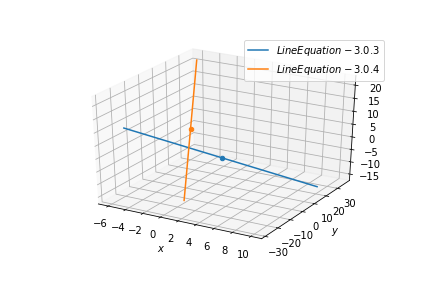
\includegraphics[width=\columnwidth]{./solutions/line_plane/74/codes/figs/Line_interest_1.png}
	\caption{Graph for equations \ref{eq:solutions/line_plane/74/codes7}}
	\label{fig:solutions/line_plane/74/codesline_equation_1}
\end{figure}


	\item 
	\begin{align}\label{eq:solutions/line_plane/74/codes12}
		\frac{x}{2} = \frac{y}{2} &= \frac{z}{1}, 
	\end{align}
	\begin{align}\label{eq:solutions/line_plane/74/codes13}
		\frac{x-5}{4} = \frac{y-2}{1} &= \frac{z-3}{8} 
	\end{align}



The above symmetric equations \ref{eq:solutions/line_plane/74/codes12}, \ref{eq:solutions/line_plane/74/codes13} can be represented in the vector form as 
\begin{align}\label{eq:solutions/line_plane/74/codes14}
	\quad \vec{r_1} &= \myvec{0\\0\\0} + \lambda_1\myvec{2\\2\\1}
	\\
	\quad \vec{r_2} &= \myvec{5\\2\\3} + \lambda_2\myvec{4\\1\\8}
\end{align}

As we have to find the angle between the vectors, we will only be taking the direction vectors into consideration. The direction vectors are $\vec{u}$ = $\myvec{2\\2\\1}$ and $\vec{v}$ = $\myvec{4\\1\\8}$. We can find the corresponding magnitude values

\begin{align}\label{eq:solutions/line_plane/74/codes16}
	\norm{\vec{u}} =\sqrt{2^{2}+2^{2}+1^{2}} =\sqrt{9}
\end{align}
\begin{align}\label{eq:solutions/line_plane/74/codes17}
	\norm{\vec{v}} =\sqrt{4^{2}+1^{2}+8^{2}} =\sqrt{81}
\end{align}

Using \ref{eq:solutions/line_plane/74/codes4}, \ref{eq:solutions/line_plane/74/codes16}, \ref{eq:solutions/line_plane/74/codes17} we get
\begin{align}
	\theta = \cos ^{-1}\frac{\myvec{2\\2\\1}^{T}\myvec{4\\1\\8}}{(\sqrt{9})(\sqrt{81})} 
	\\
	\theta = \cos ^{-1}\frac{18}{27.00}
	\\
	\theta = \cos ^{-1} (0.667)
	\\
	\theta = 48.189\degree
\end{align}

Therefore, the angle between the two lines is $48.189\degree$. See Fig. \ref{fig:solutions/line_plane/74/codesline_equation_2}


\begin{figure}
	\centering
	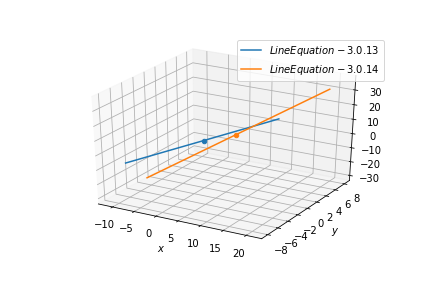
\includegraphics[width=\columnwidth]{./solutions/line_plane/74/codes/figs/Line_interest_2.png}
	\caption{Graph for equations \ref{eq:solutions/line_plane/74/codes14}}
	\label{fig:solutions/line_plane/74/codesline_equation_2}
\end{figure}
\end{enumerate}

    

%
\item    Balance the following chemical equation.
    \begin{align}
        \label{eq:solutions/chem/7b1} \text{Zinc + Silver nitrate} \to \text{Zinc nitrate + Silver}
    \end{align}
\solution
From theory, we understand that using dot product we can find the angle between the lines 
\begin{enumerate}
	\item 
	\begin{align}\label{eq:solutions/line_plane/74/codes:5}
		\frac{x-2}{2} = \frac{y-1}{5} &= \frac{z+3}{-3}, 
	\end{align}
	\begin{align}\label{eq:solutions/line_plane/74/codes:6}
		\frac{x+2}{-1} = \frac{y-4}{8} &= \frac{z-5}{4} 
	\end{align}


The above symmetric equations \ref{eq:solutions/line_plane/74/codes:5}, \ref{eq:solutions/line_plane/74/codes:6} can be represented in the vector form as 
\begin{align}\label{eq:solutions/line_plane/74/codes7}
	\quad \vec{r_1} &= \myvec{2\\1\\-3} + \lambda_1\myvec{2\\5\\-3}
	\\
	\quad \vec{r_2} &= \myvec{-2\\4\\5} + \lambda_2\myvec{-1\\8\\4}
\end{align}

As we have to find the angle between the vectors, we will only be taking the direction vectors into consideration. The direction vectors are $\vec{u}$ = $\myvec{2\\5\\-3}$ and $\vec{v}$ = $\myvec{-1\\8\\4}$. We can find the corresponding magnitude values

\begin{align}\label{eq:solutions/line_plane/74/codes9}
	\norm{\vec{u}} =\sqrt{2^{2}+5^{2}+(-3)^{2}} =\sqrt{38}
\end{align}
\begin{align}\label{eq:solutions/line_plane/74/codes10}
	\norm{\vec{v}} =\sqrt{(-1)^{2}+8^{2}+4^{2}} =\sqrt{81}
\end{align}

Using \ref{eq:solutions/line_plane/74/codes4}, \ref{eq:solutions/line_plane/74/codes9}, \ref{eq:solutions/line_plane/74/codes10} we get
\begin{align}
	\theta = \cos ^{-1}\frac{\myvec{2\\5\\-3}^{T}\myvec{-1\\8\\4}}{(\sqrt{38})(\sqrt{81})} 
	\\
	\theta = \cos ^{-1}\frac{26}{55.4797}
	\\
	\theta = \cos ^{-1} (0.4686)
	\\
	\theta = 62.053\degree
\end{align}

Therefore, the angle between the two lines is $62.053\degree$.See Fig. \ref{fig:solutions/line_plane/74/codesline_equation_1}

\begin{figure}
	\centering
	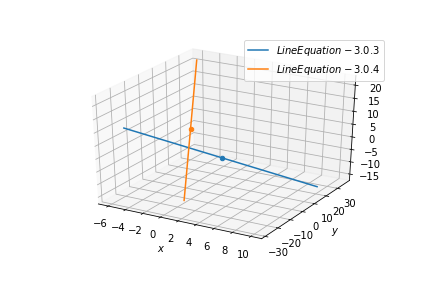
\includegraphics[width=\columnwidth]{./solutions/line_plane/74/codes/figs/Line_interest_1.png}
	\caption{Graph for equations \ref{eq:solutions/line_plane/74/codes7}}
	\label{fig:solutions/line_plane/74/codesline_equation_1}
\end{figure}


	\item 
	\begin{align}\label{eq:solutions/line_plane/74/codes12}
		\frac{x}{2} = \frac{y}{2} &= \frac{z}{1}, 
	\end{align}
	\begin{align}\label{eq:solutions/line_plane/74/codes13}
		\frac{x-5}{4} = \frac{y-2}{1} &= \frac{z-3}{8} 
	\end{align}



The above symmetric equations \ref{eq:solutions/line_plane/74/codes12}, \ref{eq:solutions/line_plane/74/codes13} can be represented in the vector form as 
\begin{align}\label{eq:solutions/line_plane/74/codes14}
	\quad \vec{r_1} &= \myvec{0\\0\\0} + \lambda_1\myvec{2\\2\\1}
	\\
	\quad \vec{r_2} &= \myvec{5\\2\\3} + \lambda_2\myvec{4\\1\\8}
\end{align}

As we have to find the angle between the vectors, we will only be taking the direction vectors into consideration. The direction vectors are $\vec{u}$ = $\myvec{2\\2\\1}$ and $\vec{v}$ = $\myvec{4\\1\\8}$. We can find the corresponding magnitude values

\begin{align}\label{eq:solutions/line_plane/74/codes16}
	\norm{\vec{u}} =\sqrt{2^{2}+2^{2}+1^{2}} =\sqrt{9}
\end{align}
\begin{align}\label{eq:solutions/line_plane/74/codes17}
	\norm{\vec{v}} =\sqrt{4^{2}+1^{2}+8^{2}} =\sqrt{81}
\end{align}

Using \ref{eq:solutions/line_plane/74/codes4}, \ref{eq:solutions/line_plane/74/codes16}, \ref{eq:solutions/line_plane/74/codes17} we get
\begin{align}
	\theta = \cos ^{-1}\frac{\myvec{2\\2\\1}^{T}\myvec{4\\1\\8}}{(\sqrt{9})(\sqrt{81})} 
	\\
	\theta = \cos ^{-1}\frac{18}{27.00}
	\\
	\theta = \cos ^{-1} (0.667)
	\\
	\theta = 48.189\degree
\end{align}

Therefore, the angle between the two lines is $48.189\degree$. See Fig. \ref{fig:solutions/line_plane/74/codesline_equation_2}


\begin{figure}
	\centering
	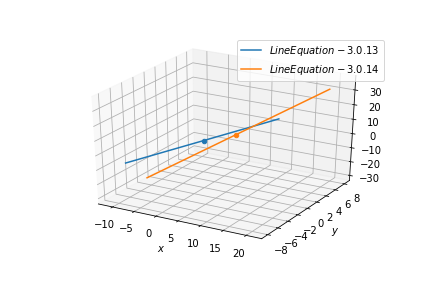
\includegraphics[width=\columnwidth]{./solutions/line_plane/74/codes/figs/Line_interest_2.png}
	\caption{Graph for equations \ref{eq:solutions/line_plane/74/codes14}}
	\label{fig:solutions/line_plane/74/codesline_equation_2}
\end{figure}
\end{enumerate}

    


\item Write the balanced chemical equations for the following reaction :
\begin{align}
 BaCl_2 + K_2SO_4 \rightarrow BaSO_4 + KCl \label{eq:solutions/chemistry/7d:1}   
\end{align}
\solution
From theory, we understand that using dot product we can find the angle between the lines 
\begin{enumerate}
	\item 
	\begin{align}\label{eq:solutions/line_plane/74/codes:5}
		\frac{x-2}{2} = \frac{y-1}{5} &= \frac{z+3}{-3}, 
	\end{align}
	\begin{align}\label{eq:solutions/line_plane/74/codes:6}
		\frac{x+2}{-1} = \frac{y-4}{8} &= \frac{z-5}{4} 
	\end{align}


The above symmetric equations \ref{eq:solutions/line_plane/74/codes:5}, \ref{eq:solutions/line_plane/74/codes:6} can be represented in the vector form as 
\begin{align}\label{eq:solutions/line_plane/74/codes7}
	\quad \vec{r_1} &= \myvec{2\\1\\-3} + \lambda_1\myvec{2\\5\\-3}
	\\
	\quad \vec{r_2} &= \myvec{-2\\4\\5} + \lambda_2\myvec{-1\\8\\4}
\end{align}

As we have to find the angle between the vectors, we will only be taking the direction vectors into consideration. The direction vectors are $\vec{u}$ = $\myvec{2\\5\\-3}$ and $\vec{v}$ = $\myvec{-1\\8\\4}$. We can find the corresponding magnitude values

\begin{align}\label{eq:solutions/line_plane/74/codes9}
	\norm{\vec{u}} =\sqrt{2^{2}+5^{2}+(-3)^{2}} =\sqrt{38}
\end{align}
\begin{align}\label{eq:solutions/line_plane/74/codes10}
	\norm{\vec{v}} =\sqrt{(-1)^{2}+8^{2}+4^{2}} =\sqrt{81}
\end{align}

Using \ref{eq:solutions/line_plane/74/codes4}, \ref{eq:solutions/line_plane/74/codes9}, \ref{eq:solutions/line_plane/74/codes10} we get
\begin{align}
	\theta = \cos ^{-1}\frac{\myvec{2\\5\\-3}^{T}\myvec{-1\\8\\4}}{(\sqrt{38})(\sqrt{81})} 
	\\
	\theta = \cos ^{-1}\frac{26}{55.4797}
	\\
	\theta = \cos ^{-1} (0.4686)
	\\
	\theta = 62.053\degree
\end{align}

Therefore, the angle between the two lines is $62.053\degree$.See Fig. \ref{fig:solutions/line_plane/74/codesline_equation_1}

\begin{figure}
	\centering
	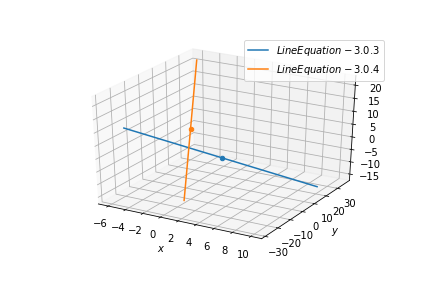
\includegraphics[width=\columnwidth]{./solutions/line_plane/74/codes/figs/Line_interest_1.png}
	\caption{Graph for equations \ref{eq:solutions/line_plane/74/codes7}}
	\label{fig:solutions/line_plane/74/codesline_equation_1}
\end{figure}


	\item 
	\begin{align}\label{eq:solutions/line_plane/74/codes12}
		\frac{x}{2} = \frac{y}{2} &= \frac{z}{1}, 
	\end{align}
	\begin{align}\label{eq:solutions/line_plane/74/codes13}
		\frac{x-5}{4} = \frac{y-2}{1} &= \frac{z-3}{8} 
	\end{align}



The above symmetric equations \ref{eq:solutions/line_plane/74/codes12}, \ref{eq:solutions/line_plane/74/codes13} can be represented in the vector form as 
\begin{align}\label{eq:solutions/line_plane/74/codes14}
	\quad \vec{r_1} &= \myvec{0\\0\\0} + \lambda_1\myvec{2\\2\\1}
	\\
	\quad \vec{r_2} &= \myvec{5\\2\\3} + \lambda_2\myvec{4\\1\\8}
\end{align}

As we have to find the angle between the vectors, we will only be taking the direction vectors into consideration. The direction vectors are $\vec{u}$ = $\myvec{2\\2\\1}$ and $\vec{v}$ = $\myvec{4\\1\\8}$. We can find the corresponding magnitude values

\begin{align}\label{eq:solutions/line_plane/74/codes16}
	\norm{\vec{u}} =\sqrt{2^{2}+2^{2}+1^{2}} =\sqrt{9}
\end{align}
\begin{align}\label{eq:solutions/line_plane/74/codes17}
	\norm{\vec{v}} =\sqrt{4^{2}+1^{2}+8^{2}} =\sqrt{81}
\end{align}

Using \ref{eq:solutions/line_plane/74/codes4}, \ref{eq:solutions/line_plane/74/codes16}, \ref{eq:solutions/line_plane/74/codes17} we get
\begin{align}
	\theta = \cos ^{-1}\frac{\myvec{2\\2\\1}^{T}\myvec{4\\1\\8}}{(\sqrt{9})(\sqrt{81})} 
	\\
	\theta = \cos ^{-1}\frac{18}{27.00}
	\\
	\theta = \cos ^{-1} (0.667)
	\\
	\theta = 48.189\degree
\end{align}

Therefore, the angle between the two lines is $48.189\degree$. See Fig. \ref{fig:solutions/line_plane/74/codesline_equation_2}


\begin{figure}
	\centering
	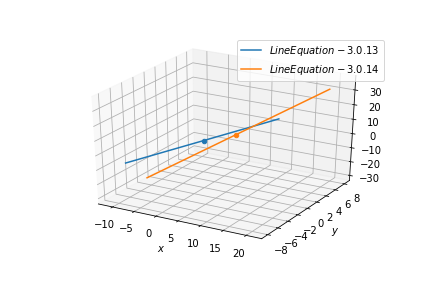
\includegraphics[width=\columnwidth]{./solutions/line_plane/74/codes/figs/Line_interest_2.png}
	\caption{Graph for equations \ref{eq:solutions/line_plane/74/codes14}}
	\label{fig:solutions/line_plane/74/codesline_equation_2}
\end{figure}
\end{enumerate}

    

%

%\end{enumerate}

	
\renewcommand{\theequation}{\theenumi}
\begin{enumerate}[label=\arabic*.,ref=\thesubsection.\theenumi]
\numberwithin{equation}{enumi}

\item Balance the following chemical equation.
%
\begin{align}
\label{eq:chem_balance}
Fe+H_2O &\rightarrow Fe_3O_4 + H_2
\end{align}
%
\solution Let the balanced version of \eqref{eq:chem_balance} be 
%
\begin{align}
\label{eq:chem_balance_unsol}
x_1Fe+x_2H_2 O &\rightarrow x_3Fe_3 O_4 + x_4H_2
\end{align}
%
which results in the following equations
%
\begin{align}
\begin{split}
\brak{x_1 -3x_3}Fe &= 0
\\
\brak{2x_2 -2x_4}H &= 0
\\
\brak{x_2 -4x_3}O &= 0
\end{split}
\end{align}
which can be expressed as
\begin{align}
\begin{split}
x_1 + 0.x_2 -3x_3 +0.x_4&= 0
\\
0.x_1+2x_2 +0.x_3-2x_4 &= 0
\\
0.x_1+x_2 -4x_3+ 0.x_4 &= 0
\end{split}
\end{align}
%
resulting in the matrix equation
\begin{align}
\label{eq:chem_balance_mat_eq}
\begin{split}
\myvec{
1 & 0 & -3 & 0
\\
0 & 2 & 0 & -2
\\
0 & 1 & -4 & 0
}
\vec{x} &= \vec{0}
\end{split}
\end{align}
%
where
\begin{align}
\vec{x} = \myvec{x_1 \\ x_2 \\ x_3 \\ x_4} 
\end{align}
%\item Solve \eqref{eq:chem_balance_unsol} by row reducing 
%the matrix in \eqref{eq:chem_balance_mat_eq}.
%\\
%\solution  
\eqref{eq:chem_balance_mat_eq} can be row reduced as follows
%
\begin{align}
\label{eq:chem_balance_mat_row}
\myvec{
1 & 0 & -3 & 0
\\
0 & 2 & 0 & -2
\\
0 & 1 & -4 & 0
}
 \xleftrightarrow[]{R_2 \leftarrow \frac{R_2}{2}}
\myvec{
1 & 0 & -3 & 0
\\
0 & 1 & 0 & -1
\\
0 & 1 & -4 & 0
}
\\
 \xleftrightarrow[]{R_3\leftarrow R_3-R_2}
\myvec{
1 & 0 & -3 & 0
\\
0 & 1 & 0 & -1
\\
0 & 0 & -4 & 1
}
\\
 \xleftrightarrow[]{R_1\leftarrow 4R_1-3R_3}
\myvec{
4 & 0 & 0 & -3
\\
0 & 1 & 0 & -1
\\
0 & 0 & -4 & 1
}
\\
 \xleftrightarrow[R_3 \leftarrow -\frac{1}{4}R_3]{R_1\leftarrow \frac{1}{4}}
\myvec{
1 & 0 & 0 & -\frac{3}{4}
\\
0 & 1 & 0 & -1
\\
0 & 0 & 1 & -\frac{1}{4}
}
\end{align}
%
Thus, 
\begin{align}
\label{eq:chem_balance_mat_sol}
x_1 &= \frac{3}{4}x_4, x_2 = x_4, x_3 = \frac{1}{4}x_4
\\
\\
\implies 
\vec{x} &= x_4\myvec{\frac{3}{4} \\ 1 \\ \frac{1}{4} \\ 1}= \myvec{3 \\ 4 \\ 1 \\ 4}
\end{align}
%
upon substituting $x_4 = 4$.
%
\eqref{eq:chem_balance_unsol} then becomes
%
\begin{align}
\label{eq:chem_balance_final}
3Fe+4H_2 O &\rightarrow Fe_3 O_4 + 4H_2
\end{align}

\item Consider the following information regarding the number of men and women workers in the three factories I,II and III

\begin{tabular}{ |c|c|c| } 
\hline
 & Men Workers & Women Workers \\
\hline
\multirow{3}{4em}{I \\II \\III} & 30 & 25\\ 
& 25 & 31 \\ 
&27 & 26 \\ 
\hline
\end{tabular}\\
Represent the above information in the form of a 3 $\times$ 2 matrix. What does the entry
in the third row and second column represent?\\


 \item  If a matrix has 8 elements, what are the possible orders it can have?\\
    \item Construct a 3 $\times$ 2 matrix whose elements are given by $a_{ij}=\frac{1}{2}\abs{i-3j}$\\
    \item \myvec{x+3 &z+4 &2y-7\\-6 &a-1 &0\\b-3 &-21 &0}=\myvec{0 &6 &3y-2\\-6 &-3 &2c+2\\2b+4 &-21 &0}\\
    Find the values of a,b,c,x,y and z.\\
\solution 
 As the two matrices are equal their corresponding entries are also equal. Hence
\begin{align}
x+3&=0 \quad \implies x=-3
\\
z+4&=6 \quad \implies z=2
\\
2y-7&=3y-2 \quad \implies y=-5
\\
a-1&=-3 \quad \implies a=-2
\\
2c+2&=0 \quad \implies c=-1
\\
b-3&=2b+4 \quad \implies b=-7
\end{align}

    \item Find the values of a,b,c and d from the following equation:\\
    \myvec{2a+b &a-2b\\5c-d &4c+3d}=\myvec{4 &-3\\11 &24}\\
\solution 
From theory, we understand that using dot product we can find the angle between the lines 
\begin{enumerate}
	\item 
	\begin{align}\label{eq:solutions/line_plane/74/codes:5}
		\frac{x-2}{2} = \frac{y-1}{5} &= \frac{z+3}{-3}, 
	\end{align}
	\begin{align}\label{eq:solutions/line_plane/74/codes:6}
		\frac{x+2}{-1} = \frac{y-4}{8} &= \frac{z-5}{4} 
	\end{align}


The above symmetric equations \ref{eq:solutions/line_plane/74/codes:5}, \ref{eq:solutions/line_plane/74/codes:6} can be represented in the vector form as 
\begin{align}\label{eq:solutions/line_plane/74/codes7}
	\quad \vec{r_1} &= \myvec{2\\1\\-3} + \lambda_1\myvec{2\\5\\-3}
	\\
	\quad \vec{r_2} &= \myvec{-2\\4\\5} + \lambda_2\myvec{-1\\8\\4}
\end{align}

As we have to find the angle between the vectors, we will only be taking the direction vectors into consideration. The direction vectors are $\vec{u}$ = $\myvec{2\\5\\-3}$ and $\vec{v}$ = $\myvec{-1\\8\\4}$. We can find the corresponding magnitude values

\begin{align}\label{eq:solutions/line_plane/74/codes9}
	\norm{\vec{u}} =\sqrt{2^{2}+5^{2}+(-3)^{2}} =\sqrt{38}
\end{align}
\begin{align}\label{eq:solutions/line_plane/74/codes10}
	\norm{\vec{v}} =\sqrt{(-1)^{2}+8^{2}+4^{2}} =\sqrt{81}
\end{align}

Using \ref{eq:solutions/line_plane/74/codes4}, \ref{eq:solutions/line_plane/74/codes9}, \ref{eq:solutions/line_plane/74/codes10} we get
\begin{align}
	\theta = \cos ^{-1}\frac{\myvec{2\\5\\-3}^{T}\myvec{-1\\8\\4}}{(\sqrt{38})(\sqrt{81})} 
	\\
	\theta = \cos ^{-1}\frac{26}{55.4797}
	\\
	\theta = \cos ^{-1} (0.4686)
	\\
	\theta = 62.053\degree
\end{align}

Therefore, the angle between the two lines is $62.053\degree$.See Fig. \ref{fig:solutions/line_plane/74/codesline_equation_1}

\begin{figure}
	\centering
	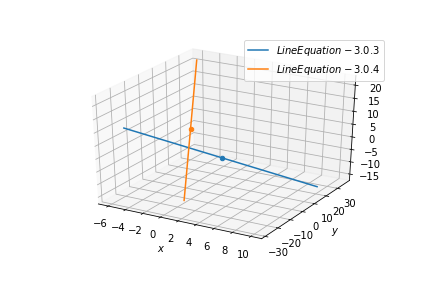
\includegraphics[width=\columnwidth]{./solutions/line_plane/74/codes/figs/Line_interest_1.png}
	\caption{Graph for equations \ref{eq:solutions/line_plane/74/codes7}}
	\label{fig:solutions/line_plane/74/codesline_equation_1}
\end{figure}


	\item 
	\begin{align}\label{eq:solutions/line_plane/74/codes12}
		\frac{x}{2} = \frac{y}{2} &= \frac{z}{1}, 
	\end{align}
	\begin{align}\label{eq:solutions/line_plane/74/codes13}
		\frac{x-5}{4} = \frac{y-2}{1} &= \frac{z-3}{8} 
	\end{align}



The above symmetric equations \ref{eq:solutions/line_plane/74/codes12}, \ref{eq:solutions/line_plane/74/codes13} can be represented in the vector form as 
\begin{align}\label{eq:solutions/line_plane/74/codes14}
	\quad \vec{r_1} &= \myvec{0\\0\\0} + \lambda_1\myvec{2\\2\\1}
	\\
	\quad \vec{r_2} &= \myvec{5\\2\\3} + \lambda_2\myvec{4\\1\\8}
\end{align}

As we have to find the angle between the vectors, we will only be taking the direction vectors into consideration. The direction vectors are $\vec{u}$ = $\myvec{2\\2\\1}$ and $\vec{v}$ = $\myvec{4\\1\\8}$. We can find the corresponding magnitude values

\begin{align}\label{eq:solutions/line_plane/74/codes16}
	\norm{\vec{u}} =\sqrt{2^{2}+2^{2}+1^{2}} =\sqrt{9}
\end{align}
\begin{align}\label{eq:solutions/line_plane/74/codes17}
	\norm{\vec{v}} =\sqrt{4^{2}+1^{2}+8^{2}} =\sqrt{81}
\end{align}

Using \ref{eq:solutions/line_plane/74/codes4}, \ref{eq:solutions/line_plane/74/codes16}, \ref{eq:solutions/line_plane/74/codes17} we get
\begin{align}
	\theta = \cos ^{-1}\frac{\myvec{2\\2\\1}^{T}\myvec{4\\1\\8}}{(\sqrt{9})(\sqrt{81})} 
	\\
	\theta = \cos ^{-1}\frac{18}{27.00}
	\\
	\theta = \cos ^{-1} (0.667)
	\\
	\theta = 48.189\degree
\end{align}

Therefore, the angle between the two lines is $48.189\degree$. See Fig. \ref{fig:solutions/line_plane/74/codesline_equation_2}


\begin{figure}
	\centering
	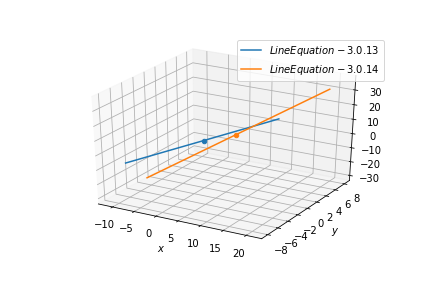
\includegraphics[width=\columnwidth]{./solutions/line_plane/74/codes/figs/Line_interest_2.png}
	\caption{Graph for equations \ref{eq:solutions/line_plane/74/codes14}}
	\label{fig:solutions/line_plane/74/codesline_equation_2}
\end{figure}
\end{enumerate}

    

    \item Given A=\myvec{\sqrt{3} &1 &-1\\2 &3 &0} and B=\myvec{2 &\sqrt{5} &1\\-2 &3 &\frac{1}{2}}, find A+B.\\\solution 
From theory, we understand that using dot product we can find the angle between the lines 
\begin{enumerate}
	\item 
	\begin{align}\label{eq:solutions/line_plane/74/codes:5}
		\frac{x-2}{2} = \frac{y-1}{5} &= \frac{z+3}{-3}, 
	\end{align}
	\begin{align}\label{eq:solutions/line_plane/74/codes:6}
		\frac{x+2}{-1} = \frac{y-4}{8} &= \frac{z-5}{4} 
	\end{align}


The above symmetric equations \ref{eq:solutions/line_plane/74/codes:5}, \ref{eq:solutions/line_plane/74/codes:6} can be represented in the vector form as 
\begin{align}\label{eq:solutions/line_plane/74/codes7}
	\quad \vec{r_1} &= \myvec{2\\1\\-3} + \lambda_1\myvec{2\\5\\-3}
	\\
	\quad \vec{r_2} &= \myvec{-2\\4\\5} + \lambda_2\myvec{-1\\8\\4}
\end{align}

As we have to find the angle between the vectors, we will only be taking the direction vectors into consideration. The direction vectors are $\vec{u}$ = $\myvec{2\\5\\-3}$ and $\vec{v}$ = $\myvec{-1\\8\\4}$. We can find the corresponding magnitude values

\begin{align}\label{eq:solutions/line_plane/74/codes9}
	\norm{\vec{u}} =\sqrt{2^{2}+5^{2}+(-3)^{2}} =\sqrt{38}
\end{align}
\begin{align}\label{eq:solutions/line_plane/74/codes10}
	\norm{\vec{v}} =\sqrt{(-1)^{2}+8^{2}+4^{2}} =\sqrt{81}
\end{align}

Using \ref{eq:solutions/line_plane/74/codes4}, \ref{eq:solutions/line_plane/74/codes9}, \ref{eq:solutions/line_plane/74/codes10} we get
\begin{align}
	\theta = \cos ^{-1}\frac{\myvec{2\\5\\-3}^{T}\myvec{-1\\8\\4}}{(\sqrt{38})(\sqrt{81})} 
	\\
	\theta = \cos ^{-1}\frac{26}{55.4797}
	\\
	\theta = \cos ^{-1} (0.4686)
	\\
	\theta = 62.053\degree
\end{align}

Therefore, the angle between the two lines is $62.053\degree$.See Fig. \ref{fig:solutions/line_plane/74/codesline_equation_1}

\begin{figure}
	\centering
	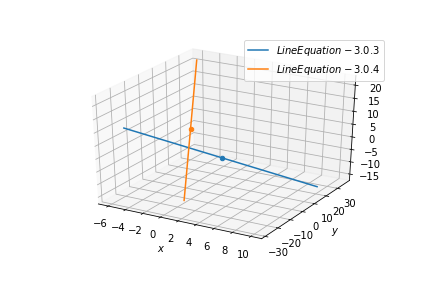
\includegraphics[width=\columnwidth]{./solutions/line_plane/74/codes/figs/Line_interest_1.png}
	\caption{Graph for equations \ref{eq:solutions/line_plane/74/codes7}}
	\label{fig:solutions/line_plane/74/codesline_equation_1}
\end{figure}


	\item 
	\begin{align}\label{eq:solutions/line_plane/74/codes12}
		\frac{x}{2} = \frac{y}{2} &= \frac{z}{1}, 
	\end{align}
	\begin{align}\label{eq:solutions/line_plane/74/codes13}
		\frac{x-5}{4} = \frac{y-2}{1} &= \frac{z-3}{8} 
	\end{align}



The above symmetric equations \ref{eq:solutions/line_plane/74/codes12}, \ref{eq:solutions/line_plane/74/codes13} can be represented in the vector form as 
\begin{align}\label{eq:solutions/line_plane/74/codes14}
	\quad \vec{r_1} &= \myvec{0\\0\\0} + \lambda_1\myvec{2\\2\\1}
	\\
	\quad \vec{r_2} &= \myvec{5\\2\\3} + \lambda_2\myvec{4\\1\\8}
\end{align}

As we have to find the angle between the vectors, we will only be taking the direction vectors into consideration. The direction vectors are $\vec{u}$ = $\myvec{2\\2\\1}$ and $\vec{v}$ = $\myvec{4\\1\\8}$. We can find the corresponding magnitude values

\begin{align}\label{eq:solutions/line_plane/74/codes16}
	\norm{\vec{u}} =\sqrt{2^{2}+2^{2}+1^{2}} =\sqrt{9}
\end{align}
\begin{align}\label{eq:solutions/line_plane/74/codes17}
	\norm{\vec{v}} =\sqrt{4^{2}+1^{2}+8^{2}} =\sqrt{81}
\end{align}

Using \ref{eq:solutions/line_plane/74/codes4}, \ref{eq:solutions/line_plane/74/codes16}, \ref{eq:solutions/line_plane/74/codes17} we get
\begin{align}
	\theta = \cos ^{-1}\frac{\myvec{2\\2\\1}^{T}\myvec{4\\1\\8}}{(\sqrt{9})(\sqrt{81})} 
	\\
	\theta = \cos ^{-1}\frac{18}{27.00}
	\\
	\theta = \cos ^{-1} (0.667)
	\\
	\theta = 48.189\degree
\end{align}

Therefore, the angle between the two lines is $48.189\degree$. See Fig. \ref{fig:solutions/line_plane/74/codesline_equation_2}


\begin{figure}
	\centering
	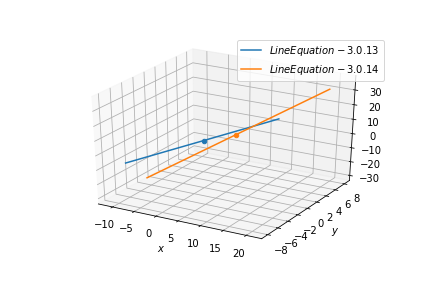
\includegraphics[width=\columnwidth]{./solutions/line_plane/74/codes/figs/Line_interest_2.png}
	\caption{Graph for equations \ref{eq:solutions/line_plane/74/codes14}}
	\label{fig:solutions/line_plane/74/codesline_equation_2}
\end{figure}
\end{enumerate}

    


    \item If A=\myvec{1 &2 &3\\2 &3 &1} and B=\myvec{3 &-1 &3\\-1 &0 &2}, then find 2A-B.\\
    \item If A=\myvec{8 &0\\4 &-2\\3 &6} and B=\myvec{2 &-2\\4 &2\\-5 &1}, then find the matrix X, such that 2A+3X=5B.\\
    \item Find X and Y, if X+Y=\myvec{5 &2\\0 &9} and \\X-Y=\myvec{3 &6\\0 &-1}.\\
    \item Find the values of x and y from the following equation:\\
    2\myvec{x &5\\7 &y-3} + \myvec{3 &-4\\1 &2} = \myvec{7 &6\\15 &14}\\
     
    

    \item Two farmers Ramkishan and Gurcharan Singh cultivates only three
varieties of rice namely Basmati, Permal and Naura. The sale (in Rupees) of these
varieties of rice by both the farmers in the month of September and October are given
by the following matrices A and B. \\
September Sales(in Rupees)\\
   Basmati Permal Naura\\
A =$\myvec{10,000 &20,000 &30,000\\50,000 &30,000 &10,000}$$\myvec{Ramakishan\\Gurucharan Singh}$\\

October sales (in Rupees)\\
  Basmati Permal Naura\\
B=$\myvec{5,000 &10,000 &6,000\\20,000 &10,000 &10,000}$$\myvec{Ramkishan\\Gurucharan Singh}$\\
(i) Find the combined sales in September and October for each farmer in each
variety.\\
(ii) Find the decrease in sales from September to October.\\
(iii) If both farmers receive 2\% profit on gross sales, compute the profit for each
farmer and for each variety sold in October. \\																																															
   
    \item  Find AB, if A=\myvec{6 &9\\2 &3} and B=\myvec{2 &6 &0\\7 &9 &8}.\\
    \item  If A=\myvec{1 &-2 &3\\-4 &2 &5\\} and B=\myvec{2 &3\\4 &5\\2 &1}, then find AB,BA.Show that AB$\neq$BA

   
     \item If A=\myvec{1 &0 \\0 &-1} and  B=\myvec{0 &1\\1 &0}, then find AB,BA. Show that AB$\neq$BA\\
     
   
    \item Find AB, if A=\myvec{0 &-1\\0 &2} and B=\myvec{3 &5\\0 &0}\\
     
   
    \item If A=\myvec{1 &1 &-1\\2 &0 &3\\3 &-1 &2}, B=\myvec{1 &3\\0 &2\\-1 &4} and C=\myvec{1 &2 &3 &-4\\2 &0 &-2 &1}, find\\A(BC),(AB)C and show that (AB)C=A(BC) \\   
    
     \item If A=\myvec{0 &6 &7\\-6 &0 &8\\7 &-8 &0}, B=\myvec{0 &1 &1\\1 &0 &2\\1 &2 &0},C=\myvec{2\\-2\\3}\\Calculate AC,BC and (A+B)C=AC+BC\\

    \item If A=$\myvec{1 &2 &3\\3 &-2 &1\\4 &2 &1}$,then show that $A^3-23A-40I=0$
    
    
    
\item In a legislative assembly election, a political group hired a public relations
firm to promote its candidate in three ways: telephone, house calls, and letters. The
cost per contact (in paise) is given in matrix A as\\ 
Cost per contact\\
A=$\myvec{40 \\100 \\50}\myvec{Telephone \\Housecall \\Letter}$\\
The number of contacts of each type made in two cities X and Y is given by\\
 Telephone  Housecall  Letter\\
B=$\myvec{1000 &500 &5000\\3000 &1000 &10000} \myvec{X \\Y}$. Find the total amount spent by the group in the two cities X and Y. 
\item If A=$\myvec{3 &\sqrt{3} &2\\4 &2 &0}$ and B=$\myvec{2 &-1 &2\\1 &2 &4}$, verify that\\
(i) $(A^{'})^{'}=A$\\ (ii)$(A+B)^{'}=A^{'}+B^{'}$,\\ (iii) $(kB)^{'}=kB^{'}$,where k is any constant.\\
\item If A=$\myvec{-2\\4 \\5}$,B=$\myvec{1 &3 &-6}$, verify that $(AB)^{'}=B^{'}A^{'}$\\
\item Express the matrix B=$\myvec{2 &-2 &-4\\-1 &3 &4\\1 &-2 &-3}$ as the sum of a symmetric and a skew symmetric matrix.\\
\item By using elementary operations,find the inverse of the matrix\\
A=$\myvec{1 &2\\2 &-1}$.\\
\item Obtain the inverse of the following matrix using elementary operations\\
A=$\myvec{0 &1 &2\\1 &2 &3\\3 &1 &1}$.\\
\item Find P$^{-1}$, if it exists, given \\
P=$\myvec{10 &-2\\-5 &1}$.\\
\item If A=$\myvec{\cos\theta &\sin\theta\\ \-sin\theta &\cos\theta}$,\\then prove that $A^{n}=\myvec{\cos\theta &\sin n\theta\\\-sin n\theta &\cos n\theta}$, n $\in$ N.\\
\item If A and B are symmetric matrices of the same order, then show that AB is symmetric if and only if A and B commute,that AB = BA.\\
\item Let A=$\myvec{2 &-1\\3 &4}$, B=$\myvec{5 &2\\7 &4}$, C=$\myvec{2 &5\\3 &8}$. Find a matrix D such that CD-AB=0. 

\end{enumerate}
%\end{document}
    

%\renewcommand{\theequation}{\theenumi}
%\begin{enumerate}[label=\arabic*.,ref=\thesubsection.\theenumi]
%\numberwithin{equation}{enumi}

\item Find 
$\begin{vmatrix}
2&4\\-5&-1
\end{vmatrix}$
\\
\solution 
From theory, we understand that using dot product we can find the angle between the lines 
\begin{enumerate}
	\item 
	\begin{align}\label{eq:solutions/line_plane/74/codes:5}
		\frac{x-2}{2} = \frac{y-1}{5} &= \frac{z+3}{-3}, 
	\end{align}
	\begin{align}\label{eq:solutions/line_plane/74/codes:6}
		\frac{x+2}{-1} = \frac{y-4}{8} &= \frac{z-5}{4} 
	\end{align}


The above symmetric equations \ref{eq:solutions/line_plane/74/codes:5}, \ref{eq:solutions/line_plane/74/codes:6} can be represented in the vector form as 
\begin{align}\label{eq:solutions/line_plane/74/codes7}
	\quad \vec{r_1} &= \myvec{2\\1\\-3} + \lambda_1\myvec{2\\5\\-3}
	\\
	\quad \vec{r_2} &= \myvec{-2\\4\\5} + \lambda_2\myvec{-1\\8\\4}
\end{align}

As we have to find the angle between the vectors, we will only be taking the direction vectors into consideration. The direction vectors are $\vec{u}$ = $\myvec{2\\5\\-3}$ and $\vec{v}$ = $\myvec{-1\\8\\4}$. We can find the corresponding magnitude values

\begin{align}\label{eq:solutions/line_plane/74/codes9}
	\norm{\vec{u}} =\sqrt{2^{2}+5^{2}+(-3)^{2}} =\sqrt{38}
\end{align}
\begin{align}\label{eq:solutions/line_plane/74/codes10}
	\norm{\vec{v}} =\sqrt{(-1)^{2}+8^{2}+4^{2}} =\sqrt{81}
\end{align}

Using \ref{eq:solutions/line_plane/74/codes4}, \ref{eq:solutions/line_plane/74/codes9}, \ref{eq:solutions/line_plane/74/codes10} we get
\begin{align}
	\theta = \cos ^{-1}\frac{\myvec{2\\5\\-3}^{T}\myvec{-1\\8\\4}}{(\sqrt{38})(\sqrt{81})} 
	\\
	\theta = \cos ^{-1}\frac{26}{55.4797}
	\\
	\theta = \cos ^{-1} (0.4686)
	\\
	\theta = 62.053\degree
\end{align}

Therefore, the angle between the two lines is $62.053\degree$.See Fig. \ref{fig:solutions/line_plane/74/codesline_equation_1}

\begin{figure}
	\centering
	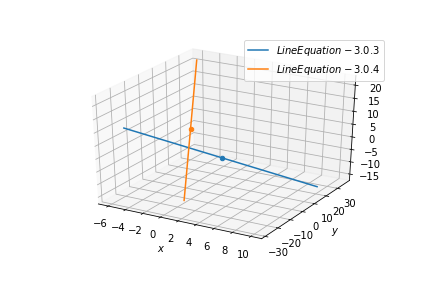
\includegraphics[width=\columnwidth]{./solutions/line_plane/74/codes/figs/Line_interest_1.png}
	\caption{Graph for equations \ref{eq:solutions/line_plane/74/codes7}}
	\label{fig:solutions/line_plane/74/codesline_equation_1}
\end{figure}


	\item 
	\begin{align}\label{eq:solutions/line_plane/74/codes12}
		\frac{x}{2} = \frac{y}{2} &= \frac{z}{1}, 
	\end{align}
	\begin{align}\label{eq:solutions/line_plane/74/codes13}
		\frac{x-5}{4} = \frac{y-2}{1} &= \frac{z-3}{8} 
	\end{align}



The above symmetric equations \ref{eq:solutions/line_plane/74/codes12}, \ref{eq:solutions/line_plane/74/codes13} can be represented in the vector form as 
\begin{align}\label{eq:solutions/line_plane/74/codes14}
	\quad \vec{r_1} &= \myvec{0\\0\\0} + \lambda_1\myvec{2\\2\\1}
	\\
	\quad \vec{r_2} &= \myvec{5\\2\\3} + \lambda_2\myvec{4\\1\\8}
\end{align}

As we have to find the angle between the vectors, we will only be taking the direction vectors into consideration. The direction vectors are $\vec{u}$ = $\myvec{2\\2\\1}$ and $\vec{v}$ = $\myvec{4\\1\\8}$. We can find the corresponding magnitude values

\begin{align}\label{eq:solutions/line_plane/74/codes16}
	\norm{\vec{u}} =\sqrt{2^{2}+2^{2}+1^{2}} =\sqrt{9}
\end{align}
\begin{align}\label{eq:solutions/line_plane/74/codes17}
	\norm{\vec{v}} =\sqrt{4^{2}+1^{2}+8^{2}} =\sqrt{81}
\end{align}

Using \ref{eq:solutions/line_plane/74/codes4}, \ref{eq:solutions/line_plane/74/codes16}, \ref{eq:solutions/line_plane/74/codes17} we get
\begin{align}
	\theta = \cos ^{-1}\frac{\myvec{2\\2\\1}^{T}\myvec{4\\1\\8}}{(\sqrt{9})(\sqrt{81})} 
	\\
	\theta = \cos ^{-1}\frac{18}{27.00}
	\\
	\theta = \cos ^{-1} (0.667)
	\\
	\theta = 48.189\degree
\end{align}

Therefore, the angle between the two lines is $48.189\degree$. See Fig. \ref{fig:solutions/line_plane/74/codesline_equation_2}


\begin{figure}
	\centering
	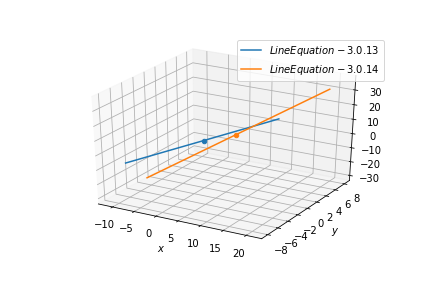
\includegraphics[width=\columnwidth]{./solutions/line_plane/74/codes/figs/Line_interest_2.png}
	\caption{Graph for equations \ref{eq:solutions/line_plane/74/codes14}}
	\label{fig:solutions/line_plane/74/codesline_equation_2}
\end{figure}
\end{enumerate}

    


\item (i) $\begin{vmatrix}\cos\theta& -\sin\theta\\ \sin\theta& \cos\theta \end{vmatrix}$ 
(ii) $\begin{vmatrix}
x^2-x+1& x-1\\ x+1&  x+1
\end{vmatrix}$
\\
\solution 
From theory, we understand that using dot product we can find the angle between the lines 
\begin{enumerate}
	\item 
	\begin{align}\label{eq:solutions/line_plane/74/codes:5}
		\frac{x-2}{2} = \frac{y-1}{5} &= \frac{z+3}{-3}, 
	\end{align}
	\begin{align}\label{eq:solutions/line_plane/74/codes:6}
		\frac{x+2}{-1} = \frac{y-4}{8} &= \frac{z-5}{4} 
	\end{align}


The above symmetric equations \ref{eq:solutions/line_plane/74/codes:5}, \ref{eq:solutions/line_plane/74/codes:6} can be represented in the vector form as 
\begin{align}\label{eq:solutions/line_plane/74/codes7}
	\quad \vec{r_1} &= \myvec{2\\1\\-3} + \lambda_1\myvec{2\\5\\-3}
	\\
	\quad \vec{r_2} &= \myvec{-2\\4\\5} + \lambda_2\myvec{-1\\8\\4}
\end{align}

As we have to find the angle between the vectors, we will only be taking the direction vectors into consideration. The direction vectors are $\vec{u}$ = $\myvec{2\\5\\-3}$ and $\vec{v}$ = $\myvec{-1\\8\\4}$. We can find the corresponding magnitude values

\begin{align}\label{eq:solutions/line_plane/74/codes9}
	\norm{\vec{u}} =\sqrt{2^{2}+5^{2}+(-3)^{2}} =\sqrt{38}
\end{align}
\begin{align}\label{eq:solutions/line_plane/74/codes10}
	\norm{\vec{v}} =\sqrt{(-1)^{2}+8^{2}+4^{2}} =\sqrt{81}
\end{align}

Using \ref{eq:solutions/line_plane/74/codes4}, \ref{eq:solutions/line_plane/74/codes9}, \ref{eq:solutions/line_plane/74/codes10} we get
\begin{align}
	\theta = \cos ^{-1}\frac{\myvec{2\\5\\-3}^{T}\myvec{-1\\8\\4}}{(\sqrt{38})(\sqrt{81})} 
	\\
	\theta = \cos ^{-1}\frac{26}{55.4797}
	\\
	\theta = \cos ^{-1} (0.4686)
	\\
	\theta = 62.053\degree
\end{align}

Therefore, the angle between the two lines is $62.053\degree$.See Fig. \ref{fig:solutions/line_plane/74/codesline_equation_1}

\begin{figure}
	\centering
	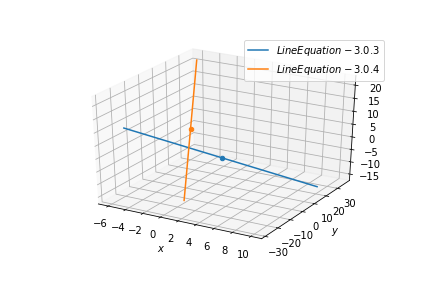
\includegraphics[width=\columnwidth]{./solutions/line_plane/74/codes/figs/Line_interest_1.png}
	\caption{Graph for equations \ref{eq:solutions/line_plane/74/codes7}}
	\label{fig:solutions/line_plane/74/codesline_equation_1}
\end{figure}


	\item 
	\begin{align}\label{eq:solutions/line_plane/74/codes12}
		\frac{x}{2} = \frac{y}{2} &= \frac{z}{1}, 
	\end{align}
	\begin{align}\label{eq:solutions/line_plane/74/codes13}
		\frac{x-5}{4} = \frac{y-2}{1} &= \frac{z-3}{8} 
	\end{align}



The above symmetric equations \ref{eq:solutions/line_plane/74/codes12}, \ref{eq:solutions/line_plane/74/codes13} can be represented in the vector form as 
\begin{align}\label{eq:solutions/line_plane/74/codes14}
	\quad \vec{r_1} &= \myvec{0\\0\\0} + \lambda_1\myvec{2\\2\\1}
	\\
	\quad \vec{r_2} &= \myvec{5\\2\\3} + \lambda_2\myvec{4\\1\\8}
\end{align}

As we have to find the angle between the vectors, we will only be taking the direction vectors into consideration. The direction vectors are $\vec{u}$ = $\myvec{2\\2\\1}$ and $\vec{v}$ = $\myvec{4\\1\\8}$. We can find the corresponding magnitude values

\begin{align}\label{eq:solutions/line_plane/74/codes16}
	\norm{\vec{u}} =\sqrt{2^{2}+2^{2}+1^{2}} =\sqrt{9}
\end{align}
\begin{align}\label{eq:solutions/line_plane/74/codes17}
	\norm{\vec{v}} =\sqrt{4^{2}+1^{2}+8^{2}} =\sqrt{81}
\end{align}

Using \ref{eq:solutions/line_plane/74/codes4}, \ref{eq:solutions/line_plane/74/codes16}, \ref{eq:solutions/line_plane/74/codes17} we get
\begin{align}
	\theta = \cos ^{-1}\frac{\myvec{2\\2\\1}^{T}\myvec{4\\1\\8}}{(\sqrt{9})(\sqrt{81})} 
	\\
	\theta = \cos ^{-1}\frac{18}{27.00}
	\\
	\theta = \cos ^{-1} (0.667)
	\\
	\theta = 48.189\degree
\end{align}

Therefore, the angle between the two lines is $48.189\degree$. See Fig. \ref{fig:solutions/line_plane/74/codesline_equation_2}


\begin{figure}
	\centering
	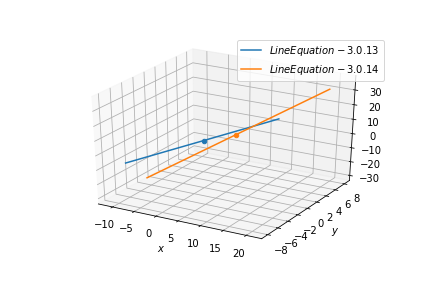
\includegraphics[width=\columnwidth]{./solutions/line_plane/74/codes/figs/Line_interest_2.png}
	\caption{Graph for equations \ref{eq:solutions/line_plane/74/codes14}}
	\label{fig:solutions/line_plane/74/codesline_equation_2}
\end{figure}
\end{enumerate}

    

\item If$ \vec{A} = \begin{vmatrix}1&2\\4&2\end{vmatrix}$,then show that  
$\abs{2\vec{A}}=4\abs{\vec{A}}$
\\
\solution 
From theory, we understand that using dot product we can find the angle between the lines 
\begin{enumerate}
	\item 
	\begin{align}\label{eq:solutions/line_plane/74/codes:5}
		\frac{x-2}{2} = \frac{y-1}{5} &= \frac{z+3}{-3}, 
	\end{align}
	\begin{align}\label{eq:solutions/line_plane/74/codes:6}
		\frac{x+2}{-1} = \frac{y-4}{8} &= \frac{z-5}{4} 
	\end{align}


The above symmetric equations \ref{eq:solutions/line_plane/74/codes:5}, \ref{eq:solutions/line_plane/74/codes:6} can be represented in the vector form as 
\begin{align}\label{eq:solutions/line_plane/74/codes7}
	\quad \vec{r_1} &= \myvec{2\\1\\-3} + \lambda_1\myvec{2\\5\\-3}
	\\
	\quad \vec{r_2} &= \myvec{-2\\4\\5} + \lambda_2\myvec{-1\\8\\4}
\end{align}

As we have to find the angle between the vectors, we will only be taking the direction vectors into consideration. The direction vectors are $\vec{u}$ = $\myvec{2\\5\\-3}$ and $\vec{v}$ = $\myvec{-1\\8\\4}$. We can find the corresponding magnitude values

\begin{align}\label{eq:solutions/line_plane/74/codes9}
	\norm{\vec{u}} =\sqrt{2^{2}+5^{2}+(-3)^{2}} =\sqrt{38}
\end{align}
\begin{align}\label{eq:solutions/line_plane/74/codes10}
	\norm{\vec{v}} =\sqrt{(-1)^{2}+8^{2}+4^{2}} =\sqrt{81}
\end{align}

Using \ref{eq:solutions/line_plane/74/codes4}, \ref{eq:solutions/line_plane/74/codes9}, \ref{eq:solutions/line_plane/74/codes10} we get
\begin{align}
	\theta = \cos ^{-1}\frac{\myvec{2\\5\\-3}^{T}\myvec{-1\\8\\4}}{(\sqrt{38})(\sqrt{81})} 
	\\
	\theta = \cos ^{-1}\frac{26}{55.4797}
	\\
	\theta = \cos ^{-1} (0.4686)
	\\
	\theta = 62.053\degree
\end{align}

Therefore, the angle between the two lines is $62.053\degree$.See Fig. \ref{fig:solutions/line_plane/74/codesline_equation_1}

\begin{figure}
	\centering
	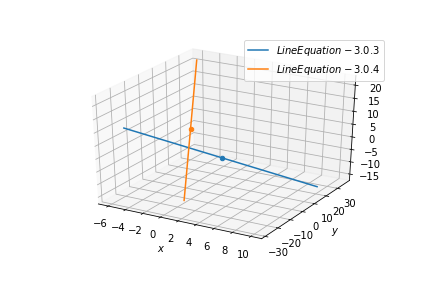
\includegraphics[width=\columnwidth]{./solutions/line_plane/74/codes/figs/Line_interest_1.png}
	\caption{Graph for equations \ref{eq:solutions/line_plane/74/codes7}}
	\label{fig:solutions/line_plane/74/codesline_equation_1}
\end{figure}


	\item 
	\begin{align}\label{eq:solutions/line_plane/74/codes12}
		\frac{x}{2} = \frac{y}{2} &= \frac{z}{1}, 
	\end{align}
	\begin{align}\label{eq:solutions/line_plane/74/codes13}
		\frac{x-5}{4} = \frac{y-2}{1} &= \frac{z-3}{8} 
	\end{align}



The above symmetric equations \ref{eq:solutions/line_plane/74/codes12}, \ref{eq:solutions/line_plane/74/codes13} can be represented in the vector form as 
\begin{align}\label{eq:solutions/line_plane/74/codes14}
	\quad \vec{r_1} &= \myvec{0\\0\\0} + \lambda_1\myvec{2\\2\\1}
	\\
	\quad \vec{r_2} &= \myvec{5\\2\\3} + \lambda_2\myvec{4\\1\\8}
\end{align}

As we have to find the angle between the vectors, we will only be taking the direction vectors into consideration. The direction vectors are $\vec{u}$ = $\myvec{2\\2\\1}$ and $\vec{v}$ = $\myvec{4\\1\\8}$. We can find the corresponding magnitude values

\begin{align}\label{eq:solutions/line_plane/74/codes16}
	\norm{\vec{u}} =\sqrt{2^{2}+2^{2}+1^{2}} =\sqrt{9}
\end{align}
\begin{align}\label{eq:solutions/line_plane/74/codes17}
	\norm{\vec{v}} =\sqrt{4^{2}+1^{2}+8^{2}} =\sqrt{81}
\end{align}

Using \ref{eq:solutions/line_plane/74/codes4}, \ref{eq:solutions/line_plane/74/codes16}, \ref{eq:solutions/line_plane/74/codes17} we get
\begin{align}
	\theta = \cos ^{-1}\frac{\myvec{2\\2\\1}^{T}\myvec{4\\1\\8}}{(\sqrt{9})(\sqrt{81})} 
	\\
	\theta = \cos ^{-1}\frac{18}{27.00}
	\\
	\theta = \cos ^{-1} (0.667)
	\\
	\theta = 48.189\degree
\end{align}

Therefore, the angle between the two lines is $48.189\degree$. See Fig. \ref{fig:solutions/line_plane/74/codesline_equation_2}


\begin{figure}
	\centering
	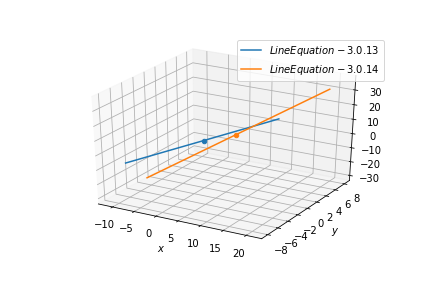
\includegraphics[width=\columnwidth]{./solutions/line_plane/74/codes/figs/Line_interest_2.png}
	\caption{Graph for equations \ref{eq:solutions/line_plane/74/codes14}}
	\label{fig:solutions/line_plane/74/codesline_equation_2}
\end{figure}
\end{enumerate}

    

\item If $\vec{A}=\begin{vmatrix}1&0&1\\0&1&2\\0&0&4\end{vmatrix}$, then show that $\abs{3\vec{A}}=27\abs{\vec{A}}$
\\
\solution 
From theory, we understand that using dot product we can find the angle between the lines 
\begin{enumerate}
	\item 
	\begin{align}\label{eq:solutions/line_plane/74/codes:5}
		\frac{x-2}{2} = \frac{y-1}{5} &= \frac{z+3}{-3}, 
	\end{align}
	\begin{align}\label{eq:solutions/line_plane/74/codes:6}
		\frac{x+2}{-1} = \frac{y-4}{8} &= \frac{z-5}{4} 
	\end{align}


The above symmetric equations \ref{eq:solutions/line_plane/74/codes:5}, \ref{eq:solutions/line_plane/74/codes:6} can be represented in the vector form as 
\begin{align}\label{eq:solutions/line_plane/74/codes7}
	\quad \vec{r_1} &= \myvec{2\\1\\-3} + \lambda_1\myvec{2\\5\\-3}
	\\
	\quad \vec{r_2} &= \myvec{-2\\4\\5} + \lambda_2\myvec{-1\\8\\4}
\end{align}

As we have to find the angle between the vectors, we will only be taking the direction vectors into consideration. The direction vectors are $\vec{u}$ = $\myvec{2\\5\\-3}$ and $\vec{v}$ = $\myvec{-1\\8\\4}$. We can find the corresponding magnitude values

\begin{align}\label{eq:solutions/line_plane/74/codes9}
	\norm{\vec{u}} =\sqrt{2^{2}+5^{2}+(-3)^{2}} =\sqrt{38}
\end{align}
\begin{align}\label{eq:solutions/line_plane/74/codes10}
	\norm{\vec{v}} =\sqrt{(-1)^{2}+8^{2}+4^{2}} =\sqrt{81}
\end{align}

Using \ref{eq:solutions/line_plane/74/codes4}, \ref{eq:solutions/line_plane/74/codes9}, \ref{eq:solutions/line_plane/74/codes10} we get
\begin{align}
	\theta = \cos ^{-1}\frac{\myvec{2\\5\\-3}^{T}\myvec{-1\\8\\4}}{(\sqrt{38})(\sqrt{81})} 
	\\
	\theta = \cos ^{-1}\frac{26}{55.4797}
	\\
	\theta = \cos ^{-1} (0.4686)
	\\
	\theta = 62.053\degree
\end{align}

Therefore, the angle between the two lines is $62.053\degree$.See Fig. \ref{fig:solutions/line_plane/74/codesline_equation_1}

\begin{figure}
	\centering
	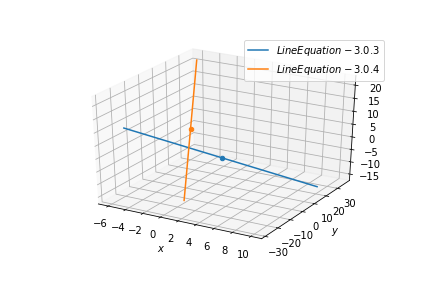
\includegraphics[width=\columnwidth]{./solutions/line_plane/74/codes/figs/Line_interest_1.png}
	\caption{Graph for equations \ref{eq:solutions/line_plane/74/codes7}}
	\label{fig:solutions/line_plane/74/codesline_equation_1}
\end{figure}


	\item 
	\begin{align}\label{eq:solutions/line_plane/74/codes12}
		\frac{x}{2} = \frac{y}{2} &= \frac{z}{1}, 
	\end{align}
	\begin{align}\label{eq:solutions/line_plane/74/codes13}
		\frac{x-5}{4} = \frac{y-2}{1} &= \frac{z-3}{8} 
	\end{align}



The above symmetric equations \ref{eq:solutions/line_plane/74/codes12}, \ref{eq:solutions/line_plane/74/codes13} can be represented in the vector form as 
\begin{align}\label{eq:solutions/line_plane/74/codes14}
	\quad \vec{r_1} &= \myvec{0\\0\\0} + \lambda_1\myvec{2\\2\\1}
	\\
	\quad \vec{r_2} &= \myvec{5\\2\\3} + \lambda_2\myvec{4\\1\\8}
\end{align}

As we have to find the angle between the vectors, we will only be taking the direction vectors into consideration. The direction vectors are $\vec{u}$ = $\myvec{2\\2\\1}$ and $\vec{v}$ = $\myvec{4\\1\\8}$. We can find the corresponding magnitude values

\begin{align}\label{eq:solutions/line_plane/74/codes16}
	\norm{\vec{u}} =\sqrt{2^{2}+2^{2}+1^{2}} =\sqrt{9}
\end{align}
\begin{align}\label{eq:solutions/line_plane/74/codes17}
	\norm{\vec{v}} =\sqrt{4^{2}+1^{2}+8^{2}} =\sqrt{81}
\end{align}

Using \ref{eq:solutions/line_plane/74/codes4}, \ref{eq:solutions/line_plane/74/codes16}, \ref{eq:solutions/line_plane/74/codes17} we get
\begin{align}
	\theta = \cos ^{-1}\frac{\myvec{2\\2\\1}^{T}\myvec{4\\1\\8}}{(\sqrt{9})(\sqrt{81})} 
	\\
	\theta = \cos ^{-1}\frac{18}{27.00}
	\\
	\theta = \cos ^{-1} (0.667)
	\\
	\theta = 48.189\degree
\end{align}

Therefore, the angle between the two lines is $48.189\degree$. See Fig. \ref{fig:solutions/line_plane/74/codesline_equation_2}


\begin{figure}
	\centering
	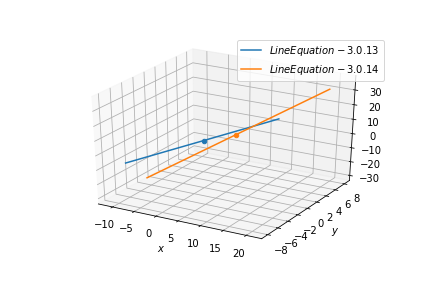
\includegraphics[width=\columnwidth]{./solutions/line_plane/74/codes/figs/Line_interest_2.png}
	\caption{Graph for equations \ref{eq:solutions/line_plane/74/codes14}}
	\label{fig:solutions/line_plane/74/codesline_equation_2}
\end{figure}
\end{enumerate}

    

\item Evaluate the determinants
\begin{enumerate}
\item $\begin{vmatrix}
3&-1&-2\\0&0&-1\\3&-5&0
\end{vmatrix}$
\item $\begin{vmatrix}
3&-4&5\\1&1&-2\\2&3&1
\end{vmatrix}$
\\
\solution 

The following python code computes the required determinant value.
	\begin{lstlisting}
	./solutions/5/codes/lines/q14.py
	\end{lstlisting}
	
	\begin{enumerate}
		\item $\mydet{3&-1&-2\\0&0&-1\\3&-5&0} = -12$
		\item $\mydet{3&-4&5\\1&1&-2\\2&3&1} = -46$
		\item $\mydet{0&1&2\\-1&0&-3\\-2&3&0}=0$
		\item $\mydet{2&-1&-2\\0&2&-1\\3&-5&0} = 5$

	\end{enumerate}

\item $\begin{vmatrix}
0&1&2 \\ -1&0&-3\\-2&3&0
\end{vmatrix}$
\item $\begin{vmatrix}
2&-1&-2\\0&2&-1\\3&-5&0
\end{vmatrix}$
\end{enumerate}  
\item If A=$\begin{vmatrix}1&1&-2\\2&1&-3\\5&4&-9\end{vmatrix}$, 
find $\abs{A}$
\\
\solution 
From theory, we understand that using dot product we can find the angle between the lines 
\begin{enumerate}
	\item 
	\begin{align}\label{eq:solutions/line_plane/74/codes:5}
		\frac{x-2}{2} = \frac{y-1}{5} &= \frac{z+3}{-3}, 
	\end{align}
	\begin{align}\label{eq:solutions/line_plane/74/codes:6}
		\frac{x+2}{-1} = \frac{y-4}{8} &= \frac{z-5}{4} 
	\end{align}


The above symmetric equations \ref{eq:solutions/line_plane/74/codes:5}, \ref{eq:solutions/line_plane/74/codes:6} can be represented in the vector form as 
\begin{align}\label{eq:solutions/line_plane/74/codes7}
	\quad \vec{r_1} &= \myvec{2\\1\\-3} + \lambda_1\myvec{2\\5\\-3}
	\\
	\quad \vec{r_2} &= \myvec{-2\\4\\5} + \lambda_2\myvec{-1\\8\\4}
\end{align}

As we have to find the angle between the vectors, we will only be taking the direction vectors into consideration. The direction vectors are $\vec{u}$ = $\myvec{2\\5\\-3}$ and $\vec{v}$ = $\myvec{-1\\8\\4}$. We can find the corresponding magnitude values

\begin{align}\label{eq:solutions/line_plane/74/codes9}
	\norm{\vec{u}} =\sqrt{2^{2}+5^{2}+(-3)^{2}} =\sqrt{38}
\end{align}
\begin{align}\label{eq:solutions/line_plane/74/codes10}
	\norm{\vec{v}} =\sqrt{(-1)^{2}+8^{2}+4^{2}} =\sqrt{81}
\end{align}

Using \ref{eq:solutions/line_plane/74/codes4}, \ref{eq:solutions/line_plane/74/codes9}, \ref{eq:solutions/line_plane/74/codes10} we get
\begin{align}
	\theta = \cos ^{-1}\frac{\myvec{2\\5\\-3}^{T}\myvec{-1\\8\\4}}{(\sqrt{38})(\sqrt{81})} 
	\\
	\theta = \cos ^{-1}\frac{26}{55.4797}
	\\
	\theta = \cos ^{-1} (0.4686)
	\\
	\theta = 62.053\degree
\end{align}

Therefore, the angle between the two lines is $62.053\degree$.See Fig. \ref{fig:solutions/line_plane/74/codesline_equation_1}

\begin{figure}
	\centering
	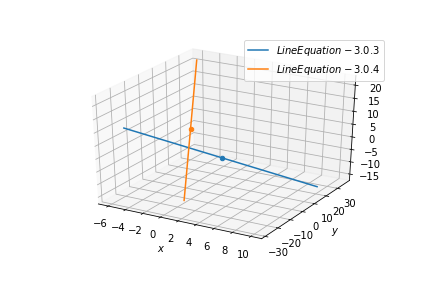
\includegraphics[width=\columnwidth]{./solutions/line_plane/74/codes/figs/Line_interest_1.png}
	\caption{Graph for equations \ref{eq:solutions/line_plane/74/codes7}}
	\label{fig:solutions/line_plane/74/codesline_equation_1}
\end{figure}


	\item 
	\begin{align}\label{eq:solutions/line_plane/74/codes12}
		\frac{x}{2} = \frac{y}{2} &= \frac{z}{1}, 
	\end{align}
	\begin{align}\label{eq:solutions/line_plane/74/codes13}
		\frac{x-5}{4} = \frac{y-2}{1} &= \frac{z-3}{8} 
	\end{align}



The above symmetric equations \ref{eq:solutions/line_plane/74/codes12}, \ref{eq:solutions/line_plane/74/codes13} can be represented in the vector form as 
\begin{align}\label{eq:solutions/line_plane/74/codes14}
	\quad \vec{r_1} &= \myvec{0\\0\\0} + \lambda_1\myvec{2\\2\\1}
	\\
	\quad \vec{r_2} &= \myvec{5\\2\\3} + \lambda_2\myvec{4\\1\\8}
\end{align}

As we have to find the angle between the vectors, we will only be taking the direction vectors into consideration. The direction vectors are $\vec{u}$ = $\myvec{2\\2\\1}$ and $\vec{v}$ = $\myvec{4\\1\\8}$. We can find the corresponding magnitude values

\begin{align}\label{eq:solutions/line_plane/74/codes16}
	\norm{\vec{u}} =\sqrt{2^{2}+2^{2}+1^{2}} =\sqrt{9}
\end{align}
\begin{align}\label{eq:solutions/line_plane/74/codes17}
	\norm{\vec{v}} =\sqrt{4^{2}+1^{2}+8^{2}} =\sqrt{81}
\end{align}

Using \ref{eq:solutions/line_plane/74/codes4}, \ref{eq:solutions/line_plane/74/codes16}, \ref{eq:solutions/line_plane/74/codes17} we get
\begin{align}
	\theta = \cos ^{-1}\frac{\myvec{2\\2\\1}^{T}\myvec{4\\1\\8}}{(\sqrt{9})(\sqrt{81})} 
	\\
	\theta = \cos ^{-1}\frac{18}{27.00}
	\\
	\theta = \cos ^{-1} (0.667)
	\\
	\theta = 48.189\degree
\end{align}

Therefore, the angle between the two lines is $48.189\degree$. See Fig. \ref{fig:solutions/line_plane/74/codesline_equation_2}


\begin{figure}
	\centering
	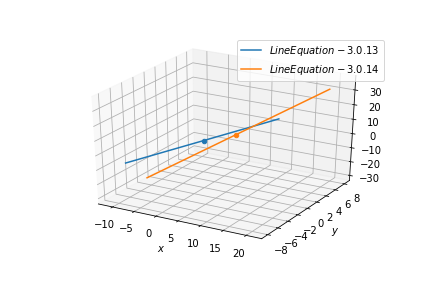
\includegraphics[width=\columnwidth]{./solutions/line_plane/74/codes/figs/Line_interest_2.png}
	\caption{Graph for equations \ref{eq:solutions/line_plane/74/codes14}}
	\label{fig:solutions/line_plane/74/codesline_equation_2}
\end{figure}
\end{enumerate}

    

\item Find the values of x,If\\
(i)$\begin{vmatrix}
2&4\\5&1
\end{vmatrix}$ =$\begin{vmatrix}
2x&4 \\ 6&x
\end{vmatrix}$
(ii)$\begin{vmatrix}
2&3 \\ 4&5
\end{vmatrix}$ =$\begin{vmatrix}
x&3 \\ 2x&5
\end{vmatrix}$
\\
\solution 
From theory, we understand that using dot product we can find the angle between the lines 
\begin{enumerate}
	\item 
	\begin{align}\label{eq:solutions/line_plane/74/codes:5}
		\frac{x-2}{2} = \frac{y-1}{5} &= \frac{z+3}{-3}, 
	\end{align}
	\begin{align}\label{eq:solutions/line_plane/74/codes:6}
		\frac{x+2}{-1} = \frac{y-4}{8} &= \frac{z-5}{4} 
	\end{align}


The above symmetric equations \ref{eq:solutions/line_plane/74/codes:5}, \ref{eq:solutions/line_plane/74/codes:6} can be represented in the vector form as 
\begin{align}\label{eq:solutions/line_plane/74/codes7}
	\quad \vec{r_1} &= \myvec{2\\1\\-3} + \lambda_1\myvec{2\\5\\-3}
	\\
	\quad \vec{r_2} &= \myvec{-2\\4\\5} + \lambda_2\myvec{-1\\8\\4}
\end{align}

As we have to find the angle between the vectors, we will only be taking the direction vectors into consideration. The direction vectors are $\vec{u}$ = $\myvec{2\\5\\-3}$ and $\vec{v}$ = $\myvec{-1\\8\\4}$. We can find the corresponding magnitude values

\begin{align}\label{eq:solutions/line_plane/74/codes9}
	\norm{\vec{u}} =\sqrt{2^{2}+5^{2}+(-3)^{2}} =\sqrt{38}
\end{align}
\begin{align}\label{eq:solutions/line_plane/74/codes10}
	\norm{\vec{v}} =\sqrt{(-1)^{2}+8^{2}+4^{2}} =\sqrt{81}
\end{align}

Using \ref{eq:solutions/line_plane/74/codes4}, \ref{eq:solutions/line_plane/74/codes9}, \ref{eq:solutions/line_plane/74/codes10} we get
\begin{align}
	\theta = \cos ^{-1}\frac{\myvec{2\\5\\-3}^{T}\myvec{-1\\8\\4}}{(\sqrt{38})(\sqrt{81})} 
	\\
	\theta = \cos ^{-1}\frac{26}{55.4797}
	\\
	\theta = \cos ^{-1} (0.4686)
	\\
	\theta = 62.053\degree
\end{align}

Therefore, the angle between the two lines is $62.053\degree$.See Fig. \ref{fig:solutions/line_plane/74/codesline_equation_1}

\begin{figure}
	\centering
	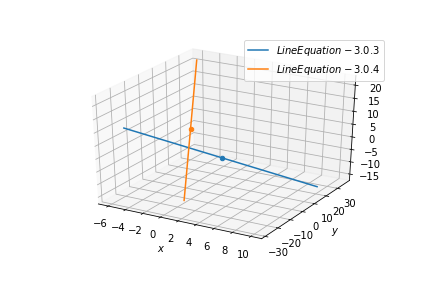
\includegraphics[width=\columnwidth]{./solutions/line_plane/74/codes/figs/Line_interest_1.png}
	\caption{Graph for equations \ref{eq:solutions/line_plane/74/codes7}}
	\label{fig:solutions/line_plane/74/codesline_equation_1}
\end{figure}


	\item 
	\begin{align}\label{eq:solutions/line_plane/74/codes12}
		\frac{x}{2} = \frac{y}{2} &= \frac{z}{1}, 
	\end{align}
	\begin{align}\label{eq:solutions/line_plane/74/codes13}
		\frac{x-5}{4} = \frac{y-2}{1} &= \frac{z-3}{8} 
	\end{align}



The above symmetric equations \ref{eq:solutions/line_plane/74/codes12}, \ref{eq:solutions/line_plane/74/codes13} can be represented in the vector form as 
\begin{align}\label{eq:solutions/line_plane/74/codes14}
	\quad \vec{r_1} &= \myvec{0\\0\\0} + \lambda_1\myvec{2\\2\\1}
	\\
	\quad \vec{r_2} &= \myvec{5\\2\\3} + \lambda_2\myvec{4\\1\\8}
\end{align}

As we have to find the angle between the vectors, we will only be taking the direction vectors into consideration. The direction vectors are $\vec{u}$ = $\myvec{2\\2\\1}$ and $\vec{v}$ = $\myvec{4\\1\\8}$. We can find the corresponding magnitude values

\begin{align}\label{eq:solutions/line_plane/74/codes16}
	\norm{\vec{u}} =\sqrt{2^{2}+2^{2}+1^{2}} =\sqrt{9}
\end{align}
\begin{align}\label{eq:solutions/line_plane/74/codes17}
	\norm{\vec{v}} =\sqrt{4^{2}+1^{2}+8^{2}} =\sqrt{81}
\end{align}

Using \ref{eq:solutions/line_plane/74/codes4}, \ref{eq:solutions/line_plane/74/codes16}, \ref{eq:solutions/line_plane/74/codes17} we get
\begin{align}
	\theta = \cos ^{-1}\frac{\myvec{2\\2\\1}^{T}\myvec{4\\1\\8}}{(\sqrt{9})(\sqrt{81})} 
	\\
	\theta = \cos ^{-1}\frac{18}{27.00}
	\\
	\theta = \cos ^{-1} (0.667)
	\\
	\theta = 48.189\degree
\end{align}

Therefore, the angle between the two lines is $48.189\degree$. See Fig. \ref{fig:solutions/line_plane/74/codesline_equation_2}


\begin{figure}
	\centering
	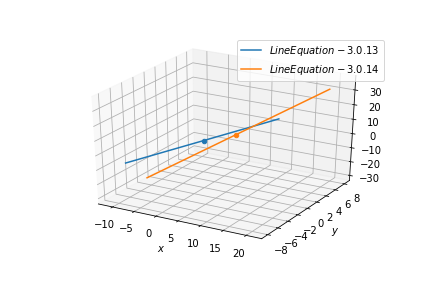
\includegraphics[width=\columnwidth]{./solutions/line_plane/74/codes/figs/Line_interest_2.png}
	\caption{Graph for equations \ref{eq:solutions/line_plane/74/codes14}}
	\label{fig:solutions/line_plane/74/codesline_equation_2}
\end{figure}
\end{enumerate}

    

\item If  $\begin{vmatrix}
x&2 \\ 18&x
\end{vmatrix}$ =$\begin{vmatrix}
6&2 \\ 18&6
\end{vmatrix}$, then x is equal to 
\begin{enumerate}
\item 6
\item $\pm 6$
\item $-6$
\item 0
\end{enumerate}
\item $\begin{vmatrix}
x&a&x+a\\y&b&y+b\\z&c&z+c\end{vmatrix}=0$
\\
\solution 
From theory, we understand that using dot product we can find the angle between the lines 
\begin{enumerate}
	\item 
	\begin{align}\label{eq:solutions/line_plane/74/codes:5}
		\frac{x-2}{2} = \frac{y-1}{5} &= \frac{z+3}{-3}, 
	\end{align}
	\begin{align}\label{eq:solutions/line_plane/74/codes:6}
		\frac{x+2}{-1} = \frac{y-4}{8} &= \frac{z-5}{4} 
	\end{align}


The above symmetric equations \ref{eq:solutions/line_plane/74/codes:5}, \ref{eq:solutions/line_plane/74/codes:6} can be represented in the vector form as 
\begin{align}\label{eq:solutions/line_plane/74/codes7}
	\quad \vec{r_1} &= \myvec{2\\1\\-3} + \lambda_1\myvec{2\\5\\-3}
	\\
	\quad \vec{r_2} &= \myvec{-2\\4\\5} + \lambda_2\myvec{-1\\8\\4}
\end{align}

As we have to find the angle between the vectors, we will only be taking the direction vectors into consideration. The direction vectors are $\vec{u}$ = $\myvec{2\\5\\-3}$ and $\vec{v}$ = $\myvec{-1\\8\\4}$. We can find the corresponding magnitude values

\begin{align}\label{eq:solutions/line_plane/74/codes9}
	\norm{\vec{u}} =\sqrt{2^{2}+5^{2}+(-3)^{2}} =\sqrt{38}
\end{align}
\begin{align}\label{eq:solutions/line_plane/74/codes10}
	\norm{\vec{v}} =\sqrt{(-1)^{2}+8^{2}+4^{2}} =\sqrt{81}
\end{align}

Using \ref{eq:solutions/line_plane/74/codes4}, \ref{eq:solutions/line_plane/74/codes9}, \ref{eq:solutions/line_plane/74/codes10} we get
\begin{align}
	\theta = \cos ^{-1}\frac{\myvec{2\\5\\-3}^{T}\myvec{-1\\8\\4}}{(\sqrt{38})(\sqrt{81})} 
	\\
	\theta = \cos ^{-1}\frac{26}{55.4797}
	\\
	\theta = \cos ^{-1} (0.4686)
	\\
	\theta = 62.053\degree
\end{align}

Therefore, the angle between the two lines is $62.053\degree$.See Fig. \ref{fig:solutions/line_plane/74/codesline_equation_1}

\begin{figure}
	\centering
	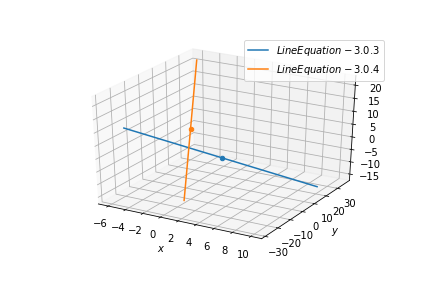
\includegraphics[width=\columnwidth]{./solutions/line_plane/74/codes/figs/Line_interest_1.png}
	\caption{Graph for equations \ref{eq:solutions/line_plane/74/codes7}}
	\label{fig:solutions/line_plane/74/codesline_equation_1}
\end{figure}


	\item 
	\begin{align}\label{eq:solutions/line_plane/74/codes12}
		\frac{x}{2} = \frac{y}{2} &= \frac{z}{1}, 
	\end{align}
	\begin{align}\label{eq:solutions/line_plane/74/codes13}
		\frac{x-5}{4} = \frac{y-2}{1} &= \frac{z-3}{8} 
	\end{align}



The above symmetric equations \ref{eq:solutions/line_plane/74/codes12}, \ref{eq:solutions/line_plane/74/codes13} can be represented in the vector form as 
\begin{align}\label{eq:solutions/line_plane/74/codes14}
	\quad \vec{r_1} &= \myvec{0\\0\\0} + \lambda_1\myvec{2\\2\\1}
	\\
	\quad \vec{r_2} &= \myvec{5\\2\\3} + \lambda_2\myvec{4\\1\\8}
\end{align}

As we have to find the angle between the vectors, we will only be taking the direction vectors into consideration. The direction vectors are $\vec{u}$ = $\myvec{2\\2\\1}$ and $\vec{v}$ = $\myvec{4\\1\\8}$. We can find the corresponding magnitude values

\begin{align}\label{eq:solutions/line_plane/74/codes16}
	\norm{\vec{u}} =\sqrt{2^{2}+2^{2}+1^{2}} =\sqrt{9}
\end{align}
\begin{align}\label{eq:solutions/line_plane/74/codes17}
	\norm{\vec{v}} =\sqrt{4^{2}+1^{2}+8^{2}} =\sqrt{81}
\end{align}

Using \ref{eq:solutions/line_plane/74/codes4}, \ref{eq:solutions/line_plane/74/codes16}, \ref{eq:solutions/line_plane/74/codes17} we get
\begin{align}
	\theta = \cos ^{-1}\frac{\myvec{2\\2\\1}^{T}\myvec{4\\1\\8}}{(\sqrt{9})(\sqrt{81})} 
	\\
	\theta = \cos ^{-1}\frac{18}{27.00}
	\\
	\theta = \cos ^{-1} (0.667)
	\\
	\theta = 48.189\degree
\end{align}

Therefore, the angle between the two lines is $48.189\degree$. See Fig. \ref{fig:solutions/line_plane/74/codesline_equation_2}


\begin{figure}
	\centering
	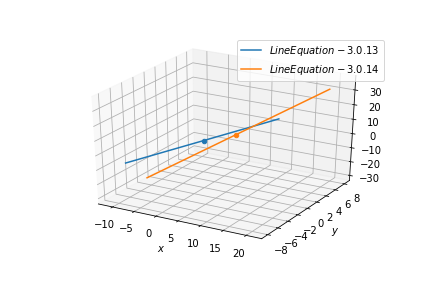
\includegraphics[width=\columnwidth]{./solutions/line_plane/74/codes/figs/Line_interest_2.png}
	\caption{Graph for equations \ref{eq:solutions/line_plane/74/codes14}}
	\label{fig:solutions/line_plane/74/codesline_equation_2}
\end{figure}
\end{enumerate}

    

\item $\begin{vmatrix}
a-b&b-c&c-a\\b-c&c-a&a-b\\c-a&a-b&b-c\end{vmatrix}=0$
\\
\solution 
From theory, we understand that using dot product we can find the angle between the lines 
\begin{enumerate}
	\item 
	\begin{align}\label{eq:solutions/line_plane/74/codes:5}
		\frac{x-2}{2} = \frac{y-1}{5} &= \frac{z+3}{-3}, 
	\end{align}
	\begin{align}\label{eq:solutions/line_plane/74/codes:6}
		\frac{x+2}{-1} = \frac{y-4}{8} &= \frac{z-5}{4} 
	\end{align}


The above symmetric equations \ref{eq:solutions/line_plane/74/codes:5}, \ref{eq:solutions/line_plane/74/codes:6} can be represented in the vector form as 
\begin{align}\label{eq:solutions/line_plane/74/codes7}
	\quad \vec{r_1} &= \myvec{2\\1\\-3} + \lambda_1\myvec{2\\5\\-3}
	\\
	\quad \vec{r_2} &= \myvec{-2\\4\\5} + \lambda_2\myvec{-1\\8\\4}
\end{align}

As we have to find the angle between the vectors, we will only be taking the direction vectors into consideration. The direction vectors are $\vec{u}$ = $\myvec{2\\5\\-3}$ and $\vec{v}$ = $\myvec{-1\\8\\4}$. We can find the corresponding magnitude values

\begin{align}\label{eq:solutions/line_plane/74/codes9}
	\norm{\vec{u}} =\sqrt{2^{2}+5^{2}+(-3)^{2}} =\sqrt{38}
\end{align}
\begin{align}\label{eq:solutions/line_plane/74/codes10}
	\norm{\vec{v}} =\sqrt{(-1)^{2}+8^{2}+4^{2}} =\sqrt{81}
\end{align}

Using \ref{eq:solutions/line_plane/74/codes4}, \ref{eq:solutions/line_plane/74/codes9}, \ref{eq:solutions/line_plane/74/codes10} we get
\begin{align}
	\theta = \cos ^{-1}\frac{\myvec{2\\5\\-3}^{T}\myvec{-1\\8\\4}}{(\sqrt{38})(\sqrt{81})} 
	\\
	\theta = \cos ^{-1}\frac{26}{55.4797}
	\\
	\theta = \cos ^{-1} (0.4686)
	\\
	\theta = 62.053\degree
\end{align}

Therefore, the angle between the two lines is $62.053\degree$.See Fig. \ref{fig:solutions/line_plane/74/codesline_equation_1}

\begin{figure}
	\centering
	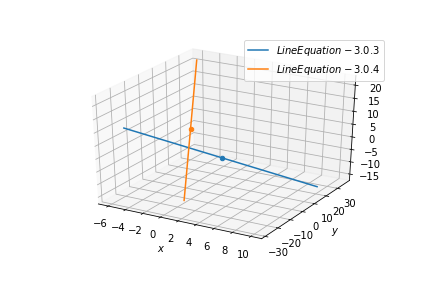
\includegraphics[width=\columnwidth]{./solutions/line_plane/74/codes/figs/Line_interest_1.png}
	\caption{Graph for equations \ref{eq:solutions/line_plane/74/codes7}}
	\label{fig:solutions/line_plane/74/codesline_equation_1}
\end{figure}


	\item 
	\begin{align}\label{eq:solutions/line_plane/74/codes12}
		\frac{x}{2} = \frac{y}{2} &= \frac{z}{1}, 
	\end{align}
	\begin{align}\label{eq:solutions/line_plane/74/codes13}
		\frac{x-5}{4} = \frac{y-2}{1} &= \frac{z-3}{8} 
	\end{align}



The above symmetric equations \ref{eq:solutions/line_plane/74/codes12}, \ref{eq:solutions/line_plane/74/codes13} can be represented in the vector form as 
\begin{align}\label{eq:solutions/line_plane/74/codes14}
	\quad \vec{r_1} &= \myvec{0\\0\\0} + \lambda_1\myvec{2\\2\\1}
	\\
	\quad \vec{r_2} &= \myvec{5\\2\\3} + \lambda_2\myvec{4\\1\\8}
\end{align}

As we have to find the angle between the vectors, we will only be taking the direction vectors into consideration. The direction vectors are $\vec{u}$ = $\myvec{2\\2\\1}$ and $\vec{v}$ = $\myvec{4\\1\\8}$. We can find the corresponding magnitude values

\begin{align}\label{eq:solutions/line_plane/74/codes16}
	\norm{\vec{u}} =\sqrt{2^{2}+2^{2}+1^{2}} =\sqrt{9}
\end{align}
\begin{align}\label{eq:solutions/line_plane/74/codes17}
	\norm{\vec{v}} =\sqrt{4^{2}+1^{2}+8^{2}} =\sqrt{81}
\end{align}

Using \ref{eq:solutions/line_plane/74/codes4}, \ref{eq:solutions/line_plane/74/codes16}, \ref{eq:solutions/line_plane/74/codes17} we get
\begin{align}
	\theta = \cos ^{-1}\frac{\myvec{2\\2\\1}^{T}\myvec{4\\1\\8}}{(\sqrt{9})(\sqrt{81})} 
	\\
	\theta = \cos ^{-1}\frac{18}{27.00}
	\\
	\theta = \cos ^{-1} (0.667)
	\\
	\theta = 48.189\degree
\end{align}

Therefore, the angle between the two lines is $48.189\degree$. See Fig. \ref{fig:solutions/line_plane/74/codesline_equation_2}


\begin{figure}
	\centering
	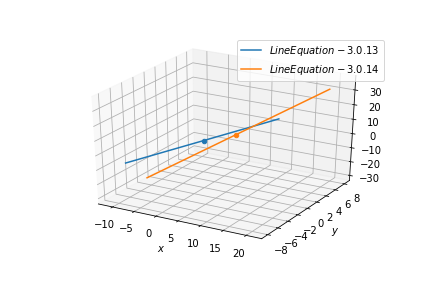
\includegraphics[width=\columnwidth]{./solutions/line_plane/74/codes/figs/Line_interest_2.png}
	\caption{Graph for equations \ref{eq:solutions/line_plane/74/codes14}}
	\label{fig:solutions/line_plane/74/codesline_equation_2}
\end{figure}
\end{enumerate}

    

\item $\begin{vmatrix}2&7&65\\3&8&75\\5&9&86\end{vmatrix}=0$
\\
\solution 
From theory, we understand that using dot product we can find the angle between the lines 
\begin{enumerate}
	\item 
	\begin{align}\label{eq:solutions/line_plane/74/codes:5}
		\frac{x-2}{2} = \frac{y-1}{5} &= \frac{z+3}{-3}, 
	\end{align}
	\begin{align}\label{eq:solutions/line_plane/74/codes:6}
		\frac{x+2}{-1} = \frac{y-4}{8} &= \frac{z-5}{4} 
	\end{align}


The above symmetric equations \ref{eq:solutions/line_plane/74/codes:5}, \ref{eq:solutions/line_plane/74/codes:6} can be represented in the vector form as 
\begin{align}\label{eq:solutions/line_plane/74/codes7}
	\quad \vec{r_1} &= \myvec{2\\1\\-3} + \lambda_1\myvec{2\\5\\-3}
	\\
	\quad \vec{r_2} &= \myvec{-2\\4\\5} + \lambda_2\myvec{-1\\8\\4}
\end{align}

As we have to find the angle between the vectors, we will only be taking the direction vectors into consideration. The direction vectors are $\vec{u}$ = $\myvec{2\\5\\-3}$ and $\vec{v}$ = $\myvec{-1\\8\\4}$. We can find the corresponding magnitude values

\begin{align}\label{eq:solutions/line_plane/74/codes9}
	\norm{\vec{u}} =\sqrt{2^{2}+5^{2}+(-3)^{2}} =\sqrt{38}
\end{align}
\begin{align}\label{eq:solutions/line_plane/74/codes10}
	\norm{\vec{v}} =\sqrt{(-1)^{2}+8^{2}+4^{2}} =\sqrt{81}
\end{align}

Using \ref{eq:solutions/line_plane/74/codes4}, \ref{eq:solutions/line_plane/74/codes9}, \ref{eq:solutions/line_plane/74/codes10} we get
\begin{align}
	\theta = \cos ^{-1}\frac{\myvec{2\\5\\-3}^{T}\myvec{-1\\8\\4}}{(\sqrt{38})(\sqrt{81})} 
	\\
	\theta = \cos ^{-1}\frac{26}{55.4797}
	\\
	\theta = \cos ^{-1} (0.4686)
	\\
	\theta = 62.053\degree
\end{align}

Therefore, the angle between the two lines is $62.053\degree$.See Fig. \ref{fig:solutions/line_plane/74/codesline_equation_1}

\begin{figure}
	\centering
	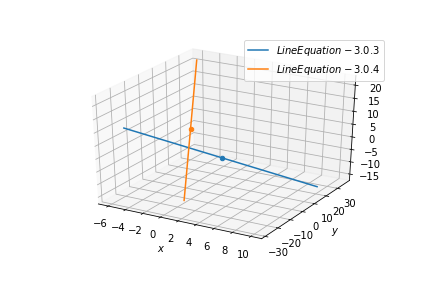
\includegraphics[width=\columnwidth]{./solutions/line_plane/74/codes/figs/Line_interest_1.png}
	\caption{Graph for equations \ref{eq:solutions/line_plane/74/codes7}}
	\label{fig:solutions/line_plane/74/codesline_equation_1}
\end{figure}


	\item 
	\begin{align}\label{eq:solutions/line_plane/74/codes12}
		\frac{x}{2} = \frac{y}{2} &= \frac{z}{1}, 
	\end{align}
	\begin{align}\label{eq:solutions/line_plane/74/codes13}
		\frac{x-5}{4} = \frac{y-2}{1} &= \frac{z-3}{8} 
	\end{align}



The above symmetric equations \ref{eq:solutions/line_plane/74/codes12}, \ref{eq:solutions/line_plane/74/codes13} can be represented in the vector form as 
\begin{align}\label{eq:solutions/line_plane/74/codes14}
	\quad \vec{r_1} &= \myvec{0\\0\\0} + \lambda_1\myvec{2\\2\\1}
	\\
	\quad \vec{r_2} &= \myvec{5\\2\\3} + \lambda_2\myvec{4\\1\\8}
\end{align}

As we have to find the angle between the vectors, we will only be taking the direction vectors into consideration. The direction vectors are $\vec{u}$ = $\myvec{2\\2\\1}$ and $\vec{v}$ = $\myvec{4\\1\\8}$. We can find the corresponding magnitude values

\begin{align}\label{eq:solutions/line_plane/74/codes16}
	\norm{\vec{u}} =\sqrt{2^{2}+2^{2}+1^{2}} =\sqrt{9}
\end{align}
\begin{align}\label{eq:solutions/line_plane/74/codes17}
	\norm{\vec{v}} =\sqrt{4^{2}+1^{2}+8^{2}} =\sqrt{81}
\end{align}

Using \ref{eq:solutions/line_plane/74/codes4}, \ref{eq:solutions/line_plane/74/codes16}, \ref{eq:solutions/line_plane/74/codes17} we get
\begin{align}
	\theta = \cos ^{-1}\frac{\myvec{2\\2\\1}^{T}\myvec{4\\1\\8}}{(\sqrt{9})(\sqrt{81})} 
	\\
	\theta = \cos ^{-1}\frac{18}{27.00}
	\\
	\theta = \cos ^{-1} (0.667)
	\\
	\theta = 48.189\degree
\end{align}

Therefore, the angle between the two lines is $48.189\degree$. See Fig. \ref{fig:solutions/line_plane/74/codesline_equation_2}


\begin{figure}
	\centering
	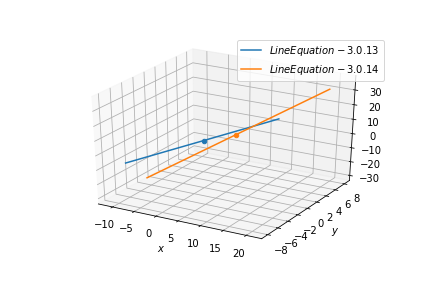
\includegraphics[width=\columnwidth]{./solutions/line_plane/74/codes/figs/Line_interest_2.png}
	\caption{Graph for equations \ref{eq:solutions/line_plane/74/codes14}}
	\label{fig:solutions/line_plane/74/codesline_equation_2}
\end{figure}
\end{enumerate}

    

\item $\begin{vmatrix}1&bc&a(b+c)\\1&ca&b(c+a)\\1&ab&c(a+b)\end{vmatrix}=0$
\\
\solution 
From theory, we understand that using dot product we can find the angle between the lines 
\begin{enumerate}
	\item 
	\begin{align}\label{eq:solutions/line_plane/74/codes:5}
		\frac{x-2}{2} = \frac{y-1}{5} &= \frac{z+3}{-3}, 
	\end{align}
	\begin{align}\label{eq:solutions/line_plane/74/codes:6}
		\frac{x+2}{-1} = \frac{y-4}{8} &= \frac{z-5}{4} 
	\end{align}


The above symmetric equations \ref{eq:solutions/line_plane/74/codes:5}, \ref{eq:solutions/line_plane/74/codes:6} can be represented in the vector form as 
\begin{align}\label{eq:solutions/line_plane/74/codes7}
	\quad \vec{r_1} &= \myvec{2\\1\\-3} + \lambda_1\myvec{2\\5\\-3}
	\\
	\quad \vec{r_2} &= \myvec{-2\\4\\5} + \lambda_2\myvec{-1\\8\\4}
\end{align}

As we have to find the angle between the vectors, we will only be taking the direction vectors into consideration. The direction vectors are $\vec{u}$ = $\myvec{2\\5\\-3}$ and $\vec{v}$ = $\myvec{-1\\8\\4}$. We can find the corresponding magnitude values

\begin{align}\label{eq:solutions/line_plane/74/codes9}
	\norm{\vec{u}} =\sqrt{2^{2}+5^{2}+(-3)^{2}} =\sqrt{38}
\end{align}
\begin{align}\label{eq:solutions/line_plane/74/codes10}
	\norm{\vec{v}} =\sqrt{(-1)^{2}+8^{2}+4^{2}} =\sqrt{81}
\end{align}

Using \ref{eq:solutions/line_plane/74/codes4}, \ref{eq:solutions/line_plane/74/codes9}, \ref{eq:solutions/line_plane/74/codes10} we get
\begin{align}
	\theta = \cos ^{-1}\frac{\myvec{2\\5\\-3}^{T}\myvec{-1\\8\\4}}{(\sqrt{38})(\sqrt{81})} 
	\\
	\theta = \cos ^{-1}\frac{26}{55.4797}
	\\
	\theta = \cos ^{-1} (0.4686)
	\\
	\theta = 62.053\degree
\end{align}

Therefore, the angle between the two lines is $62.053\degree$.See Fig. \ref{fig:solutions/line_plane/74/codesline_equation_1}

\begin{figure}
	\centering
	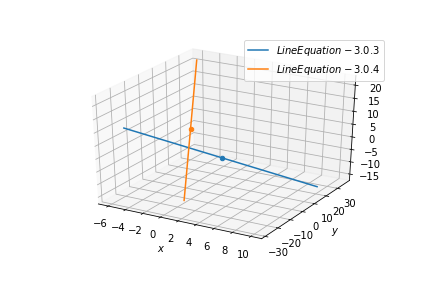
\includegraphics[width=\columnwidth]{./solutions/line_plane/74/codes/figs/Line_interest_1.png}
	\caption{Graph for equations \ref{eq:solutions/line_plane/74/codes7}}
	\label{fig:solutions/line_plane/74/codesline_equation_1}
\end{figure}


	\item 
	\begin{align}\label{eq:solutions/line_plane/74/codes12}
		\frac{x}{2} = \frac{y}{2} &= \frac{z}{1}, 
	\end{align}
	\begin{align}\label{eq:solutions/line_plane/74/codes13}
		\frac{x-5}{4} = \frac{y-2}{1} &= \frac{z-3}{8} 
	\end{align}



The above symmetric equations \ref{eq:solutions/line_plane/74/codes12}, \ref{eq:solutions/line_plane/74/codes13} can be represented in the vector form as 
\begin{align}\label{eq:solutions/line_plane/74/codes14}
	\quad \vec{r_1} &= \myvec{0\\0\\0} + \lambda_1\myvec{2\\2\\1}
	\\
	\quad \vec{r_2} &= \myvec{5\\2\\3} + \lambda_2\myvec{4\\1\\8}
\end{align}

As we have to find the angle between the vectors, we will only be taking the direction vectors into consideration. The direction vectors are $\vec{u}$ = $\myvec{2\\2\\1}$ and $\vec{v}$ = $\myvec{4\\1\\8}$. We can find the corresponding magnitude values

\begin{align}\label{eq:solutions/line_plane/74/codes16}
	\norm{\vec{u}} =\sqrt{2^{2}+2^{2}+1^{2}} =\sqrt{9}
\end{align}
\begin{align}\label{eq:solutions/line_plane/74/codes17}
	\norm{\vec{v}} =\sqrt{4^{2}+1^{2}+8^{2}} =\sqrt{81}
\end{align}

Using \ref{eq:solutions/line_plane/74/codes4}, \ref{eq:solutions/line_plane/74/codes16}, \ref{eq:solutions/line_plane/74/codes17} we get
\begin{align}
	\theta = \cos ^{-1}\frac{\myvec{2\\2\\1}^{T}\myvec{4\\1\\8}}{(\sqrt{9})(\sqrt{81})} 
	\\
	\theta = \cos ^{-1}\frac{18}{27.00}
	\\
	\theta = \cos ^{-1} (0.667)
	\\
	\theta = 48.189\degree
\end{align}

Therefore, the angle between the two lines is $48.189\degree$. See Fig. \ref{fig:solutions/line_plane/74/codesline_equation_2}


\begin{figure}
	\centering
	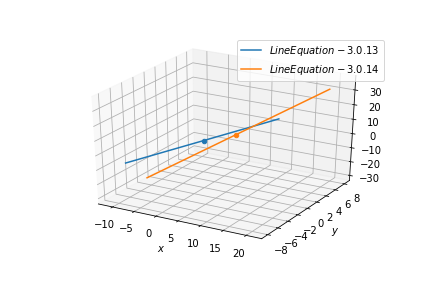
\includegraphics[width=\columnwidth]{./solutions/line_plane/74/codes/figs/Line_interest_2.png}
	\caption{Graph for equations \ref{eq:solutions/line_plane/74/codes14}}
	\label{fig:solutions/line_plane/74/codesline_equation_2}
\end{figure}
\end{enumerate}

    

\item $\begin{vmatrix}b+c& q+r& y+z\\c+a& r+p& z+x\\a+b& p+q& x+y\end{vmatrix}$=2$\begin{vmatrix} a&p&x\\b&q&y\\c&r&z\end{vmatrix}$ 
\\
\solution 
From theory, we understand that using dot product we can find the angle between the lines 
\begin{enumerate}
	\item 
	\begin{align}\label{eq:solutions/line_plane/74/codes:5}
		\frac{x-2}{2} = \frac{y-1}{5} &= \frac{z+3}{-3}, 
	\end{align}
	\begin{align}\label{eq:solutions/line_plane/74/codes:6}
		\frac{x+2}{-1} = \frac{y-4}{8} &= \frac{z-5}{4} 
	\end{align}


The above symmetric equations \ref{eq:solutions/line_plane/74/codes:5}, \ref{eq:solutions/line_plane/74/codes:6} can be represented in the vector form as 
\begin{align}\label{eq:solutions/line_plane/74/codes7}
	\quad \vec{r_1} &= \myvec{2\\1\\-3} + \lambda_1\myvec{2\\5\\-3}
	\\
	\quad \vec{r_2} &= \myvec{-2\\4\\5} + \lambda_2\myvec{-1\\8\\4}
\end{align}

As we have to find the angle between the vectors, we will only be taking the direction vectors into consideration. The direction vectors are $\vec{u}$ = $\myvec{2\\5\\-3}$ and $\vec{v}$ = $\myvec{-1\\8\\4}$. We can find the corresponding magnitude values

\begin{align}\label{eq:solutions/line_plane/74/codes9}
	\norm{\vec{u}} =\sqrt{2^{2}+5^{2}+(-3)^{2}} =\sqrt{38}
\end{align}
\begin{align}\label{eq:solutions/line_plane/74/codes10}
	\norm{\vec{v}} =\sqrt{(-1)^{2}+8^{2}+4^{2}} =\sqrt{81}
\end{align}

Using \ref{eq:solutions/line_plane/74/codes4}, \ref{eq:solutions/line_plane/74/codes9}, \ref{eq:solutions/line_plane/74/codes10} we get
\begin{align}
	\theta = \cos ^{-1}\frac{\myvec{2\\5\\-3}^{T}\myvec{-1\\8\\4}}{(\sqrt{38})(\sqrt{81})} 
	\\
	\theta = \cos ^{-1}\frac{26}{55.4797}
	\\
	\theta = \cos ^{-1} (0.4686)
	\\
	\theta = 62.053\degree
\end{align}

Therefore, the angle between the two lines is $62.053\degree$.See Fig. \ref{fig:solutions/line_plane/74/codesline_equation_1}

\begin{figure}
	\centering
	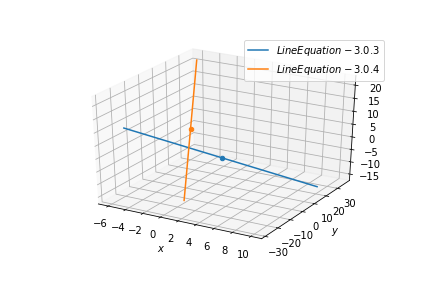
\includegraphics[width=\columnwidth]{./solutions/line_plane/74/codes/figs/Line_interest_1.png}
	\caption{Graph for equations \ref{eq:solutions/line_plane/74/codes7}}
	\label{fig:solutions/line_plane/74/codesline_equation_1}
\end{figure}


	\item 
	\begin{align}\label{eq:solutions/line_plane/74/codes12}
		\frac{x}{2} = \frac{y}{2} &= \frac{z}{1}, 
	\end{align}
	\begin{align}\label{eq:solutions/line_plane/74/codes13}
		\frac{x-5}{4} = \frac{y-2}{1} &= \frac{z-3}{8} 
	\end{align}



The above symmetric equations \ref{eq:solutions/line_plane/74/codes12}, \ref{eq:solutions/line_plane/74/codes13} can be represented in the vector form as 
\begin{align}\label{eq:solutions/line_plane/74/codes14}
	\quad \vec{r_1} &= \myvec{0\\0\\0} + \lambda_1\myvec{2\\2\\1}
	\\
	\quad \vec{r_2} &= \myvec{5\\2\\3} + \lambda_2\myvec{4\\1\\8}
\end{align}

As we have to find the angle between the vectors, we will only be taking the direction vectors into consideration. The direction vectors are $\vec{u}$ = $\myvec{2\\2\\1}$ and $\vec{v}$ = $\myvec{4\\1\\8}$. We can find the corresponding magnitude values

\begin{align}\label{eq:solutions/line_plane/74/codes16}
	\norm{\vec{u}} =\sqrt{2^{2}+2^{2}+1^{2}} =\sqrt{9}
\end{align}
\begin{align}\label{eq:solutions/line_plane/74/codes17}
	\norm{\vec{v}} =\sqrt{4^{2}+1^{2}+8^{2}} =\sqrt{81}
\end{align}

Using \ref{eq:solutions/line_plane/74/codes4}, \ref{eq:solutions/line_plane/74/codes16}, \ref{eq:solutions/line_plane/74/codes17} we get
\begin{align}
	\theta = \cos ^{-1}\frac{\myvec{2\\2\\1}^{T}\myvec{4\\1\\8}}{(\sqrt{9})(\sqrt{81})} 
	\\
	\theta = \cos ^{-1}\frac{18}{27.00}
	\\
	\theta = \cos ^{-1} (0.667)
	\\
	\theta = 48.189\degree
\end{align}

Therefore, the angle between the two lines is $48.189\degree$. See Fig. \ref{fig:solutions/line_plane/74/codesline_equation_2}


\begin{figure}
	\centering
	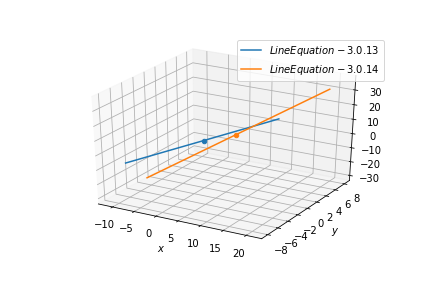
\includegraphics[width=\columnwidth]{./solutions/line_plane/74/codes/figs/Line_interest_2.png}
	\caption{Graph for equations \ref{eq:solutions/line_plane/74/codes14}}
	\label{fig:solutions/line_plane/74/codesline_equation_2}
\end{figure}
\end{enumerate}

    

\item $\begin{vmatrix}-a^2&ab&ab\\ ba&-b^2&bc\\ ca&cb&-c^2\end{vmatrix}$=$4a^2b^2c^2$\\
\\
\solution 
From theory, we understand that using dot product we can find the angle between the lines 
\begin{enumerate}
	\item 
	\begin{align}\label{eq:solutions/line_plane/74/codes:5}
		\frac{x-2}{2} = \frac{y-1}{5} &= \frac{z+3}{-3}, 
	\end{align}
	\begin{align}\label{eq:solutions/line_plane/74/codes:6}
		\frac{x+2}{-1} = \frac{y-4}{8} &= \frac{z-5}{4} 
	\end{align}


The above symmetric equations \ref{eq:solutions/line_plane/74/codes:5}, \ref{eq:solutions/line_plane/74/codes:6} can be represented in the vector form as 
\begin{align}\label{eq:solutions/line_plane/74/codes7}
	\quad \vec{r_1} &= \myvec{2\\1\\-3} + \lambda_1\myvec{2\\5\\-3}
	\\
	\quad \vec{r_2} &= \myvec{-2\\4\\5} + \lambda_2\myvec{-1\\8\\4}
\end{align}

As we have to find the angle between the vectors, we will only be taking the direction vectors into consideration. The direction vectors are $\vec{u}$ = $\myvec{2\\5\\-3}$ and $\vec{v}$ = $\myvec{-1\\8\\4}$. We can find the corresponding magnitude values

\begin{align}\label{eq:solutions/line_plane/74/codes9}
	\norm{\vec{u}} =\sqrt{2^{2}+5^{2}+(-3)^{2}} =\sqrt{38}
\end{align}
\begin{align}\label{eq:solutions/line_plane/74/codes10}
	\norm{\vec{v}} =\sqrt{(-1)^{2}+8^{2}+4^{2}} =\sqrt{81}
\end{align}

Using \ref{eq:solutions/line_plane/74/codes4}, \ref{eq:solutions/line_plane/74/codes9}, \ref{eq:solutions/line_plane/74/codes10} we get
\begin{align}
	\theta = \cos ^{-1}\frac{\myvec{2\\5\\-3}^{T}\myvec{-1\\8\\4}}{(\sqrt{38})(\sqrt{81})} 
	\\
	\theta = \cos ^{-1}\frac{26}{55.4797}
	\\
	\theta = \cos ^{-1} (0.4686)
	\\
	\theta = 62.053\degree
\end{align}

Therefore, the angle between the two lines is $62.053\degree$.See Fig. \ref{fig:solutions/line_plane/74/codesline_equation_1}

\begin{figure}
	\centering
	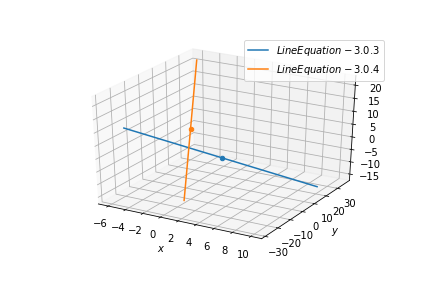
\includegraphics[width=\columnwidth]{./solutions/line_plane/74/codes/figs/Line_interest_1.png}
	\caption{Graph for equations \ref{eq:solutions/line_plane/74/codes7}}
	\label{fig:solutions/line_plane/74/codesline_equation_1}
\end{figure}


	\item 
	\begin{align}\label{eq:solutions/line_plane/74/codes12}
		\frac{x}{2} = \frac{y}{2} &= \frac{z}{1}, 
	\end{align}
	\begin{align}\label{eq:solutions/line_plane/74/codes13}
		\frac{x-5}{4} = \frac{y-2}{1} &= \frac{z-3}{8} 
	\end{align}



The above symmetric equations \ref{eq:solutions/line_plane/74/codes12}, \ref{eq:solutions/line_plane/74/codes13} can be represented in the vector form as 
\begin{align}\label{eq:solutions/line_plane/74/codes14}
	\quad \vec{r_1} &= \myvec{0\\0\\0} + \lambda_1\myvec{2\\2\\1}
	\\
	\quad \vec{r_2} &= \myvec{5\\2\\3} + \lambda_2\myvec{4\\1\\8}
\end{align}

As we have to find the angle between the vectors, we will only be taking the direction vectors into consideration. The direction vectors are $\vec{u}$ = $\myvec{2\\2\\1}$ and $\vec{v}$ = $\myvec{4\\1\\8}$. We can find the corresponding magnitude values

\begin{align}\label{eq:solutions/line_plane/74/codes16}
	\norm{\vec{u}} =\sqrt{2^{2}+2^{2}+1^{2}} =\sqrt{9}
\end{align}
\begin{align}\label{eq:solutions/line_plane/74/codes17}
	\norm{\vec{v}} =\sqrt{4^{2}+1^{2}+8^{2}} =\sqrt{81}
\end{align}

Using \ref{eq:solutions/line_plane/74/codes4}, \ref{eq:solutions/line_plane/74/codes16}, \ref{eq:solutions/line_plane/74/codes17} we get
\begin{align}
	\theta = \cos ^{-1}\frac{\myvec{2\\2\\1}^{T}\myvec{4\\1\\8}}{(\sqrt{9})(\sqrt{81})} 
	\\
	\theta = \cos ^{-1}\frac{18}{27.00}
	\\
	\theta = \cos ^{-1} (0.667)
	\\
	\theta = 48.189\degree
\end{align}

Therefore, the angle between the two lines is $48.189\degree$. See Fig. \ref{fig:solutions/line_plane/74/codesline_equation_2}


\begin{figure}
	\centering
	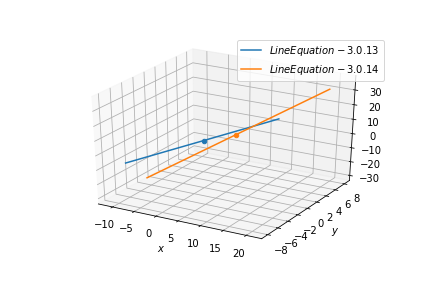
\includegraphics[width=\columnwidth]{./solutions/line_plane/74/codes/figs/Line_interest_2.png}
	\caption{Graph for equations \ref{eq:solutions/line_plane/74/codes14}}
	\label{fig:solutions/line_plane/74/codesline_equation_2}
\end{figure}
\end{enumerate}

    

By Using properties of determinants, in Exercises 16 to 22,Show that;
\item (i)$\begin{vmatrix}1&a&a^2\\1&b&b^2\\1&c&c^2\end{vmatrix}$=(a-b)(b-c)(c-a)\\
(ii) $\begin{vmatrix}1&1&1 \\ a&b&c \\ a^3&b^3&c^3\end{vmatrix}$=(a-b)(b-c)(c-a)(a+b+c)
\\
\solution 
From theory, we understand that using dot product we can find the angle between the lines 
\begin{enumerate}
	\item 
	\begin{align}\label{eq:solutions/line_plane/74/codes:5}
		\frac{x-2}{2} = \frac{y-1}{5} &= \frac{z+3}{-3}, 
	\end{align}
	\begin{align}\label{eq:solutions/line_plane/74/codes:6}
		\frac{x+2}{-1} = \frac{y-4}{8} &= \frac{z-5}{4} 
	\end{align}


The above symmetric equations \ref{eq:solutions/line_plane/74/codes:5}, \ref{eq:solutions/line_plane/74/codes:6} can be represented in the vector form as 
\begin{align}\label{eq:solutions/line_plane/74/codes7}
	\quad \vec{r_1} &= \myvec{2\\1\\-3} + \lambda_1\myvec{2\\5\\-3}
	\\
	\quad \vec{r_2} &= \myvec{-2\\4\\5} + \lambda_2\myvec{-1\\8\\4}
\end{align}

As we have to find the angle between the vectors, we will only be taking the direction vectors into consideration. The direction vectors are $\vec{u}$ = $\myvec{2\\5\\-3}$ and $\vec{v}$ = $\myvec{-1\\8\\4}$. We can find the corresponding magnitude values

\begin{align}\label{eq:solutions/line_plane/74/codes9}
	\norm{\vec{u}} =\sqrt{2^{2}+5^{2}+(-3)^{2}} =\sqrt{38}
\end{align}
\begin{align}\label{eq:solutions/line_plane/74/codes10}
	\norm{\vec{v}} =\sqrt{(-1)^{2}+8^{2}+4^{2}} =\sqrt{81}
\end{align}

Using \ref{eq:solutions/line_plane/74/codes4}, \ref{eq:solutions/line_plane/74/codes9}, \ref{eq:solutions/line_plane/74/codes10} we get
\begin{align}
	\theta = \cos ^{-1}\frac{\myvec{2\\5\\-3}^{T}\myvec{-1\\8\\4}}{(\sqrt{38})(\sqrt{81})} 
	\\
	\theta = \cos ^{-1}\frac{26}{55.4797}
	\\
	\theta = \cos ^{-1} (0.4686)
	\\
	\theta = 62.053\degree
\end{align}

Therefore, the angle between the two lines is $62.053\degree$.See Fig. \ref{fig:solutions/line_plane/74/codesline_equation_1}

\begin{figure}
	\centering
	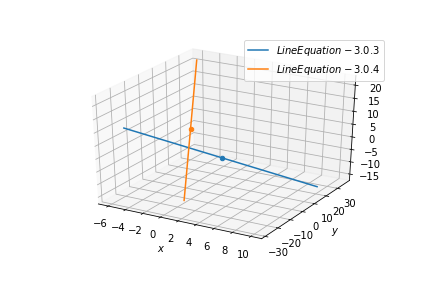
\includegraphics[width=\columnwidth]{./solutions/line_plane/74/codes/figs/Line_interest_1.png}
	\caption{Graph for equations \ref{eq:solutions/line_plane/74/codes7}}
	\label{fig:solutions/line_plane/74/codesline_equation_1}
\end{figure}


	\item 
	\begin{align}\label{eq:solutions/line_plane/74/codes12}
		\frac{x}{2} = \frac{y}{2} &= \frac{z}{1}, 
	\end{align}
	\begin{align}\label{eq:solutions/line_plane/74/codes13}
		\frac{x-5}{4} = \frac{y-2}{1} &= \frac{z-3}{8} 
	\end{align}



The above symmetric equations \ref{eq:solutions/line_plane/74/codes12}, \ref{eq:solutions/line_plane/74/codes13} can be represented in the vector form as 
\begin{align}\label{eq:solutions/line_plane/74/codes14}
	\quad \vec{r_1} &= \myvec{0\\0\\0} + \lambda_1\myvec{2\\2\\1}
	\\
	\quad \vec{r_2} &= \myvec{5\\2\\3} + \lambda_2\myvec{4\\1\\8}
\end{align}

As we have to find the angle between the vectors, we will only be taking the direction vectors into consideration. The direction vectors are $\vec{u}$ = $\myvec{2\\2\\1}$ and $\vec{v}$ = $\myvec{4\\1\\8}$. We can find the corresponding magnitude values

\begin{align}\label{eq:solutions/line_plane/74/codes16}
	\norm{\vec{u}} =\sqrt{2^{2}+2^{2}+1^{2}} =\sqrt{9}
\end{align}
\begin{align}\label{eq:solutions/line_plane/74/codes17}
	\norm{\vec{v}} =\sqrt{4^{2}+1^{2}+8^{2}} =\sqrt{81}
\end{align}

Using \ref{eq:solutions/line_plane/74/codes4}, \ref{eq:solutions/line_plane/74/codes16}, \ref{eq:solutions/line_plane/74/codes17} we get
\begin{align}
	\theta = \cos ^{-1}\frac{\myvec{2\\2\\1}^{T}\myvec{4\\1\\8}}{(\sqrt{9})(\sqrt{81})} 
	\\
	\theta = \cos ^{-1}\frac{18}{27.00}
	\\
	\theta = \cos ^{-1} (0.667)
	\\
	\theta = 48.189\degree
\end{align}

Therefore, the angle between the two lines is $48.189\degree$. See Fig. \ref{fig:solutions/line_plane/74/codesline_equation_2}


\begin{figure}
	\centering
	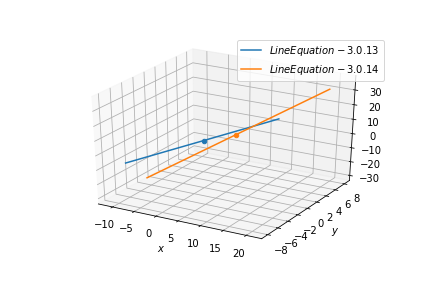
\includegraphics[width=\columnwidth]{./solutions/line_plane/74/codes/figs/Line_interest_2.png}
	\caption{Graph for equations \ref{eq:solutions/line_plane/74/codes14}}
	\label{fig:solutions/line_plane/74/codesline_equation_2}
\end{figure}
\end{enumerate}

    

\item $\begin{vmatrix}x&x^2&yz \\ y&y^2&zx \\ z&z^2&xy\end{vmatrix}$=(x-y)(y-z)(z-x)(xy+yz+zx)
\item (i) $\begin{vmatrix}x+4&2x&2x \\ 2x&x+4&2x \\ 2x&2x&x+4\end{vmatrix}$=$(5x+4)(4-x)^2$\\
\solution 
From theory, we understand that using dot product we can find the angle between the lines 
\begin{enumerate}
	\item 
	\begin{align}\label{eq:solutions/line_plane/74/codes:5}
		\frac{x-2}{2} = \frac{y-1}{5} &= \frac{z+3}{-3}, 
	\end{align}
	\begin{align}\label{eq:solutions/line_plane/74/codes:6}
		\frac{x+2}{-1} = \frac{y-4}{8} &= \frac{z-5}{4} 
	\end{align}


The above symmetric equations \ref{eq:solutions/line_plane/74/codes:5}, \ref{eq:solutions/line_plane/74/codes:6} can be represented in the vector form as 
\begin{align}\label{eq:solutions/line_plane/74/codes7}
	\quad \vec{r_1} &= \myvec{2\\1\\-3} + \lambda_1\myvec{2\\5\\-3}
	\\
	\quad \vec{r_2} &= \myvec{-2\\4\\5} + \lambda_2\myvec{-1\\8\\4}
\end{align}

As we have to find the angle between the vectors, we will only be taking the direction vectors into consideration. The direction vectors are $\vec{u}$ = $\myvec{2\\5\\-3}$ and $\vec{v}$ = $\myvec{-1\\8\\4}$. We can find the corresponding magnitude values

\begin{align}\label{eq:solutions/line_plane/74/codes9}
	\norm{\vec{u}} =\sqrt{2^{2}+5^{2}+(-3)^{2}} =\sqrt{38}
\end{align}
\begin{align}\label{eq:solutions/line_plane/74/codes10}
	\norm{\vec{v}} =\sqrt{(-1)^{2}+8^{2}+4^{2}} =\sqrt{81}
\end{align}

Using \ref{eq:solutions/line_plane/74/codes4}, \ref{eq:solutions/line_plane/74/codes9}, \ref{eq:solutions/line_plane/74/codes10} we get
\begin{align}
	\theta = \cos ^{-1}\frac{\myvec{2\\5\\-3}^{T}\myvec{-1\\8\\4}}{(\sqrt{38})(\sqrt{81})} 
	\\
	\theta = \cos ^{-1}\frac{26}{55.4797}
	\\
	\theta = \cos ^{-1} (0.4686)
	\\
	\theta = 62.053\degree
\end{align}

Therefore, the angle between the two lines is $62.053\degree$.See Fig. \ref{fig:solutions/line_plane/74/codesline_equation_1}

\begin{figure}
	\centering
	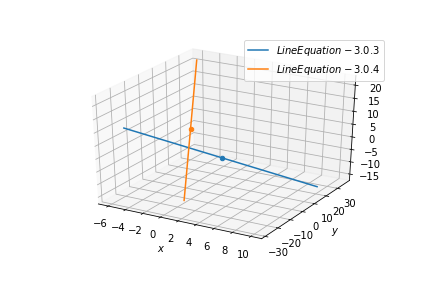
\includegraphics[width=\columnwidth]{./solutions/line_plane/74/codes/figs/Line_interest_1.png}
	\caption{Graph for equations \ref{eq:solutions/line_plane/74/codes7}}
	\label{fig:solutions/line_plane/74/codesline_equation_1}
\end{figure}


	\item 
	\begin{align}\label{eq:solutions/line_plane/74/codes12}
		\frac{x}{2} = \frac{y}{2} &= \frac{z}{1}, 
	\end{align}
	\begin{align}\label{eq:solutions/line_plane/74/codes13}
		\frac{x-5}{4} = \frac{y-2}{1} &= \frac{z-3}{8} 
	\end{align}



The above symmetric equations \ref{eq:solutions/line_plane/74/codes12}, \ref{eq:solutions/line_plane/74/codes13} can be represented in the vector form as 
\begin{align}\label{eq:solutions/line_plane/74/codes14}
	\quad \vec{r_1} &= \myvec{0\\0\\0} + \lambda_1\myvec{2\\2\\1}
	\\
	\quad \vec{r_2} &= \myvec{5\\2\\3} + \lambda_2\myvec{4\\1\\8}
\end{align}

As we have to find the angle between the vectors, we will only be taking the direction vectors into consideration. The direction vectors are $\vec{u}$ = $\myvec{2\\2\\1}$ and $\vec{v}$ = $\myvec{4\\1\\8}$. We can find the corresponding magnitude values

\begin{align}\label{eq:solutions/line_plane/74/codes16}
	\norm{\vec{u}} =\sqrt{2^{2}+2^{2}+1^{2}} =\sqrt{9}
\end{align}
\begin{align}\label{eq:solutions/line_plane/74/codes17}
	\norm{\vec{v}} =\sqrt{4^{2}+1^{2}+8^{2}} =\sqrt{81}
\end{align}

Using \ref{eq:solutions/line_plane/74/codes4}, \ref{eq:solutions/line_plane/74/codes16}, \ref{eq:solutions/line_plane/74/codes17} we get
\begin{align}
	\theta = \cos ^{-1}\frac{\myvec{2\\2\\1}^{T}\myvec{4\\1\\8}}{(\sqrt{9})(\sqrt{81})} 
	\\
	\theta = \cos ^{-1}\frac{18}{27.00}
	\\
	\theta = \cos ^{-1} (0.667)
	\\
	\theta = 48.189\degree
\end{align}

Therefore, the angle between the two lines is $48.189\degree$. See Fig. \ref{fig:solutions/line_plane/74/codesline_equation_2}


\begin{figure}
	\centering
	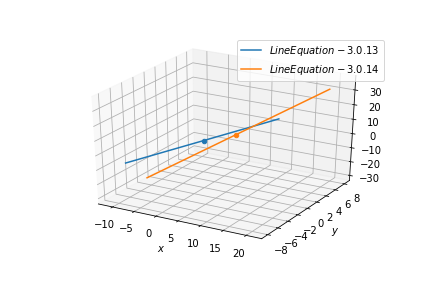
\includegraphics[width=\columnwidth]{./solutions/line_plane/74/codes/figs/Line_interest_2.png}
	\caption{Graph for equations \ref{eq:solutions/line_plane/74/codes14}}
	\label{fig:solutions/line_plane/74/codesline_equation_2}
\end{figure}
\end{enumerate}

    

(ii) $\begin{vmatrix}y+k&y&y \\ y&y+k&y \\ y&y&xy+k\end{vmatrix}$=$k^2(3y+k)$
\\
\solution 
From theory, we understand that using dot product we can find the angle between the lines 
\begin{enumerate}
	\item 
	\begin{align}\label{eq:solutions/line_plane/74/codes:5}
		\frac{x-2}{2} = \frac{y-1}{5} &= \frac{z+3}{-3}, 
	\end{align}
	\begin{align}\label{eq:solutions/line_plane/74/codes:6}
		\frac{x+2}{-1} = \frac{y-4}{8} &= \frac{z-5}{4} 
	\end{align}


The above symmetric equations \ref{eq:solutions/line_plane/74/codes:5}, \ref{eq:solutions/line_plane/74/codes:6} can be represented in the vector form as 
\begin{align}\label{eq:solutions/line_plane/74/codes7}
	\quad \vec{r_1} &= \myvec{2\\1\\-3} + \lambda_1\myvec{2\\5\\-3}
	\\
	\quad \vec{r_2} &= \myvec{-2\\4\\5} + \lambda_2\myvec{-1\\8\\4}
\end{align}

As we have to find the angle between the vectors, we will only be taking the direction vectors into consideration. The direction vectors are $\vec{u}$ = $\myvec{2\\5\\-3}$ and $\vec{v}$ = $\myvec{-1\\8\\4}$. We can find the corresponding magnitude values

\begin{align}\label{eq:solutions/line_plane/74/codes9}
	\norm{\vec{u}} =\sqrt{2^{2}+5^{2}+(-3)^{2}} =\sqrt{38}
\end{align}
\begin{align}\label{eq:solutions/line_plane/74/codes10}
	\norm{\vec{v}} =\sqrt{(-1)^{2}+8^{2}+4^{2}} =\sqrt{81}
\end{align}

Using \ref{eq:solutions/line_plane/74/codes4}, \ref{eq:solutions/line_plane/74/codes9}, \ref{eq:solutions/line_plane/74/codes10} we get
\begin{align}
	\theta = \cos ^{-1}\frac{\myvec{2\\5\\-3}^{T}\myvec{-1\\8\\4}}{(\sqrt{38})(\sqrt{81})} 
	\\
	\theta = \cos ^{-1}\frac{26}{55.4797}
	\\
	\theta = \cos ^{-1} (0.4686)
	\\
	\theta = 62.053\degree
\end{align}

Therefore, the angle between the two lines is $62.053\degree$.See Fig. \ref{fig:solutions/line_plane/74/codesline_equation_1}

\begin{figure}
	\centering
	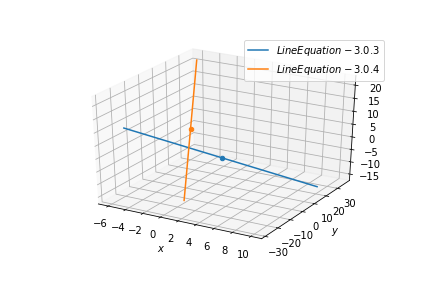
\includegraphics[width=\columnwidth]{./solutions/line_plane/74/codes/figs/Line_interest_1.png}
	\caption{Graph for equations \ref{eq:solutions/line_plane/74/codes7}}
	\label{fig:solutions/line_plane/74/codesline_equation_1}
\end{figure}


	\item 
	\begin{align}\label{eq:solutions/line_plane/74/codes12}
		\frac{x}{2} = \frac{y}{2} &= \frac{z}{1}, 
	\end{align}
	\begin{align}\label{eq:solutions/line_plane/74/codes13}
		\frac{x-5}{4} = \frac{y-2}{1} &= \frac{z-3}{8} 
	\end{align}



The above symmetric equations \ref{eq:solutions/line_plane/74/codes12}, \ref{eq:solutions/line_plane/74/codes13} can be represented in the vector form as 
\begin{align}\label{eq:solutions/line_plane/74/codes14}
	\quad \vec{r_1} &= \myvec{0\\0\\0} + \lambda_1\myvec{2\\2\\1}
	\\
	\quad \vec{r_2} &= \myvec{5\\2\\3} + \lambda_2\myvec{4\\1\\8}
\end{align}

As we have to find the angle between the vectors, we will only be taking the direction vectors into consideration. The direction vectors are $\vec{u}$ = $\myvec{2\\2\\1}$ and $\vec{v}$ = $\myvec{4\\1\\8}$. We can find the corresponding magnitude values

\begin{align}\label{eq:solutions/line_plane/74/codes16}
	\norm{\vec{u}} =\sqrt{2^{2}+2^{2}+1^{2}} =\sqrt{9}
\end{align}
\begin{align}\label{eq:solutions/line_plane/74/codes17}
	\norm{\vec{v}} =\sqrt{4^{2}+1^{2}+8^{2}} =\sqrt{81}
\end{align}

Using \ref{eq:solutions/line_plane/74/codes4}, \ref{eq:solutions/line_plane/74/codes16}, \ref{eq:solutions/line_plane/74/codes17} we get
\begin{align}
	\theta = \cos ^{-1}\frac{\myvec{2\\2\\1}^{T}\myvec{4\\1\\8}}{(\sqrt{9})(\sqrt{81})} 
	\\
	\theta = \cos ^{-1}\frac{18}{27.00}
	\\
	\theta = \cos ^{-1} (0.667)
	\\
	\theta = 48.189\degree
\end{align}

Therefore, the angle between the two lines is $48.189\degree$. See Fig. \ref{fig:solutions/line_plane/74/codesline_equation_2}


\begin{figure}
	\centering
	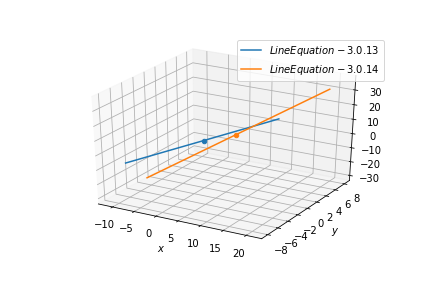
\includegraphics[width=\columnwidth]{./solutions/line_plane/74/codes/figs/Line_interest_2.png}
	\caption{Graph for equations \ref{eq:solutions/line_plane/74/codes14}}
	\label{fig:solutions/line_plane/74/codesline_equation_2}
\end{figure}
\end{enumerate}

    


\item $\begin{vmatrix}a^2+1&ab&ac \\ ab&b^2+1&bc \\ ca&cb&c^2+1\end{vmatrix}$=$1+a^2+b^2+c^2$\\
\\
\solution 
From theory, we understand that using dot product we can find the angle between the lines 
\begin{enumerate}
	\item 
	\begin{align}\label{eq:solutions/line_plane/74/codes:5}
		\frac{x-2}{2} = \frac{y-1}{5} &= \frac{z+3}{-3}, 
	\end{align}
	\begin{align}\label{eq:solutions/line_plane/74/codes:6}
		\frac{x+2}{-1} = \frac{y-4}{8} &= \frac{z-5}{4} 
	\end{align}


The above symmetric equations \ref{eq:solutions/line_plane/74/codes:5}, \ref{eq:solutions/line_plane/74/codes:6} can be represented in the vector form as 
\begin{align}\label{eq:solutions/line_plane/74/codes7}
	\quad \vec{r_1} &= \myvec{2\\1\\-3} + \lambda_1\myvec{2\\5\\-3}
	\\
	\quad \vec{r_2} &= \myvec{-2\\4\\5} + \lambda_2\myvec{-1\\8\\4}
\end{align}

As we have to find the angle between the vectors, we will only be taking the direction vectors into consideration. The direction vectors are $\vec{u}$ = $\myvec{2\\5\\-3}$ and $\vec{v}$ = $\myvec{-1\\8\\4}$. We can find the corresponding magnitude values

\begin{align}\label{eq:solutions/line_plane/74/codes9}
	\norm{\vec{u}} =\sqrt{2^{2}+5^{2}+(-3)^{2}} =\sqrt{38}
\end{align}
\begin{align}\label{eq:solutions/line_plane/74/codes10}
	\norm{\vec{v}} =\sqrt{(-1)^{2}+8^{2}+4^{2}} =\sqrt{81}
\end{align}

Using \ref{eq:solutions/line_plane/74/codes4}, \ref{eq:solutions/line_plane/74/codes9}, \ref{eq:solutions/line_plane/74/codes10} we get
\begin{align}
	\theta = \cos ^{-1}\frac{\myvec{2\\5\\-3}^{T}\myvec{-1\\8\\4}}{(\sqrt{38})(\sqrt{81})} 
	\\
	\theta = \cos ^{-1}\frac{26}{55.4797}
	\\
	\theta = \cos ^{-1} (0.4686)
	\\
	\theta = 62.053\degree
\end{align}

Therefore, the angle between the two lines is $62.053\degree$.See Fig. \ref{fig:solutions/line_plane/74/codesline_equation_1}

\begin{figure}
	\centering
	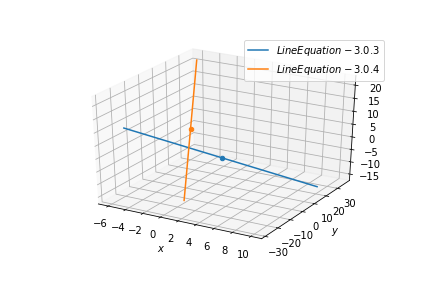
\includegraphics[width=\columnwidth]{./solutions/line_plane/74/codes/figs/Line_interest_1.png}
	\caption{Graph for equations \ref{eq:solutions/line_plane/74/codes7}}
	\label{fig:solutions/line_plane/74/codesline_equation_1}
\end{figure}


	\item 
	\begin{align}\label{eq:solutions/line_plane/74/codes12}
		\frac{x}{2} = \frac{y}{2} &= \frac{z}{1}, 
	\end{align}
	\begin{align}\label{eq:solutions/line_plane/74/codes13}
		\frac{x-5}{4} = \frac{y-2}{1} &= \frac{z-3}{8} 
	\end{align}



The above symmetric equations \ref{eq:solutions/line_plane/74/codes12}, \ref{eq:solutions/line_plane/74/codes13} can be represented in the vector form as 
\begin{align}\label{eq:solutions/line_plane/74/codes14}
	\quad \vec{r_1} &= \myvec{0\\0\\0} + \lambda_1\myvec{2\\2\\1}
	\\
	\quad \vec{r_2} &= \myvec{5\\2\\3} + \lambda_2\myvec{4\\1\\8}
\end{align}

As we have to find the angle between the vectors, we will only be taking the direction vectors into consideration. The direction vectors are $\vec{u}$ = $\myvec{2\\2\\1}$ and $\vec{v}$ = $\myvec{4\\1\\8}$. We can find the corresponding magnitude values

\begin{align}\label{eq:solutions/line_plane/74/codes16}
	\norm{\vec{u}} =\sqrt{2^{2}+2^{2}+1^{2}} =\sqrt{9}
\end{align}
\begin{align}\label{eq:solutions/line_plane/74/codes17}
	\norm{\vec{v}} =\sqrt{4^{2}+1^{2}+8^{2}} =\sqrt{81}
\end{align}

Using \ref{eq:solutions/line_plane/74/codes4}, \ref{eq:solutions/line_plane/74/codes16}, \ref{eq:solutions/line_plane/74/codes17} we get
\begin{align}
	\theta = \cos ^{-1}\frac{\myvec{2\\2\\1}^{T}\myvec{4\\1\\8}}{(\sqrt{9})(\sqrt{81})} 
	\\
	\theta = \cos ^{-1}\frac{18}{27.00}
	\\
	\theta = \cos ^{-1} (0.667)
	\\
	\theta = 48.189\degree
\end{align}

Therefore, the angle between the two lines is $48.189\degree$. See Fig. \ref{fig:solutions/line_plane/74/codesline_equation_2}


\begin{figure}
	\centering
	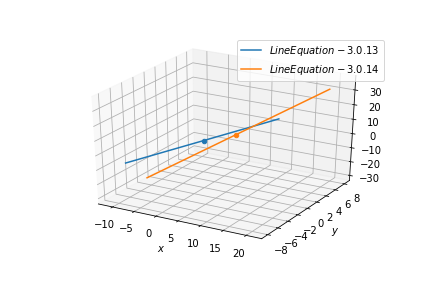
\includegraphics[width=\columnwidth]{./solutions/line_plane/74/codes/figs/Line_interest_2.png}
	\caption{Graph for equations \ref{eq:solutions/line_plane/74/codes14}}
	\label{fig:solutions/line_plane/74/codesline_equation_2}
\end{figure}
\end{enumerate}

    

Choose the correct answer in Exercises 23 and 24.
\item Let A be a square matrix of order 3X3, then 
$\abs{kA}$ is equal to
\begin{enumerate}
\item $k\abs{A}$
\item $k^2\abs{A}$
\item $k^3\abs{A}$
\item $3k\abs{A}$
\end{enumerate} 
\item Which of the following is correct
\begin{enumerate}
\item Determinant is a square matrix.
\item Determinant is a number associated to a matrix.
\item Determinant is a number associated to a square matrix.
\item None of these.
\end{enumerate}
\item Find area of the triangle with vertices at the point given in each of the following :\\
(i) \myvec{1&0}, \myvec{6&0}, \myvec{4&3}\\
(ii) \myvec{2&7}, \myvec{1&1}, \myvec{10&8}\\
(iii) \myvec{-2&-3}, \myvec{3&2}, \myvec{-1&-8}\\
\solution 
\begin{enumerate}
    \item 
    
\begin{table}[!ht]
\centering
\resizebox{\columnwidth}{!}{\begin{tabular}{|c|c|c|c|} 
\hline
kind of  cake & No.of cakes & Flour& Fat\\
\hline
1st & x & 200g  &  25g \\ 
\hline
2nd& y& 100g&  50g  \\ 
\hline
Total& x+y& 5 kg=5000g&1kg=1000g \\ 
\hline
\end{tabular}}
\caption{Ingredients used in making the cake is flour and fat }
\label{opt/13/tab:table1}
\end{table}
Let the  1st kind  be $x$ and the 2nd kind be $y$  such that 
\begin{align}
x \geq 0 \\
y \geq 0 
\end{align}
According to the question,
\begin{align}
2{x} + {y} \leq 50
\\
{x} + 2{y} \leq 40
\end{align}
$\therefore$ Our problem is
\begin{align}
\max_{\vec{x}} Z &= \myvec{1& 1}\vec{x}\\
s.t. \quad \myvec{2 & 1 \\ 1& 2}\vec{x} &\preceq \myvec{50\\40} 
\end{align}
Lagrangian function is given by
\begin{equation}
\begin{aligned}
&L(\vec{x},\boldsymbol{\lambda}) \\ &= \myvec{1 & 1}\vec{x}+\lcbrak{\sbrak{\myvec{2 & 1}\vec{x}-50}} \\ &+ \sbrak{\myvec{1 & 2}\vec{x}-40}\\ &+ \sbrak{\myvec{-1 & 0}\vec{x}} +\rcbrak{\sbrak{\myvec{0 & -1}\vec{x}}}\boldsymbol{\lambda}
\end{aligned}
\end{equation}
where,
\begin{align}
\boldsymbol{\lambda} &= \myvec{\lambda_1 \\ \lambda_2 \\ \lambda_3 \\ \lambda_4 \\ \lambda_5 \\ \lambda_6}
\end{align}
Now,
\begin{align}
\nabla L(\vec{x},\boldsymbol{\lambda}) &= \myvec{1+ \myvec{2 & 1 & -1 & 0 }\boldsymbol{\lambda}\\ 1+\myvec{1 & 2 & 0 & -1}\boldsymbol{\lambda} \\ \myvec{2 & 1}\vec{x}-50\\ \myvec{1& 2}\vec{x}-40 \\  \myvec{-1 & 0}\vec{x} \\ \myvec{0 & -1}\vec{x}}
\end{align}
$\therefore$ Lagrangian matrix is given by
\begin{align}
\myvec{0 & 0 & 2 & 1& -1 & 0 \\ 0 & 0 & 1 & 2  & 0 & -1 \\ 2 & 1 & 0 & 0 & 0 & 0 \\ 1 & 2 & 0 & 0 & 0 & 0  \\ -1 & 0 & 0 & 0 & 0 & 0  \\ 0 & -1 & 0 & 0 & 0 & 0 }\myvec{\vec{x} \\ \boldsymbol{\lambda} } &= \myvec{-1 \\ -1 \\ 50\\ 4 0\\ 0 \\0 }
\end{align}
Considering $\lambda_1,\lambda_2$ as only active multiplier,
\begin{align}
\myvec{0 & 0 & 2 & 1 \\ 0 & 0 & 1 & 2 \\ 2 & 1 & 0 & 0 \\ 1 & 2 & 0 & 0}\myvec{\vec{x}\\ \boldsymbol{\lambda}} &= \myvec{-1 \\ -1 \\ 5 0\\ 40}
\end{align}
resulting in,
\begin{align}
\myvec{\vec{x} \\ \boldsymbol{\lambda}} &= \myvec{0 & 0 & 2 & 1 \\ 0 & 0 & 1 & 2 \\ 2 & 1 & 0 & 0 \\ 1& 2 & 0 & 0}^{-1}\myvec{-1 \\ -1 \\ 50 \\ 40}
\\
\implies   \myvec{\vec{x} \\ \boldsymbol{\lambda}} &= \myvec{0 & 0 & \frac{2}{3} & \frac{-1}{3} \\ 0 & 0 & \frac{-1}{3} & \frac{2}{3} \\ \frac{2}{3} & \frac{-1}{3} & 0 & 0 \\ \frac{-1}{3} & \frac{2}{3} & 0 & 0}\myvec{-1 \\ -1 \\ 50 \\ 40}
\\
\implies \myvec{\vec{x} \\ \boldsymbol{\lambda}} &= \myvec{20 \\ 10 \\ -0.3 \\ -0.3 }
\end{align}
$\because \boldsymbol{\lambda}=\myvec{-0.3 \\ -0.3} \succ \vec{0} $
\\
$\therefore$ Optimal solution is given by
\begin{align}
    \vec{x} &= \myvec{20\\10} \\
    Z &= \myvec{1& 1}\vec{x} \\
    &= \myvec{1 & 1}\myvec{20 \\ 10} \\
    &= 60
\end{align}
By using cvxpy in python ,
\begin{align}
    \vec{x}=\myvec{20\\10}\\
    Z = 60
\end{align}
Hence No.of cakes \boxed{x=20} 1st kind and  .of cakes \boxed{y=10} 2nd kind should be used to maximum No. of cakes \boxed{Z=60}.  This is
verified in Fig. \ref{opt/13/fig: Graphical Solution}.	
%
\begin{figure}[!ht]
\centering
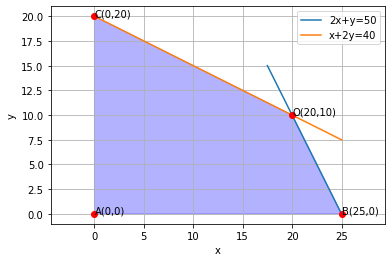
\includegraphics[width=\columnwidth]{solutions/su2021/2/13/Figure9.png}
\caption{Graphical Solution}
\label{opt/13/fig: Graphical Solution}	
\end{figure}

    

\end{enumerate}
\item Show that points A=\myvec{a&b+c}, B=\myvec{b&c+a}, C=\myvec{c&a+b} are collinear.
\\
\solution 
From theory, we understand that using dot product we can find the angle between the lines 
\begin{enumerate}
	\item 
	\begin{align}\label{eq:solutions/line_plane/74/codes:5}
		\frac{x-2}{2} = \frac{y-1}{5} &= \frac{z+3}{-3}, 
	\end{align}
	\begin{align}\label{eq:solutions/line_plane/74/codes:6}
		\frac{x+2}{-1} = \frac{y-4}{8} &= \frac{z-5}{4} 
	\end{align}


The above symmetric equations \ref{eq:solutions/line_plane/74/codes:5}, \ref{eq:solutions/line_plane/74/codes:6} can be represented in the vector form as 
\begin{align}\label{eq:solutions/line_plane/74/codes7}
	\quad \vec{r_1} &= \myvec{2\\1\\-3} + \lambda_1\myvec{2\\5\\-3}
	\\
	\quad \vec{r_2} &= \myvec{-2\\4\\5} + \lambda_2\myvec{-1\\8\\4}
\end{align}

As we have to find the angle between the vectors, we will only be taking the direction vectors into consideration. The direction vectors are $\vec{u}$ = $\myvec{2\\5\\-3}$ and $\vec{v}$ = $\myvec{-1\\8\\4}$. We can find the corresponding magnitude values

\begin{align}\label{eq:solutions/line_plane/74/codes9}
	\norm{\vec{u}} =\sqrt{2^{2}+5^{2}+(-3)^{2}} =\sqrt{38}
\end{align}
\begin{align}\label{eq:solutions/line_plane/74/codes10}
	\norm{\vec{v}} =\sqrt{(-1)^{2}+8^{2}+4^{2}} =\sqrt{81}
\end{align}

Using \ref{eq:solutions/line_plane/74/codes4}, \ref{eq:solutions/line_plane/74/codes9}, \ref{eq:solutions/line_plane/74/codes10} we get
\begin{align}
	\theta = \cos ^{-1}\frac{\myvec{2\\5\\-3}^{T}\myvec{-1\\8\\4}}{(\sqrt{38})(\sqrt{81})} 
	\\
	\theta = \cos ^{-1}\frac{26}{55.4797}
	\\
	\theta = \cos ^{-1} (0.4686)
	\\
	\theta = 62.053\degree
\end{align}

Therefore, the angle between the two lines is $62.053\degree$.See Fig. \ref{fig:solutions/line_plane/74/codesline_equation_1}

\begin{figure}
	\centering
	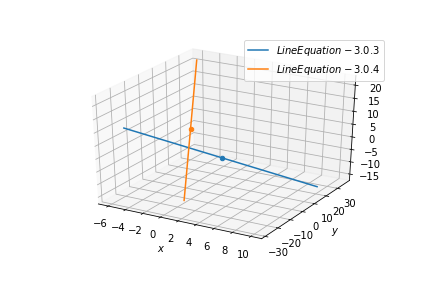
\includegraphics[width=\columnwidth]{./solutions/line_plane/74/codes/figs/Line_interest_1.png}
	\caption{Graph for equations \ref{eq:solutions/line_plane/74/codes7}}
	\label{fig:solutions/line_plane/74/codesline_equation_1}
\end{figure}


	\item 
	\begin{align}\label{eq:solutions/line_plane/74/codes12}
		\frac{x}{2} = \frac{y}{2} &= \frac{z}{1}, 
	\end{align}
	\begin{align}\label{eq:solutions/line_plane/74/codes13}
		\frac{x-5}{4} = \frac{y-2}{1} &= \frac{z-3}{8} 
	\end{align}



The above symmetric equations \ref{eq:solutions/line_plane/74/codes12}, \ref{eq:solutions/line_plane/74/codes13} can be represented in the vector form as 
\begin{align}\label{eq:solutions/line_plane/74/codes14}
	\quad \vec{r_1} &= \myvec{0\\0\\0} + \lambda_1\myvec{2\\2\\1}
	\\
	\quad \vec{r_2} &= \myvec{5\\2\\3} + \lambda_2\myvec{4\\1\\8}
\end{align}

As we have to find the angle between the vectors, we will only be taking the direction vectors into consideration. The direction vectors are $\vec{u}$ = $\myvec{2\\2\\1}$ and $\vec{v}$ = $\myvec{4\\1\\8}$. We can find the corresponding magnitude values

\begin{align}\label{eq:solutions/line_plane/74/codes16}
	\norm{\vec{u}} =\sqrt{2^{2}+2^{2}+1^{2}} =\sqrt{9}
\end{align}
\begin{align}\label{eq:solutions/line_plane/74/codes17}
	\norm{\vec{v}} =\sqrt{4^{2}+1^{2}+8^{2}} =\sqrt{81}
\end{align}

Using \ref{eq:solutions/line_plane/74/codes4}, \ref{eq:solutions/line_plane/74/codes16}, \ref{eq:solutions/line_plane/74/codes17} we get
\begin{align}
	\theta = \cos ^{-1}\frac{\myvec{2\\2\\1}^{T}\myvec{4\\1\\8}}{(\sqrt{9})(\sqrt{81})} 
	\\
	\theta = \cos ^{-1}\frac{18}{27.00}
	\\
	\theta = \cos ^{-1} (0.667)
	\\
	\theta = 48.189\degree
\end{align}

Therefore, the angle between the two lines is $48.189\degree$. See Fig. \ref{fig:solutions/line_plane/74/codesline_equation_2}


\begin{figure}
	\centering
	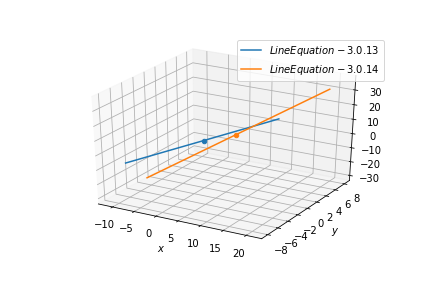
\includegraphics[width=\columnwidth]{./solutions/line_plane/74/codes/figs/Line_interest_2.png}
	\caption{Graph for equations \ref{eq:solutions/line_plane/74/codes14}}
	\label{fig:solutions/line_plane/74/codesline_equation_2}
\end{figure}
\end{enumerate}

    

\item Find values of k if area of triangle is 4sq.units and vertices are \\
(i)) \myvec{k&0}, \myvec{4&0}, \myvec{0&2} \\ (ii) \myvec{-2&0}, \myvec{0&4}, \myvec{0&k}
\item Find equation of line joining
\begin{enumerate}
\item  \myvec{1&2} and \myvec{3&6} 
\item \myvec{3&1} and \myvec{9&3}.
\end{enumerate}
\solution
\begin{enumerate}
    \item From the given information, 
\begin{align}
    \frac{AE}{EC} =  \frac{AD}{DB}&=\frac{1}{3}
\end{align}
and $\vec{D}$ divides AB in the ratio $1:3$ internally. $\vec{E}$ divides AE in the ratio $1:3$ internally.  Hence, 
\begin{align}
    \implies \vec{D} &=\frac{3\vec{A}+\vec{B}}{4}\\
    &=\myvec{\frac{13}{4}\\[2em]\frac{23}{4}}\\
    \vec{E} &=\frac{3\vec{A}+\vec{C}}{4}\\
    &=\myvec{\frac{19}{4}\\[2em]\frac{20}{4}}
\end{align}
\begin{align}
    \text{Area of } \triangle ABC &= \frac{1}{2}\norm{\brak{\vec{B-A}} \times \brak{\vec{C-A}}}\\
    &=\frac{1}{2}\norm{\myvec{-3\\-1}\times \myvec{3\\-4}}\\
        &=\frac{1}{2}\begin{vmatrix}
    -3&3\\
    -1&-4
    \end{vmatrix}\\
    &=\frac{1}{2}\sbrak{\brak{-3\times -4}-\brak{-1 \times 3}}\\
    &=\frac{15}{2}
\end{align}
\begin{align}
    \text{Area of } \triangle ADE &= \frac{1}{2}\norm{\brak{\vec{D-A}} \times \brak{\vec{E-A}}}\\
    &=\frac{1}{2}\norm{\myvec{\frac{-3}{4}\\[2em]\frac{-1}{4}}\times \myvec{\frac{3}{4}\\[2em]\frac{-4}{4}}}\\
    &=\frac{1}{2}\begin{vmatrix}
    \frac{-3}{4}&\frac{3}{4}\\[2em]
    \frac{-1}{4}&\frac{-4}{4}
    \end{vmatrix}\\
    &=\frac{1}{2}\sbrak{\brak{\frac{-3}{4}\times \frac{-4}{4}}-\brak{\frac{-1}{4} \times \frac{3}{4}}}\\
    &=\frac{15}{2\times16}
\end{align}
\begin{align}
    \frac{\text{area of } \triangle ADE}{\text{area of } \triangle ABC}=\frac{1}{16}
\end{align}
See Fig. \ref{aug/2/1plot}.
\begin{figure}[!h]
 \centering
 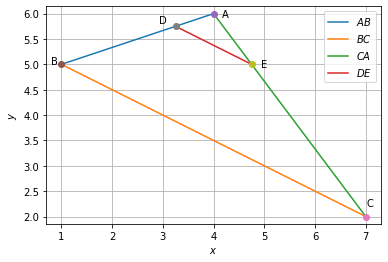
\includegraphics[width=\columnwidth]{solutions/aug/2/1/figs/figs.png}
 \caption{Plot of the triangles}
 \label{aug/2/1plot}
\end{figure}



    \item Let 
	\begin{align}
	 \vec{A} = \myvec{1\\2} , \vec{B} = \myvec{3 \\ 6}
	\end{align}
The direction vector 
\begin{align}
\vec{m}&= \vec{B}-\vec{A}=\myvec{2\\4}
\\
\implies 
    \vec{n}&= \myvec{-4\\2}
\end{align}
and 
\begin{align}
    c = \vec{n}^\top \vec {A} = \myvec{-4&2} \myvec{1\\2}=0 
\end{align}
This is verified in Fig. \ref{aug/76/2/fig:1}.
\begin{figure}[!ht]
\centering
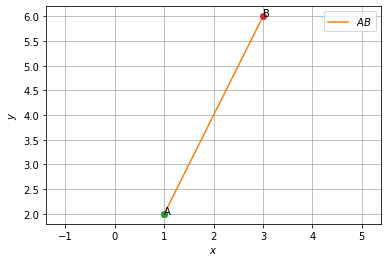
\includegraphics[width=\columnwidth]{solutions/aug/1/76/2/fig5.png}
\caption{LINE AB}
\label{aug/76/2/fig:1}
\end{figure}

    
\end{enumerate}

\item If the area of triangle is 35 sq.units with vertices \myvec{2&-6}, \myvec{5&4} and \myvec{k&4}.then k is 
\begin{enumerate}
\item 12
\item -2
\item -12,-2
\item 12,-2
\end{enumerate}
\solution
Let
\begin{align}
   \vec{A} = \myvec{2\\-6} , \vec{B} = \myvec{5 \\ 4}, \vec{C} = \myvec{k\\4} 
\end{align}
From the given information,
%
\begin{align}
   \frac{1}{2}\myvec{1 & 1& 1 \\
   \vec{A}&\vec{B}&\vec{C}}
   &= \mydet{
    1 & 1 & 1 \\ 
    2 & 5 & k \\ 
    -6 & 4 & 4} \\ &= 35
\end{align}
Simplifying the determinant, 
\begin{align}
   \mydet{1 & 1 & 1  \\ 
 2 & 5 & k \\ 
-6 & 4 & 4}
\xleftrightarrow [C_2-C_3\rightarrow C_2]{C_1-C_3\rightarrow C_1}
 \mydet{0 & 0 & 1  \\ 
 2-k & 5-k & k \\ 
10 & 0 & 4}
\end{align}
which upon expanding the cofactor yields
\begin{align}
     \mydet{2-k & 5-k \\ 
10 & 0 } = 10(5-k)
\end{align}
Thus, 
\begin{align}
   \frac{1}{2}10(5-k) &= 35
\\
  \implies  k &= -2
\end{align}

\textbf{Write Minors and Coafactors of the elements of following determinants:}
\item (i) $\begin{vmatrix}
2&-4 \\ 0 &3 \end{vmatrix}$ \\
(ii) $\begin{vmatrix}a&c \\ b &d\end{vmatrix}$
\item (i) $\begin{vmatrix}1&0&0 \\ 0&1&0 \\ 0&0&1\end{vmatrix}$\\
(ii) $\begin{vmatrix}1&0&4 \\ 3&5&-1 \\ 0&1&2\end{vmatrix}$
\item Using Cofactors of elements of second row,evaluate $\Delta$ =
$\begin{vmatrix} 5&3&8 \\ 2&0&1 \\ 1&2&3 \end{vmatrix}.$
\item Using Cofactors of elements of third column ,evaluate $\Delta$ = 
$\begin{vmatrix} 1&x&yz \\ 1&y&zx \\ 1&z&xy \end{vmatrix}.$
\item If $\Delta = \begin{vmatrix}
a_{11}&a_{12}&a_{13} \\ a_{21}&a_{22}&a_{23} \\ a_{31}&a_{32}&a_{33}
\end{vmatrix}$ and $A_{ij}$ is Cofactors of $a_{ij}$ then value of $\Delta$ is given by 
\begin{enumerate}
\item $a_{11}A_{31}+a_{12}A_{32}+a_{13}A_{33}$
\item $a_{11}A_{11}+a_{12}A_{21}+a_{13}A_{31}$
\item $a_{21}A_{11}+a_{22}A_{12}+a_{23}A_{13}$
\item $a_{11}A_{11}+a_{21}A_{21}+a_{31}A_{31}$
\end{enumerate} 
\textbf{Find adjoint of each of the matrices} 
\item $\begin{bmatrix}
1&2 \\ 3&4
\end{bmatrix}$
\item $\begin{bmatrix}
1&-1&2 \\ 2&3&5 \\ -2&0&1
\end{bmatrix}$
Verify A(adjA)=(adjA)A=$\abs{A}I$
\item $\begin{bmatrix}
2&3 \\ -4&-6
\end{bmatrix}$
\item $\begin{bmatrix}
1&-1&2 \\ 3&0&-2 \\ 1&0&3
\end{bmatrix}$
\item $\begin{bmatrix}
2&-2 \\ 4&3
\end{bmatrix}$
\item $\begin{bmatrix}
-1&5 \\ -3&2
\end{bmatrix}$
\item $\begin{bmatrix}
1&2&3 \\ 0&2&4 \\ 0&0&5
\end{bmatrix}$
\item $\begin{bmatrix}
1&0&0 \\ 3&3&0 \\ 5&2&-1
\end{bmatrix}$
\item $\begin{bmatrix}
2&1&3 \\ 4&-1&0 \\ -7&2&1
\end{bmatrix}$
\item $\begin{bmatrix}
1&-1&2 \\ 0&2&-3 \\ 3&-2&4
\end{bmatrix}$
\item $\begin{bmatrix}
1&0&0 \\ 0& \cos\alpha &\sin\alpha \\ 0&\sin\alpha&-\cos\alpha
\end{bmatrix}$
\item Let A=
$\begin{bmatrix}
3&7 \\ 2&5
\end{bmatrix}$ and B=
$\begin{bmatrix}
6&8 \\ 7&9
\end{bmatrix}.$ Verify that $(AB)^{-1}=B^{-1} A^{-1}$
\item Let A =$\begin{bmatrix}
3&1 \\ -1&2
\end{bmatrix},$ show that $A^2-5A+7I=O.$ Hence find $A^{-1}$
\solution 
From theory, we understand that using dot product we can find the angle between the lines 
\begin{enumerate}
	\item 
	\begin{align}\label{eq:solutions/line_plane/74/codes:5}
		\frac{x-2}{2} = \frac{y-1}{5} &= \frac{z+3}{-3}, 
	\end{align}
	\begin{align}\label{eq:solutions/line_plane/74/codes:6}
		\frac{x+2}{-1} = \frac{y-4}{8} &= \frac{z-5}{4} 
	\end{align}


The above symmetric equations \ref{eq:solutions/line_plane/74/codes:5}, \ref{eq:solutions/line_plane/74/codes:6} can be represented in the vector form as 
\begin{align}\label{eq:solutions/line_plane/74/codes7}
	\quad \vec{r_1} &= \myvec{2\\1\\-3} + \lambda_1\myvec{2\\5\\-3}
	\\
	\quad \vec{r_2} &= \myvec{-2\\4\\5} + \lambda_2\myvec{-1\\8\\4}
\end{align}

As we have to find the angle between the vectors, we will only be taking the direction vectors into consideration. The direction vectors are $\vec{u}$ = $\myvec{2\\5\\-3}$ and $\vec{v}$ = $\myvec{-1\\8\\4}$. We can find the corresponding magnitude values

\begin{align}\label{eq:solutions/line_plane/74/codes9}
	\norm{\vec{u}} =\sqrt{2^{2}+5^{2}+(-3)^{2}} =\sqrt{38}
\end{align}
\begin{align}\label{eq:solutions/line_plane/74/codes10}
	\norm{\vec{v}} =\sqrt{(-1)^{2}+8^{2}+4^{2}} =\sqrt{81}
\end{align}

Using \ref{eq:solutions/line_plane/74/codes4}, \ref{eq:solutions/line_plane/74/codes9}, \ref{eq:solutions/line_plane/74/codes10} we get
\begin{align}
	\theta = \cos ^{-1}\frac{\myvec{2\\5\\-3}^{T}\myvec{-1\\8\\4}}{(\sqrt{38})(\sqrt{81})} 
	\\
	\theta = \cos ^{-1}\frac{26}{55.4797}
	\\
	\theta = \cos ^{-1} (0.4686)
	\\
	\theta = 62.053\degree
\end{align}

Therefore, the angle between the two lines is $62.053\degree$.See Fig. \ref{fig:solutions/line_plane/74/codesline_equation_1}

\begin{figure}
	\centering
	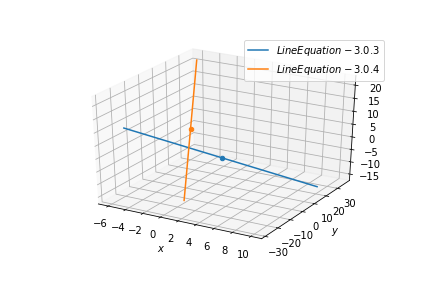
\includegraphics[width=\columnwidth]{./solutions/line_plane/74/codes/figs/Line_interest_1.png}
	\caption{Graph for equations \ref{eq:solutions/line_plane/74/codes7}}
	\label{fig:solutions/line_plane/74/codesline_equation_1}
\end{figure}


	\item 
	\begin{align}\label{eq:solutions/line_plane/74/codes12}
		\frac{x}{2} = \frac{y}{2} &= \frac{z}{1}, 
	\end{align}
	\begin{align}\label{eq:solutions/line_plane/74/codes13}
		\frac{x-5}{4} = \frac{y-2}{1} &= \frac{z-3}{8} 
	\end{align}



The above symmetric equations \ref{eq:solutions/line_plane/74/codes12}, \ref{eq:solutions/line_plane/74/codes13} can be represented in the vector form as 
\begin{align}\label{eq:solutions/line_plane/74/codes14}
	\quad \vec{r_1} &= \myvec{0\\0\\0} + \lambda_1\myvec{2\\2\\1}
	\\
	\quad \vec{r_2} &= \myvec{5\\2\\3} + \lambda_2\myvec{4\\1\\8}
\end{align}

As we have to find the angle between the vectors, we will only be taking the direction vectors into consideration. The direction vectors are $\vec{u}$ = $\myvec{2\\2\\1}$ and $\vec{v}$ = $\myvec{4\\1\\8}$. We can find the corresponding magnitude values

\begin{align}\label{eq:solutions/line_plane/74/codes16}
	\norm{\vec{u}} =\sqrt{2^{2}+2^{2}+1^{2}} =\sqrt{9}
\end{align}
\begin{align}\label{eq:solutions/line_plane/74/codes17}
	\norm{\vec{v}} =\sqrt{4^{2}+1^{2}+8^{2}} =\sqrt{81}
\end{align}

Using \ref{eq:solutions/line_plane/74/codes4}, \ref{eq:solutions/line_plane/74/codes16}, \ref{eq:solutions/line_plane/74/codes17} we get
\begin{align}
	\theta = \cos ^{-1}\frac{\myvec{2\\2\\1}^{T}\myvec{4\\1\\8}}{(\sqrt{9})(\sqrt{81})} 
	\\
	\theta = \cos ^{-1}\frac{18}{27.00}
	\\
	\theta = \cos ^{-1} (0.667)
	\\
	\theta = 48.189\degree
\end{align}

Therefore, the angle between the two lines is $48.189\degree$. See Fig. \ref{fig:solutions/line_plane/74/codesline_equation_2}


\begin{figure}
	\centering
	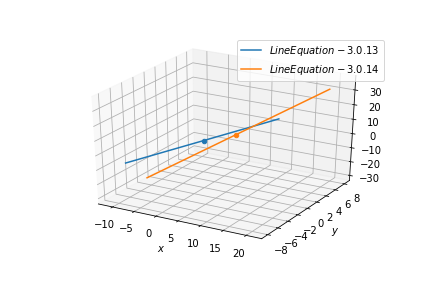
\includegraphics[width=\columnwidth]{./solutions/line_plane/74/codes/figs/Line_interest_2.png}
	\caption{Graph for equations \ref{eq:solutions/line_plane/74/codes14}}
	\label{fig:solutions/line_plane/74/codesline_equation_2}
\end{figure}
\end{enumerate}

    

\item For the matrix A= $\begin{bmatrix}
3&2 \\ 1&1
\end{bmatrix},$ find the numbers a and b such that $A^2+aA+bI=O.$
\\
\solution 
From theory, we understand that using dot product we can find the angle between the lines 
\begin{enumerate}
	\item 
	\begin{align}\label{eq:solutions/line_plane/74/codes:5}
		\frac{x-2}{2} = \frac{y-1}{5} &= \frac{z+3}{-3}, 
	\end{align}
	\begin{align}\label{eq:solutions/line_plane/74/codes:6}
		\frac{x+2}{-1} = \frac{y-4}{8} &= \frac{z-5}{4} 
	\end{align}


The above symmetric equations \ref{eq:solutions/line_plane/74/codes:5}, \ref{eq:solutions/line_plane/74/codes:6} can be represented in the vector form as 
\begin{align}\label{eq:solutions/line_plane/74/codes7}
	\quad \vec{r_1} &= \myvec{2\\1\\-3} + \lambda_1\myvec{2\\5\\-3}
	\\
	\quad \vec{r_2} &= \myvec{-2\\4\\5} + \lambda_2\myvec{-1\\8\\4}
\end{align}

As we have to find the angle between the vectors, we will only be taking the direction vectors into consideration. The direction vectors are $\vec{u}$ = $\myvec{2\\5\\-3}$ and $\vec{v}$ = $\myvec{-1\\8\\4}$. We can find the corresponding magnitude values

\begin{align}\label{eq:solutions/line_plane/74/codes9}
	\norm{\vec{u}} =\sqrt{2^{2}+5^{2}+(-3)^{2}} =\sqrt{38}
\end{align}
\begin{align}\label{eq:solutions/line_plane/74/codes10}
	\norm{\vec{v}} =\sqrt{(-1)^{2}+8^{2}+4^{2}} =\sqrt{81}
\end{align}

Using \ref{eq:solutions/line_plane/74/codes4}, \ref{eq:solutions/line_plane/74/codes9}, \ref{eq:solutions/line_plane/74/codes10} we get
\begin{align}
	\theta = \cos ^{-1}\frac{\myvec{2\\5\\-3}^{T}\myvec{-1\\8\\4}}{(\sqrt{38})(\sqrt{81})} 
	\\
	\theta = \cos ^{-1}\frac{26}{55.4797}
	\\
	\theta = \cos ^{-1} (0.4686)
	\\
	\theta = 62.053\degree
\end{align}

Therefore, the angle between the two lines is $62.053\degree$.See Fig. \ref{fig:solutions/line_plane/74/codesline_equation_1}

\begin{figure}
	\centering
	\includegraphics[width=\columnwidth]{./solutions/line_plane/74/codes/figs/Line_interest_1.png}
	\caption{Graph for equations \ref{eq:solutions/line_plane/74/codes7}}
	\label{fig:solutions/line_plane/74/codesline_equation_1}
\end{figure}


	\item 
	\begin{align}\label{eq:solutions/line_plane/74/codes12}
		\frac{x}{2} = \frac{y}{2} &= \frac{z}{1}, 
	\end{align}
	\begin{align}\label{eq:solutions/line_plane/74/codes13}
		\frac{x-5}{4} = \frac{y-2}{1} &= \frac{z-3}{8} 
	\end{align}



The above symmetric equations \ref{eq:solutions/line_plane/74/codes12}, \ref{eq:solutions/line_plane/74/codes13} can be represented in the vector form as 
\begin{align}\label{eq:solutions/line_plane/74/codes14}
	\quad \vec{r_1} &= \myvec{0\\0\\0} + \lambda_1\myvec{2\\2\\1}
	\\
	\quad \vec{r_2} &= \myvec{5\\2\\3} + \lambda_2\myvec{4\\1\\8}
\end{align}

As we have to find the angle between the vectors, we will only be taking the direction vectors into consideration. The direction vectors are $\vec{u}$ = $\myvec{2\\2\\1}$ and $\vec{v}$ = $\myvec{4\\1\\8}$. We can find the corresponding magnitude values

\begin{align}\label{eq:solutions/line_plane/74/codes16}
	\norm{\vec{u}} =\sqrt{2^{2}+2^{2}+1^{2}} =\sqrt{9}
\end{align}
\begin{align}\label{eq:solutions/line_plane/74/codes17}
	\norm{\vec{v}} =\sqrt{4^{2}+1^{2}+8^{2}} =\sqrt{81}
\end{align}

Using \ref{eq:solutions/line_plane/74/codes4}, \ref{eq:solutions/line_plane/74/codes16}, \ref{eq:solutions/line_plane/74/codes17} we get
\begin{align}
	\theta = \cos ^{-1}\frac{\myvec{2\\2\\1}^{T}\myvec{4\\1\\8}}{(\sqrt{9})(\sqrt{81})} 
	\\
	\theta = \cos ^{-1}\frac{18}{27.00}
	\\
	\theta = \cos ^{-1} (0.667)
	\\
	\theta = 48.189\degree
\end{align}

Therefore, the angle between the two lines is $48.189\degree$. See Fig. \ref{fig:solutions/line_plane/74/codesline_equation_2}


\begin{figure}
	\centering
	\includegraphics[width=\columnwidth]{./solutions/line_plane/74/codes/figs/Line_interest_2.png}
	\caption{Graph for equations \ref{eq:solutions/line_plane/74/codes14}}
	\label{fig:solutions/line_plane/74/codesline_equation_2}
\end{figure}
\end{enumerate}

    


\item For the matrix A=$\myvec{1&1&1 \\ 1&2&-3 \\ 2&-1&3}$.Show that \begin{align}
    A^3-6A^2+5A+11I=0\label{eq:det/49/1}
\end{align} and hence find $A^{-1}$.
%\item For the matrix A=$\begin{bmatrix}
%1&1&1 \\ 1&2&-3 \\ 2&-1&3
%\end{bmatrix}$ Show that $A^3-6A^2+9A-4I=O$ and hence find $A^{-1}$
\solution 
From theory, we understand that using dot product we can find the angle between the lines 
\begin{enumerate}
	\item 
	\begin{align}\label{eq:solutions/line_plane/74/codes:5}
		\frac{x-2}{2} = \frac{y-1}{5} &= \frac{z+3}{-3}, 
	\end{align}
	\begin{align}\label{eq:solutions/line_plane/74/codes:6}
		\frac{x+2}{-1} = \frac{y-4}{8} &= \frac{z-5}{4} 
	\end{align}


The above symmetric equations \ref{eq:solutions/line_plane/74/codes:5}, \ref{eq:solutions/line_plane/74/codes:6} can be represented in the vector form as 
\begin{align}\label{eq:solutions/line_plane/74/codes7}
	\quad \vec{r_1} &= \myvec{2\\1\\-3} + \lambda_1\myvec{2\\5\\-3}
	\\
	\quad \vec{r_2} &= \myvec{-2\\4\\5} + \lambda_2\myvec{-1\\8\\4}
\end{align}

As we have to find the angle between the vectors, we will only be taking the direction vectors into consideration. The direction vectors are $\vec{u}$ = $\myvec{2\\5\\-3}$ and $\vec{v}$ = $\myvec{-1\\8\\4}$. We can find the corresponding magnitude values

\begin{align}\label{eq:solutions/line_plane/74/codes9}
	\norm{\vec{u}} =\sqrt{2^{2}+5^{2}+(-3)^{2}} =\sqrt{38}
\end{align}
\begin{align}\label{eq:solutions/line_plane/74/codes10}
	\norm{\vec{v}} =\sqrt{(-1)^{2}+8^{2}+4^{2}} =\sqrt{81}
\end{align}

Using \ref{eq:solutions/line_plane/74/codes4}, \ref{eq:solutions/line_plane/74/codes9}, \ref{eq:solutions/line_plane/74/codes10} we get
\begin{align}
	\theta = \cos ^{-1}\frac{\myvec{2\\5\\-3}^{T}\myvec{-1\\8\\4}}{(\sqrt{38})(\sqrt{81})} 
	\\
	\theta = \cos ^{-1}\frac{26}{55.4797}
	\\
	\theta = \cos ^{-1} (0.4686)
	\\
	\theta = 62.053\degree
\end{align}

Therefore, the angle between the two lines is $62.053\degree$.See Fig. \ref{fig:solutions/line_plane/74/codesline_equation_1}

\begin{figure}
	\centering
	\includegraphics[width=\columnwidth]{./solutions/line_plane/74/codes/figs/Line_interest_1.png}
	\caption{Graph for equations \ref{eq:solutions/line_plane/74/codes7}}
	\label{fig:solutions/line_plane/74/codesline_equation_1}
\end{figure}


	\item 
	\begin{align}\label{eq:solutions/line_plane/74/codes12}
		\frac{x}{2} = \frac{y}{2} &= \frac{z}{1}, 
	\end{align}
	\begin{align}\label{eq:solutions/line_plane/74/codes13}
		\frac{x-5}{4} = \frac{y-2}{1} &= \frac{z-3}{8} 
	\end{align}



The above symmetric equations \ref{eq:solutions/line_plane/74/codes12}, \ref{eq:solutions/line_plane/74/codes13} can be represented in the vector form as 
\begin{align}\label{eq:solutions/line_plane/74/codes14}
	\quad \vec{r_1} &= \myvec{0\\0\\0} + \lambda_1\myvec{2\\2\\1}
	\\
	\quad \vec{r_2} &= \myvec{5\\2\\3} + \lambda_2\myvec{4\\1\\8}
\end{align}

As we have to find the angle between the vectors, we will only be taking the direction vectors into consideration. The direction vectors are $\vec{u}$ = $\myvec{2\\2\\1}$ and $\vec{v}$ = $\myvec{4\\1\\8}$. We can find the corresponding magnitude values

\begin{align}\label{eq:solutions/line_plane/74/codes16}
	\norm{\vec{u}} =\sqrt{2^{2}+2^{2}+1^{2}} =\sqrt{9}
\end{align}
\begin{align}\label{eq:solutions/line_plane/74/codes17}
	\norm{\vec{v}} =\sqrt{4^{2}+1^{2}+8^{2}} =\sqrt{81}
\end{align}

Using \ref{eq:solutions/line_plane/74/codes4}, \ref{eq:solutions/line_plane/74/codes16}, \ref{eq:solutions/line_plane/74/codes17} we get
\begin{align}
	\theta = \cos ^{-1}\frac{\myvec{2\\2\\1}^{T}\myvec{4\\1\\8}}{(\sqrt{9})(\sqrt{81})} 
	\\
	\theta = \cos ^{-1}\frac{18}{27.00}
	\\
	\theta = \cos ^{-1} (0.667)
	\\
	\theta = 48.189\degree
\end{align}

Therefore, the angle between the two lines is $48.189\degree$. See Fig. \ref{fig:solutions/line_plane/74/codesline_equation_2}


\begin{figure}
	\centering
	\includegraphics[width=\columnwidth]{./solutions/line_plane/74/codes/figs/Line_interest_2.png}
	\caption{Graph for equations \ref{eq:solutions/line_plane/74/codes14}}
	\label{fig:solutions/line_plane/74/codesline_equation_2}
\end{figure}
\end{enumerate}

    

\item Let A be a nonsingular square matrix of order 3X3 .Then $\abs{adjA}$ is equal to 
\begin{enumerate}
\item $\abs{A}$
\item $\abs{A}^2$
\item $\abs{A}^3$
\item $3\abs{A}$
\end{enumerate}
\item If A is an invertible matrix of order 2, then det($A^{-1}$) is equal to 
\begin{enumerate}
\item det(A)
\item $\frac{1}{det(A)}$
\item 1
\item 0
\end{enumerate}
\textbf{Examine the consistency of the system of given Equations.}
\item $\begin{alignedat}[t]{2}
x+3y&=5 
\\
2x+6y&=8 
\end{alignedat}$\\
\\
\solution 
From theory, we understand that using dot product we can find the angle between the lines 
\begin{enumerate}
	\item 
	\begin{align}\label{eq:solutions/line_plane/74/codes:5}
		\frac{x-2}{2} = \frac{y-1}{5} &= \frac{z+3}{-3}, 
	\end{align}
	\begin{align}\label{eq:solutions/line_plane/74/codes:6}
		\frac{x+2}{-1} = \frac{y-4}{8} &= \frac{z-5}{4} 
	\end{align}


The above symmetric equations \ref{eq:solutions/line_plane/74/codes:5}, \ref{eq:solutions/line_plane/74/codes:6} can be represented in the vector form as 
\begin{align}\label{eq:solutions/line_plane/74/codes7}
	\quad \vec{r_1} &= \myvec{2\\1\\-3} + \lambda_1\myvec{2\\5\\-3}
	\\
	\quad \vec{r_2} &= \myvec{-2\\4\\5} + \lambda_2\myvec{-1\\8\\4}
\end{align}

As we have to find the angle between the vectors, we will only be taking the direction vectors into consideration. The direction vectors are $\vec{u}$ = $\myvec{2\\5\\-3}$ and $\vec{v}$ = $\myvec{-1\\8\\4}$. We can find the corresponding magnitude values

\begin{align}\label{eq:solutions/line_plane/74/codes9}
	\norm{\vec{u}} =\sqrt{2^{2}+5^{2}+(-3)^{2}} =\sqrt{38}
\end{align}
\begin{align}\label{eq:solutions/line_plane/74/codes10}
	\norm{\vec{v}} =\sqrt{(-1)^{2}+8^{2}+4^{2}} =\sqrt{81}
\end{align}

Using \ref{eq:solutions/line_plane/74/codes4}, \ref{eq:solutions/line_plane/74/codes9}, \ref{eq:solutions/line_plane/74/codes10} we get
\begin{align}
	\theta = \cos ^{-1}\frac{\myvec{2\\5\\-3}^{T}\myvec{-1\\8\\4}}{(\sqrt{38})(\sqrt{81})} 
	\\
	\theta = \cos ^{-1}\frac{26}{55.4797}
	\\
	\theta = \cos ^{-1} (0.4686)
	\\
	\theta = 62.053\degree
\end{align}

Therefore, the angle between the two lines is $62.053\degree$.See Fig. \ref{fig:solutions/line_plane/74/codesline_equation_1}

\begin{figure}
	\centering
	\includegraphics[width=\columnwidth]{./solutions/line_plane/74/codes/figs/Line_interest_1.png}
	\caption{Graph for equations \ref{eq:solutions/line_plane/74/codes7}}
	\label{fig:solutions/line_plane/74/codesline_equation_1}
\end{figure}


	\item 
	\begin{align}\label{eq:solutions/line_plane/74/codes12}
		\frac{x}{2} = \frac{y}{2} &= \frac{z}{1}, 
	\end{align}
	\begin{align}\label{eq:solutions/line_plane/74/codes13}
		\frac{x-5}{4} = \frac{y-2}{1} &= \frac{z-3}{8} 
	\end{align}



The above symmetric equations \ref{eq:solutions/line_plane/74/codes12}, \ref{eq:solutions/line_plane/74/codes13} can be represented in the vector form as 
\begin{align}\label{eq:solutions/line_plane/74/codes14}
	\quad \vec{r_1} &= \myvec{0\\0\\0} + \lambda_1\myvec{2\\2\\1}
	\\
	\quad \vec{r_2} &= \myvec{5\\2\\3} + \lambda_2\myvec{4\\1\\8}
\end{align}

As we have to find the angle between the vectors, we will only be taking the direction vectors into consideration. The direction vectors are $\vec{u}$ = $\myvec{2\\2\\1}$ and $\vec{v}$ = $\myvec{4\\1\\8}$. We can find the corresponding magnitude values

\begin{align}\label{eq:solutions/line_plane/74/codes16}
	\norm{\vec{u}} =\sqrt{2^{2}+2^{2}+1^{2}} =\sqrt{9}
\end{align}
\begin{align}\label{eq:solutions/line_plane/74/codes17}
	\norm{\vec{v}} =\sqrt{4^{2}+1^{2}+8^{2}} =\sqrt{81}
\end{align}

Using \ref{eq:solutions/line_plane/74/codes4}, \ref{eq:solutions/line_plane/74/codes16}, \ref{eq:solutions/line_plane/74/codes17} we get
\begin{align}
	\theta = \cos ^{-1}\frac{\myvec{2\\2\\1}^{T}\myvec{4\\1\\8}}{(\sqrt{9})(\sqrt{81})} 
	\\
	\theta = \cos ^{-1}\frac{18}{27.00}
	\\
	\theta = \cos ^{-1} (0.667)
	\\
	\theta = 48.189\degree
\end{align}

Therefore, the angle between the two lines is $48.189\degree$. See Fig. \ref{fig:solutions/line_plane/74/codesline_equation_2}


\begin{figure}
	\centering
	\includegraphics[width=\columnwidth]{./solutions/line_plane/74/codes/figs/Line_interest_2.png}
	\caption{Graph for equations \ref{eq:solutions/line_plane/74/codes14}}
	\label{fig:solutions/line_plane/74/codesline_equation_2}
\end{figure}
\end{enumerate}

    

\item x+y+z=1\\ 2x+3y+2z=2\\ax+ay+2az=4\\
\\
\solution 
From theory, we understand that using dot product we can find the angle between the lines 
\begin{enumerate}
	\item 
	\begin{align}\label{eq:solutions/line_plane/74/codes:5}
		\frac{x-2}{2} = \frac{y-1}{5} &= \frac{z+3}{-3}, 
	\end{align}
	\begin{align}\label{eq:solutions/line_plane/74/codes:6}
		\frac{x+2}{-1} = \frac{y-4}{8} &= \frac{z-5}{4} 
	\end{align}


The above symmetric equations \ref{eq:solutions/line_plane/74/codes:5}, \ref{eq:solutions/line_plane/74/codes:6} can be represented in the vector form as 
\begin{align}\label{eq:solutions/line_plane/74/codes7}
	\quad \vec{r_1} &= \myvec{2\\1\\-3} + \lambda_1\myvec{2\\5\\-3}
	\\
	\quad \vec{r_2} &= \myvec{-2\\4\\5} + \lambda_2\myvec{-1\\8\\4}
\end{align}

As we have to find the angle between the vectors, we will only be taking the direction vectors into consideration. The direction vectors are $\vec{u}$ = $\myvec{2\\5\\-3}$ and $\vec{v}$ = $\myvec{-1\\8\\4}$. We can find the corresponding magnitude values

\begin{align}\label{eq:solutions/line_plane/74/codes9}
	\norm{\vec{u}} =\sqrt{2^{2}+5^{2}+(-3)^{2}} =\sqrt{38}
\end{align}
\begin{align}\label{eq:solutions/line_plane/74/codes10}
	\norm{\vec{v}} =\sqrt{(-1)^{2}+8^{2}+4^{2}} =\sqrt{81}
\end{align}

Using \ref{eq:solutions/line_plane/74/codes4}, \ref{eq:solutions/line_plane/74/codes9}, \ref{eq:solutions/line_plane/74/codes10} we get
\begin{align}
	\theta = \cos ^{-1}\frac{\myvec{2\\5\\-3}^{T}\myvec{-1\\8\\4}}{(\sqrt{38})(\sqrt{81})} 
	\\
	\theta = \cos ^{-1}\frac{26}{55.4797}
	\\
	\theta = \cos ^{-1} (0.4686)
	\\
	\theta = 62.053\degree
\end{align}

Therefore, the angle between the two lines is $62.053\degree$.See Fig. \ref{fig:solutions/line_plane/74/codesline_equation_1}

\begin{figure}
	\centering
	\includegraphics[width=\columnwidth]{./solutions/line_plane/74/codes/figs/Line_interest_1.png}
	\caption{Graph for equations \ref{eq:solutions/line_plane/74/codes7}}
	\label{fig:solutions/line_plane/74/codesline_equation_1}
\end{figure}


	\item 
	\begin{align}\label{eq:solutions/line_plane/74/codes12}
		\frac{x}{2} = \frac{y}{2} &= \frac{z}{1}, 
	\end{align}
	\begin{align}\label{eq:solutions/line_plane/74/codes13}
		\frac{x-5}{4} = \frac{y-2}{1} &= \frac{z-3}{8} 
	\end{align}



The above symmetric equations \ref{eq:solutions/line_plane/74/codes12}, \ref{eq:solutions/line_plane/74/codes13} can be represented in the vector form as 
\begin{align}\label{eq:solutions/line_plane/74/codes14}
	\quad \vec{r_1} &= \myvec{0\\0\\0} + \lambda_1\myvec{2\\2\\1}
	\\
	\quad \vec{r_2} &= \myvec{5\\2\\3} + \lambda_2\myvec{4\\1\\8}
\end{align}

As we have to find the angle between the vectors, we will only be taking the direction vectors into consideration. The direction vectors are $\vec{u}$ = $\myvec{2\\2\\1}$ and $\vec{v}$ = $\myvec{4\\1\\8}$. We can find the corresponding magnitude values

\begin{align}\label{eq:solutions/line_plane/74/codes16}
	\norm{\vec{u}} =\sqrt{2^{2}+2^{2}+1^{2}} =\sqrt{9}
\end{align}
\begin{align}\label{eq:solutions/line_plane/74/codes17}
	\norm{\vec{v}} =\sqrt{4^{2}+1^{2}+8^{2}} =\sqrt{81}
\end{align}

Using \ref{eq:solutions/line_plane/74/codes4}, \ref{eq:solutions/line_plane/74/codes16}, \ref{eq:solutions/line_plane/74/codes17} we get
\begin{align}
	\theta = \cos ^{-1}\frac{\myvec{2\\2\\1}^{T}\myvec{4\\1\\8}}{(\sqrt{9})(\sqrt{81})} 
	\\
	\theta = \cos ^{-1}\frac{18}{27.00}
	\\
	\theta = \cos ^{-1} (0.667)
	\\
	\theta = 48.189\degree
\end{align}

Therefore, the angle between the two lines is $48.189\degree$. See Fig. \ref{fig:solutions/line_plane/74/codesline_equation_2}


\begin{figure}
	\centering
	\includegraphics[width=\columnwidth]{./solutions/line_plane/74/codes/figs/Line_interest_2.png}
	\caption{Graph for equations \ref{eq:solutions/line_plane/74/codes14}}
	\label{fig:solutions/line_plane/74/codesline_equation_2}
\end{figure}
\end{enumerate}

    

\item 3x-y-2z=2 \\ 2y-z=-1 \\ 3x-5y=3\\
\\
\solution 
From theory, we understand that using dot product we can find the angle between the lines 
\begin{enumerate}
	\item 
	\begin{align}\label{eq:solutions/line_plane/74/codes:5}
		\frac{x-2}{2} = \frac{y-1}{5} &= \frac{z+3}{-3}, 
	\end{align}
	\begin{align}\label{eq:solutions/line_plane/74/codes:6}
		\frac{x+2}{-1} = \frac{y-4}{8} &= \frac{z-5}{4} 
	\end{align}


The above symmetric equations \ref{eq:solutions/line_plane/74/codes:5}, \ref{eq:solutions/line_plane/74/codes:6} can be represented in the vector form as 
\begin{align}\label{eq:solutions/line_plane/74/codes7}
	\quad \vec{r_1} &= \myvec{2\\1\\-3} + \lambda_1\myvec{2\\5\\-3}
	\\
	\quad \vec{r_2} &= \myvec{-2\\4\\5} + \lambda_2\myvec{-1\\8\\4}
\end{align}

As we have to find the angle between the vectors, we will only be taking the direction vectors into consideration. The direction vectors are $\vec{u}$ = $\myvec{2\\5\\-3}$ and $\vec{v}$ = $\myvec{-1\\8\\4}$. We can find the corresponding magnitude values

\begin{align}\label{eq:solutions/line_plane/74/codes9}
	\norm{\vec{u}} =\sqrt{2^{2}+5^{2}+(-3)^{2}} =\sqrt{38}
\end{align}
\begin{align}\label{eq:solutions/line_plane/74/codes10}
	\norm{\vec{v}} =\sqrt{(-1)^{2}+8^{2}+4^{2}} =\sqrt{81}
\end{align}

Using \ref{eq:solutions/line_plane/74/codes4}, \ref{eq:solutions/line_plane/74/codes9}, \ref{eq:solutions/line_plane/74/codes10} we get
\begin{align}
	\theta = \cos ^{-1}\frac{\myvec{2\\5\\-3}^{T}\myvec{-1\\8\\4}}{(\sqrt{38})(\sqrt{81})} 
	\\
	\theta = \cos ^{-1}\frac{26}{55.4797}
	\\
	\theta = \cos ^{-1} (0.4686)
	\\
	\theta = 62.053\degree
\end{align}

Therefore, the angle between the two lines is $62.053\degree$.See Fig. \ref{fig:solutions/line_plane/74/codesline_equation_1}

\begin{figure}
	\centering
	\includegraphics[width=\columnwidth]{./solutions/line_plane/74/codes/figs/Line_interest_1.png}
	\caption{Graph for equations \ref{eq:solutions/line_plane/74/codes7}}
	\label{fig:solutions/line_plane/74/codesline_equation_1}
\end{figure}


	\item 
	\begin{align}\label{eq:solutions/line_plane/74/codes12}
		\frac{x}{2} = \frac{y}{2} &= \frac{z}{1}, 
	\end{align}
	\begin{align}\label{eq:solutions/line_plane/74/codes13}
		\frac{x-5}{4} = \frac{y-2}{1} &= \frac{z-3}{8} 
	\end{align}



The above symmetric equations \ref{eq:solutions/line_plane/74/codes12}, \ref{eq:solutions/line_plane/74/codes13} can be represented in the vector form as 
\begin{align}\label{eq:solutions/line_plane/74/codes14}
	\quad \vec{r_1} &= \myvec{0\\0\\0} + \lambda_1\myvec{2\\2\\1}
	\\
	\quad \vec{r_2} &= \myvec{5\\2\\3} + \lambda_2\myvec{4\\1\\8}
\end{align}

As we have to find the angle between the vectors, we will only be taking the direction vectors into consideration. The direction vectors are $\vec{u}$ = $\myvec{2\\2\\1}$ and $\vec{v}$ = $\myvec{4\\1\\8}$. We can find the corresponding magnitude values

\begin{align}\label{eq:solutions/line_plane/74/codes16}
	\norm{\vec{u}} =\sqrt{2^{2}+2^{2}+1^{2}} =\sqrt{9}
\end{align}
\begin{align}\label{eq:solutions/line_plane/74/codes17}
	\norm{\vec{v}} =\sqrt{4^{2}+1^{2}+8^{2}} =\sqrt{81}
\end{align}

Using \ref{eq:solutions/line_plane/74/codes4}, \ref{eq:solutions/line_plane/74/codes16}, \ref{eq:solutions/line_plane/74/codes17} we get
\begin{align}
	\theta = \cos ^{-1}\frac{\myvec{2\\2\\1}^{T}\myvec{4\\1\\8}}{(\sqrt{9})(\sqrt{81})} 
	\\
	\theta = \cos ^{-1}\frac{18}{27.00}
	\\
	\theta = \cos ^{-1} (0.667)
	\\
	\theta = 48.189\degree
\end{align}

Therefore, the angle between the two lines is $48.189\degree$. See Fig. \ref{fig:solutions/line_plane/74/codesline_equation_2}


\begin{figure}
	\centering
	\includegraphics[width=\columnwidth]{./solutions/line_plane/74/codes/figs/Line_interest_2.png}
	\caption{Graph for equations \ref{eq:solutions/line_plane/74/codes14}}
	\label{fig:solutions/line_plane/74/codesline_equation_2}
\end{figure}
\end{enumerate}

    

\item 5x-y+4z=5 \\ 2x+3y+5z=2 \\ 5x-2y+6z=-1\\
\\
\solution
From theory, we understand that using dot product we can find the angle between the lines 
\begin{enumerate}
	\item 
	\begin{align}\label{eq:solutions/line_plane/74/codes:5}
		\frac{x-2}{2} = \frac{y-1}{5} &= \frac{z+3}{-3}, 
	\end{align}
	\begin{align}\label{eq:solutions/line_plane/74/codes:6}
		\frac{x+2}{-1} = \frac{y-4}{8} &= \frac{z-5}{4} 
	\end{align}


The above symmetric equations \ref{eq:solutions/line_plane/74/codes:5}, \ref{eq:solutions/line_plane/74/codes:6} can be represented in the vector form as 
\begin{align}\label{eq:solutions/line_plane/74/codes7}
	\quad \vec{r_1} &= \myvec{2\\1\\-3} + \lambda_1\myvec{2\\5\\-3}
	\\
	\quad \vec{r_2} &= \myvec{-2\\4\\5} + \lambda_2\myvec{-1\\8\\4}
\end{align}

As we have to find the angle between the vectors, we will only be taking the direction vectors into consideration. The direction vectors are $\vec{u}$ = $\myvec{2\\5\\-3}$ and $\vec{v}$ = $\myvec{-1\\8\\4}$. We can find the corresponding magnitude values

\begin{align}\label{eq:solutions/line_plane/74/codes9}
	\norm{\vec{u}} =\sqrt{2^{2}+5^{2}+(-3)^{2}} =\sqrt{38}
\end{align}
\begin{align}\label{eq:solutions/line_plane/74/codes10}
	\norm{\vec{v}} =\sqrt{(-1)^{2}+8^{2}+4^{2}} =\sqrt{81}
\end{align}

Using \ref{eq:solutions/line_plane/74/codes4}, \ref{eq:solutions/line_plane/74/codes9}, \ref{eq:solutions/line_plane/74/codes10} we get
\begin{align}
	\theta = \cos ^{-1}\frac{\myvec{2\\5\\-3}^{T}\myvec{-1\\8\\4}}{(\sqrt{38})(\sqrt{81})} 
	\\
	\theta = \cos ^{-1}\frac{26}{55.4797}
	\\
	\theta = \cos ^{-1} (0.4686)
	\\
	\theta = 62.053\degree
\end{align}

Therefore, the angle between the two lines is $62.053\degree$.See Fig. \ref{fig:solutions/line_plane/74/codesline_equation_1}

\begin{figure}
	\centering
	\includegraphics[width=\columnwidth]{./solutions/line_plane/74/codes/figs/Line_interest_1.png}
	\caption{Graph for equations \ref{eq:solutions/line_plane/74/codes7}}
	\label{fig:solutions/line_plane/74/codesline_equation_1}
\end{figure}


	\item 
	\begin{align}\label{eq:solutions/line_plane/74/codes12}
		\frac{x}{2} = \frac{y}{2} &= \frac{z}{1}, 
	\end{align}
	\begin{align}\label{eq:solutions/line_plane/74/codes13}
		\frac{x-5}{4} = \frac{y-2}{1} &= \frac{z-3}{8} 
	\end{align}



The above symmetric equations \ref{eq:solutions/line_plane/74/codes12}, \ref{eq:solutions/line_plane/74/codes13} can be represented in the vector form as 
\begin{align}\label{eq:solutions/line_plane/74/codes14}
	\quad \vec{r_1} &= \myvec{0\\0\\0} + \lambda_1\myvec{2\\2\\1}
	\\
	\quad \vec{r_2} &= \myvec{5\\2\\3} + \lambda_2\myvec{4\\1\\8}
\end{align}

As we have to find the angle between the vectors, we will only be taking the direction vectors into consideration. The direction vectors are $\vec{u}$ = $\myvec{2\\2\\1}$ and $\vec{v}$ = $\myvec{4\\1\\8}$. We can find the corresponding magnitude values

\begin{align}\label{eq:solutions/line_plane/74/codes16}
	\norm{\vec{u}} =\sqrt{2^{2}+2^{2}+1^{2}} =\sqrt{9}
\end{align}
\begin{align}\label{eq:solutions/line_plane/74/codes17}
	\norm{\vec{v}} =\sqrt{4^{2}+1^{2}+8^{2}} =\sqrt{81}
\end{align}

Using \ref{eq:solutions/line_plane/74/codes4}, \ref{eq:solutions/line_plane/74/codes16}, \ref{eq:solutions/line_plane/74/codes17} we get
\begin{align}
	\theta = \cos ^{-1}\frac{\myvec{2\\2\\1}^{T}\myvec{4\\1\\8}}{(\sqrt{9})(\sqrt{81})} 
	\\
	\theta = \cos ^{-1}\frac{18}{27.00}
	\\
	\theta = \cos ^{-1} (0.667)
	\\
	\theta = 48.189\degree
\end{align}

Therefore, the angle between the two lines is $48.189\degree$. See Fig. \ref{fig:solutions/line_plane/74/codesline_equation_2}


\begin{figure}
	\centering
	\includegraphics[width=\columnwidth]{./solutions/line_plane/74/codes/figs/Line_interest_2.png}
	\caption{Graph for equations \ref{eq:solutions/line_plane/74/codes14}}
	\label{fig:solutions/line_plane/74/codesline_equation_2}
\end{figure}
\end{enumerate}

    

Solve the system linear equations,using matrix method.
\item 
$\begin{alignedat}[t]{2}
%\myvec{5 & 2}\vec{x} &= 4
%\\ 
%\myvec{7 & 3}\vec{x} &= 5
5x+2y&=4 \\ 7x+3y&=5
\end{alignedat}$
\\
\solution
From theory, we understand that using dot product we can find the angle between the lines 
\begin{enumerate}
	\item 
	\begin{align}\label{eq:solutions/line_plane/74/codes:5}
		\frac{x-2}{2} = \frac{y-1}{5} &= \frac{z+3}{-3}, 
	\end{align}
	\begin{align}\label{eq:solutions/line_plane/74/codes:6}
		\frac{x+2}{-1} = \frac{y-4}{8} &= \frac{z-5}{4} 
	\end{align}


The above symmetric equations \ref{eq:solutions/line_plane/74/codes:5}, \ref{eq:solutions/line_plane/74/codes:6} can be represented in the vector form as 
\begin{align}\label{eq:solutions/line_plane/74/codes7}
	\quad \vec{r_1} &= \myvec{2\\1\\-3} + \lambda_1\myvec{2\\5\\-3}
	\\
	\quad \vec{r_2} &= \myvec{-2\\4\\5} + \lambda_2\myvec{-1\\8\\4}
\end{align}

As we have to find the angle between the vectors, we will only be taking the direction vectors into consideration. The direction vectors are $\vec{u}$ = $\myvec{2\\5\\-3}$ and $\vec{v}$ = $\myvec{-1\\8\\4}$. We can find the corresponding magnitude values

\begin{align}\label{eq:solutions/line_plane/74/codes9}
	\norm{\vec{u}} =\sqrt{2^{2}+5^{2}+(-3)^{2}} =\sqrt{38}
\end{align}
\begin{align}\label{eq:solutions/line_plane/74/codes10}
	\norm{\vec{v}} =\sqrt{(-1)^{2}+8^{2}+4^{2}} =\sqrt{81}
\end{align}

Using \ref{eq:solutions/line_plane/74/codes4}, \ref{eq:solutions/line_plane/74/codes9}, \ref{eq:solutions/line_plane/74/codes10} we get
\begin{align}
	\theta = \cos ^{-1}\frac{\myvec{2\\5\\-3}^{T}\myvec{-1\\8\\4}}{(\sqrt{38})(\sqrt{81})} 
	\\
	\theta = \cos ^{-1}\frac{26}{55.4797}
	\\
	\theta = \cos ^{-1} (0.4686)
	\\
	\theta = 62.053\degree
\end{align}

Therefore, the angle between the two lines is $62.053\degree$.See Fig. \ref{fig:solutions/line_plane/74/codesline_equation_1}

\begin{figure}
	\centering
	\includegraphics[width=\columnwidth]{./solutions/line_plane/74/codes/figs/Line_interest_1.png}
	\caption{Graph for equations \ref{eq:solutions/line_plane/74/codes7}}
	\label{fig:solutions/line_plane/74/codesline_equation_1}
\end{figure}


	\item 
	\begin{align}\label{eq:solutions/line_plane/74/codes12}
		\frac{x}{2} = \frac{y}{2} &= \frac{z}{1}, 
	\end{align}
	\begin{align}\label{eq:solutions/line_plane/74/codes13}
		\frac{x-5}{4} = \frac{y-2}{1} &= \frac{z-3}{8} 
	\end{align}



The above symmetric equations \ref{eq:solutions/line_plane/74/codes12}, \ref{eq:solutions/line_plane/74/codes13} can be represented in the vector form as 
\begin{align}\label{eq:solutions/line_plane/74/codes14}
	\quad \vec{r_1} &= \myvec{0\\0\\0} + \lambda_1\myvec{2\\2\\1}
	\\
	\quad \vec{r_2} &= \myvec{5\\2\\3} + \lambda_2\myvec{4\\1\\8}
\end{align}

As we have to find the angle between the vectors, we will only be taking the direction vectors into consideration. The direction vectors are $\vec{u}$ = $\myvec{2\\2\\1}$ and $\vec{v}$ = $\myvec{4\\1\\8}$. We can find the corresponding magnitude values

\begin{align}\label{eq:solutions/line_plane/74/codes16}
	\norm{\vec{u}} =\sqrt{2^{2}+2^{2}+1^{2}} =\sqrt{9}
\end{align}
\begin{align}\label{eq:solutions/line_plane/74/codes17}
	\norm{\vec{v}} =\sqrt{4^{2}+1^{2}+8^{2}} =\sqrt{81}
\end{align}

Using \ref{eq:solutions/line_plane/74/codes4}, \ref{eq:solutions/line_plane/74/codes16}, \ref{eq:solutions/line_plane/74/codes17} we get
\begin{align}
	\theta = \cos ^{-1}\frac{\myvec{2\\2\\1}^{T}\myvec{4\\1\\8}}{(\sqrt{9})(\sqrt{81})} 
	\\
	\theta = \cos ^{-1}\frac{18}{27.00}
	\\
	\theta = \cos ^{-1} (0.667)
	\\
	\theta = 48.189\degree
\end{align}

Therefore, the angle between the two lines is $48.189\degree$. See Fig. \ref{fig:solutions/line_plane/74/codesline_equation_2}


\begin{figure}
	\centering
	\includegraphics[width=\columnwidth]{./solutions/line_plane/74/codes/figs/Line_interest_2.png}
	\caption{Graph for equations \ref{eq:solutions/line_plane/74/codes14}}
	\label{fig:solutions/line_plane/74/codesline_equation_2}
\end{figure}
\end{enumerate}

    

\item 
$\begin{alignedat}[t]{2}
%\myvec{2 & -1}\vec{x} &= -2
%\\ 
%\myvec{3 & 4}\vec{x} &= 3
2x-y&=-2 \\ 3x+4y&=3
\end{alignedat}$
\\
\solution
From theory, we understand that using dot product we can find the angle between the lines 
\begin{enumerate}
	\item 
	\begin{align}\label{eq:solutions/line_plane/74/codes:5}
		\frac{x-2}{2} = \frac{y-1}{5} &= \frac{z+3}{-3}, 
	\end{align}
	\begin{align}\label{eq:solutions/line_plane/74/codes:6}
		\frac{x+2}{-1} = \frac{y-4}{8} &= \frac{z-5}{4} 
	\end{align}


The above symmetric equations \ref{eq:solutions/line_plane/74/codes:5}, \ref{eq:solutions/line_plane/74/codes:6} can be represented in the vector form as 
\begin{align}\label{eq:solutions/line_plane/74/codes7}
	\quad \vec{r_1} &= \myvec{2\\1\\-3} + \lambda_1\myvec{2\\5\\-3}
	\\
	\quad \vec{r_2} &= \myvec{-2\\4\\5} + \lambda_2\myvec{-1\\8\\4}
\end{align}

As we have to find the angle between the vectors, we will only be taking the direction vectors into consideration. The direction vectors are $\vec{u}$ = $\myvec{2\\5\\-3}$ and $\vec{v}$ = $\myvec{-1\\8\\4}$. We can find the corresponding magnitude values

\begin{align}\label{eq:solutions/line_plane/74/codes9}
	\norm{\vec{u}} =\sqrt{2^{2}+5^{2}+(-3)^{2}} =\sqrt{38}
\end{align}
\begin{align}\label{eq:solutions/line_plane/74/codes10}
	\norm{\vec{v}} =\sqrt{(-1)^{2}+8^{2}+4^{2}} =\sqrt{81}
\end{align}

Using \ref{eq:solutions/line_plane/74/codes4}, \ref{eq:solutions/line_plane/74/codes9}, \ref{eq:solutions/line_plane/74/codes10} we get
\begin{align}
	\theta = \cos ^{-1}\frac{\myvec{2\\5\\-3}^{T}\myvec{-1\\8\\4}}{(\sqrt{38})(\sqrt{81})} 
	\\
	\theta = \cos ^{-1}\frac{26}{55.4797}
	\\
	\theta = \cos ^{-1} (0.4686)
	\\
	\theta = 62.053\degree
\end{align}

Therefore, the angle between the two lines is $62.053\degree$.See Fig. \ref{fig:solutions/line_plane/74/codesline_equation_1}

\begin{figure}
	\centering
	\includegraphics[width=\columnwidth]{./solutions/line_plane/74/codes/figs/Line_interest_1.png}
	\caption{Graph for equations \ref{eq:solutions/line_plane/74/codes7}}
	\label{fig:solutions/line_plane/74/codesline_equation_1}
\end{figure}


	\item 
	\begin{align}\label{eq:solutions/line_plane/74/codes12}
		\frac{x}{2} = \frac{y}{2} &= \frac{z}{1}, 
	\end{align}
	\begin{align}\label{eq:solutions/line_plane/74/codes13}
		\frac{x-5}{4} = \frac{y-2}{1} &= \frac{z-3}{8} 
	\end{align}



The above symmetric equations \ref{eq:solutions/line_plane/74/codes12}, \ref{eq:solutions/line_plane/74/codes13} can be represented in the vector form as 
\begin{align}\label{eq:solutions/line_plane/74/codes14}
	\quad \vec{r_1} &= \myvec{0\\0\\0} + \lambda_1\myvec{2\\2\\1}
	\\
	\quad \vec{r_2} &= \myvec{5\\2\\3} + \lambda_2\myvec{4\\1\\8}
\end{align}

As we have to find the angle between the vectors, we will only be taking the direction vectors into consideration. The direction vectors are $\vec{u}$ = $\myvec{2\\2\\1}$ and $\vec{v}$ = $\myvec{4\\1\\8}$. We can find the corresponding magnitude values

\begin{align}\label{eq:solutions/line_plane/74/codes16}
	\norm{\vec{u}} =\sqrt{2^{2}+2^{2}+1^{2}} =\sqrt{9}
\end{align}
\begin{align}\label{eq:solutions/line_plane/74/codes17}
	\norm{\vec{v}} =\sqrt{4^{2}+1^{2}+8^{2}} =\sqrt{81}
\end{align}

Using \ref{eq:solutions/line_plane/74/codes4}, \ref{eq:solutions/line_plane/74/codes16}, \ref{eq:solutions/line_plane/74/codes17} we get
\begin{align}
	\theta = \cos ^{-1}\frac{\myvec{2\\2\\1}^{T}\myvec{4\\1\\8}}{(\sqrt{9})(\sqrt{81})} 
	\\
	\theta = \cos ^{-1}\frac{18}{27.00}
	\\
	\theta = \cos ^{-1} (0.667)
	\\
	\theta = 48.189\degree
\end{align}

Therefore, the angle between the two lines is $48.189\degree$. See Fig. \ref{fig:solutions/line_plane/74/codesline_equation_2}


\begin{figure}
	\centering
	\includegraphics[width=\columnwidth]{./solutions/line_plane/74/codes/figs/Line_interest_2.png}
	\caption{Graph for equations \ref{eq:solutions/line_plane/74/codes14}}
	\label{fig:solutions/line_plane/74/codesline_equation_2}
\end{figure}
\end{enumerate}

    

\item $\begin{alignedat}[t]{2}
%\myvec{4 & -3}\vec{x} &= 3
%\\ 
%\myvec{3 & -5}\vec{x} &= 7
4x-3y&=3 \\ 3x-5y&=7
\end{alignedat}$
\\
\solution
From theory, we understand that using dot product we can find the angle between the lines 
\begin{enumerate}
	\item 
	\begin{align}\label{eq:solutions/line_plane/74/codes:5}
		\frac{x-2}{2} = \frac{y-1}{5} &= \frac{z+3}{-3}, 
	\end{align}
	\begin{align}\label{eq:solutions/line_plane/74/codes:6}
		\frac{x+2}{-1} = \frac{y-4}{8} &= \frac{z-5}{4} 
	\end{align}


The above symmetric equations \ref{eq:solutions/line_plane/74/codes:5}, \ref{eq:solutions/line_plane/74/codes:6} can be represented in the vector form as 
\begin{align}\label{eq:solutions/line_plane/74/codes7}
	\quad \vec{r_1} &= \myvec{2\\1\\-3} + \lambda_1\myvec{2\\5\\-3}
	\\
	\quad \vec{r_2} &= \myvec{-2\\4\\5} + \lambda_2\myvec{-1\\8\\4}
\end{align}

As we have to find the angle between the vectors, we will only be taking the direction vectors into consideration. The direction vectors are $\vec{u}$ = $\myvec{2\\5\\-3}$ and $\vec{v}$ = $\myvec{-1\\8\\4}$. We can find the corresponding magnitude values

\begin{align}\label{eq:solutions/line_plane/74/codes9}
	\norm{\vec{u}} =\sqrt{2^{2}+5^{2}+(-3)^{2}} =\sqrt{38}
\end{align}
\begin{align}\label{eq:solutions/line_plane/74/codes10}
	\norm{\vec{v}} =\sqrt{(-1)^{2}+8^{2}+4^{2}} =\sqrt{81}
\end{align}

Using \ref{eq:solutions/line_plane/74/codes4}, \ref{eq:solutions/line_plane/74/codes9}, \ref{eq:solutions/line_plane/74/codes10} we get
\begin{align}
	\theta = \cos ^{-1}\frac{\myvec{2\\5\\-3}^{T}\myvec{-1\\8\\4}}{(\sqrt{38})(\sqrt{81})} 
	\\
	\theta = \cos ^{-1}\frac{26}{55.4797}
	\\
	\theta = \cos ^{-1} (0.4686)
	\\
	\theta = 62.053\degree
\end{align}

Therefore, the angle between the two lines is $62.053\degree$.See Fig. \ref{fig:solutions/line_plane/74/codesline_equation_1}

\begin{figure}
	\centering
	\includegraphics[width=\columnwidth]{./solutions/line_plane/74/codes/figs/Line_interest_1.png}
	\caption{Graph for equations \ref{eq:solutions/line_plane/74/codes7}}
	\label{fig:solutions/line_plane/74/codesline_equation_1}
\end{figure}


	\item 
	\begin{align}\label{eq:solutions/line_plane/74/codes12}
		\frac{x}{2} = \frac{y}{2} &= \frac{z}{1}, 
	\end{align}
	\begin{align}\label{eq:solutions/line_plane/74/codes13}
		\frac{x-5}{4} = \frac{y-2}{1} &= \frac{z-3}{8} 
	\end{align}



The above symmetric equations \ref{eq:solutions/line_plane/74/codes12}, \ref{eq:solutions/line_plane/74/codes13} can be represented in the vector form as 
\begin{align}\label{eq:solutions/line_plane/74/codes14}
	\quad \vec{r_1} &= \myvec{0\\0\\0} + \lambda_1\myvec{2\\2\\1}
	\\
	\quad \vec{r_2} &= \myvec{5\\2\\3} + \lambda_2\myvec{4\\1\\8}
\end{align}

As we have to find the angle between the vectors, we will only be taking the direction vectors into consideration. The direction vectors are $\vec{u}$ = $\myvec{2\\2\\1}$ and $\vec{v}$ = $\myvec{4\\1\\8}$. We can find the corresponding magnitude values

\begin{align}\label{eq:solutions/line_plane/74/codes16}
	\norm{\vec{u}} =\sqrt{2^{2}+2^{2}+1^{2}} =\sqrt{9}
\end{align}
\begin{align}\label{eq:solutions/line_plane/74/codes17}
	\norm{\vec{v}} =\sqrt{4^{2}+1^{2}+8^{2}} =\sqrt{81}
\end{align}

Using \ref{eq:solutions/line_plane/74/codes4}, \ref{eq:solutions/line_plane/74/codes16}, \ref{eq:solutions/line_plane/74/codes17} we get
\begin{align}
	\theta = \cos ^{-1}\frac{\myvec{2\\2\\1}^{T}\myvec{4\\1\\8}}{(\sqrt{9})(\sqrt{81})} 
	\\
	\theta = \cos ^{-1}\frac{18}{27.00}
	\\
	\theta = \cos ^{-1} (0.667)
	\\
	\theta = 48.189\degree
\end{align}

Therefore, the angle between the two lines is $48.189\degree$. See Fig. \ref{fig:solutions/line_plane/74/codesline_equation_2}


\begin{figure}
	\centering
	\includegraphics[width=\columnwidth]{./solutions/line_plane/74/codes/figs/Line_interest_2.png}
	\caption{Graph for equations \ref{eq:solutions/line_plane/74/codes14}}
	\label{fig:solutions/line_plane/74/codesline_equation_2}
\end{figure}
\end{enumerate}

    

\item $\begin{alignedat}[t]{2}
%\myvec{5 & 2}\vec{x} &= 3
%\\ 
%\myvec{3 & 2}\vec{x} &= 5
5x+2y&=3 \\ 3x+2y&=5
\end{alignedat}$\\
\\
\solution
From theory, we understand that using dot product we can find the angle between the lines 
\begin{enumerate}
	\item 
	\begin{align}\label{eq:solutions/line_plane/74/codes:5}
		\frac{x-2}{2} = \frac{y-1}{5} &= \frac{z+3}{-3}, 
	\end{align}
	\begin{align}\label{eq:solutions/line_plane/74/codes:6}
		\frac{x+2}{-1} = \frac{y-4}{8} &= \frac{z-5}{4} 
	\end{align}


The above symmetric equations \ref{eq:solutions/line_plane/74/codes:5}, \ref{eq:solutions/line_plane/74/codes:6} can be represented in the vector form as 
\begin{align}\label{eq:solutions/line_plane/74/codes7}
	\quad \vec{r_1} &= \myvec{2\\1\\-3} + \lambda_1\myvec{2\\5\\-3}
	\\
	\quad \vec{r_2} &= \myvec{-2\\4\\5} + \lambda_2\myvec{-1\\8\\4}
\end{align}

As we have to find the angle between the vectors, we will only be taking the direction vectors into consideration. The direction vectors are $\vec{u}$ = $\myvec{2\\5\\-3}$ and $\vec{v}$ = $\myvec{-1\\8\\4}$. We can find the corresponding magnitude values

\begin{align}\label{eq:solutions/line_plane/74/codes9}
	\norm{\vec{u}} =\sqrt{2^{2}+5^{2}+(-3)^{2}} =\sqrt{38}
\end{align}
\begin{align}\label{eq:solutions/line_plane/74/codes10}
	\norm{\vec{v}} =\sqrt{(-1)^{2}+8^{2}+4^{2}} =\sqrt{81}
\end{align}

Using \ref{eq:solutions/line_plane/74/codes4}, \ref{eq:solutions/line_plane/74/codes9}, \ref{eq:solutions/line_plane/74/codes10} we get
\begin{align}
	\theta = \cos ^{-1}\frac{\myvec{2\\5\\-3}^{T}\myvec{-1\\8\\4}}{(\sqrt{38})(\sqrt{81})} 
	\\
	\theta = \cos ^{-1}\frac{26}{55.4797}
	\\
	\theta = \cos ^{-1} (0.4686)
	\\
	\theta = 62.053\degree
\end{align}

Therefore, the angle between the two lines is $62.053\degree$.See Fig. \ref{fig:solutions/line_plane/74/codesline_equation_1}

\begin{figure}
	\centering
	\includegraphics[width=\columnwidth]{./solutions/line_plane/74/codes/figs/Line_interest_1.png}
	\caption{Graph for equations \ref{eq:solutions/line_plane/74/codes7}}
	\label{fig:solutions/line_plane/74/codesline_equation_1}
\end{figure}


	\item 
	\begin{align}\label{eq:solutions/line_plane/74/codes12}
		\frac{x}{2} = \frac{y}{2} &= \frac{z}{1}, 
	\end{align}
	\begin{align}\label{eq:solutions/line_plane/74/codes13}
		\frac{x-5}{4} = \frac{y-2}{1} &= \frac{z-3}{8} 
	\end{align}



The above symmetric equations \ref{eq:solutions/line_plane/74/codes12}, \ref{eq:solutions/line_plane/74/codes13} can be represented in the vector form as 
\begin{align}\label{eq:solutions/line_plane/74/codes14}
	\quad \vec{r_1} &= \myvec{0\\0\\0} + \lambda_1\myvec{2\\2\\1}
	\\
	\quad \vec{r_2} &= \myvec{5\\2\\3} + \lambda_2\myvec{4\\1\\8}
\end{align}

As we have to find the angle between the vectors, we will only be taking the direction vectors into consideration. The direction vectors are $\vec{u}$ = $\myvec{2\\2\\1}$ and $\vec{v}$ = $\myvec{4\\1\\8}$. We can find the corresponding magnitude values

\begin{align}\label{eq:solutions/line_plane/74/codes16}
	\norm{\vec{u}} =\sqrt{2^{2}+2^{2}+1^{2}} =\sqrt{9}
\end{align}
\begin{align}\label{eq:solutions/line_plane/74/codes17}
	\norm{\vec{v}} =\sqrt{4^{2}+1^{2}+8^{2}} =\sqrt{81}
\end{align}

Using \ref{eq:solutions/line_plane/74/codes4}, \ref{eq:solutions/line_plane/74/codes16}, \ref{eq:solutions/line_plane/74/codes17} we get
\begin{align}
	\theta = \cos ^{-1}\frac{\myvec{2\\2\\1}^{T}\myvec{4\\1\\8}}{(\sqrt{9})(\sqrt{81})} 
	\\
	\theta = \cos ^{-1}\frac{18}{27.00}
	\\
	\theta = \cos ^{-1} (0.667)
	\\
	\theta = 48.189\degree
\end{align}

Therefore, the angle between the two lines is $48.189\degree$. See Fig. \ref{fig:solutions/line_plane/74/codesline_equation_2}


\begin{figure}
	\centering
	\includegraphics[width=\columnwidth]{./solutions/line_plane/74/codes/figs/Line_interest_2.png}
	\caption{Graph for equations \ref{eq:solutions/line_plane/74/codes14}}
	\label{fig:solutions/line_plane/74/codesline_equation_2}
\end{figure}
\end{enumerate}

    

\item 2x+y+z = 1 \\ x-2y-z = $\frac{3}{2}$ \\ 3y- 5z = 9\\
\item x-y+z = 4 \\ 2x+y-3z = 0 \\ x+y+z = 2\\
\item 2x+3y+3z = 5 \\ x-2y+z = -4 \\ 3x-y-2z = 3\\
\item x-y+2z = 7 \\ 3x+4y-5z = -5 \\ 2x-y+3z = 12\\ 
\item If A=$\begin{bmatrix}
2&-3&5 \\ 3&2&-4 \\ 1&1&-2
\end{bmatrix},$ find $A^{-1}.$ Using $A^{-1}$ solve the system of equations \\
2x-3y+5z = 11, \\ 3x+2y-4z = -5, \\ x+y-2z =-3.\\
\item The cost of 4 kg onion, 3 kg wheat and 2 kg rice is \rupee 60. The cost of 2 kg onion,4 kg wheat and 6 kg rice is \rupee 90.The cost of 6kg onion 2kg wheat and 3kg rice is \rupee 70.Find the cost of each item per kg by matrix mathod. 
\item Prove that the determinant \\
$\begin{vmatrix}
x &\sin\theta&\cos\theta \\ -\sin\theta&-x&1 \\ \cos\theta&1&x
\end{vmatrix}$ 
is independent of $\theta$
\\
\solution 
From theory, we understand that using dot product we can find the angle between the lines 
\begin{enumerate}
	\item 
	\begin{align}\label{eq:solutions/line_plane/74/codes:5}
		\frac{x-2}{2} = \frac{y-1}{5} &= \frac{z+3}{-3}, 
	\end{align}
	\begin{align}\label{eq:solutions/line_plane/74/codes:6}
		\frac{x+2}{-1} = \frac{y-4}{8} &= \frac{z-5}{4} 
	\end{align}


The above symmetric equations \ref{eq:solutions/line_plane/74/codes:5}, \ref{eq:solutions/line_plane/74/codes:6} can be represented in the vector form as 
\begin{align}\label{eq:solutions/line_plane/74/codes7}
	\quad \vec{r_1} &= \myvec{2\\1\\-3} + \lambda_1\myvec{2\\5\\-3}
	\\
	\quad \vec{r_2} &= \myvec{-2\\4\\5} + \lambda_2\myvec{-1\\8\\4}
\end{align}

As we have to find the angle between the vectors, we will only be taking the direction vectors into consideration. The direction vectors are $\vec{u}$ = $\myvec{2\\5\\-3}$ and $\vec{v}$ = $\myvec{-1\\8\\4}$. We can find the corresponding magnitude values

\begin{align}\label{eq:solutions/line_plane/74/codes9}
	\norm{\vec{u}} =\sqrt{2^{2}+5^{2}+(-3)^{2}} =\sqrt{38}
\end{align}
\begin{align}\label{eq:solutions/line_plane/74/codes10}
	\norm{\vec{v}} =\sqrt{(-1)^{2}+8^{2}+4^{2}} =\sqrt{81}
\end{align}

Using \ref{eq:solutions/line_plane/74/codes4}, \ref{eq:solutions/line_plane/74/codes9}, \ref{eq:solutions/line_plane/74/codes10} we get
\begin{align}
	\theta = \cos ^{-1}\frac{\myvec{2\\5\\-3}^{T}\myvec{-1\\8\\4}}{(\sqrt{38})(\sqrt{81})} 
	\\
	\theta = \cos ^{-1}\frac{26}{55.4797}
	\\
	\theta = \cos ^{-1} (0.4686)
	\\
	\theta = 62.053\degree
\end{align}

Therefore, the angle between the two lines is $62.053\degree$.See Fig. \ref{fig:solutions/line_plane/74/codesline_equation_1}

\begin{figure}
	\centering
	\includegraphics[width=\columnwidth]{./solutions/line_plane/74/codes/figs/Line_interest_1.png}
	\caption{Graph for equations \ref{eq:solutions/line_plane/74/codes7}}
	\label{fig:solutions/line_plane/74/codesline_equation_1}
\end{figure}


	\item 
	\begin{align}\label{eq:solutions/line_plane/74/codes12}
		\frac{x}{2} = \frac{y}{2} &= \frac{z}{1}, 
	\end{align}
	\begin{align}\label{eq:solutions/line_plane/74/codes13}
		\frac{x-5}{4} = \frac{y-2}{1} &= \frac{z-3}{8} 
	\end{align}



The above symmetric equations \ref{eq:solutions/line_plane/74/codes12}, \ref{eq:solutions/line_plane/74/codes13} can be represented in the vector form as 
\begin{align}\label{eq:solutions/line_plane/74/codes14}
	\quad \vec{r_1} &= \myvec{0\\0\\0} + \lambda_1\myvec{2\\2\\1}
	\\
	\quad \vec{r_2} &= \myvec{5\\2\\3} + \lambda_2\myvec{4\\1\\8}
\end{align}

As we have to find the angle between the vectors, we will only be taking the direction vectors into consideration. The direction vectors are $\vec{u}$ = $\myvec{2\\2\\1}$ and $\vec{v}$ = $\myvec{4\\1\\8}$. We can find the corresponding magnitude values

\begin{align}\label{eq:solutions/line_plane/74/codes16}
	\norm{\vec{u}} =\sqrt{2^{2}+2^{2}+1^{2}} =\sqrt{9}
\end{align}
\begin{align}\label{eq:solutions/line_plane/74/codes17}
	\norm{\vec{v}} =\sqrt{4^{2}+1^{2}+8^{2}} =\sqrt{81}
\end{align}

Using \ref{eq:solutions/line_plane/74/codes4}, \ref{eq:solutions/line_plane/74/codes16}, \ref{eq:solutions/line_plane/74/codes17} we get
\begin{align}
	\theta = \cos ^{-1}\frac{\myvec{2\\2\\1}^{T}\myvec{4\\1\\8}}{(\sqrt{9})(\sqrt{81})} 
	\\
	\theta = \cos ^{-1}\frac{18}{27.00}
	\\
	\theta = \cos ^{-1} (0.667)
	\\
	\theta = 48.189\degree
\end{align}

Therefore, the angle between the two lines is $48.189\degree$. See Fig. \ref{fig:solutions/line_plane/74/codesline_equation_2}


\begin{figure}
	\centering
	\includegraphics[width=\columnwidth]{./solutions/line_plane/74/codes/figs/Line_interest_2.png}
	\caption{Graph for equations \ref{eq:solutions/line_plane/74/codes14}}
	\label{fig:solutions/line_plane/74/codesline_equation_2}
\end{figure}
\end{enumerate}

    


\item Without expanding the determinant, prove that\\ $\begin{vmatrix}
a&a^2&bc \\ b&b^2&ca \\c&c^2&ab
\end{vmatrix}=\begin{vmatrix}
1&a^2&a^3 \\ 1&b^2&b^3 \\ 1&c^2&c^3
\end{vmatrix}$.
\\
\solution
%From theory, we understand that using dot product we can find the angle between the lines 
\begin{enumerate}
	\item 
	\begin{align}\label{eq:solutions/line_plane/74/codes:5}
		\frac{x-2}{2} = \frac{y-1}{5} &= \frac{z+3}{-3}, 
	\end{align}
	\begin{align}\label{eq:solutions/line_plane/74/codes:6}
		\frac{x+2}{-1} = \frac{y-4}{8} &= \frac{z-5}{4} 
	\end{align}


The above symmetric equations \ref{eq:solutions/line_plane/74/codes:5}, \ref{eq:solutions/line_plane/74/codes:6} can be represented in the vector form as 
\begin{align}\label{eq:solutions/line_plane/74/codes7}
	\quad \vec{r_1} &= \myvec{2\\1\\-3} + \lambda_1\myvec{2\\5\\-3}
	\\
	\quad \vec{r_2} &= \myvec{-2\\4\\5} + \lambda_2\myvec{-1\\8\\4}
\end{align}

As we have to find the angle between the vectors, we will only be taking the direction vectors into consideration. The direction vectors are $\vec{u}$ = $\myvec{2\\5\\-3}$ and $\vec{v}$ = $\myvec{-1\\8\\4}$. We can find the corresponding magnitude values

\begin{align}\label{eq:solutions/line_plane/74/codes9}
	\norm{\vec{u}} =\sqrt{2^{2}+5^{2}+(-3)^{2}} =\sqrt{38}
\end{align}
\begin{align}\label{eq:solutions/line_plane/74/codes10}
	\norm{\vec{v}} =\sqrt{(-1)^{2}+8^{2}+4^{2}} =\sqrt{81}
\end{align}

Using \ref{eq:solutions/line_plane/74/codes4}, \ref{eq:solutions/line_plane/74/codes9}, \ref{eq:solutions/line_plane/74/codes10} we get
\begin{align}
	\theta = \cos ^{-1}\frac{\myvec{2\\5\\-3}^{T}\myvec{-1\\8\\4}}{(\sqrt{38})(\sqrt{81})} 
	\\
	\theta = \cos ^{-1}\frac{26}{55.4797}
	\\
	\theta = \cos ^{-1} (0.4686)
	\\
	\theta = 62.053\degree
\end{align}

Therefore, the angle between the two lines is $62.053\degree$.See Fig. \ref{fig:solutions/line_plane/74/codesline_equation_1}

\begin{figure}
	\centering
	\includegraphics[width=\columnwidth]{./solutions/line_plane/74/codes/figs/Line_interest_1.png}
	\caption{Graph for equations \ref{eq:solutions/line_plane/74/codes7}}
	\label{fig:solutions/line_plane/74/codesline_equation_1}
\end{figure}


	\item 
	\begin{align}\label{eq:solutions/line_plane/74/codes12}
		\frac{x}{2} = \frac{y}{2} &= \frac{z}{1}, 
	\end{align}
	\begin{align}\label{eq:solutions/line_plane/74/codes13}
		\frac{x-5}{4} = \frac{y-2}{1} &= \frac{z-3}{8} 
	\end{align}



The above symmetric equations \ref{eq:solutions/line_plane/74/codes12}, \ref{eq:solutions/line_plane/74/codes13} can be represented in the vector form as 
\begin{align}\label{eq:solutions/line_plane/74/codes14}
	\quad \vec{r_1} &= \myvec{0\\0\\0} + \lambda_1\myvec{2\\2\\1}
	\\
	\quad \vec{r_2} &= \myvec{5\\2\\3} + \lambda_2\myvec{4\\1\\8}
\end{align}

As we have to find the angle between the vectors, we will only be taking the direction vectors into consideration. The direction vectors are $\vec{u}$ = $\myvec{2\\2\\1}$ and $\vec{v}$ = $\myvec{4\\1\\8}$. We can find the corresponding magnitude values

\begin{align}\label{eq:solutions/line_plane/74/codes16}
	\norm{\vec{u}} =\sqrt{2^{2}+2^{2}+1^{2}} =\sqrt{9}
\end{align}
\begin{align}\label{eq:solutions/line_plane/74/codes17}
	\norm{\vec{v}} =\sqrt{4^{2}+1^{2}+8^{2}} =\sqrt{81}
\end{align}

Using \ref{eq:solutions/line_plane/74/codes4}, \ref{eq:solutions/line_plane/74/codes16}, \ref{eq:solutions/line_plane/74/codes17} we get
\begin{align}
	\theta = \cos ^{-1}\frac{\myvec{2\\2\\1}^{T}\myvec{4\\1\\8}}{(\sqrt{9})(\sqrt{81})} 
	\\
	\theta = \cos ^{-1}\frac{18}{27.00}
	\\
	\theta = \cos ^{-1} (0.667)
	\\
	\theta = 48.189\degree
\end{align}

Therefore, the angle between the two lines is $48.189\degree$. See Fig. \ref{fig:solutions/line_plane/74/codesline_equation_2}


\begin{figure}
	\centering
	\includegraphics[width=\columnwidth]{./solutions/line_plane/74/codes/figs/Line_interest_2.png}
	\caption{Graph for equations \ref{eq:solutions/line_plane/74/codes14}}
	\label{fig:solutions/line_plane/74/codesline_equation_2}
\end{figure}
\end{enumerate}

    

\item Evaluate 
$\begin{vmatrix}
\cos\alpha \cos\beta &\cos\alpha \sin\beta &-\sin\alpha \\ -\sin\beta & \cos\beta &0 \\ \sin\alpha\cos\beta&\sin\alpha\sin\beta&\cos\alpha
\end{vmatrix}.$\\
\solution 
From theory, we understand that using dot product we can find the angle between the lines 
\begin{enumerate}
	\item 
	\begin{align}\label{eq:solutions/line_plane/74/codes:5}
		\frac{x-2}{2} = \frac{y-1}{5} &= \frac{z+3}{-3}, 
	\end{align}
	\begin{align}\label{eq:solutions/line_plane/74/codes:6}
		\frac{x+2}{-1} = \frac{y-4}{8} &= \frac{z-5}{4} 
	\end{align}


The above symmetric equations \ref{eq:solutions/line_plane/74/codes:5}, \ref{eq:solutions/line_plane/74/codes:6} can be represented in the vector form as 
\begin{align}\label{eq:solutions/line_plane/74/codes7}
	\quad \vec{r_1} &= \myvec{2\\1\\-3} + \lambda_1\myvec{2\\5\\-3}
	\\
	\quad \vec{r_2} &= \myvec{-2\\4\\5} + \lambda_2\myvec{-1\\8\\4}
\end{align}

As we have to find the angle between the vectors, we will only be taking the direction vectors into consideration. The direction vectors are $\vec{u}$ = $\myvec{2\\5\\-3}$ and $\vec{v}$ = $\myvec{-1\\8\\4}$. We can find the corresponding magnitude values

\begin{align}\label{eq:solutions/line_plane/74/codes9}
	\norm{\vec{u}} =\sqrt{2^{2}+5^{2}+(-3)^{2}} =\sqrt{38}
\end{align}
\begin{align}\label{eq:solutions/line_plane/74/codes10}
	\norm{\vec{v}} =\sqrt{(-1)^{2}+8^{2}+4^{2}} =\sqrt{81}
\end{align}

Using \ref{eq:solutions/line_plane/74/codes4}, \ref{eq:solutions/line_plane/74/codes9}, \ref{eq:solutions/line_plane/74/codes10} we get
\begin{align}
	\theta = \cos ^{-1}\frac{\myvec{2\\5\\-3}^{T}\myvec{-1\\8\\4}}{(\sqrt{38})(\sqrt{81})} 
	\\
	\theta = \cos ^{-1}\frac{26}{55.4797}
	\\
	\theta = \cos ^{-1} (0.4686)
	\\
	\theta = 62.053\degree
\end{align}

Therefore, the angle between the two lines is $62.053\degree$.See Fig. \ref{fig:solutions/line_plane/74/codesline_equation_1}

\begin{figure}
	\centering
	\includegraphics[width=\columnwidth]{./solutions/line_plane/74/codes/figs/Line_interest_1.png}
	\caption{Graph for equations \ref{eq:solutions/line_plane/74/codes7}}
	\label{fig:solutions/line_plane/74/codesline_equation_1}
\end{figure}


	\item 
	\begin{align}\label{eq:solutions/line_plane/74/codes12}
		\frac{x}{2} = \frac{y}{2} &= \frac{z}{1}, 
	\end{align}
	\begin{align}\label{eq:solutions/line_plane/74/codes13}
		\frac{x-5}{4} = \frac{y-2}{1} &= \frac{z-3}{8} 
	\end{align}



The above symmetric equations \ref{eq:solutions/line_plane/74/codes12}, \ref{eq:solutions/line_plane/74/codes13} can be represented in the vector form as 
\begin{align}\label{eq:solutions/line_plane/74/codes14}
	\quad \vec{r_1} &= \myvec{0\\0\\0} + \lambda_1\myvec{2\\2\\1}
	\\
	\quad \vec{r_2} &= \myvec{5\\2\\3} + \lambda_2\myvec{4\\1\\8}
\end{align}

As we have to find the angle between the vectors, we will only be taking the direction vectors into consideration. The direction vectors are $\vec{u}$ = $\myvec{2\\2\\1}$ and $\vec{v}$ = $\myvec{4\\1\\8}$. We can find the corresponding magnitude values

\begin{align}\label{eq:solutions/line_plane/74/codes16}
	\norm{\vec{u}} =\sqrt{2^{2}+2^{2}+1^{2}} =\sqrt{9}
\end{align}
\begin{align}\label{eq:solutions/line_plane/74/codes17}
	\norm{\vec{v}} =\sqrt{4^{2}+1^{2}+8^{2}} =\sqrt{81}
\end{align}

Using \ref{eq:solutions/line_plane/74/codes4}, \ref{eq:solutions/line_plane/74/codes16}, \ref{eq:solutions/line_plane/74/codes17} we get
\begin{align}
	\theta = \cos ^{-1}\frac{\myvec{2\\2\\1}^{T}\myvec{4\\1\\8}}{(\sqrt{9})(\sqrt{81})} 
	\\
	\theta = \cos ^{-1}\frac{18}{27.00}
	\\
	\theta = \cos ^{-1} (0.667)
	\\
	\theta = 48.189\degree
\end{align}

Therefore, the angle between the two lines is $48.189\degree$. See Fig. \ref{fig:solutions/line_plane/74/codesline_equation_2}


\begin{figure}
	\centering
	\includegraphics[width=\columnwidth]{./solutions/line_plane/74/codes/figs/Line_interest_2.png}
	\caption{Graph for equations \ref{eq:solutions/line_plane/74/codes14}}
	\label{fig:solutions/line_plane/74/codesline_equation_2}
\end{figure}
\end{enumerate}

    

\item If a,b and c are real numbers, and \\$\Delta=\begin{vmatrix}
b+c&c=a&a=b \\ c+a&a+b&b+c \\ a+b&b+c&c+a
\end{vmatrix}=0,$ Show that either a+b+c=0 or a=b=c.\\
\solution 
From theory, we understand that using dot product we can find the angle between the lines 
\begin{enumerate}
	\item 
	\begin{align}\label{eq:solutions/line_plane/74/codes:5}
		\frac{x-2}{2} = \frac{y-1}{5} &= \frac{z+3}{-3}, 
	\end{align}
	\begin{align}\label{eq:solutions/line_plane/74/codes:6}
		\frac{x+2}{-1} = \frac{y-4}{8} &= \frac{z-5}{4} 
	\end{align}


The above symmetric equations \ref{eq:solutions/line_plane/74/codes:5}, \ref{eq:solutions/line_plane/74/codes:6} can be represented in the vector form as 
\begin{align}\label{eq:solutions/line_plane/74/codes7}
	\quad \vec{r_1} &= \myvec{2\\1\\-3} + \lambda_1\myvec{2\\5\\-3}
	\\
	\quad \vec{r_2} &= \myvec{-2\\4\\5} + \lambda_2\myvec{-1\\8\\4}
\end{align}

As we have to find the angle between the vectors, we will only be taking the direction vectors into consideration. The direction vectors are $\vec{u}$ = $\myvec{2\\5\\-3}$ and $\vec{v}$ = $\myvec{-1\\8\\4}$. We can find the corresponding magnitude values

\begin{align}\label{eq:solutions/line_plane/74/codes9}
	\norm{\vec{u}} =\sqrt{2^{2}+5^{2}+(-3)^{2}} =\sqrt{38}
\end{align}
\begin{align}\label{eq:solutions/line_plane/74/codes10}
	\norm{\vec{v}} =\sqrt{(-1)^{2}+8^{2}+4^{2}} =\sqrt{81}
\end{align}

Using \ref{eq:solutions/line_plane/74/codes4}, \ref{eq:solutions/line_plane/74/codes9}, \ref{eq:solutions/line_plane/74/codes10} we get
\begin{align}
	\theta = \cos ^{-1}\frac{\myvec{2\\5\\-3}^{T}\myvec{-1\\8\\4}}{(\sqrt{38})(\sqrt{81})} 
	\\
	\theta = \cos ^{-1}\frac{26}{55.4797}
	\\
	\theta = \cos ^{-1} (0.4686)
	\\
	\theta = 62.053\degree
\end{align}

Therefore, the angle between the two lines is $62.053\degree$.See Fig. \ref{fig:solutions/line_plane/74/codesline_equation_1}

\begin{figure}
	\centering
	\includegraphics[width=\columnwidth]{./solutions/line_plane/74/codes/figs/Line_interest_1.png}
	\caption{Graph for equations \ref{eq:solutions/line_plane/74/codes7}}
	\label{fig:solutions/line_plane/74/codesline_equation_1}
\end{figure}


	\item 
	\begin{align}\label{eq:solutions/line_plane/74/codes12}
		\frac{x}{2} = \frac{y}{2} &= \frac{z}{1}, 
	\end{align}
	\begin{align}\label{eq:solutions/line_plane/74/codes13}
		\frac{x-5}{4} = \frac{y-2}{1} &= \frac{z-3}{8} 
	\end{align}



The above symmetric equations \ref{eq:solutions/line_plane/74/codes12}, \ref{eq:solutions/line_plane/74/codes13} can be represented in the vector form as 
\begin{align}\label{eq:solutions/line_plane/74/codes14}
	\quad \vec{r_1} &= \myvec{0\\0\\0} + \lambda_1\myvec{2\\2\\1}
	\\
	\quad \vec{r_2} &= \myvec{5\\2\\3} + \lambda_2\myvec{4\\1\\8}
\end{align}

As we have to find the angle between the vectors, we will only be taking the direction vectors into consideration. The direction vectors are $\vec{u}$ = $\myvec{2\\2\\1}$ and $\vec{v}$ = $\myvec{4\\1\\8}$. We can find the corresponding magnitude values

\begin{align}\label{eq:solutions/line_plane/74/codes16}
	\norm{\vec{u}} =\sqrt{2^{2}+2^{2}+1^{2}} =\sqrt{9}
\end{align}
\begin{align}\label{eq:solutions/line_plane/74/codes17}
	\norm{\vec{v}} =\sqrt{4^{2}+1^{2}+8^{2}} =\sqrt{81}
\end{align}

Using \ref{eq:solutions/line_plane/74/codes4}, \ref{eq:solutions/line_plane/74/codes16}, \ref{eq:solutions/line_plane/74/codes17} we get
\begin{align}
	\theta = \cos ^{-1}\frac{\myvec{2\\2\\1}^{T}\myvec{4\\1\\8}}{(\sqrt{9})(\sqrt{81})} 
	\\
	\theta = \cos ^{-1}\frac{18}{27.00}
	\\
	\theta = \cos ^{-1} (0.667)
	\\
	\theta = 48.189\degree
\end{align}

Therefore, the angle between the two lines is $48.189\degree$. See Fig. \ref{fig:solutions/line_plane/74/codesline_equation_2}


\begin{figure}
	\centering
	\includegraphics[width=\columnwidth]{./solutions/line_plane/74/codes/figs/Line_interest_2.png}
	\caption{Graph for equations \ref{eq:solutions/line_plane/74/codes14}}
	\label{fig:solutions/line_plane/74/codesline_equation_2}
\end{figure}
\end{enumerate}

    

\item Solve the equation\\ $\begin{vmatrix}
x+a&x&x \\ x&x+a&x \\ x&x&x+a
\end{vmatrix}=0, a\neq0$\\
\solution 
From theory, we understand that using dot product we can find the angle between the lines 
\begin{enumerate}
	\item 
	\begin{align}\label{eq:solutions/line_plane/74/codes:5}
		\frac{x-2}{2} = \frac{y-1}{5} &= \frac{z+3}{-3}, 
	\end{align}
	\begin{align}\label{eq:solutions/line_plane/74/codes:6}
		\frac{x+2}{-1} = \frac{y-4}{8} &= \frac{z-5}{4} 
	\end{align}


The above symmetric equations \ref{eq:solutions/line_plane/74/codes:5}, \ref{eq:solutions/line_plane/74/codes:6} can be represented in the vector form as 
\begin{align}\label{eq:solutions/line_plane/74/codes7}
	\quad \vec{r_1} &= \myvec{2\\1\\-3} + \lambda_1\myvec{2\\5\\-3}
	\\
	\quad \vec{r_2} &= \myvec{-2\\4\\5} + \lambda_2\myvec{-1\\8\\4}
\end{align}

As we have to find the angle between the vectors, we will only be taking the direction vectors into consideration. The direction vectors are $\vec{u}$ = $\myvec{2\\5\\-3}$ and $\vec{v}$ = $\myvec{-1\\8\\4}$. We can find the corresponding magnitude values

\begin{align}\label{eq:solutions/line_plane/74/codes9}
	\norm{\vec{u}} =\sqrt{2^{2}+5^{2}+(-3)^{2}} =\sqrt{38}
\end{align}
\begin{align}\label{eq:solutions/line_plane/74/codes10}
	\norm{\vec{v}} =\sqrt{(-1)^{2}+8^{2}+4^{2}} =\sqrt{81}
\end{align}

Using \ref{eq:solutions/line_plane/74/codes4}, \ref{eq:solutions/line_plane/74/codes9}, \ref{eq:solutions/line_plane/74/codes10} we get
\begin{align}
	\theta = \cos ^{-1}\frac{\myvec{2\\5\\-3}^{T}\myvec{-1\\8\\4}}{(\sqrt{38})(\sqrt{81})} 
	\\
	\theta = \cos ^{-1}\frac{26}{55.4797}
	\\
	\theta = \cos ^{-1} (0.4686)
	\\
	\theta = 62.053\degree
\end{align}

Therefore, the angle between the two lines is $62.053\degree$.See Fig. \ref{fig:solutions/line_plane/74/codesline_equation_1}

\begin{figure}
	\centering
	\includegraphics[width=\columnwidth]{./solutions/line_plane/74/codes/figs/Line_interest_1.png}
	\caption{Graph for equations \ref{eq:solutions/line_plane/74/codes7}}
	\label{fig:solutions/line_plane/74/codesline_equation_1}
\end{figure}


	\item 
	\begin{align}\label{eq:solutions/line_plane/74/codes12}
		\frac{x}{2} = \frac{y}{2} &= \frac{z}{1}, 
	\end{align}
	\begin{align}\label{eq:solutions/line_plane/74/codes13}
		\frac{x-5}{4} = \frac{y-2}{1} &= \frac{z-3}{8} 
	\end{align}



The above symmetric equations \ref{eq:solutions/line_plane/74/codes12}, \ref{eq:solutions/line_plane/74/codes13} can be represented in the vector form as 
\begin{align}\label{eq:solutions/line_plane/74/codes14}
	\quad \vec{r_1} &= \myvec{0\\0\\0} + \lambda_1\myvec{2\\2\\1}
	\\
	\quad \vec{r_2} &= \myvec{5\\2\\3} + \lambda_2\myvec{4\\1\\8}
\end{align}

As we have to find the angle between the vectors, we will only be taking the direction vectors into consideration. The direction vectors are $\vec{u}$ = $\myvec{2\\2\\1}$ and $\vec{v}$ = $\myvec{4\\1\\8}$. We can find the corresponding magnitude values

\begin{align}\label{eq:solutions/line_plane/74/codes16}
	\norm{\vec{u}} =\sqrt{2^{2}+2^{2}+1^{2}} =\sqrt{9}
\end{align}
\begin{align}\label{eq:solutions/line_plane/74/codes17}
	\norm{\vec{v}} =\sqrt{4^{2}+1^{2}+8^{2}} =\sqrt{81}
\end{align}

Using \ref{eq:solutions/line_plane/74/codes4}, \ref{eq:solutions/line_plane/74/codes16}, \ref{eq:solutions/line_plane/74/codes17} we get
\begin{align}
	\theta = \cos ^{-1}\frac{\myvec{2\\2\\1}^{T}\myvec{4\\1\\8}}{(\sqrt{9})(\sqrt{81})} 
	\\
	\theta = \cos ^{-1}\frac{18}{27.00}
	\\
	\theta = \cos ^{-1} (0.667)
	\\
	\theta = 48.189\degree
\end{align}

Therefore, the angle between the two lines is $48.189\degree$. See Fig. \ref{fig:solutions/line_plane/74/codesline_equation_2}


\begin{figure}
	\centering
	\includegraphics[width=\columnwidth]{./solutions/line_plane/74/codes/figs/Line_interest_2.png}
	\caption{Graph for equations \ref{eq:solutions/line_plane/74/codes14}}
	\label{fig:solutions/line_plane/74/codesline_equation_2}
\end{figure}
\end{enumerate}

    

\item Prove that \\
$\begin{vmatrix}
a^2&bc&ac+c^2 \\ a^2+ab&b^2&ac \\ab&b^2+bc&c^2
\end{vmatrix}= 4a^2b^2c^2$\\
\solution 
From theory, we understand that using dot product we can find the angle between the lines 
\begin{enumerate}
	\item 
	\begin{align}\label{eq:solutions/line_plane/74/codes:5}
		\frac{x-2}{2} = \frac{y-1}{5} &= \frac{z+3}{-3}, 
	\end{align}
	\begin{align}\label{eq:solutions/line_plane/74/codes:6}
		\frac{x+2}{-1} = \frac{y-4}{8} &= \frac{z-5}{4} 
	\end{align}


The above symmetric equations \ref{eq:solutions/line_plane/74/codes:5}, \ref{eq:solutions/line_plane/74/codes:6} can be represented in the vector form as 
\begin{align}\label{eq:solutions/line_plane/74/codes7}
	\quad \vec{r_1} &= \myvec{2\\1\\-3} + \lambda_1\myvec{2\\5\\-3}
	\\
	\quad \vec{r_2} &= \myvec{-2\\4\\5} + \lambda_2\myvec{-1\\8\\4}
\end{align}

As we have to find the angle between the vectors, we will only be taking the direction vectors into consideration. The direction vectors are $\vec{u}$ = $\myvec{2\\5\\-3}$ and $\vec{v}$ = $\myvec{-1\\8\\4}$. We can find the corresponding magnitude values

\begin{align}\label{eq:solutions/line_plane/74/codes9}
	\norm{\vec{u}} =\sqrt{2^{2}+5^{2}+(-3)^{2}} =\sqrt{38}
\end{align}
\begin{align}\label{eq:solutions/line_plane/74/codes10}
	\norm{\vec{v}} =\sqrt{(-1)^{2}+8^{2}+4^{2}} =\sqrt{81}
\end{align}

Using \ref{eq:solutions/line_plane/74/codes4}, \ref{eq:solutions/line_plane/74/codes9}, \ref{eq:solutions/line_plane/74/codes10} we get
\begin{align}
	\theta = \cos ^{-1}\frac{\myvec{2\\5\\-3}^{T}\myvec{-1\\8\\4}}{(\sqrt{38})(\sqrt{81})} 
	\\
	\theta = \cos ^{-1}\frac{26}{55.4797}
	\\
	\theta = \cos ^{-1} (0.4686)
	\\
	\theta = 62.053\degree
\end{align}

Therefore, the angle between the two lines is $62.053\degree$.See Fig. \ref{fig:solutions/line_plane/74/codesline_equation_1}

\begin{figure}
	\centering
	\includegraphics[width=\columnwidth]{./solutions/line_plane/74/codes/figs/Line_interest_1.png}
	\caption{Graph for equations \ref{eq:solutions/line_plane/74/codes7}}
	\label{fig:solutions/line_plane/74/codesline_equation_1}
\end{figure}


	\item 
	\begin{align}\label{eq:solutions/line_plane/74/codes12}
		\frac{x}{2} = \frac{y}{2} &= \frac{z}{1}, 
	\end{align}
	\begin{align}\label{eq:solutions/line_plane/74/codes13}
		\frac{x-5}{4} = \frac{y-2}{1} &= \frac{z-3}{8} 
	\end{align}



The above symmetric equations \ref{eq:solutions/line_plane/74/codes12}, \ref{eq:solutions/line_plane/74/codes13} can be represented in the vector form as 
\begin{align}\label{eq:solutions/line_plane/74/codes14}
	\quad \vec{r_1} &= \myvec{0\\0\\0} + \lambda_1\myvec{2\\2\\1}
	\\
	\quad \vec{r_2} &= \myvec{5\\2\\3} + \lambda_2\myvec{4\\1\\8}
\end{align}

As we have to find the angle between the vectors, we will only be taking the direction vectors into consideration. The direction vectors are $\vec{u}$ = $\myvec{2\\2\\1}$ and $\vec{v}$ = $\myvec{4\\1\\8}$. We can find the corresponding magnitude values

\begin{align}\label{eq:solutions/line_plane/74/codes16}
	\norm{\vec{u}} =\sqrt{2^{2}+2^{2}+1^{2}} =\sqrt{9}
\end{align}
\begin{align}\label{eq:solutions/line_plane/74/codes17}
	\norm{\vec{v}} =\sqrt{4^{2}+1^{2}+8^{2}} =\sqrt{81}
\end{align}

Using \ref{eq:solutions/line_plane/74/codes4}, \ref{eq:solutions/line_plane/74/codes16}, \ref{eq:solutions/line_plane/74/codes17} we get
\begin{align}
	\theta = \cos ^{-1}\frac{\myvec{2\\2\\1}^{T}\myvec{4\\1\\8}}{(\sqrt{9})(\sqrt{81})} 
	\\
	\theta = \cos ^{-1}\frac{18}{27.00}
	\\
	\theta = \cos ^{-1} (0.667)
	\\
	\theta = 48.189\degree
\end{align}

Therefore, the angle between the two lines is $48.189\degree$. See Fig. \ref{fig:solutions/line_plane/74/codesline_equation_2}


\begin{figure}
	\centering
	\includegraphics[width=\columnwidth]{./solutions/line_plane/74/codes/figs/Line_interest_2.png}
	\caption{Graph for equations \ref{eq:solutions/line_plane/74/codes14}}
	\label{fig:solutions/line_plane/74/codesline_equation_2}
\end{figure}
\end{enumerate}

    

\item If \\
$A^{-1}=\begin{bmatrix}
3&-1&1 \\ -15&6&-5 \\5&-2&2
\end{bmatrix}$ and B=$\begin{bmatrix}
1&2&-2 \\ -1&3&0 \\0&-2&1
\end{bmatrix},$ find $(AB)^{-1}$\\
\item Let A=
$\begin{bmatrix}
1&2&1 \\ 2&3&1 \\1&1&5
\end{bmatrix}.$ Verify that \\
(i) $[adj A]^{-1}=adj(A)^{-1}$\\
(ii) $(A^{-1})^{-1}=A$\\
\item Evaluate 
$\begin{vmatrix}
x&y&x+y \\ y&x+y&x \\ x+y&x&y
\end{vmatrix}$\\
\solution 
From theory, we understand that using dot product we can find the angle between the lines 
\begin{enumerate}
	\item 
	\begin{align}\label{eq:solutions/line_plane/74/codes:5}
		\frac{x-2}{2} = \frac{y-1}{5} &= \frac{z+3}{-3}, 
	\end{align}
	\begin{align}\label{eq:solutions/line_plane/74/codes:6}
		\frac{x+2}{-1} = \frac{y-4}{8} &= \frac{z-5}{4} 
	\end{align}


The above symmetric equations \ref{eq:solutions/line_plane/74/codes:5}, \ref{eq:solutions/line_plane/74/codes:6} can be represented in the vector form as 
\begin{align}\label{eq:solutions/line_plane/74/codes7}
	\quad \vec{r_1} &= \myvec{2\\1\\-3} + \lambda_1\myvec{2\\5\\-3}
	\\
	\quad \vec{r_2} &= \myvec{-2\\4\\5} + \lambda_2\myvec{-1\\8\\4}
\end{align}

As we have to find the angle between the vectors, we will only be taking the direction vectors into consideration. The direction vectors are $\vec{u}$ = $\myvec{2\\5\\-3}$ and $\vec{v}$ = $\myvec{-1\\8\\4}$. We can find the corresponding magnitude values

\begin{align}\label{eq:solutions/line_plane/74/codes9}
	\norm{\vec{u}} =\sqrt{2^{2}+5^{2}+(-3)^{2}} =\sqrt{38}
\end{align}
\begin{align}\label{eq:solutions/line_plane/74/codes10}
	\norm{\vec{v}} =\sqrt{(-1)^{2}+8^{2}+4^{2}} =\sqrt{81}
\end{align}

Using \ref{eq:solutions/line_plane/74/codes4}, \ref{eq:solutions/line_plane/74/codes9}, \ref{eq:solutions/line_plane/74/codes10} we get
\begin{align}
	\theta = \cos ^{-1}\frac{\myvec{2\\5\\-3}^{T}\myvec{-1\\8\\4}}{(\sqrt{38})(\sqrt{81})} 
	\\
	\theta = \cos ^{-1}\frac{26}{55.4797}
	\\
	\theta = \cos ^{-1} (0.4686)
	\\
	\theta = 62.053\degree
\end{align}

Therefore, the angle between the two lines is $62.053\degree$.See Fig. \ref{fig:solutions/line_plane/74/codesline_equation_1}

\begin{figure}
	\centering
	\includegraphics[width=\columnwidth]{./solutions/line_plane/74/codes/figs/Line_interest_1.png}
	\caption{Graph for equations \ref{eq:solutions/line_plane/74/codes7}}
	\label{fig:solutions/line_plane/74/codesline_equation_1}
\end{figure}


	\item 
	\begin{align}\label{eq:solutions/line_plane/74/codes12}
		\frac{x}{2} = \frac{y}{2} &= \frac{z}{1}, 
	\end{align}
	\begin{align}\label{eq:solutions/line_plane/74/codes13}
		\frac{x-5}{4} = \frac{y-2}{1} &= \frac{z-3}{8} 
	\end{align}



The above symmetric equations \ref{eq:solutions/line_plane/74/codes12}, \ref{eq:solutions/line_plane/74/codes13} can be represented in the vector form as 
\begin{align}\label{eq:solutions/line_plane/74/codes14}
	\quad \vec{r_1} &= \myvec{0\\0\\0} + \lambda_1\myvec{2\\2\\1}
	\\
	\quad \vec{r_2} &= \myvec{5\\2\\3} + \lambda_2\myvec{4\\1\\8}
\end{align}

As we have to find the angle between the vectors, we will only be taking the direction vectors into consideration. The direction vectors are $\vec{u}$ = $\myvec{2\\2\\1}$ and $\vec{v}$ = $\myvec{4\\1\\8}$. We can find the corresponding magnitude values

\begin{align}\label{eq:solutions/line_plane/74/codes16}
	\norm{\vec{u}} =\sqrt{2^{2}+2^{2}+1^{2}} =\sqrt{9}
\end{align}
\begin{align}\label{eq:solutions/line_plane/74/codes17}
	\norm{\vec{v}} =\sqrt{4^{2}+1^{2}+8^{2}} =\sqrt{81}
\end{align}

Using \ref{eq:solutions/line_plane/74/codes4}, \ref{eq:solutions/line_plane/74/codes16}, \ref{eq:solutions/line_plane/74/codes17} we get
\begin{align}
	\theta = \cos ^{-1}\frac{\myvec{2\\2\\1}^{T}\myvec{4\\1\\8}}{(\sqrt{9})(\sqrt{81})} 
	\\
	\theta = \cos ^{-1}\frac{18}{27.00}
	\\
	\theta = \cos ^{-1} (0.667)
	\\
	\theta = 48.189\degree
\end{align}

Therefore, the angle between the two lines is $48.189\degree$. See Fig. \ref{fig:solutions/line_plane/74/codesline_equation_2}


\begin{figure}
	\centering
	\includegraphics[width=\columnwidth]{./solutions/line_plane/74/codes/figs/Line_interest_2.png}
	\caption{Graph for equations \ref{eq:solutions/line_plane/74/codes14}}
	\label{fig:solutions/line_plane/74/codesline_equation_2}
\end{figure}
\end{enumerate}

    

\item Evaluate 
$\begin{vmatrix}
1&x&y \\ 1&x+y&y \\ 1&x&x+y
\end{vmatrix}$
\solution 
From theory, we understand that using dot product we can find the angle between the lines 
\begin{enumerate}
	\item 
	\begin{align}\label{eq:solutions/line_plane/74/codes:5}
		\frac{x-2}{2} = \frac{y-1}{5} &= \frac{z+3}{-3}, 
	\end{align}
	\begin{align}\label{eq:solutions/line_plane/74/codes:6}
		\frac{x+2}{-1} = \frac{y-4}{8} &= \frac{z-5}{4} 
	\end{align}


The above symmetric equations \ref{eq:solutions/line_plane/74/codes:5}, \ref{eq:solutions/line_plane/74/codes:6} can be represented in the vector form as 
\begin{align}\label{eq:solutions/line_plane/74/codes7}
	\quad \vec{r_1} &= \myvec{2\\1\\-3} + \lambda_1\myvec{2\\5\\-3}
	\\
	\quad \vec{r_2} &= \myvec{-2\\4\\5} + \lambda_2\myvec{-1\\8\\4}
\end{align}

As we have to find the angle between the vectors, we will only be taking the direction vectors into consideration. The direction vectors are $\vec{u}$ = $\myvec{2\\5\\-3}$ and $\vec{v}$ = $\myvec{-1\\8\\4}$. We can find the corresponding magnitude values

\begin{align}\label{eq:solutions/line_plane/74/codes9}
	\norm{\vec{u}} =\sqrt{2^{2}+5^{2}+(-3)^{2}} =\sqrt{38}
\end{align}
\begin{align}\label{eq:solutions/line_plane/74/codes10}
	\norm{\vec{v}} =\sqrt{(-1)^{2}+8^{2}+4^{2}} =\sqrt{81}
\end{align}

Using \ref{eq:solutions/line_plane/74/codes4}, \ref{eq:solutions/line_plane/74/codes9}, \ref{eq:solutions/line_plane/74/codes10} we get
\begin{align}
	\theta = \cos ^{-1}\frac{\myvec{2\\5\\-3}^{T}\myvec{-1\\8\\4}}{(\sqrt{38})(\sqrt{81})} 
	\\
	\theta = \cos ^{-1}\frac{26}{55.4797}
	\\
	\theta = \cos ^{-1} (0.4686)
	\\
	\theta = 62.053\degree
\end{align}

Therefore, the angle between the two lines is $62.053\degree$.See Fig. \ref{fig:solutions/line_plane/74/codesline_equation_1}

\begin{figure}
	\centering
	\includegraphics[width=\columnwidth]{./solutions/line_plane/74/codes/figs/Line_interest_1.png}
	\caption{Graph for equations \ref{eq:solutions/line_plane/74/codes7}}
	\label{fig:solutions/line_plane/74/codesline_equation_1}
\end{figure}


	\item 
	\begin{align}\label{eq:solutions/line_plane/74/codes12}
		\frac{x}{2} = \frac{y}{2} &= \frac{z}{1}, 
	\end{align}
	\begin{align}\label{eq:solutions/line_plane/74/codes13}
		\frac{x-5}{4} = \frac{y-2}{1} &= \frac{z-3}{8} 
	\end{align}



The above symmetric equations \ref{eq:solutions/line_plane/74/codes12}, \ref{eq:solutions/line_plane/74/codes13} can be represented in the vector form as 
\begin{align}\label{eq:solutions/line_plane/74/codes14}
	\quad \vec{r_1} &= \myvec{0\\0\\0} + \lambda_1\myvec{2\\2\\1}
	\\
	\quad \vec{r_2} &= \myvec{5\\2\\3} + \lambda_2\myvec{4\\1\\8}
\end{align}

As we have to find the angle between the vectors, we will only be taking the direction vectors into consideration. The direction vectors are $\vec{u}$ = $\myvec{2\\2\\1}$ and $\vec{v}$ = $\myvec{4\\1\\8}$. We can find the corresponding magnitude values

\begin{align}\label{eq:solutions/line_plane/74/codes16}
	\norm{\vec{u}} =\sqrt{2^{2}+2^{2}+1^{2}} =\sqrt{9}
\end{align}
\begin{align}\label{eq:solutions/line_plane/74/codes17}
	\norm{\vec{v}} =\sqrt{4^{2}+1^{2}+8^{2}} =\sqrt{81}
\end{align}

Using \ref{eq:solutions/line_plane/74/codes4}, \ref{eq:solutions/line_plane/74/codes16}, \ref{eq:solutions/line_plane/74/codes17} we get
\begin{align}
	\theta = \cos ^{-1}\frac{\myvec{2\\2\\1}^{T}\myvec{4\\1\\8}}{(\sqrt{9})(\sqrt{81})} 
	\\
	\theta = \cos ^{-1}\frac{18}{27.00}
	\\
	\theta = \cos ^{-1} (0.667)
	\\
	\theta = 48.189\degree
\end{align}

Therefore, the angle between the two lines is $48.189\degree$. See Fig. \ref{fig:solutions/line_plane/74/codesline_equation_2}


\begin{figure}
	\centering
	\includegraphics[width=\columnwidth]{./solutions/line_plane/74/codes/figs/Line_interest_2.png}
	\caption{Graph for equations \ref{eq:solutions/line_plane/74/codes14}}
	\label{fig:solutions/line_plane/74/codesline_equation_2}
\end{figure}
\end{enumerate}

    

Using properties of determinants ,prove that:\\
\item $\begin{vmatrix}
\alpha&\alpha^2&\beta+\gamma \\ \beta&\beta^2&\gamma+\alpha \\ \gamma&\gamma^2&\alpha+\beta
\end{vmatrix}=(\beta-\gamma)(\gamma-\alpha)(\alpha-\beta)(\alpha+\beta+\gamma)$\\
\solution 
From theory, we understand that using dot product we can find the angle between the lines 
\begin{enumerate}
	\item 
	\begin{align}\label{eq:solutions/line_plane/74/codes:5}
		\frac{x-2}{2} = \frac{y-1}{5} &= \frac{z+3}{-3}, 
	\end{align}
	\begin{align}\label{eq:solutions/line_plane/74/codes:6}
		\frac{x+2}{-1} = \frac{y-4}{8} &= \frac{z-5}{4} 
	\end{align}


The above symmetric equations \ref{eq:solutions/line_plane/74/codes:5}, \ref{eq:solutions/line_plane/74/codes:6} can be represented in the vector form as 
\begin{align}\label{eq:solutions/line_plane/74/codes7}
	\quad \vec{r_1} &= \myvec{2\\1\\-3} + \lambda_1\myvec{2\\5\\-3}
	\\
	\quad \vec{r_2} &= \myvec{-2\\4\\5} + \lambda_2\myvec{-1\\8\\4}
\end{align}

As we have to find the angle between the vectors, we will only be taking the direction vectors into consideration. The direction vectors are $\vec{u}$ = $\myvec{2\\5\\-3}$ and $\vec{v}$ = $\myvec{-1\\8\\4}$. We can find the corresponding magnitude values

\begin{align}\label{eq:solutions/line_plane/74/codes9}
	\norm{\vec{u}} =\sqrt{2^{2}+5^{2}+(-3)^{2}} =\sqrt{38}
\end{align}
\begin{align}\label{eq:solutions/line_plane/74/codes10}
	\norm{\vec{v}} =\sqrt{(-1)^{2}+8^{2}+4^{2}} =\sqrt{81}
\end{align}

Using \ref{eq:solutions/line_plane/74/codes4}, \ref{eq:solutions/line_plane/74/codes9}, \ref{eq:solutions/line_plane/74/codes10} we get
\begin{align}
	\theta = \cos ^{-1}\frac{\myvec{2\\5\\-3}^{T}\myvec{-1\\8\\4}}{(\sqrt{38})(\sqrt{81})} 
	\\
	\theta = \cos ^{-1}\frac{26}{55.4797}
	\\
	\theta = \cos ^{-1} (0.4686)
	\\
	\theta = 62.053\degree
\end{align}

Therefore, the angle between the two lines is $62.053\degree$.See Fig. \ref{fig:solutions/line_plane/74/codesline_equation_1}

\begin{figure}
	\centering
	\includegraphics[width=\columnwidth]{./solutions/line_plane/74/codes/figs/Line_interest_1.png}
	\caption{Graph for equations \ref{eq:solutions/line_plane/74/codes7}}
	\label{fig:solutions/line_plane/74/codesline_equation_1}
\end{figure}


	\item 
	\begin{align}\label{eq:solutions/line_plane/74/codes12}
		\frac{x}{2} = \frac{y}{2} &= \frac{z}{1}, 
	\end{align}
	\begin{align}\label{eq:solutions/line_plane/74/codes13}
		\frac{x-5}{4} = \frac{y-2}{1} &= \frac{z-3}{8} 
	\end{align}



The above symmetric equations \ref{eq:solutions/line_plane/74/codes12}, \ref{eq:solutions/line_plane/74/codes13} can be represented in the vector form as 
\begin{align}\label{eq:solutions/line_plane/74/codes14}
	\quad \vec{r_1} &= \myvec{0\\0\\0} + \lambda_1\myvec{2\\2\\1}
	\\
	\quad \vec{r_2} &= \myvec{5\\2\\3} + \lambda_2\myvec{4\\1\\8}
\end{align}

As we have to find the angle between the vectors, we will only be taking the direction vectors into consideration. The direction vectors are $\vec{u}$ = $\myvec{2\\2\\1}$ and $\vec{v}$ = $\myvec{4\\1\\8}$. We can find the corresponding magnitude values

\begin{align}\label{eq:solutions/line_plane/74/codes16}
	\norm{\vec{u}} =\sqrt{2^{2}+2^{2}+1^{2}} =\sqrt{9}
\end{align}
\begin{align}\label{eq:solutions/line_plane/74/codes17}
	\norm{\vec{v}} =\sqrt{4^{2}+1^{2}+8^{2}} =\sqrt{81}
\end{align}

Using \ref{eq:solutions/line_plane/74/codes4}, \ref{eq:solutions/line_plane/74/codes16}, \ref{eq:solutions/line_plane/74/codes17} we get
\begin{align}
	\theta = \cos ^{-1}\frac{\myvec{2\\2\\1}^{T}\myvec{4\\1\\8}}{(\sqrt{9})(\sqrt{81})} 
	\\
	\theta = \cos ^{-1}\frac{18}{27.00}
	\\
	\theta = \cos ^{-1} (0.667)
	\\
	\theta = 48.189\degree
\end{align}

Therefore, the angle between the two lines is $48.189\degree$. See Fig. \ref{fig:solutions/line_plane/74/codesline_equation_2}


\begin{figure}
	\centering
	\includegraphics[width=\columnwidth]{./solutions/line_plane/74/codes/figs/Line_interest_2.png}
	\caption{Graph for equations \ref{eq:solutions/line_plane/74/codes14}}
	\label{fig:solutions/line_plane/74/codesline_equation_2}
\end{figure}
\end{enumerate}

    

\item $\begin{vmatrix}
x&x^2&1+px^3 \\ y&y^2&1+py^3 \\z&z^2&1+pz^3
\end{vmatrix}=(1+pxyz)(x-y)(y-z)(z-x),$ where p is any scalar.\\
\solution 
From theory, we understand that using dot product we can find the angle between the lines 
\begin{enumerate}
	\item 
	\begin{align}\label{eq:solutions/line_plane/74/codes:5}
		\frac{x-2}{2} = \frac{y-1}{5} &= \frac{z+3}{-3}, 
	\end{align}
	\begin{align}\label{eq:solutions/line_plane/74/codes:6}
		\frac{x+2}{-1} = \frac{y-4}{8} &= \frac{z-5}{4} 
	\end{align}


The above symmetric equations \ref{eq:solutions/line_plane/74/codes:5}, \ref{eq:solutions/line_plane/74/codes:6} can be represented in the vector form as 
\begin{align}\label{eq:solutions/line_plane/74/codes7}
	\quad \vec{r_1} &= \myvec{2\\1\\-3} + \lambda_1\myvec{2\\5\\-3}
	\\
	\quad \vec{r_2} &= \myvec{-2\\4\\5} + \lambda_2\myvec{-1\\8\\4}
\end{align}

As we have to find the angle between the vectors, we will only be taking the direction vectors into consideration. The direction vectors are $\vec{u}$ = $\myvec{2\\5\\-3}$ and $\vec{v}$ = $\myvec{-1\\8\\4}$. We can find the corresponding magnitude values

\begin{align}\label{eq:solutions/line_plane/74/codes9}
	\norm{\vec{u}} =\sqrt{2^{2}+5^{2}+(-3)^{2}} =\sqrt{38}
\end{align}
\begin{align}\label{eq:solutions/line_plane/74/codes10}
	\norm{\vec{v}} =\sqrt{(-1)^{2}+8^{2}+4^{2}} =\sqrt{81}
\end{align}

Using \ref{eq:solutions/line_plane/74/codes4}, \ref{eq:solutions/line_plane/74/codes9}, \ref{eq:solutions/line_plane/74/codes10} we get
\begin{align}
	\theta = \cos ^{-1}\frac{\myvec{2\\5\\-3}^{T}\myvec{-1\\8\\4}}{(\sqrt{38})(\sqrt{81})} 
	\\
	\theta = \cos ^{-1}\frac{26}{55.4797}
	\\
	\theta = \cos ^{-1} (0.4686)
	\\
	\theta = 62.053\degree
\end{align}

Therefore, the angle between the two lines is $62.053\degree$.See Fig. \ref{fig:solutions/line_plane/74/codesline_equation_1}

\begin{figure}
	\centering
	\includegraphics[width=\columnwidth]{./solutions/line_plane/74/codes/figs/Line_interest_1.png}
	\caption{Graph for equations \ref{eq:solutions/line_plane/74/codes7}}
	\label{fig:solutions/line_plane/74/codesline_equation_1}
\end{figure}


	\item 
	\begin{align}\label{eq:solutions/line_plane/74/codes12}
		\frac{x}{2} = \frac{y}{2} &= \frac{z}{1}, 
	\end{align}
	\begin{align}\label{eq:solutions/line_plane/74/codes13}
		\frac{x-5}{4} = \frac{y-2}{1} &= \frac{z-3}{8} 
	\end{align}



The above symmetric equations \ref{eq:solutions/line_plane/74/codes12}, \ref{eq:solutions/line_plane/74/codes13} can be represented in the vector form as 
\begin{align}\label{eq:solutions/line_plane/74/codes14}
	\quad \vec{r_1} &= \myvec{0\\0\\0} + \lambda_1\myvec{2\\2\\1}
	\\
	\quad \vec{r_2} &= \myvec{5\\2\\3} + \lambda_2\myvec{4\\1\\8}
\end{align}

As we have to find the angle between the vectors, we will only be taking the direction vectors into consideration. The direction vectors are $\vec{u}$ = $\myvec{2\\2\\1}$ and $\vec{v}$ = $\myvec{4\\1\\8}$. We can find the corresponding magnitude values

\begin{align}\label{eq:solutions/line_plane/74/codes16}
	\norm{\vec{u}} =\sqrt{2^{2}+2^{2}+1^{2}} =\sqrt{9}
\end{align}
\begin{align}\label{eq:solutions/line_plane/74/codes17}
	\norm{\vec{v}} =\sqrt{4^{2}+1^{2}+8^{2}} =\sqrt{81}
\end{align}

Using \ref{eq:solutions/line_plane/74/codes4}, \ref{eq:solutions/line_plane/74/codes16}, \ref{eq:solutions/line_plane/74/codes17} we get
\begin{align}
	\theta = \cos ^{-1}\frac{\myvec{2\\2\\1}^{T}\myvec{4\\1\\8}}{(\sqrt{9})(\sqrt{81})} 
	\\
	\theta = \cos ^{-1}\frac{18}{27.00}
	\\
	\theta = \cos ^{-1} (0.667)
	\\
	\theta = 48.189\degree
\end{align}

Therefore, the angle between the two lines is $48.189\degree$. See Fig. \ref{fig:solutions/line_plane/74/codesline_equation_2}


\begin{figure}
	\centering
	\includegraphics[width=\columnwidth]{./solutions/line_plane/74/codes/figs/Line_interest_2.png}
	\caption{Graph for equations \ref{eq:solutions/line_plane/74/codes14}}
	\label{fig:solutions/line_plane/74/codesline_equation_2}
\end{figure}
\end{enumerate}

    

\item $\begin{vmatrix}
3a&-a+b&-a+c \\ -b+a&3b&-b+c \\ -c+a&-c+b&3c
\end{vmatrix}$=3(a+b+c)(ab+bc+ca)\\
\solution 
From theory, we understand that using dot product we can find the angle between the lines 
\begin{enumerate}
	\item 
	\begin{align}\label{eq:solutions/line_plane/74/codes:5}
		\frac{x-2}{2} = \frac{y-1}{5} &= \frac{z+3}{-3}, 
	\end{align}
	\begin{align}\label{eq:solutions/line_plane/74/codes:6}
		\frac{x+2}{-1} = \frac{y-4}{8} &= \frac{z-5}{4} 
	\end{align}


The above symmetric equations \ref{eq:solutions/line_plane/74/codes:5}, \ref{eq:solutions/line_plane/74/codes:6} can be represented in the vector form as 
\begin{align}\label{eq:solutions/line_plane/74/codes7}
	\quad \vec{r_1} &= \myvec{2\\1\\-3} + \lambda_1\myvec{2\\5\\-3}
	\\
	\quad \vec{r_2} &= \myvec{-2\\4\\5} + \lambda_2\myvec{-1\\8\\4}
\end{align}

As we have to find the angle between the vectors, we will only be taking the direction vectors into consideration. The direction vectors are $\vec{u}$ = $\myvec{2\\5\\-3}$ and $\vec{v}$ = $\myvec{-1\\8\\4}$. We can find the corresponding magnitude values

\begin{align}\label{eq:solutions/line_plane/74/codes9}
	\norm{\vec{u}} =\sqrt{2^{2}+5^{2}+(-3)^{2}} =\sqrt{38}
\end{align}
\begin{align}\label{eq:solutions/line_plane/74/codes10}
	\norm{\vec{v}} =\sqrt{(-1)^{2}+8^{2}+4^{2}} =\sqrt{81}
\end{align}

Using \ref{eq:solutions/line_plane/74/codes4}, \ref{eq:solutions/line_plane/74/codes9}, \ref{eq:solutions/line_plane/74/codes10} we get
\begin{align}
	\theta = \cos ^{-1}\frac{\myvec{2\\5\\-3}^{T}\myvec{-1\\8\\4}}{(\sqrt{38})(\sqrt{81})} 
	\\
	\theta = \cos ^{-1}\frac{26}{55.4797}
	\\
	\theta = \cos ^{-1} (0.4686)
	\\
	\theta = 62.053\degree
\end{align}

Therefore, the angle between the two lines is $62.053\degree$.See Fig. \ref{fig:solutions/line_plane/74/codesline_equation_1}

\begin{figure}
	\centering
	\includegraphics[width=\columnwidth]{./solutions/line_plane/74/codes/figs/Line_interest_1.png}
	\caption{Graph for equations \ref{eq:solutions/line_plane/74/codes7}}
	\label{fig:solutions/line_plane/74/codesline_equation_1}
\end{figure}


	\item 
	\begin{align}\label{eq:solutions/line_plane/74/codes12}
		\frac{x}{2} = \frac{y}{2} &= \frac{z}{1}, 
	\end{align}
	\begin{align}\label{eq:solutions/line_plane/74/codes13}
		\frac{x-5}{4} = \frac{y-2}{1} &= \frac{z-3}{8} 
	\end{align}



The above symmetric equations \ref{eq:solutions/line_plane/74/codes12}, \ref{eq:solutions/line_plane/74/codes13} can be represented in the vector form as 
\begin{align}\label{eq:solutions/line_plane/74/codes14}
	\quad \vec{r_1} &= \myvec{0\\0\\0} + \lambda_1\myvec{2\\2\\1}
	\\
	\quad \vec{r_2} &= \myvec{5\\2\\3} + \lambda_2\myvec{4\\1\\8}
\end{align}

As we have to find the angle between the vectors, we will only be taking the direction vectors into consideration. The direction vectors are $\vec{u}$ = $\myvec{2\\2\\1}$ and $\vec{v}$ = $\myvec{4\\1\\8}$. We can find the corresponding magnitude values

\begin{align}\label{eq:solutions/line_plane/74/codes16}
	\norm{\vec{u}} =\sqrt{2^{2}+2^{2}+1^{2}} =\sqrt{9}
\end{align}
\begin{align}\label{eq:solutions/line_plane/74/codes17}
	\norm{\vec{v}} =\sqrt{4^{2}+1^{2}+8^{2}} =\sqrt{81}
\end{align}

Using \ref{eq:solutions/line_plane/74/codes4}, \ref{eq:solutions/line_plane/74/codes16}, \ref{eq:solutions/line_plane/74/codes17} we get
\begin{align}
	\theta = \cos ^{-1}\frac{\myvec{2\\2\\1}^{T}\myvec{4\\1\\8}}{(\sqrt{9})(\sqrt{81})} 
	\\
	\theta = \cos ^{-1}\frac{18}{27.00}
	\\
	\theta = \cos ^{-1} (0.667)
	\\
	\theta = 48.189\degree
\end{align}

Therefore, the angle between the two lines is $48.189\degree$. See Fig. \ref{fig:solutions/line_plane/74/codesline_equation_2}


\begin{figure}
	\centering
	\includegraphics[width=\columnwidth]{./solutions/line_plane/74/codes/figs/Line_interest_2.png}
	\caption{Graph for equations \ref{eq:solutions/line_plane/74/codes14}}
	\label{fig:solutions/line_plane/74/codesline_equation_2}
\end{figure}
\end{enumerate}

    


%\end{enumerate}
    

%\renewcommand{\theequation}{\theenumi}
%%\begin{enumerate}[label=\arabic*.,ref=\theenumi]
%\begin{enumerate}[label=\thesubsection.\arabic*.,ref=\thesubsection.\theenumi]
%\numberwithin{equation}{enumi}

  

  \item Find the QR decomposition of 
\myvec{1 &-1\\2 &3}\\
\solution
From theory, we understand that using dot product we can find the angle between the lines 
\begin{enumerate}
	\item 
	\begin{align}\label{eq:solutions/line_plane/74/codes:5}
		\frac{x-2}{2} = \frac{y-1}{5} &= \frac{z+3}{-3}, 
	\end{align}
	\begin{align}\label{eq:solutions/line_plane/74/codes:6}
		\frac{x+2}{-1} = \frac{y-4}{8} &= \frac{z-5}{4} 
	\end{align}


The above symmetric equations \ref{eq:solutions/line_plane/74/codes:5}, \ref{eq:solutions/line_plane/74/codes:6} can be represented in the vector form as 
\begin{align}\label{eq:solutions/line_plane/74/codes7}
	\quad \vec{r_1} &= \myvec{2\\1\\-3} + \lambda_1\myvec{2\\5\\-3}
	\\
	\quad \vec{r_2} &= \myvec{-2\\4\\5} + \lambda_2\myvec{-1\\8\\4}
\end{align}

As we have to find the angle between the vectors, we will only be taking the direction vectors into consideration. The direction vectors are $\vec{u}$ = $\myvec{2\\5\\-3}$ and $\vec{v}$ = $\myvec{-1\\8\\4}$. We can find the corresponding magnitude values

\begin{align}\label{eq:solutions/line_plane/74/codes9}
	\norm{\vec{u}} =\sqrt{2^{2}+5^{2}+(-3)^{2}} =\sqrt{38}
\end{align}
\begin{align}\label{eq:solutions/line_plane/74/codes10}
	\norm{\vec{v}} =\sqrt{(-1)^{2}+8^{2}+4^{2}} =\sqrt{81}
\end{align}

Using \ref{eq:solutions/line_plane/74/codes4}, \ref{eq:solutions/line_plane/74/codes9}, \ref{eq:solutions/line_plane/74/codes10} we get
\begin{align}
	\theta = \cos ^{-1}\frac{\myvec{2\\5\\-3}^{T}\myvec{-1\\8\\4}}{(\sqrt{38})(\sqrt{81})} 
	\\
	\theta = \cos ^{-1}\frac{26}{55.4797}
	\\
	\theta = \cos ^{-1} (0.4686)
	\\
	\theta = 62.053\degree
\end{align}

Therefore, the angle between the two lines is $62.053\degree$.See Fig. \ref{fig:solutions/line_plane/74/codesline_equation_1}

\begin{figure}
	\centering
	\includegraphics[width=\columnwidth]{./solutions/line_plane/74/codes/figs/Line_interest_1.png}
	\caption{Graph for equations \ref{eq:solutions/line_plane/74/codes7}}
	\label{fig:solutions/line_plane/74/codesline_equation_1}
\end{figure}


	\item 
	\begin{align}\label{eq:solutions/line_plane/74/codes12}
		\frac{x}{2} = \frac{y}{2} &= \frac{z}{1}, 
	\end{align}
	\begin{align}\label{eq:solutions/line_plane/74/codes13}
		\frac{x-5}{4} = \frac{y-2}{1} &= \frac{z-3}{8} 
	\end{align}



The above symmetric equations \ref{eq:solutions/line_plane/74/codes12}, \ref{eq:solutions/line_plane/74/codes13} can be represented in the vector form as 
\begin{align}\label{eq:solutions/line_plane/74/codes14}
	\quad \vec{r_1} &= \myvec{0\\0\\0} + \lambda_1\myvec{2\\2\\1}
	\\
	\quad \vec{r_2} &= \myvec{5\\2\\3} + \lambda_2\myvec{4\\1\\8}
\end{align}

As we have to find the angle between the vectors, we will only be taking the direction vectors into consideration. The direction vectors are $\vec{u}$ = $\myvec{2\\2\\1}$ and $\vec{v}$ = $\myvec{4\\1\\8}$. We can find the corresponding magnitude values

\begin{align}\label{eq:solutions/line_plane/74/codes16}
	\norm{\vec{u}} =\sqrt{2^{2}+2^{2}+1^{2}} =\sqrt{9}
\end{align}
\begin{align}\label{eq:solutions/line_plane/74/codes17}
	\norm{\vec{v}} =\sqrt{4^{2}+1^{2}+8^{2}} =\sqrt{81}
\end{align}

Using \ref{eq:solutions/line_plane/74/codes4}, \ref{eq:solutions/line_plane/74/codes16}, \ref{eq:solutions/line_plane/74/codes17} we get
\begin{align}
	\theta = \cos ^{-1}\frac{\myvec{2\\2\\1}^{T}\myvec{4\\1\\8}}{(\sqrt{9})(\sqrt{81})} 
	\\
	\theta = \cos ^{-1}\frac{18}{27.00}
	\\
	\theta = \cos ^{-1} (0.667)
	\\
	\theta = 48.189\degree
\end{align}

Therefore, the angle between the two lines is $48.189\degree$. See Fig. \ref{fig:solutions/line_plane/74/codesline_equation_2}


\begin{figure}
	\centering
	\includegraphics[width=\columnwidth]{./solutions/line_plane/74/codes/figs/Line_interest_2.png}
	\caption{Graph for equations \ref{eq:solutions/line_plane/74/codes14}}
	\label{fig:solutions/line_plane/74/codesline_equation_2}
\end{figure}
\end{enumerate}

    


\item Find QR decomposition of \myvec{2&3\\3&-4}
\\
\solution
From theory, we understand that using dot product we can find the angle between the lines 
\begin{enumerate}
	\item 
	\begin{align}\label{eq:solutions/line_plane/74/codes:5}
		\frac{x-2}{2} = \frac{y-1}{5} &= \frac{z+3}{-3}, 
	\end{align}
	\begin{align}\label{eq:solutions/line_plane/74/codes:6}
		\frac{x+2}{-1} = \frac{y-4}{8} &= \frac{z-5}{4} 
	\end{align}


The above symmetric equations \ref{eq:solutions/line_plane/74/codes:5}, \ref{eq:solutions/line_plane/74/codes:6} can be represented in the vector form as 
\begin{align}\label{eq:solutions/line_plane/74/codes7}
	\quad \vec{r_1} &= \myvec{2\\1\\-3} + \lambda_1\myvec{2\\5\\-3}
	\\
	\quad \vec{r_2} &= \myvec{-2\\4\\5} + \lambda_2\myvec{-1\\8\\4}
\end{align}

As we have to find the angle between the vectors, we will only be taking the direction vectors into consideration. The direction vectors are $\vec{u}$ = $\myvec{2\\5\\-3}$ and $\vec{v}$ = $\myvec{-1\\8\\4}$. We can find the corresponding magnitude values

\begin{align}\label{eq:solutions/line_plane/74/codes9}
	\norm{\vec{u}} =\sqrt{2^{2}+5^{2}+(-3)^{2}} =\sqrt{38}
\end{align}
\begin{align}\label{eq:solutions/line_plane/74/codes10}
	\norm{\vec{v}} =\sqrt{(-1)^{2}+8^{2}+4^{2}} =\sqrt{81}
\end{align}

Using \ref{eq:solutions/line_plane/74/codes4}, \ref{eq:solutions/line_plane/74/codes9}, \ref{eq:solutions/line_plane/74/codes10} we get
\begin{align}
	\theta = \cos ^{-1}\frac{\myvec{2\\5\\-3}^{T}\myvec{-1\\8\\4}}{(\sqrt{38})(\sqrt{81})} 
	\\
	\theta = \cos ^{-1}\frac{26}{55.4797}
	\\
	\theta = \cos ^{-1} (0.4686)
	\\
	\theta = 62.053\degree
\end{align}

Therefore, the angle between the two lines is $62.053\degree$.See Fig. \ref{fig:solutions/line_plane/74/codesline_equation_1}

\begin{figure}
	\centering
	\includegraphics[width=\columnwidth]{./solutions/line_plane/74/codes/figs/Line_interest_1.png}
	\caption{Graph for equations \ref{eq:solutions/line_plane/74/codes7}}
	\label{fig:solutions/line_plane/74/codesline_equation_1}
\end{figure}


	\item 
	\begin{align}\label{eq:solutions/line_plane/74/codes12}
		\frac{x}{2} = \frac{y}{2} &= \frac{z}{1}, 
	\end{align}
	\begin{align}\label{eq:solutions/line_plane/74/codes13}
		\frac{x-5}{4} = \frac{y-2}{1} &= \frac{z-3}{8} 
	\end{align}



The above symmetric equations \ref{eq:solutions/line_plane/74/codes12}, \ref{eq:solutions/line_plane/74/codes13} can be represented in the vector form as 
\begin{align}\label{eq:solutions/line_plane/74/codes14}
	\quad \vec{r_1} &= \myvec{0\\0\\0} + \lambda_1\myvec{2\\2\\1}
	\\
	\quad \vec{r_2} &= \myvec{5\\2\\3} + \lambda_2\myvec{4\\1\\8}
\end{align}

As we have to find the angle between the vectors, we will only be taking the direction vectors into consideration. The direction vectors are $\vec{u}$ = $\myvec{2\\2\\1}$ and $\vec{v}$ = $\myvec{4\\1\\8}$. We can find the corresponding magnitude values

\begin{align}\label{eq:solutions/line_plane/74/codes16}
	\norm{\vec{u}} =\sqrt{2^{2}+2^{2}+1^{2}} =\sqrt{9}
\end{align}
\begin{align}\label{eq:solutions/line_plane/74/codes17}
	\norm{\vec{v}} =\sqrt{4^{2}+1^{2}+8^{2}} =\sqrt{81}
\end{align}

Using \ref{eq:solutions/line_plane/74/codes4}, \ref{eq:solutions/line_plane/74/codes16}, \ref{eq:solutions/line_plane/74/codes17} we get
\begin{align}
	\theta = \cos ^{-1}\frac{\myvec{2\\2\\1}^{T}\myvec{4\\1\\8}}{(\sqrt{9})(\sqrt{81})} 
	\\
	\theta = \cos ^{-1}\frac{18}{27.00}
	\\
	\theta = \cos ^{-1} (0.667)
	\\
	\theta = 48.189\degree
\end{align}

Therefore, the angle between the two lines is $48.189\degree$. See Fig. \ref{fig:solutions/line_plane/74/codesline_equation_2}


\begin{figure}
	\centering
	\includegraphics[width=\columnwidth]{./solutions/line_plane/74/codes/figs/Line_interest_2.png}
	\caption{Graph for equations \ref{eq:solutions/line_plane/74/codes14}}
	\label{fig:solutions/line_plane/74/codesline_equation_2}
\end{figure}
\end{enumerate}

    

\item Find the QR decomposition of $\myvec{3&2\\1&4}$ 
\\
\solution
From theory, we understand that using dot product we can find the angle between the lines 
\begin{enumerate}
	\item 
	\begin{align}\label{eq:solutions/line_plane/74/codes:5}
		\frac{x-2}{2} = \frac{y-1}{5} &= \frac{z+3}{-3}, 
	\end{align}
	\begin{align}\label{eq:solutions/line_plane/74/codes:6}
		\frac{x+2}{-1} = \frac{y-4}{8} &= \frac{z-5}{4} 
	\end{align}


The above symmetric equations \ref{eq:solutions/line_plane/74/codes:5}, \ref{eq:solutions/line_plane/74/codes:6} can be represented in the vector form as 
\begin{align}\label{eq:solutions/line_plane/74/codes7}
	\quad \vec{r_1} &= \myvec{2\\1\\-3} + \lambda_1\myvec{2\\5\\-3}
	\\
	\quad \vec{r_2} &= \myvec{-2\\4\\5} + \lambda_2\myvec{-1\\8\\4}
\end{align}

As we have to find the angle between the vectors, we will only be taking the direction vectors into consideration. The direction vectors are $\vec{u}$ = $\myvec{2\\5\\-3}$ and $\vec{v}$ = $\myvec{-1\\8\\4}$. We can find the corresponding magnitude values

\begin{align}\label{eq:solutions/line_plane/74/codes9}
	\norm{\vec{u}} =\sqrt{2^{2}+5^{2}+(-3)^{2}} =\sqrt{38}
\end{align}
\begin{align}\label{eq:solutions/line_plane/74/codes10}
	\norm{\vec{v}} =\sqrt{(-1)^{2}+8^{2}+4^{2}} =\sqrt{81}
\end{align}

Using \ref{eq:solutions/line_plane/74/codes4}, \ref{eq:solutions/line_plane/74/codes9}, \ref{eq:solutions/line_plane/74/codes10} we get
\begin{align}
	\theta = \cos ^{-1}\frac{\myvec{2\\5\\-3}^{T}\myvec{-1\\8\\4}}{(\sqrt{38})(\sqrt{81})} 
	\\
	\theta = \cos ^{-1}\frac{26}{55.4797}
	\\
	\theta = \cos ^{-1} (0.4686)
	\\
	\theta = 62.053\degree
\end{align}

Therefore, the angle between the two lines is $62.053\degree$.See Fig. \ref{fig:solutions/line_plane/74/codesline_equation_1}

\begin{figure}
	\centering
	\includegraphics[width=\columnwidth]{./solutions/line_plane/74/codes/figs/Line_interest_1.png}
	\caption{Graph for equations \ref{eq:solutions/line_plane/74/codes7}}
	\label{fig:solutions/line_plane/74/codesline_equation_1}
\end{figure}


	\item 
	\begin{align}\label{eq:solutions/line_plane/74/codes12}
		\frac{x}{2} = \frac{y}{2} &= \frac{z}{1}, 
	\end{align}
	\begin{align}\label{eq:solutions/line_plane/74/codes13}
		\frac{x-5}{4} = \frac{y-2}{1} &= \frac{z-3}{8} 
	\end{align}



The above symmetric equations \ref{eq:solutions/line_plane/74/codes12}, \ref{eq:solutions/line_plane/74/codes13} can be represented in the vector form as 
\begin{align}\label{eq:solutions/line_plane/74/codes14}
	\quad \vec{r_1} &= \myvec{0\\0\\0} + \lambda_1\myvec{2\\2\\1}
	\\
	\quad \vec{r_2} &= \myvec{5\\2\\3} + \lambda_2\myvec{4\\1\\8}
\end{align}

As we have to find the angle between the vectors, we will only be taking the direction vectors into consideration. The direction vectors are $\vec{u}$ = $\myvec{2\\2\\1}$ and $\vec{v}$ = $\myvec{4\\1\\8}$. We can find the corresponding magnitude values

\begin{align}\label{eq:solutions/line_plane/74/codes16}
	\norm{\vec{u}} =\sqrt{2^{2}+2^{2}+1^{2}} =\sqrt{9}
\end{align}
\begin{align}\label{eq:solutions/line_plane/74/codes17}
	\norm{\vec{v}} =\sqrt{4^{2}+1^{2}+8^{2}} =\sqrt{81}
\end{align}

Using \ref{eq:solutions/line_plane/74/codes4}, \ref{eq:solutions/line_plane/74/codes16}, \ref{eq:solutions/line_plane/74/codes17} we get
\begin{align}
	\theta = \cos ^{-1}\frac{\myvec{2\\2\\1}^{T}\myvec{4\\1\\8}}{(\sqrt{9})(\sqrt{81})} 
	\\
	\theta = \cos ^{-1}\frac{18}{27.00}
	\\
	\theta = \cos ^{-1} (0.667)
	\\
	\theta = 48.189\degree
\end{align}

Therefore, the angle between the two lines is $48.189\degree$. See Fig. \ref{fig:solutions/line_plane/74/codesline_equation_2}


\begin{figure}
	\centering
	\includegraphics[width=\columnwidth]{./solutions/line_plane/74/codes/figs/Line_interest_2.png}
	\caption{Graph for equations \ref{eq:solutions/line_plane/74/codes14}}
	\label{fig:solutions/line_plane/74/codesline_equation_2}
\end{figure}
\end{enumerate}

    

%
\item Find QR decomposition of \myvec{4&3\\5&-2}
\\
\solution
From theory, we understand that using dot product we can find the angle between the lines 
\begin{enumerate}
	\item 
	\begin{align}\label{eq:solutions/line_plane/74/codes:5}
		\frac{x-2}{2} = \frac{y-1}{5} &= \frac{z+3}{-3}, 
	\end{align}
	\begin{align}\label{eq:solutions/line_plane/74/codes:6}
		\frac{x+2}{-1} = \frac{y-4}{8} &= \frac{z-5}{4} 
	\end{align}


The above symmetric equations \ref{eq:solutions/line_plane/74/codes:5}, \ref{eq:solutions/line_plane/74/codes:6} can be represented in the vector form as 
\begin{align}\label{eq:solutions/line_plane/74/codes7}
	\quad \vec{r_1} &= \myvec{2\\1\\-3} + \lambda_1\myvec{2\\5\\-3}
	\\
	\quad \vec{r_2} &= \myvec{-2\\4\\5} + \lambda_2\myvec{-1\\8\\4}
\end{align}

As we have to find the angle between the vectors, we will only be taking the direction vectors into consideration. The direction vectors are $\vec{u}$ = $\myvec{2\\5\\-3}$ and $\vec{v}$ = $\myvec{-1\\8\\4}$. We can find the corresponding magnitude values

\begin{align}\label{eq:solutions/line_plane/74/codes9}
	\norm{\vec{u}} =\sqrt{2^{2}+5^{2}+(-3)^{2}} =\sqrt{38}
\end{align}
\begin{align}\label{eq:solutions/line_plane/74/codes10}
	\norm{\vec{v}} =\sqrt{(-1)^{2}+8^{2}+4^{2}} =\sqrt{81}
\end{align}

Using \ref{eq:solutions/line_plane/74/codes4}, \ref{eq:solutions/line_plane/74/codes9}, \ref{eq:solutions/line_plane/74/codes10} we get
\begin{align}
	\theta = \cos ^{-1}\frac{\myvec{2\\5\\-3}^{T}\myvec{-1\\8\\4}}{(\sqrt{38})(\sqrt{81})} 
	\\
	\theta = \cos ^{-1}\frac{26}{55.4797}
	\\
	\theta = \cos ^{-1} (0.4686)
	\\
	\theta = 62.053\degree
\end{align}

Therefore, the angle between the two lines is $62.053\degree$.See Fig. \ref{fig:solutions/line_plane/74/codesline_equation_1}

\begin{figure}
	\centering
	\includegraphics[width=\columnwidth]{./solutions/line_plane/74/codes/figs/Line_interest_1.png}
	\caption{Graph for equations \ref{eq:solutions/line_plane/74/codes7}}
	\label{fig:solutions/line_plane/74/codesline_equation_1}
\end{figure}


	\item 
	\begin{align}\label{eq:solutions/line_plane/74/codes12}
		\frac{x}{2} = \frac{y}{2} &= \frac{z}{1}, 
	\end{align}
	\begin{align}\label{eq:solutions/line_plane/74/codes13}
		\frac{x-5}{4} = \frac{y-2}{1} &= \frac{z-3}{8} 
	\end{align}



The above symmetric equations \ref{eq:solutions/line_plane/74/codes12}, \ref{eq:solutions/line_plane/74/codes13} can be represented in the vector form as 
\begin{align}\label{eq:solutions/line_plane/74/codes14}
	\quad \vec{r_1} &= \myvec{0\\0\\0} + \lambda_1\myvec{2\\2\\1}
	\\
	\quad \vec{r_2} &= \myvec{5\\2\\3} + \lambda_2\myvec{4\\1\\8}
\end{align}

As we have to find the angle between the vectors, we will only be taking the direction vectors into consideration. The direction vectors are $\vec{u}$ = $\myvec{2\\2\\1}$ and $\vec{v}$ = $\myvec{4\\1\\8}$. We can find the corresponding magnitude values

\begin{align}\label{eq:solutions/line_plane/74/codes16}
	\norm{\vec{u}} =\sqrt{2^{2}+2^{2}+1^{2}} =\sqrt{9}
\end{align}
\begin{align}\label{eq:solutions/line_plane/74/codes17}
	\norm{\vec{v}} =\sqrt{4^{2}+1^{2}+8^{2}} =\sqrt{81}
\end{align}

Using \ref{eq:solutions/line_plane/74/codes4}, \ref{eq:solutions/line_plane/74/codes16}, \ref{eq:solutions/line_plane/74/codes17} we get
\begin{align}
	\theta = \cos ^{-1}\frac{\myvec{2\\2\\1}^{T}\myvec{4\\1\\8}}{(\sqrt{9})(\sqrt{81})} 
	\\
	\theta = \cos ^{-1}\frac{18}{27.00}
	\\
	\theta = \cos ^{-1} (0.667)
	\\
	\theta = 48.189\degree
\end{align}

Therefore, the angle between the two lines is $48.189\degree$. See Fig. \ref{fig:solutions/line_plane/74/codesline_equation_2}


\begin{figure}
	\centering
	\includegraphics[width=\columnwidth]{./solutions/line_plane/74/codes/figs/Line_interest_2.png}
	\caption{Graph for equations \ref{eq:solutions/line_plane/74/codes14}}
	\label{fig:solutions/line_plane/74/codesline_equation_2}
\end{figure}
\end{enumerate}

    

%
\item Perform the QR decomposition of matrix 
\begin{align}
 \vec{A}=\myvec{1&2\\3&1}
\end{align}
\solution
From theory, we understand that using dot product we can find the angle between the lines 
\begin{enumerate}
	\item 
	\begin{align}\label{eq:solutions/line_plane/74/codes:5}
		\frac{x-2}{2} = \frac{y-1}{5} &= \frac{z+3}{-3}, 
	\end{align}
	\begin{align}\label{eq:solutions/line_plane/74/codes:6}
		\frac{x+2}{-1} = \frac{y-4}{8} &= \frac{z-5}{4} 
	\end{align}


The above symmetric equations \ref{eq:solutions/line_plane/74/codes:5}, \ref{eq:solutions/line_plane/74/codes:6} can be represented in the vector form as 
\begin{align}\label{eq:solutions/line_plane/74/codes7}
	\quad \vec{r_1} &= \myvec{2\\1\\-3} + \lambda_1\myvec{2\\5\\-3}
	\\
	\quad \vec{r_2} &= \myvec{-2\\4\\5} + \lambda_2\myvec{-1\\8\\4}
\end{align}

As we have to find the angle between the vectors, we will only be taking the direction vectors into consideration. The direction vectors are $\vec{u}$ = $\myvec{2\\5\\-3}$ and $\vec{v}$ = $\myvec{-1\\8\\4}$. We can find the corresponding magnitude values

\begin{align}\label{eq:solutions/line_plane/74/codes9}
	\norm{\vec{u}} =\sqrt{2^{2}+5^{2}+(-3)^{2}} =\sqrt{38}
\end{align}
\begin{align}\label{eq:solutions/line_plane/74/codes10}
	\norm{\vec{v}} =\sqrt{(-1)^{2}+8^{2}+4^{2}} =\sqrt{81}
\end{align}

Using \ref{eq:solutions/line_plane/74/codes4}, \ref{eq:solutions/line_plane/74/codes9}, \ref{eq:solutions/line_plane/74/codes10} we get
\begin{align}
	\theta = \cos ^{-1}\frac{\myvec{2\\5\\-3}^{T}\myvec{-1\\8\\4}}{(\sqrt{38})(\sqrt{81})} 
	\\
	\theta = \cos ^{-1}\frac{26}{55.4797}
	\\
	\theta = \cos ^{-1} (0.4686)
	\\
	\theta = 62.053\degree
\end{align}

Therefore, the angle between the two lines is $62.053\degree$.See Fig. \ref{fig:solutions/line_plane/74/codesline_equation_1}

\begin{figure}
	\centering
	\includegraphics[width=\columnwidth]{./solutions/line_plane/74/codes/figs/Line_interest_1.png}
	\caption{Graph for equations \ref{eq:solutions/line_plane/74/codes7}}
	\label{fig:solutions/line_plane/74/codesline_equation_1}
\end{figure}


	\item 
	\begin{align}\label{eq:solutions/line_plane/74/codes12}
		\frac{x}{2} = \frac{y}{2} &= \frac{z}{1}, 
	\end{align}
	\begin{align}\label{eq:solutions/line_plane/74/codes13}
		\frac{x-5}{4} = \frac{y-2}{1} &= \frac{z-3}{8} 
	\end{align}



The above symmetric equations \ref{eq:solutions/line_plane/74/codes12}, \ref{eq:solutions/line_plane/74/codes13} can be represented in the vector form as 
\begin{align}\label{eq:solutions/line_plane/74/codes14}
	\quad \vec{r_1} &= \myvec{0\\0\\0} + \lambda_1\myvec{2\\2\\1}
	\\
	\quad \vec{r_2} &= \myvec{5\\2\\3} + \lambda_2\myvec{4\\1\\8}
\end{align}

As we have to find the angle between the vectors, we will only be taking the direction vectors into consideration. The direction vectors are $\vec{u}$ = $\myvec{2\\2\\1}$ and $\vec{v}$ = $\myvec{4\\1\\8}$. We can find the corresponding magnitude values

\begin{align}\label{eq:solutions/line_plane/74/codes16}
	\norm{\vec{u}} =\sqrt{2^{2}+2^{2}+1^{2}} =\sqrt{9}
\end{align}
\begin{align}\label{eq:solutions/line_plane/74/codes17}
	\norm{\vec{v}} =\sqrt{4^{2}+1^{2}+8^{2}} =\sqrt{81}
\end{align}

Using \ref{eq:solutions/line_plane/74/codes4}, \ref{eq:solutions/line_plane/74/codes16}, \ref{eq:solutions/line_plane/74/codes17} we get
\begin{align}
	\theta = \cos ^{-1}\frac{\myvec{2\\2\\1}^{T}\myvec{4\\1\\8}}{(\sqrt{9})(\sqrt{81})} 
	\\
	\theta = \cos ^{-1}\frac{18}{27.00}
	\\
	\theta = \cos ^{-1} (0.667)
	\\
	\theta = 48.189\degree
\end{align}

Therefore, the angle between the two lines is $48.189\degree$. See Fig. \ref{fig:solutions/line_plane/74/codesline_equation_2}


\begin{figure}
	\centering
	\includegraphics[width=\columnwidth]{./solutions/line_plane/74/codes/figs/Line_interest_2.png}
	\caption{Graph for equations \ref{eq:solutions/line_plane/74/codes14}}
	\label{fig:solutions/line_plane/74/codesline_equation_2}
\end{figure}
\end{enumerate}

    

\item Find the QR decomposition of the given matrix.
\begin{align}
    \myvec{1&2\\2&-2}
\end{align}
\solution
From theory, we understand that using dot product we can find the angle between the lines 
\begin{enumerate}
	\item 
	\begin{align}\label{eq:solutions/line_plane/74/codes:5}
		\frac{x-2}{2} = \frac{y-1}{5} &= \frac{z+3}{-3}, 
	\end{align}
	\begin{align}\label{eq:solutions/line_plane/74/codes:6}
		\frac{x+2}{-1} = \frac{y-4}{8} &= \frac{z-5}{4} 
	\end{align}


The above symmetric equations \ref{eq:solutions/line_plane/74/codes:5}, \ref{eq:solutions/line_plane/74/codes:6} can be represented in the vector form as 
\begin{align}\label{eq:solutions/line_plane/74/codes7}
	\quad \vec{r_1} &= \myvec{2\\1\\-3} + \lambda_1\myvec{2\\5\\-3}
	\\
	\quad \vec{r_2} &= \myvec{-2\\4\\5} + \lambda_2\myvec{-1\\8\\4}
\end{align}

As we have to find the angle between the vectors, we will only be taking the direction vectors into consideration. The direction vectors are $\vec{u}$ = $\myvec{2\\5\\-3}$ and $\vec{v}$ = $\myvec{-1\\8\\4}$. We can find the corresponding magnitude values

\begin{align}\label{eq:solutions/line_plane/74/codes9}
	\norm{\vec{u}} =\sqrt{2^{2}+5^{2}+(-3)^{2}} =\sqrt{38}
\end{align}
\begin{align}\label{eq:solutions/line_plane/74/codes10}
	\norm{\vec{v}} =\sqrt{(-1)^{2}+8^{2}+4^{2}} =\sqrt{81}
\end{align}

Using \ref{eq:solutions/line_plane/74/codes4}, \ref{eq:solutions/line_plane/74/codes9}, \ref{eq:solutions/line_plane/74/codes10} we get
\begin{align}
	\theta = \cos ^{-1}\frac{\myvec{2\\5\\-3}^{T}\myvec{-1\\8\\4}}{(\sqrt{38})(\sqrt{81})} 
	\\
	\theta = \cos ^{-1}\frac{26}{55.4797}
	\\
	\theta = \cos ^{-1} (0.4686)
	\\
	\theta = 62.053\degree
\end{align}

Therefore, the angle between the two lines is $62.053\degree$.See Fig. \ref{fig:solutions/line_plane/74/codesline_equation_1}

\begin{figure}
	\centering
	\includegraphics[width=\columnwidth]{./solutions/line_plane/74/codes/figs/Line_interest_1.png}
	\caption{Graph for equations \ref{eq:solutions/line_plane/74/codes7}}
	\label{fig:solutions/line_plane/74/codesline_equation_1}
\end{figure}


	\item 
	\begin{align}\label{eq:solutions/line_plane/74/codes12}
		\frac{x}{2} = \frac{y}{2} &= \frac{z}{1}, 
	\end{align}
	\begin{align}\label{eq:solutions/line_plane/74/codes13}
		\frac{x-5}{4} = \frac{y-2}{1} &= \frac{z-3}{8} 
	\end{align}



The above symmetric equations \ref{eq:solutions/line_plane/74/codes12}, \ref{eq:solutions/line_plane/74/codes13} can be represented in the vector form as 
\begin{align}\label{eq:solutions/line_plane/74/codes14}
	\quad \vec{r_1} &= \myvec{0\\0\\0} + \lambda_1\myvec{2\\2\\1}
	\\
	\quad \vec{r_2} &= \myvec{5\\2\\3} + \lambda_2\myvec{4\\1\\8}
\end{align}

As we have to find the angle between the vectors, we will only be taking the direction vectors into consideration. The direction vectors are $\vec{u}$ = $\myvec{2\\2\\1}$ and $\vec{v}$ = $\myvec{4\\1\\8}$. We can find the corresponding magnitude values

\begin{align}\label{eq:solutions/line_plane/74/codes16}
	\norm{\vec{u}} =\sqrt{2^{2}+2^{2}+1^{2}} =\sqrt{9}
\end{align}
\begin{align}\label{eq:solutions/line_plane/74/codes17}
	\norm{\vec{v}} =\sqrt{4^{2}+1^{2}+8^{2}} =\sqrt{81}
\end{align}

Using \ref{eq:solutions/line_plane/74/codes4}, \ref{eq:solutions/line_plane/74/codes16}, \ref{eq:solutions/line_plane/74/codes17} we get
\begin{align}
	\theta = \cos ^{-1}\frac{\myvec{2\\2\\1}^{T}\myvec{4\\1\\8}}{(\sqrt{9})(\sqrt{81})} 
	\\
	\theta = \cos ^{-1}\frac{18}{27.00}
	\\
	\theta = \cos ^{-1} (0.667)
	\\
	\theta = 48.189\degree
\end{align}

Therefore, the angle between the two lines is $48.189\degree$. See Fig. \ref{fig:solutions/line_plane/74/codesline_equation_2}


\begin{figure}
	\centering
	\includegraphics[width=\columnwidth]{./solutions/line_plane/74/codes/figs/Line_interest_2.png}
	\caption{Graph for equations \ref{eq:solutions/line_plane/74/codes14}}
	\label{fig:solutions/line_plane/74/codesline_equation_2}
\end{figure}
\end{enumerate}

    

%
\item Find the QR decomposition  on a given 2$\times$2 matrix. 
\begin{align}
    \myvec{2&1\\1&-2}
\end{align}
%
\solution
From theory, we understand that using dot product we can find the angle between the lines 
\begin{enumerate}
	\item 
	\begin{align}\label{eq:solutions/line_plane/74/codes:5}
		\frac{x-2}{2} = \frac{y-1}{5} &= \frac{z+3}{-3}, 
	\end{align}
	\begin{align}\label{eq:solutions/line_plane/74/codes:6}
		\frac{x+2}{-1} = \frac{y-4}{8} &= \frac{z-5}{4} 
	\end{align}


The above symmetric equations \ref{eq:solutions/line_plane/74/codes:5}, \ref{eq:solutions/line_plane/74/codes:6} can be represented in the vector form as 
\begin{align}\label{eq:solutions/line_plane/74/codes7}
	\quad \vec{r_1} &= \myvec{2\\1\\-3} + \lambda_1\myvec{2\\5\\-3}
	\\
	\quad \vec{r_2} &= \myvec{-2\\4\\5} + \lambda_2\myvec{-1\\8\\4}
\end{align}

As we have to find the angle between the vectors, we will only be taking the direction vectors into consideration. The direction vectors are $\vec{u}$ = $\myvec{2\\5\\-3}$ and $\vec{v}$ = $\myvec{-1\\8\\4}$. We can find the corresponding magnitude values

\begin{align}\label{eq:solutions/line_plane/74/codes9}
	\norm{\vec{u}} =\sqrt{2^{2}+5^{2}+(-3)^{2}} =\sqrt{38}
\end{align}
\begin{align}\label{eq:solutions/line_plane/74/codes10}
	\norm{\vec{v}} =\sqrt{(-1)^{2}+8^{2}+4^{2}} =\sqrt{81}
\end{align}

Using \ref{eq:solutions/line_plane/74/codes4}, \ref{eq:solutions/line_plane/74/codes9}, \ref{eq:solutions/line_plane/74/codes10} we get
\begin{align}
	\theta = \cos ^{-1}\frac{\myvec{2\\5\\-3}^{T}\myvec{-1\\8\\4}}{(\sqrt{38})(\sqrt{81})} 
	\\
	\theta = \cos ^{-1}\frac{26}{55.4797}
	\\
	\theta = \cos ^{-1} (0.4686)
	\\
	\theta = 62.053\degree
\end{align}

Therefore, the angle between the two lines is $62.053\degree$.See Fig. \ref{fig:solutions/line_plane/74/codesline_equation_1}

\begin{figure}
	\centering
	\includegraphics[width=\columnwidth]{./solutions/line_plane/74/codes/figs/Line_interest_1.png}
	\caption{Graph for equations \ref{eq:solutions/line_plane/74/codes7}}
	\label{fig:solutions/line_plane/74/codesline_equation_1}
\end{figure}


	\item 
	\begin{align}\label{eq:solutions/line_plane/74/codes12}
		\frac{x}{2} = \frac{y}{2} &= \frac{z}{1}, 
	\end{align}
	\begin{align}\label{eq:solutions/line_plane/74/codes13}
		\frac{x-5}{4} = \frac{y-2}{1} &= \frac{z-3}{8} 
	\end{align}



The above symmetric equations \ref{eq:solutions/line_plane/74/codes12}, \ref{eq:solutions/line_plane/74/codes13} can be represented in the vector form as 
\begin{align}\label{eq:solutions/line_plane/74/codes14}
	\quad \vec{r_1} &= \myvec{0\\0\\0} + \lambda_1\myvec{2\\2\\1}
	\\
	\quad \vec{r_2} &= \myvec{5\\2\\3} + \lambda_2\myvec{4\\1\\8}
\end{align}

As we have to find the angle between the vectors, we will only be taking the direction vectors into consideration. The direction vectors are $\vec{u}$ = $\myvec{2\\2\\1}$ and $\vec{v}$ = $\myvec{4\\1\\8}$. We can find the corresponding magnitude values

\begin{align}\label{eq:solutions/line_plane/74/codes16}
	\norm{\vec{u}} =\sqrt{2^{2}+2^{2}+1^{2}} =\sqrt{9}
\end{align}
\begin{align}\label{eq:solutions/line_plane/74/codes17}
	\norm{\vec{v}} =\sqrt{4^{2}+1^{2}+8^{2}} =\sqrt{81}
\end{align}

Using \ref{eq:solutions/line_plane/74/codes4}, \ref{eq:solutions/line_plane/74/codes16}, \ref{eq:solutions/line_plane/74/codes17} we get
\begin{align}
	\theta = \cos ^{-1}\frac{\myvec{2\\2\\1}^{T}\myvec{4\\1\\8}}{(\sqrt{9})(\sqrt{81})} 
	\\
	\theta = \cos ^{-1}\frac{18}{27.00}
	\\
	\theta = \cos ^{-1} (0.667)
	\\
	\theta = 48.189\degree
\end{align}

Therefore, the angle between the two lines is $48.189\degree$. See Fig. \ref{fig:solutions/line_plane/74/codesline_equation_2}


\begin{figure}
	\centering
	\includegraphics[width=\columnwidth]{./solutions/line_plane/74/codes/figs/Line_interest_2.png}
	\caption{Graph for equations \ref{eq:solutions/line_plane/74/codes14}}
	\label{fig:solutions/line_plane/74/codesline_equation_2}
\end{figure}
\end{enumerate}

    

\item Perform QR decomposition on matrix $\vec{A}$
\begin{align}
    \vec{A}=\myvec{ 1 & 4 \\ 3 & -5 }\label{eq:solutions/decomp/2/21/givmat}
\end{align}
\solution
From theory, we understand that using dot product we can find the angle between the lines 
\begin{enumerate}
	\item 
	\begin{align}\label{eq:solutions/line_plane/74/codes:5}
		\frac{x-2}{2} = \frac{y-1}{5} &= \frac{z+3}{-3}, 
	\end{align}
	\begin{align}\label{eq:solutions/line_plane/74/codes:6}
		\frac{x+2}{-1} = \frac{y-4}{8} &= \frac{z-5}{4} 
	\end{align}


The above symmetric equations \ref{eq:solutions/line_plane/74/codes:5}, \ref{eq:solutions/line_plane/74/codes:6} can be represented in the vector form as 
\begin{align}\label{eq:solutions/line_plane/74/codes7}
	\quad \vec{r_1} &= \myvec{2\\1\\-3} + \lambda_1\myvec{2\\5\\-3}
	\\
	\quad \vec{r_2} &= \myvec{-2\\4\\5} + \lambda_2\myvec{-1\\8\\4}
\end{align}

As we have to find the angle between the vectors, we will only be taking the direction vectors into consideration. The direction vectors are $\vec{u}$ = $\myvec{2\\5\\-3}$ and $\vec{v}$ = $\myvec{-1\\8\\4}$. We can find the corresponding magnitude values

\begin{align}\label{eq:solutions/line_plane/74/codes9}
	\norm{\vec{u}} =\sqrt{2^{2}+5^{2}+(-3)^{2}} =\sqrt{38}
\end{align}
\begin{align}\label{eq:solutions/line_plane/74/codes10}
	\norm{\vec{v}} =\sqrt{(-1)^{2}+8^{2}+4^{2}} =\sqrt{81}
\end{align}

Using \ref{eq:solutions/line_plane/74/codes4}, \ref{eq:solutions/line_plane/74/codes9}, \ref{eq:solutions/line_plane/74/codes10} we get
\begin{align}
	\theta = \cos ^{-1}\frac{\myvec{2\\5\\-3}^{T}\myvec{-1\\8\\4}}{(\sqrt{38})(\sqrt{81})} 
	\\
	\theta = \cos ^{-1}\frac{26}{55.4797}
	\\
	\theta = \cos ^{-1} (0.4686)
	\\
	\theta = 62.053\degree
\end{align}

Therefore, the angle between the two lines is $62.053\degree$.See Fig. \ref{fig:solutions/line_plane/74/codesline_equation_1}

\begin{figure}
	\centering
	\includegraphics[width=\columnwidth]{./solutions/line_plane/74/codes/figs/Line_interest_1.png}
	\caption{Graph for equations \ref{eq:solutions/line_plane/74/codes7}}
	\label{fig:solutions/line_plane/74/codesline_equation_1}
\end{figure}


	\item 
	\begin{align}\label{eq:solutions/line_plane/74/codes12}
		\frac{x}{2} = \frac{y}{2} &= \frac{z}{1}, 
	\end{align}
	\begin{align}\label{eq:solutions/line_plane/74/codes13}
		\frac{x-5}{4} = \frac{y-2}{1} &= \frac{z-3}{8} 
	\end{align}



The above symmetric equations \ref{eq:solutions/line_plane/74/codes12}, \ref{eq:solutions/line_plane/74/codes13} can be represented in the vector form as 
\begin{align}\label{eq:solutions/line_plane/74/codes14}
	\quad \vec{r_1} &= \myvec{0\\0\\0} + \lambda_1\myvec{2\\2\\1}
	\\
	\quad \vec{r_2} &= \myvec{5\\2\\3} + \lambda_2\myvec{4\\1\\8}
\end{align}

As we have to find the angle between the vectors, we will only be taking the direction vectors into consideration. The direction vectors are $\vec{u}$ = $\myvec{2\\2\\1}$ and $\vec{v}$ = $\myvec{4\\1\\8}$. We can find the corresponding magnitude values

\begin{align}\label{eq:solutions/line_plane/74/codes16}
	\norm{\vec{u}} =\sqrt{2^{2}+2^{2}+1^{2}} =\sqrt{9}
\end{align}
\begin{align}\label{eq:solutions/line_plane/74/codes17}
	\norm{\vec{v}} =\sqrt{4^{2}+1^{2}+8^{2}} =\sqrt{81}
\end{align}

Using \ref{eq:solutions/line_plane/74/codes4}, \ref{eq:solutions/line_plane/74/codes16}, \ref{eq:solutions/line_plane/74/codes17} we get
\begin{align}
	\theta = \cos ^{-1}\frac{\myvec{2\\2\\1}^{T}\myvec{4\\1\\8}}{(\sqrt{9})(\sqrt{81})} 
	\\
	\theta = \cos ^{-1}\frac{18}{27.00}
	\\
	\theta = \cos ^{-1} (0.667)
	\\
	\theta = 48.189\degree
\end{align}

Therefore, the angle between the two lines is $48.189\degree$. See Fig. \ref{fig:solutions/line_plane/74/codesline_equation_2}


\begin{figure}
	\centering
	\includegraphics[width=\columnwidth]{./solutions/line_plane/74/codes/figs/Line_interest_2.png}
	\caption{Graph for equations \ref{eq:solutions/line_plane/74/codes14}}
	\label{fig:solutions/line_plane/74/codesline_equation_2}
\end{figure}
\end{enumerate}

    

%
\item  Perform QR decomposition on matrix $\vec{A}$
\begin{align}
    \vec{A}=\myvec{ 1 & -7 \\ 3 & 1 }\label{eq:solutions/decomp/2/22/givmat}
\end{align}
\solution
From theory, we understand that using dot product we can find the angle between the lines 
\begin{enumerate}
	\item 
	\begin{align}\label{eq:solutions/line_plane/74/codes:5}
		\frac{x-2}{2} = \frac{y-1}{5} &= \frac{z+3}{-3}, 
	\end{align}
	\begin{align}\label{eq:solutions/line_plane/74/codes:6}
		\frac{x+2}{-1} = \frac{y-4}{8} &= \frac{z-5}{4} 
	\end{align}


The above symmetric equations \ref{eq:solutions/line_plane/74/codes:5}, \ref{eq:solutions/line_plane/74/codes:6} can be represented in the vector form as 
\begin{align}\label{eq:solutions/line_plane/74/codes7}
	\quad \vec{r_1} &= \myvec{2\\1\\-3} + \lambda_1\myvec{2\\5\\-3}
	\\
	\quad \vec{r_2} &= \myvec{-2\\4\\5} + \lambda_2\myvec{-1\\8\\4}
\end{align}

As we have to find the angle between the vectors, we will only be taking the direction vectors into consideration. The direction vectors are $\vec{u}$ = $\myvec{2\\5\\-3}$ and $\vec{v}$ = $\myvec{-1\\8\\4}$. We can find the corresponding magnitude values

\begin{align}\label{eq:solutions/line_plane/74/codes9}
	\norm{\vec{u}} =\sqrt{2^{2}+5^{2}+(-3)^{2}} =\sqrt{38}
\end{align}
\begin{align}\label{eq:solutions/line_plane/74/codes10}
	\norm{\vec{v}} =\sqrt{(-1)^{2}+8^{2}+4^{2}} =\sqrt{81}
\end{align}

Using \ref{eq:solutions/line_plane/74/codes4}, \ref{eq:solutions/line_plane/74/codes9}, \ref{eq:solutions/line_plane/74/codes10} we get
\begin{align}
	\theta = \cos ^{-1}\frac{\myvec{2\\5\\-3}^{T}\myvec{-1\\8\\4}}{(\sqrt{38})(\sqrt{81})} 
	\\
	\theta = \cos ^{-1}\frac{26}{55.4797}
	\\
	\theta = \cos ^{-1} (0.4686)
	\\
	\theta = 62.053\degree
\end{align}

Therefore, the angle between the two lines is $62.053\degree$.See Fig. \ref{fig:solutions/line_plane/74/codesline_equation_1}

\begin{figure}
	\centering
	\includegraphics[width=\columnwidth]{./solutions/line_plane/74/codes/figs/Line_interest_1.png}
	\caption{Graph for equations \ref{eq:solutions/line_plane/74/codes7}}
	\label{fig:solutions/line_plane/74/codesline_equation_1}
\end{figure}


	\item 
	\begin{align}\label{eq:solutions/line_plane/74/codes12}
		\frac{x}{2} = \frac{y}{2} &= \frac{z}{1}, 
	\end{align}
	\begin{align}\label{eq:solutions/line_plane/74/codes13}
		\frac{x-5}{4} = \frac{y-2}{1} &= \frac{z-3}{8} 
	\end{align}



The above symmetric equations \ref{eq:solutions/line_plane/74/codes12}, \ref{eq:solutions/line_plane/74/codes13} can be represented in the vector form as 
\begin{align}\label{eq:solutions/line_plane/74/codes14}
	\quad \vec{r_1} &= \myvec{0\\0\\0} + \lambda_1\myvec{2\\2\\1}
	\\
	\quad \vec{r_2} &= \myvec{5\\2\\3} + \lambda_2\myvec{4\\1\\8}
\end{align}

As we have to find the angle between the vectors, we will only be taking the direction vectors into consideration. The direction vectors are $\vec{u}$ = $\myvec{2\\2\\1}$ and $\vec{v}$ = $\myvec{4\\1\\8}$. We can find the corresponding magnitude values

\begin{align}\label{eq:solutions/line_plane/74/codes16}
	\norm{\vec{u}} =\sqrt{2^{2}+2^{2}+1^{2}} =\sqrt{9}
\end{align}
\begin{align}\label{eq:solutions/line_plane/74/codes17}
	\norm{\vec{v}} =\sqrt{4^{2}+1^{2}+8^{2}} =\sqrt{81}
\end{align}

Using \ref{eq:solutions/line_plane/74/codes4}, \ref{eq:solutions/line_plane/74/codes16}, \ref{eq:solutions/line_plane/74/codes17} we get
\begin{align}
	\theta = \cos ^{-1}\frac{\myvec{2\\2\\1}^{T}\myvec{4\\1\\8}}{(\sqrt{9})(\sqrt{81})} 
	\\
	\theta = \cos ^{-1}\frac{18}{27.00}
	\\
	\theta = \cos ^{-1} (0.667)
	\\
	\theta = 48.189\degree
\end{align}

Therefore, the angle between the two lines is $48.189\degree$. See Fig. \ref{fig:solutions/line_plane/74/codesline_equation_2}


\begin{figure}
	\centering
	\includegraphics[width=\columnwidth]{./solutions/line_plane/74/codes/figs/Line_interest_2.png}
	\caption{Graph for equations \ref{eq:solutions/line_plane/74/codes14}}
	\label{fig:solutions/line_plane/74/codesline_equation_2}
\end{figure}
\end{enumerate}

    

%
\item Given a matrix $\vec{A} = \myvec{3 & -2\\4 & -2}$, find its $\vec{QR}$ decomposition
%
\solution
From theory, we understand that using dot product we can find the angle between the lines 
\begin{enumerate}
	\item 
	\begin{align}\label{eq:solutions/line_plane/74/codes:5}
		\frac{x-2}{2} = \frac{y-1}{5} &= \frac{z+3}{-3}, 
	\end{align}
	\begin{align}\label{eq:solutions/line_plane/74/codes:6}
		\frac{x+2}{-1} = \frac{y-4}{8} &= \frac{z-5}{4} 
	\end{align}


The above symmetric equations \ref{eq:solutions/line_plane/74/codes:5}, \ref{eq:solutions/line_plane/74/codes:6} can be represented in the vector form as 
\begin{align}\label{eq:solutions/line_plane/74/codes7}
	\quad \vec{r_1} &= \myvec{2\\1\\-3} + \lambda_1\myvec{2\\5\\-3}
	\\
	\quad \vec{r_2} &= \myvec{-2\\4\\5} + \lambda_2\myvec{-1\\8\\4}
\end{align}

As we have to find the angle between the vectors, we will only be taking the direction vectors into consideration. The direction vectors are $\vec{u}$ = $\myvec{2\\5\\-3}$ and $\vec{v}$ = $\myvec{-1\\8\\4}$. We can find the corresponding magnitude values

\begin{align}\label{eq:solutions/line_plane/74/codes9}
	\norm{\vec{u}} =\sqrt{2^{2}+5^{2}+(-3)^{2}} =\sqrt{38}
\end{align}
\begin{align}\label{eq:solutions/line_plane/74/codes10}
	\norm{\vec{v}} =\sqrt{(-1)^{2}+8^{2}+4^{2}} =\sqrt{81}
\end{align}

Using \ref{eq:solutions/line_plane/74/codes4}, \ref{eq:solutions/line_plane/74/codes9}, \ref{eq:solutions/line_plane/74/codes10} we get
\begin{align}
	\theta = \cos ^{-1}\frac{\myvec{2\\5\\-3}^{T}\myvec{-1\\8\\4}}{(\sqrt{38})(\sqrt{81})} 
	\\
	\theta = \cos ^{-1}\frac{26}{55.4797}
	\\
	\theta = \cos ^{-1} (0.4686)
	\\
	\theta = 62.053\degree
\end{align}

Therefore, the angle between the two lines is $62.053\degree$.See Fig. \ref{fig:solutions/line_plane/74/codesline_equation_1}

\begin{figure}
	\centering
	\includegraphics[width=\columnwidth]{./solutions/line_plane/74/codes/figs/Line_interest_1.png}
	\caption{Graph for equations \ref{eq:solutions/line_plane/74/codes7}}
	\label{fig:solutions/line_plane/74/codesline_equation_1}
\end{figure}


	\item 
	\begin{align}\label{eq:solutions/line_plane/74/codes12}
		\frac{x}{2} = \frac{y}{2} &= \frac{z}{1}, 
	\end{align}
	\begin{align}\label{eq:solutions/line_plane/74/codes13}
		\frac{x-5}{4} = \frac{y-2}{1} &= \frac{z-3}{8} 
	\end{align}



The above symmetric equations \ref{eq:solutions/line_plane/74/codes12}, \ref{eq:solutions/line_plane/74/codes13} can be represented in the vector form as 
\begin{align}\label{eq:solutions/line_plane/74/codes14}
	\quad \vec{r_1} &= \myvec{0\\0\\0} + \lambda_1\myvec{2\\2\\1}
	\\
	\quad \vec{r_2} &= \myvec{5\\2\\3} + \lambda_2\myvec{4\\1\\8}
\end{align}

As we have to find the angle between the vectors, we will only be taking the direction vectors into consideration. The direction vectors are $\vec{u}$ = $\myvec{2\\2\\1}$ and $\vec{v}$ = $\myvec{4\\1\\8}$. We can find the corresponding magnitude values

\begin{align}\label{eq:solutions/line_plane/74/codes16}
	\norm{\vec{u}} =\sqrt{2^{2}+2^{2}+1^{2}} =\sqrt{9}
\end{align}
\begin{align}\label{eq:solutions/line_plane/74/codes17}
	\norm{\vec{v}} =\sqrt{4^{2}+1^{2}+8^{2}} =\sqrt{81}
\end{align}

Using \ref{eq:solutions/line_plane/74/codes4}, \ref{eq:solutions/line_plane/74/codes16}, \ref{eq:solutions/line_plane/74/codes17} we get
\begin{align}
	\theta = \cos ^{-1}\frac{\myvec{2\\2\\1}^{T}\myvec{4\\1\\8}}{(\sqrt{9})(\sqrt{81})} 
	\\
	\theta = \cos ^{-1}\frac{18}{27.00}
	\\
	\theta = \cos ^{-1} (0.667)
	\\
	\theta = 48.189\degree
\end{align}

Therefore, the angle between the two lines is $48.189\degree$. See Fig. \ref{fig:solutions/line_plane/74/codesline_equation_2}


\begin{figure}
	\centering
	\includegraphics[width=\columnwidth]{./solutions/line_plane/74/codes/figs/Line_interest_2.png}
	\caption{Graph for equations \ref{eq:solutions/line_plane/74/codes14}}
	\label{fig:solutions/line_plane/74/codesline_equation_2}
\end{figure}
\end{enumerate}

    

\item Perform the QR decomposition of the matrix $\vec{A}=\myvec{3&-1\\-4&2}$.
\solution
From theory, we understand that using dot product we can find the angle between the lines 
\begin{enumerate}
	\item 
	\begin{align}\label{eq:solutions/line_plane/74/codes:5}
		\frac{x-2}{2} = \frac{y-1}{5} &= \frac{z+3}{-3}, 
	\end{align}
	\begin{align}\label{eq:solutions/line_plane/74/codes:6}
		\frac{x+2}{-1} = \frac{y-4}{8} &= \frac{z-5}{4} 
	\end{align}


The above symmetric equations \ref{eq:solutions/line_plane/74/codes:5}, \ref{eq:solutions/line_plane/74/codes:6} can be represented in the vector form as 
\begin{align}\label{eq:solutions/line_plane/74/codes7}
	\quad \vec{r_1} &= \myvec{2\\1\\-3} + \lambda_1\myvec{2\\5\\-3}
	\\
	\quad \vec{r_2} &= \myvec{-2\\4\\5} + \lambda_2\myvec{-1\\8\\4}
\end{align}

As we have to find the angle between the vectors, we will only be taking the direction vectors into consideration. The direction vectors are $\vec{u}$ = $\myvec{2\\5\\-3}$ and $\vec{v}$ = $\myvec{-1\\8\\4}$. We can find the corresponding magnitude values

\begin{align}\label{eq:solutions/line_plane/74/codes9}
	\norm{\vec{u}} =\sqrt{2^{2}+5^{2}+(-3)^{2}} =\sqrt{38}
\end{align}
\begin{align}\label{eq:solutions/line_plane/74/codes10}
	\norm{\vec{v}} =\sqrt{(-1)^{2}+8^{2}+4^{2}} =\sqrt{81}
\end{align}

Using \ref{eq:solutions/line_plane/74/codes4}, \ref{eq:solutions/line_plane/74/codes9}, \ref{eq:solutions/line_plane/74/codes10} we get
\begin{align}
	\theta = \cos ^{-1}\frac{\myvec{2\\5\\-3}^{T}\myvec{-1\\8\\4}}{(\sqrt{38})(\sqrt{81})} 
	\\
	\theta = \cos ^{-1}\frac{26}{55.4797}
	\\
	\theta = \cos ^{-1} (0.4686)
	\\
	\theta = 62.053\degree
\end{align}

Therefore, the angle between the two lines is $62.053\degree$.See Fig. \ref{fig:solutions/line_plane/74/codesline_equation_1}

\begin{figure}
	\centering
	\includegraphics[width=\columnwidth]{./solutions/line_plane/74/codes/figs/Line_interest_1.png}
	\caption{Graph for equations \ref{eq:solutions/line_plane/74/codes7}}
	\label{fig:solutions/line_plane/74/codesline_equation_1}
\end{figure}


	\item 
	\begin{align}\label{eq:solutions/line_plane/74/codes12}
		\frac{x}{2} = \frac{y}{2} &= \frac{z}{1}, 
	\end{align}
	\begin{align}\label{eq:solutions/line_plane/74/codes13}
		\frac{x-5}{4} = \frac{y-2}{1} &= \frac{z-3}{8} 
	\end{align}



The above symmetric equations \ref{eq:solutions/line_plane/74/codes12}, \ref{eq:solutions/line_plane/74/codes13} can be represented in the vector form as 
\begin{align}\label{eq:solutions/line_plane/74/codes14}
	\quad \vec{r_1} &= \myvec{0\\0\\0} + \lambda_1\myvec{2\\2\\1}
	\\
	\quad \vec{r_2} &= \myvec{5\\2\\3} + \lambda_2\myvec{4\\1\\8}
\end{align}

As we have to find the angle between the vectors, we will only be taking the direction vectors into consideration. The direction vectors are $\vec{u}$ = $\myvec{2\\2\\1}$ and $\vec{v}$ = $\myvec{4\\1\\8}$. We can find the corresponding magnitude values

\begin{align}\label{eq:solutions/line_plane/74/codes16}
	\norm{\vec{u}} =\sqrt{2^{2}+2^{2}+1^{2}} =\sqrt{9}
\end{align}
\begin{align}\label{eq:solutions/line_plane/74/codes17}
	\norm{\vec{v}} =\sqrt{4^{2}+1^{2}+8^{2}} =\sqrt{81}
\end{align}

Using \ref{eq:solutions/line_plane/74/codes4}, \ref{eq:solutions/line_plane/74/codes16}, \ref{eq:solutions/line_plane/74/codes17} we get
\begin{align}
	\theta = \cos ^{-1}\frac{\myvec{2\\2\\1}^{T}\myvec{4\\1\\8}}{(\sqrt{9})(\sqrt{81})} 
	\\
	\theta = \cos ^{-1}\frac{18}{27.00}
	\\
	\theta = \cos ^{-1} (0.667)
	\\
	\theta = 48.189\degree
\end{align}

Therefore, the angle between the two lines is $48.189\degree$. See Fig. \ref{fig:solutions/line_plane/74/codesline_equation_2}


\begin{figure}
	\centering
	\includegraphics[width=\columnwidth]{./solutions/line_plane/74/codes/figs/Line_interest_2.png}
	\caption{Graph for equations \ref{eq:solutions/line_plane/74/codes14}}
	\label{fig:solutions/line_plane/74/codesline_equation_2}
\end{figure}
\end{enumerate}

    

\item Perform QR decomposition on matrix A given by
\begin{align*}
	A = \myvec{3 & -4 \\ -4 & 3} 
\end{align*}

\solution
From theory, we understand that using dot product we can find the angle between the lines 
\begin{enumerate}
	\item 
	\begin{align}\label{eq:solutions/line_plane/74/codes:5}
		\frac{x-2}{2} = \frac{y-1}{5} &= \frac{z+3}{-3}, 
	\end{align}
	\begin{align}\label{eq:solutions/line_plane/74/codes:6}
		\frac{x+2}{-1} = \frac{y-4}{8} &= \frac{z-5}{4} 
	\end{align}


The above symmetric equations \ref{eq:solutions/line_plane/74/codes:5}, \ref{eq:solutions/line_plane/74/codes:6} can be represented in the vector form as 
\begin{align}\label{eq:solutions/line_plane/74/codes7}
	\quad \vec{r_1} &= \myvec{2\\1\\-3} + \lambda_1\myvec{2\\5\\-3}
	\\
	\quad \vec{r_2} &= \myvec{-2\\4\\5} + \lambda_2\myvec{-1\\8\\4}
\end{align}

As we have to find the angle between the vectors, we will only be taking the direction vectors into consideration. The direction vectors are $\vec{u}$ = $\myvec{2\\5\\-3}$ and $\vec{v}$ = $\myvec{-1\\8\\4}$. We can find the corresponding magnitude values

\begin{align}\label{eq:solutions/line_plane/74/codes9}
	\norm{\vec{u}} =\sqrt{2^{2}+5^{2}+(-3)^{2}} =\sqrt{38}
\end{align}
\begin{align}\label{eq:solutions/line_plane/74/codes10}
	\norm{\vec{v}} =\sqrt{(-1)^{2}+8^{2}+4^{2}} =\sqrt{81}
\end{align}

Using \ref{eq:solutions/line_plane/74/codes4}, \ref{eq:solutions/line_plane/74/codes9}, \ref{eq:solutions/line_plane/74/codes10} we get
\begin{align}
	\theta = \cos ^{-1}\frac{\myvec{2\\5\\-3}^{T}\myvec{-1\\8\\4}}{(\sqrt{38})(\sqrt{81})} 
	\\
	\theta = \cos ^{-1}\frac{26}{55.4797}
	\\
	\theta = \cos ^{-1} (0.4686)
	\\
	\theta = 62.053\degree
\end{align}

Therefore, the angle between the two lines is $62.053\degree$.See Fig. \ref{fig:solutions/line_plane/74/codesline_equation_1}

\begin{figure}
	\centering
	\includegraphics[width=\columnwidth]{./solutions/line_plane/74/codes/figs/Line_interest_1.png}
	\caption{Graph for equations \ref{eq:solutions/line_plane/74/codes7}}
	\label{fig:solutions/line_plane/74/codesline_equation_1}
\end{figure}


	\item 
	\begin{align}\label{eq:solutions/line_plane/74/codes12}
		\frac{x}{2} = \frac{y}{2} &= \frac{z}{1}, 
	\end{align}
	\begin{align}\label{eq:solutions/line_plane/74/codes13}
		\frac{x-5}{4} = \frac{y-2}{1} &= \frac{z-3}{8} 
	\end{align}



The above symmetric equations \ref{eq:solutions/line_plane/74/codes12}, \ref{eq:solutions/line_plane/74/codes13} can be represented in the vector form as 
\begin{align}\label{eq:solutions/line_plane/74/codes14}
	\quad \vec{r_1} &= \myvec{0\\0\\0} + \lambda_1\myvec{2\\2\\1}
	\\
	\quad \vec{r_2} &= \myvec{5\\2\\3} + \lambda_2\myvec{4\\1\\8}
\end{align}

As we have to find the angle between the vectors, we will only be taking the direction vectors into consideration. The direction vectors are $\vec{u}$ = $\myvec{2\\2\\1}$ and $\vec{v}$ = $\myvec{4\\1\\8}$. We can find the corresponding magnitude values

\begin{align}\label{eq:solutions/line_plane/74/codes16}
	\norm{\vec{u}} =\sqrt{2^{2}+2^{2}+1^{2}} =\sqrt{9}
\end{align}
\begin{align}\label{eq:solutions/line_plane/74/codes17}
	\norm{\vec{v}} =\sqrt{4^{2}+1^{2}+8^{2}} =\sqrt{81}
\end{align}

Using \ref{eq:solutions/line_plane/74/codes4}, \ref{eq:solutions/line_plane/74/codes16}, \ref{eq:solutions/line_plane/74/codes17} we get
\begin{align}
	\theta = \cos ^{-1}\frac{\myvec{2\\2\\1}^{T}\myvec{4\\1\\8}}{(\sqrt{9})(\sqrt{81})} 
	\\
	\theta = \cos ^{-1}\frac{18}{27.00}
	\\
	\theta = \cos ^{-1} (0.667)
	\\
	\theta = 48.189\degree
\end{align}

Therefore, the angle between the two lines is $48.189\degree$. See Fig. \ref{fig:solutions/line_plane/74/codesline_equation_2}


\begin{figure}
	\centering
	\includegraphics[width=\columnwidth]{./solutions/line_plane/74/codes/figs/Line_interest_2.png}
	\caption{Graph for equations \ref{eq:solutions/line_plane/74/codes14}}
	\label{fig:solutions/line_plane/74/codesline_equation_2}
\end{figure}
\end{enumerate}

    

\item Find the QR Decomposition of matrix,
\begin{align}
\vec{A} = \myvec{2&-6\\1&-2}
\label{eq:solutions/decomp/2/26/Q}
\end{align}
\solution
From theory, we understand that using dot product we can find the angle between the lines 
\begin{enumerate}
	\item 
	\begin{align}\label{eq:solutions/line_plane/74/codes:5}
		\frac{x-2}{2} = \frac{y-1}{5} &= \frac{z+3}{-3}, 
	\end{align}
	\begin{align}\label{eq:solutions/line_plane/74/codes:6}
		\frac{x+2}{-1} = \frac{y-4}{8} &= \frac{z-5}{4} 
	\end{align}


The above symmetric equations \ref{eq:solutions/line_plane/74/codes:5}, \ref{eq:solutions/line_plane/74/codes:6} can be represented in the vector form as 
\begin{align}\label{eq:solutions/line_plane/74/codes7}
	\quad \vec{r_1} &= \myvec{2\\1\\-3} + \lambda_1\myvec{2\\5\\-3}
	\\
	\quad \vec{r_2} &= \myvec{-2\\4\\5} + \lambda_2\myvec{-1\\8\\4}
\end{align}

As we have to find the angle between the vectors, we will only be taking the direction vectors into consideration. The direction vectors are $\vec{u}$ = $\myvec{2\\5\\-3}$ and $\vec{v}$ = $\myvec{-1\\8\\4}$. We can find the corresponding magnitude values

\begin{align}\label{eq:solutions/line_plane/74/codes9}
	\norm{\vec{u}} =\sqrt{2^{2}+5^{2}+(-3)^{2}} =\sqrt{38}
\end{align}
\begin{align}\label{eq:solutions/line_plane/74/codes10}
	\norm{\vec{v}} =\sqrt{(-1)^{2}+8^{2}+4^{2}} =\sqrt{81}
\end{align}

Using \ref{eq:solutions/line_plane/74/codes4}, \ref{eq:solutions/line_plane/74/codes9}, \ref{eq:solutions/line_plane/74/codes10} we get
\begin{align}
	\theta = \cos ^{-1}\frac{\myvec{2\\5\\-3}^{T}\myvec{-1\\8\\4}}{(\sqrt{38})(\sqrt{81})} 
	\\
	\theta = \cos ^{-1}\frac{26}{55.4797}
	\\
	\theta = \cos ^{-1} (0.4686)
	\\
	\theta = 62.053\degree
\end{align}

Therefore, the angle between the two lines is $62.053\degree$.See Fig. \ref{fig:solutions/line_plane/74/codesline_equation_1}

\begin{figure}
	\centering
	\includegraphics[width=\columnwidth]{./solutions/line_plane/74/codes/figs/Line_interest_1.png}
	\caption{Graph for equations \ref{eq:solutions/line_plane/74/codes7}}
	\label{fig:solutions/line_plane/74/codesline_equation_1}
\end{figure}


	\item 
	\begin{align}\label{eq:solutions/line_plane/74/codes12}
		\frac{x}{2} = \frac{y}{2} &= \frac{z}{1}, 
	\end{align}
	\begin{align}\label{eq:solutions/line_plane/74/codes13}
		\frac{x-5}{4} = \frac{y-2}{1} &= \frac{z-3}{8} 
	\end{align}



The above symmetric equations \ref{eq:solutions/line_plane/74/codes12}, \ref{eq:solutions/line_plane/74/codes13} can be represented in the vector form as 
\begin{align}\label{eq:solutions/line_plane/74/codes14}
	\quad \vec{r_1} &= \myvec{0\\0\\0} + \lambda_1\myvec{2\\2\\1}
	\\
	\quad \vec{r_2} &= \myvec{5\\2\\3} + \lambda_2\myvec{4\\1\\8}
\end{align}

As we have to find the angle between the vectors, we will only be taking the direction vectors into consideration. The direction vectors are $\vec{u}$ = $\myvec{2\\2\\1}$ and $\vec{v}$ = $\myvec{4\\1\\8}$. We can find the corresponding magnitude values

\begin{align}\label{eq:solutions/line_plane/74/codes16}
	\norm{\vec{u}} =\sqrt{2^{2}+2^{2}+1^{2}} =\sqrt{9}
\end{align}
\begin{align}\label{eq:solutions/line_plane/74/codes17}
	\norm{\vec{v}} =\sqrt{4^{2}+1^{2}+8^{2}} =\sqrt{81}
\end{align}

Using \ref{eq:solutions/line_plane/74/codes4}, \ref{eq:solutions/line_plane/74/codes16}, \ref{eq:solutions/line_plane/74/codes17} we get
\begin{align}
	\theta = \cos ^{-1}\frac{\myvec{2\\2\\1}^{T}\myvec{4\\1\\8}}{(\sqrt{9})(\sqrt{81})} 
	\\
	\theta = \cos ^{-1}\frac{18}{27.00}
	\\
	\theta = \cos ^{-1} (0.667)
	\\
	\theta = 48.189\degree
\end{align}

Therefore, the angle between the two lines is $48.189\degree$. See Fig. \ref{fig:solutions/line_plane/74/codesline_equation_2}


\begin{figure}
	\centering
	\includegraphics[width=\columnwidth]{./solutions/line_plane/74/codes/figs/Line_interest_2.png}
	\caption{Graph for equations \ref{eq:solutions/line_plane/74/codes14}}
	\label{fig:solutions/line_plane/74/codesline_equation_2}
\end{figure}
\end{enumerate}

    

%
\item Find the QR decompostion of 
\begin{align} 
    \vec{A} = \myvec{4 & 7 \\ 3 & 5}
\end{align}
%
\solution
From theory, we understand that using dot product we can find the angle between the lines 
\begin{enumerate}
	\item 
	\begin{align}\label{eq:solutions/line_plane/74/codes:5}
		\frac{x-2}{2} = \frac{y-1}{5} &= \frac{z+3}{-3}, 
	\end{align}
	\begin{align}\label{eq:solutions/line_plane/74/codes:6}
		\frac{x+2}{-1} = \frac{y-4}{8} &= \frac{z-5}{4} 
	\end{align}


The above symmetric equations \ref{eq:solutions/line_plane/74/codes:5}, \ref{eq:solutions/line_plane/74/codes:6} can be represented in the vector form as 
\begin{align}\label{eq:solutions/line_plane/74/codes7}
	\quad \vec{r_1} &= \myvec{2\\1\\-3} + \lambda_1\myvec{2\\5\\-3}
	\\
	\quad \vec{r_2} &= \myvec{-2\\4\\5} + \lambda_2\myvec{-1\\8\\4}
\end{align}

As we have to find the angle between the vectors, we will only be taking the direction vectors into consideration. The direction vectors are $\vec{u}$ = $\myvec{2\\5\\-3}$ and $\vec{v}$ = $\myvec{-1\\8\\4}$. We can find the corresponding magnitude values

\begin{align}\label{eq:solutions/line_plane/74/codes9}
	\norm{\vec{u}} =\sqrt{2^{2}+5^{2}+(-3)^{2}} =\sqrt{38}
\end{align}
\begin{align}\label{eq:solutions/line_plane/74/codes10}
	\norm{\vec{v}} =\sqrt{(-1)^{2}+8^{2}+4^{2}} =\sqrt{81}
\end{align}

Using \ref{eq:solutions/line_plane/74/codes4}, \ref{eq:solutions/line_plane/74/codes9}, \ref{eq:solutions/line_plane/74/codes10} we get
\begin{align}
	\theta = \cos ^{-1}\frac{\myvec{2\\5\\-3}^{T}\myvec{-1\\8\\4}}{(\sqrt{38})(\sqrt{81})} 
	\\
	\theta = \cos ^{-1}\frac{26}{55.4797}
	\\
	\theta = \cos ^{-1} (0.4686)
	\\
	\theta = 62.053\degree
\end{align}

Therefore, the angle between the two lines is $62.053\degree$.See Fig. \ref{fig:solutions/line_plane/74/codesline_equation_1}

\begin{figure}
	\centering
	\includegraphics[width=\columnwidth]{./solutions/line_plane/74/codes/figs/Line_interest_1.png}
	\caption{Graph for equations \ref{eq:solutions/line_plane/74/codes7}}
	\label{fig:solutions/line_plane/74/codesline_equation_1}
\end{figure}


	\item 
	\begin{align}\label{eq:solutions/line_plane/74/codes12}
		\frac{x}{2} = \frac{y}{2} &= \frac{z}{1}, 
	\end{align}
	\begin{align}\label{eq:solutions/line_plane/74/codes13}
		\frac{x-5}{4} = \frac{y-2}{1} &= \frac{z-3}{8} 
	\end{align}



The above symmetric equations \ref{eq:solutions/line_plane/74/codes12}, \ref{eq:solutions/line_plane/74/codes13} can be represented in the vector form as 
\begin{align}\label{eq:solutions/line_plane/74/codes14}
	\quad \vec{r_1} &= \myvec{0\\0\\0} + \lambda_1\myvec{2\\2\\1}
	\\
	\quad \vec{r_2} &= \myvec{5\\2\\3} + \lambda_2\myvec{4\\1\\8}
\end{align}

As we have to find the angle between the vectors, we will only be taking the direction vectors into consideration. The direction vectors are $\vec{u}$ = $\myvec{2\\2\\1}$ and $\vec{v}$ = $\myvec{4\\1\\8}$. We can find the corresponding magnitude values

\begin{align}\label{eq:solutions/line_plane/74/codes16}
	\norm{\vec{u}} =\sqrt{2^{2}+2^{2}+1^{2}} =\sqrt{9}
\end{align}
\begin{align}\label{eq:solutions/line_plane/74/codes17}
	\norm{\vec{v}} =\sqrt{4^{2}+1^{2}+8^{2}} =\sqrt{81}
\end{align}

Using \ref{eq:solutions/line_plane/74/codes4}, \ref{eq:solutions/line_plane/74/codes16}, \ref{eq:solutions/line_plane/74/codes17} we get
\begin{align}
	\theta = \cos ^{-1}\frac{\myvec{2\\2\\1}^{T}\myvec{4\\1\\8}}{(\sqrt{9})(\sqrt{81})} 
	\\
	\theta = \cos ^{-1}\frac{18}{27.00}
	\\
	\theta = \cos ^{-1} (0.667)
	\\
	\theta = 48.189\degree
\end{align}

Therefore, the angle between the two lines is $48.189\degree$. See Fig. \ref{fig:solutions/line_plane/74/codesline_equation_2}


\begin{figure}
	\centering
	\includegraphics[width=\columnwidth]{./solutions/line_plane/74/codes/figs/Line_interest_2.png}
	\caption{Graph for equations \ref{eq:solutions/line_plane/74/codes14}}
	\label{fig:solutions/line_plane/74/codesline_equation_2}
\end{figure}
\end{enumerate}

    

\item Find the QR Decomposition of matrix,
\begin{align}
\vec{A} = \myvec{4&-3\\6&-2}
\label{eq:solutions/decomp/2/28/Q}
\end{align}
%
\solution
From theory, we understand that using dot product we can find the angle between the lines 
\begin{enumerate}
	\item 
	\begin{align}\label{eq:solutions/line_plane/74/codes:5}
		\frac{x-2}{2} = \frac{y-1}{5} &= \frac{z+3}{-3}, 
	\end{align}
	\begin{align}\label{eq:solutions/line_plane/74/codes:6}
		\frac{x+2}{-1} = \frac{y-4}{8} &= \frac{z-5}{4} 
	\end{align}


The above symmetric equations \ref{eq:solutions/line_plane/74/codes:5}, \ref{eq:solutions/line_plane/74/codes:6} can be represented in the vector form as 
\begin{align}\label{eq:solutions/line_plane/74/codes7}
	\quad \vec{r_1} &= \myvec{2\\1\\-3} + \lambda_1\myvec{2\\5\\-3}
	\\
	\quad \vec{r_2} &= \myvec{-2\\4\\5} + \lambda_2\myvec{-1\\8\\4}
\end{align}

As we have to find the angle between the vectors, we will only be taking the direction vectors into consideration. The direction vectors are $\vec{u}$ = $\myvec{2\\5\\-3}$ and $\vec{v}$ = $\myvec{-1\\8\\4}$. We can find the corresponding magnitude values

\begin{align}\label{eq:solutions/line_plane/74/codes9}
	\norm{\vec{u}} =\sqrt{2^{2}+5^{2}+(-3)^{2}} =\sqrt{38}
\end{align}
\begin{align}\label{eq:solutions/line_plane/74/codes10}
	\norm{\vec{v}} =\sqrt{(-1)^{2}+8^{2}+4^{2}} =\sqrt{81}
\end{align}

Using \ref{eq:solutions/line_plane/74/codes4}, \ref{eq:solutions/line_plane/74/codes9}, \ref{eq:solutions/line_plane/74/codes10} we get
\begin{align}
	\theta = \cos ^{-1}\frac{\myvec{2\\5\\-3}^{T}\myvec{-1\\8\\4}}{(\sqrt{38})(\sqrt{81})} 
	\\
	\theta = \cos ^{-1}\frac{26}{55.4797}
	\\
	\theta = \cos ^{-1} (0.4686)
	\\
	\theta = 62.053\degree
\end{align}

Therefore, the angle between the two lines is $62.053\degree$.See Fig. \ref{fig:solutions/line_plane/74/codesline_equation_1}

\begin{figure}
	\centering
	\includegraphics[width=\columnwidth]{./solutions/line_plane/74/codes/figs/Line_interest_1.png}
	\caption{Graph for equations \ref{eq:solutions/line_plane/74/codes7}}
	\label{fig:solutions/line_plane/74/codesline_equation_1}
\end{figure}


	\item 
	\begin{align}\label{eq:solutions/line_plane/74/codes12}
		\frac{x}{2} = \frac{y}{2} &= \frac{z}{1}, 
	\end{align}
	\begin{align}\label{eq:solutions/line_plane/74/codes13}
		\frac{x-5}{4} = \frac{y-2}{1} &= \frac{z-3}{8} 
	\end{align}



The above symmetric equations \ref{eq:solutions/line_plane/74/codes12}, \ref{eq:solutions/line_plane/74/codes13} can be represented in the vector form as 
\begin{align}\label{eq:solutions/line_plane/74/codes14}
	\quad \vec{r_1} &= \myvec{0\\0\\0} + \lambda_1\myvec{2\\2\\1}
	\\
	\quad \vec{r_2} &= \myvec{5\\2\\3} + \lambda_2\myvec{4\\1\\8}
\end{align}

As we have to find the angle between the vectors, we will only be taking the direction vectors into consideration. The direction vectors are $\vec{u}$ = $\myvec{2\\2\\1}$ and $\vec{v}$ = $\myvec{4\\1\\8}$. We can find the corresponding magnitude values

\begin{align}\label{eq:solutions/line_plane/74/codes16}
	\norm{\vec{u}} =\sqrt{2^{2}+2^{2}+1^{2}} =\sqrt{9}
\end{align}
\begin{align}\label{eq:solutions/line_plane/74/codes17}
	\norm{\vec{v}} =\sqrt{4^{2}+1^{2}+8^{2}} =\sqrt{81}
\end{align}

Using \ref{eq:solutions/line_plane/74/codes4}, \ref{eq:solutions/line_plane/74/codes16}, \ref{eq:solutions/line_plane/74/codes17} we get
\begin{align}
	\theta = \cos ^{-1}\frac{\myvec{2\\2\\1}^{T}\myvec{4\\1\\8}}{(\sqrt{9})(\sqrt{81})} 
	\\
	\theta = \cos ^{-1}\frac{18}{27.00}
	\\
	\theta = \cos ^{-1} (0.667)
	\\
	\theta = 48.189\degree
\end{align}

Therefore, the angle between the two lines is $48.189\degree$. See Fig. \ref{fig:solutions/line_plane/74/codesline_equation_2}


\begin{figure}
	\centering
	\includegraphics[width=\columnwidth]{./solutions/line_plane/74/codes/figs/Line_interest_2.png}
	\caption{Graph for equations \ref{eq:solutions/line_plane/74/codes14}}
	\label{fig:solutions/line_plane/74/codesline_equation_2}
\end{figure}
\end{enumerate}

    


%
\item Perform QR decomposition on the matrix $\vec{A}$ 
\begin{align}
\vec{A}=\myvec{1&3\\2&4} \label{eq:solutions/decomp/2/31/eq:1}
\end{align}
%
\solution
From theory, we understand that using dot product we can find the angle between the lines 
\begin{enumerate}
	\item 
	\begin{align}\label{eq:solutions/line_plane/74/codes:5}
		\frac{x-2}{2} = \frac{y-1}{5} &= \frac{z+3}{-3}, 
	\end{align}
	\begin{align}\label{eq:solutions/line_plane/74/codes:6}
		\frac{x+2}{-1} = \frac{y-4}{8} &= \frac{z-5}{4} 
	\end{align}


The above symmetric equations \ref{eq:solutions/line_plane/74/codes:5}, \ref{eq:solutions/line_plane/74/codes:6} can be represented in the vector form as 
\begin{align}\label{eq:solutions/line_plane/74/codes7}
	\quad \vec{r_1} &= \myvec{2\\1\\-3} + \lambda_1\myvec{2\\5\\-3}
	\\
	\quad \vec{r_2} &= \myvec{-2\\4\\5} + \lambda_2\myvec{-1\\8\\4}
\end{align}

As we have to find the angle between the vectors, we will only be taking the direction vectors into consideration. The direction vectors are $\vec{u}$ = $\myvec{2\\5\\-3}$ and $\vec{v}$ = $\myvec{-1\\8\\4}$. We can find the corresponding magnitude values

\begin{align}\label{eq:solutions/line_plane/74/codes9}
	\norm{\vec{u}} =\sqrt{2^{2}+5^{2}+(-3)^{2}} =\sqrt{38}
\end{align}
\begin{align}\label{eq:solutions/line_plane/74/codes10}
	\norm{\vec{v}} =\sqrt{(-1)^{2}+8^{2}+4^{2}} =\sqrt{81}
\end{align}

Using \ref{eq:solutions/line_plane/74/codes4}, \ref{eq:solutions/line_plane/74/codes9}, \ref{eq:solutions/line_plane/74/codes10} we get
\begin{align}
	\theta = \cos ^{-1}\frac{\myvec{2\\5\\-3}^{T}\myvec{-1\\8\\4}}{(\sqrt{38})(\sqrt{81})} 
	\\
	\theta = \cos ^{-1}\frac{26}{55.4797}
	\\
	\theta = \cos ^{-1} (0.4686)
	\\
	\theta = 62.053\degree
\end{align}

Therefore, the angle between the two lines is $62.053\degree$.See Fig. \ref{fig:solutions/line_plane/74/codesline_equation_1}

\begin{figure}
	\centering
	\includegraphics[width=\columnwidth]{./solutions/line_plane/74/codes/figs/Line_interest_1.png}
	\caption{Graph for equations \ref{eq:solutions/line_plane/74/codes7}}
	\label{fig:solutions/line_plane/74/codesline_equation_1}
\end{figure}


	\item 
	\begin{align}\label{eq:solutions/line_plane/74/codes12}
		\frac{x}{2} = \frac{y}{2} &= \frac{z}{1}, 
	\end{align}
	\begin{align}\label{eq:solutions/line_plane/74/codes13}
		\frac{x-5}{4} = \frac{y-2}{1} &= \frac{z-3}{8} 
	\end{align}



The above symmetric equations \ref{eq:solutions/line_plane/74/codes12}, \ref{eq:solutions/line_plane/74/codes13} can be represented in the vector form as 
\begin{align}\label{eq:solutions/line_plane/74/codes14}
	\quad \vec{r_1} &= \myvec{0\\0\\0} + \lambda_1\myvec{2\\2\\1}
	\\
	\quad \vec{r_2} &= \myvec{5\\2\\3} + \lambda_2\myvec{4\\1\\8}
\end{align}

As we have to find the angle between the vectors, we will only be taking the direction vectors into consideration. The direction vectors are $\vec{u}$ = $\myvec{2\\2\\1}$ and $\vec{v}$ = $\myvec{4\\1\\8}$. We can find the corresponding magnitude values

\begin{align}\label{eq:solutions/line_plane/74/codes16}
	\norm{\vec{u}} =\sqrt{2^{2}+2^{2}+1^{2}} =\sqrt{9}
\end{align}
\begin{align}\label{eq:solutions/line_plane/74/codes17}
	\norm{\vec{v}} =\sqrt{4^{2}+1^{2}+8^{2}} =\sqrt{81}
\end{align}

Using \ref{eq:solutions/line_plane/74/codes4}, \ref{eq:solutions/line_plane/74/codes16}, \ref{eq:solutions/line_plane/74/codes17} we get
\begin{align}
	\theta = \cos ^{-1}\frac{\myvec{2\\2\\1}^{T}\myvec{4\\1\\8}}{(\sqrt{9})(\sqrt{81})} 
	\\
	\theta = \cos ^{-1}\frac{18}{27.00}
	\\
	\theta = \cos ^{-1} (0.667)
	\\
	\theta = 48.189\degree
\end{align}

Therefore, the angle between the two lines is $48.189\degree$. See Fig. \ref{fig:solutions/line_plane/74/codesline_equation_2}


\begin{figure}
	\centering
	\includegraphics[width=\columnwidth]{./solutions/line_plane/74/codes/figs/Line_interest_2.png}
	\caption{Graph for equations \ref{eq:solutions/line_plane/74/codes14}}
	\label{fig:solutions/line_plane/74/codesline_equation_2}
\end{figure}
\end{enumerate}

    

%
\item Find the QR Decomposition of matrix,
\begin{align}
\vec{A} = \myvec{3&-1\\-4&2}
\label{eq:solutions/decomp/2/32/eq:p0}
\end{align}
%
\solution
From theory, we understand that using dot product we can find the angle between the lines 
\begin{enumerate}
	\item 
	\begin{align}\label{eq:solutions/line_plane/74/codes:5}
		\frac{x-2}{2} = \frac{y-1}{5} &= \frac{z+3}{-3}, 
	\end{align}
	\begin{align}\label{eq:solutions/line_plane/74/codes:6}
		\frac{x+2}{-1} = \frac{y-4}{8} &= \frac{z-5}{4} 
	\end{align}


The above symmetric equations \ref{eq:solutions/line_plane/74/codes:5}, \ref{eq:solutions/line_plane/74/codes:6} can be represented in the vector form as 
\begin{align}\label{eq:solutions/line_plane/74/codes7}
	\quad \vec{r_1} &= \myvec{2\\1\\-3} + \lambda_1\myvec{2\\5\\-3}
	\\
	\quad \vec{r_2} &= \myvec{-2\\4\\5} + \lambda_2\myvec{-1\\8\\4}
\end{align}

As we have to find the angle between the vectors, we will only be taking the direction vectors into consideration. The direction vectors are $\vec{u}$ = $\myvec{2\\5\\-3}$ and $\vec{v}$ = $\myvec{-1\\8\\4}$. We can find the corresponding magnitude values

\begin{align}\label{eq:solutions/line_plane/74/codes9}
	\norm{\vec{u}} =\sqrt{2^{2}+5^{2}+(-3)^{2}} =\sqrt{38}
\end{align}
\begin{align}\label{eq:solutions/line_plane/74/codes10}
	\norm{\vec{v}} =\sqrt{(-1)^{2}+8^{2}+4^{2}} =\sqrt{81}
\end{align}

Using \ref{eq:solutions/line_plane/74/codes4}, \ref{eq:solutions/line_plane/74/codes9}, \ref{eq:solutions/line_plane/74/codes10} we get
\begin{align}
	\theta = \cos ^{-1}\frac{\myvec{2\\5\\-3}^{T}\myvec{-1\\8\\4}}{(\sqrt{38})(\sqrt{81})} 
	\\
	\theta = \cos ^{-1}\frac{26}{55.4797}
	\\
	\theta = \cos ^{-1} (0.4686)
	\\
	\theta = 62.053\degree
\end{align}

Therefore, the angle between the two lines is $62.053\degree$.See Fig. \ref{fig:solutions/line_plane/74/codesline_equation_1}

\begin{figure}
	\centering
	\includegraphics[width=\columnwidth]{./solutions/line_plane/74/codes/figs/Line_interest_1.png}
	\caption{Graph for equations \ref{eq:solutions/line_plane/74/codes7}}
	\label{fig:solutions/line_plane/74/codesline_equation_1}
\end{figure}


	\item 
	\begin{align}\label{eq:solutions/line_plane/74/codes12}
		\frac{x}{2} = \frac{y}{2} &= \frac{z}{1}, 
	\end{align}
	\begin{align}\label{eq:solutions/line_plane/74/codes13}
		\frac{x-5}{4} = \frac{y-2}{1} &= \frac{z-3}{8} 
	\end{align}



The above symmetric equations \ref{eq:solutions/line_plane/74/codes12}, \ref{eq:solutions/line_plane/74/codes13} can be represented in the vector form as 
\begin{align}\label{eq:solutions/line_plane/74/codes14}
	\quad \vec{r_1} &= \myvec{0\\0\\0} + \lambda_1\myvec{2\\2\\1}
	\\
	\quad \vec{r_2} &= \myvec{5\\2\\3} + \lambda_2\myvec{4\\1\\8}
\end{align}

As we have to find the angle between the vectors, we will only be taking the direction vectors into consideration. The direction vectors are $\vec{u}$ = $\myvec{2\\2\\1}$ and $\vec{v}$ = $\myvec{4\\1\\8}$. We can find the corresponding magnitude values

\begin{align}\label{eq:solutions/line_plane/74/codes16}
	\norm{\vec{u}} =\sqrt{2^{2}+2^{2}+1^{2}} =\sqrt{9}
\end{align}
\begin{align}\label{eq:solutions/line_plane/74/codes17}
	\norm{\vec{v}} =\sqrt{4^{2}+1^{2}+8^{2}} =\sqrt{81}
\end{align}

Using \ref{eq:solutions/line_plane/74/codes4}, \ref{eq:solutions/line_plane/74/codes16}, \ref{eq:solutions/line_plane/74/codes17} we get
\begin{align}
	\theta = \cos ^{-1}\frac{\myvec{2\\2\\1}^{T}\myvec{4\\1\\8}}{(\sqrt{9})(\sqrt{81})} 
	\\
	\theta = \cos ^{-1}\frac{18}{27.00}
	\\
	\theta = \cos ^{-1} (0.667)
	\\
	\theta = 48.189\degree
\end{align}

Therefore, the angle between the two lines is $48.189\degree$. See Fig. \ref{fig:solutions/line_plane/74/codesline_equation_2}


\begin{figure}
	\centering
	\includegraphics[width=\columnwidth]{./solutions/line_plane/74/codes/figs/Line_interest_2.png}
	\caption{Graph for equations \ref{eq:solutions/line_plane/74/codes14}}
	\label{fig:solutions/line_plane/74/codesline_equation_2}
\end{figure}
\end{enumerate}

    

\item Perform QR decomposition of matrix $\myvec{6&1\\-8&2}$
\solution
From theory, we understand that using dot product we can find the angle between the lines 
\begin{enumerate}
	\item 
	\begin{align}\label{eq:solutions/line_plane/74/codes:5}
		\frac{x-2}{2} = \frac{y-1}{5} &= \frac{z+3}{-3}, 
	\end{align}
	\begin{align}\label{eq:solutions/line_plane/74/codes:6}
		\frac{x+2}{-1} = \frac{y-4}{8} &= \frac{z-5}{4} 
	\end{align}


The above symmetric equations \ref{eq:solutions/line_plane/74/codes:5}, \ref{eq:solutions/line_plane/74/codes:6} can be represented in the vector form as 
\begin{align}\label{eq:solutions/line_plane/74/codes7}
	\quad \vec{r_1} &= \myvec{2\\1\\-3} + \lambda_1\myvec{2\\5\\-3}
	\\
	\quad \vec{r_2} &= \myvec{-2\\4\\5} + \lambda_2\myvec{-1\\8\\4}
\end{align}

As we have to find the angle between the vectors, we will only be taking the direction vectors into consideration. The direction vectors are $\vec{u}$ = $\myvec{2\\5\\-3}$ and $\vec{v}$ = $\myvec{-1\\8\\4}$. We can find the corresponding magnitude values

\begin{align}\label{eq:solutions/line_plane/74/codes9}
	\norm{\vec{u}} =\sqrt{2^{2}+5^{2}+(-3)^{2}} =\sqrt{38}
\end{align}
\begin{align}\label{eq:solutions/line_plane/74/codes10}
	\norm{\vec{v}} =\sqrt{(-1)^{2}+8^{2}+4^{2}} =\sqrt{81}
\end{align}

Using \ref{eq:solutions/line_plane/74/codes4}, \ref{eq:solutions/line_plane/74/codes9}, \ref{eq:solutions/line_plane/74/codes10} we get
\begin{align}
	\theta = \cos ^{-1}\frac{\myvec{2\\5\\-3}^{T}\myvec{-1\\8\\4}}{(\sqrt{38})(\sqrt{81})} 
	\\
	\theta = \cos ^{-1}\frac{26}{55.4797}
	\\
	\theta = \cos ^{-1} (0.4686)
	\\
	\theta = 62.053\degree
\end{align}

Therefore, the angle between the two lines is $62.053\degree$.See Fig. \ref{fig:solutions/line_plane/74/codesline_equation_1}

\begin{figure}
	\centering
	\includegraphics[width=\columnwidth]{./solutions/line_plane/74/codes/figs/Line_interest_1.png}
	\caption{Graph for equations \ref{eq:solutions/line_plane/74/codes7}}
	\label{fig:solutions/line_plane/74/codesline_equation_1}
\end{figure}


	\item 
	\begin{align}\label{eq:solutions/line_plane/74/codes12}
		\frac{x}{2} = \frac{y}{2} &= \frac{z}{1}, 
	\end{align}
	\begin{align}\label{eq:solutions/line_plane/74/codes13}
		\frac{x-5}{4} = \frac{y-2}{1} &= \frac{z-3}{8} 
	\end{align}



The above symmetric equations \ref{eq:solutions/line_plane/74/codes12}, \ref{eq:solutions/line_plane/74/codes13} can be represented in the vector form as 
\begin{align}\label{eq:solutions/line_plane/74/codes14}
	\quad \vec{r_1} &= \myvec{0\\0\\0} + \lambda_1\myvec{2\\2\\1}
	\\
	\quad \vec{r_2} &= \myvec{5\\2\\3} + \lambda_2\myvec{4\\1\\8}
\end{align}

As we have to find the angle between the vectors, we will only be taking the direction vectors into consideration. The direction vectors are $\vec{u}$ = $\myvec{2\\2\\1}$ and $\vec{v}$ = $\myvec{4\\1\\8}$. We can find the corresponding magnitude values

\begin{align}\label{eq:solutions/line_plane/74/codes16}
	\norm{\vec{u}} =\sqrt{2^{2}+2^{2}+1^{2}} =\sqrt{9}
\end{align}
\begin{align}\label{eq:solutions/line_plane/74/codes17}
	\norm{\vec{v}} =\sqrt{4^{2}+1^{2}+8^{2}} =\sqrt{81}
\end{align}

Using \ref{eq:solutions/line_plane/74/codes4}, \ref{eq:solutions/line_plane/74/codes16}, \ref{eq:solutions/line_plane/74/codes17} we get
\begin{align}
	\theta = \cos ^{-1}\frac{\myvec{2\\2\\1}^{T}\myvec{4\\1\\8}}{(\sqrt{9})(\sqrt{81})} 
	\\
	\theta = \cos ^{-1}\frac{18}{27.00}
	\\
	\theta = \cos ^{-1} (0.667)
	\\
	\theta = 48.189\degree
\end{align}

Therefore, the angle between the two lines is $48.189\degree$. See Fig. \ref{fig:solutions/line_plane/74/codesline_equation_2}


\begin{figure}
	\centering
	\includegraphics[width=\columnwidth]{./solutions/line_plane/74/codes/figs/Line_interest_2.png}
	\caption{Graph for equations \ref{eq:solutions/line_plane/74/codes14}}
	\label{fig:solutions/line_plane/74/codesline_equation_2}
\end{figure}
\end{enumerate}

    

\item Find QR decomposition of \myvec{3&1\\-4&1}
%
\solution
From theory, we understand that using dot product we can find the angle between the lines 
\begin{enumerate}
	\item 
	\begin{align}\label{eq:solutions/line_plane/74/codes:5}
		\frac{x-2}{2} = \frac{y-1}{5} &= \frac{z+3}{-3}, 
	\end{align}
	\begin{align}\label{eq:solutions/line_plane/74/codes:6}
		\frac{x+2}{-1} = \frac{y-4}{8} &= \frac{z-5}{4} 
	\end{align}


The above symmetric equations \ref{eq:solutions/line_plane/74/codes:5}, \ref{eq:solutions/line_plane/74/codes:6} can be represented in the vector form as 
\begin{align}\label{eq:solutions/line_plane/74/codes7}
	\quad \vec{r_1} &= \myvec{2\\1\\-3} + \lambda_1\myvec{2\\5\\-3}
	\\
	\quad \vec{r_2} &= \myvec{-2\\4\\5} + \lambda_2\myvec{-1\\8\\4}
\end{align}

As we have to find the angle between the vectors, we will only be taking the direction vectors into consideration. The direction vectors are $\vec{u}$ = $\myvec{2\\5\\-3}$ and $\vec{v}$ = $\myvec{-1\\8\\4}$. We can find the corresponding magnitude values

\begin{align}\label{eq:solutions/line_plane/74/codes9}
	\norm{\vec{u}} =\sqrt{2^{2}+5^{2}+(-3)^{2}} =\sqrt{38}
\end{align}
\begin{align}\label{eq:solutions/line_plane/74/codes10}
	\norm{\vec{v}} =\sqrt{(-1)^{2}+8^{2}+4^{2}} =\sqrt{81}
\end{align}

Using \ref{eq:solutions/line_plane/74/codes4}, \ref{eq:solutions/line_plane/74/codes9}, \ref{eq:solutions/line_plane/74/codes10} we get
\begin{align}
	\theta = \cos ^{-1}\frac{\myvec{2\\5\\-3}^{T}\myvec{-1\\8\\4}}{(\sqrt{38})(\sqrt{81})} 
	\\
	\theta = \cos ^{-1}\frac{26}{55.4797}
	\\
	\theta = \cos ^{-1} (0.4686)
	\\
	\theta = 62.053\degree
\end{align}

Therefore, the angle between the two lines is $62.053\degree$.See Fig. \ref{fig:solutions/line_plane/74/codesline_equation_1}

\begin{figure}
	\centering
	\includegraphics[width=\columnwidth]{./solutions/line_plane/74/codes/figs/Line_interest_1.png}
	\caption{Graph for equations \ref{eq:solutions/line_plane/74/codes7}}
	\label{fig:solutions/line_plane/74/codesline_equation_1}
\end{figure}


	\item 
	\begin{align}\label{eq:solutions/line_plane/74/codes12}
		\frac{x}{2} = \frac{y}{2} &= \frac{z}{1}, 
	\end{align}
	\begin{align}\label{eq:solutions/line_plane/74/codes13}
		\frac{x-5}{4} = \frac{y-2}{1} &= \frac{z-3}{8} 
	\end{align}



The above symmetric equations \ref{eq:solutions/line_plane/74/codes12}, \ref{eq:solutions/line_plane/74/codes13} can be represented in the vector form as 
\begin{align}\label{eq:solutions/line_plane/74/codes14}
	\quad \vec{r_1} &= \myvec{0\\0\\0} + \lambda_1\myvec{2\\2\\1}
	\\
	\quad \vec{r_2} &= \myvec{5\\2\\3} + \lambda_2\myvec{4\\1\\8}
\end{align}

As we have to find the angle between the vectors, we will only be taking the direction vectors into consideration. The direction vectors are $\vec{u}$ = $\myvec{2\\2\\1}$ and $\vec{v}$ = $\myvec{4\\1\\8}$. We can find the corresponding magnitude values

\begin{align}\label{eq:solutions/line_plane/74/codes16}
	\norm{\vec{u}} =\sqrt{2^{2}+2^{2}+1^{2}} =\sqrt{9}
\end{align}
\begin{align}\label{eq:solutions/line_plane/74/codes17}
	\norm{\vec{v}} =\sqrt{4^{2}+1^{2}+8^{2}} =\sqrt{81}
\end{align}

Using \ref{eq:solutions/line_plane/74/codes4}, \ref{eq:solutions/line_plane/74/codes16}, \ref{eq:solutions/line_plane/74/codes17} we get
\begin{align}
	\theta = \cos ^{-1}\frac{\myvec{2\\2\\1}^{T}\myvec{4\\1\\8}}{(\sqrt{9})(\sqrt{81})} 
	\\
	\theta = \cos ^{-1}\frac{18}{27.00}
	\\
	\theta = \cos ^{-1} (0.667)
	\\
	\theta = 48.189\degree
\end{align}

Therefore, the angle between the two lines is $48.189\degree$. See Fig. \ref{fig:solutions/line_plane/74/codesline_equation_2}


\begin{figure}
	\centering
	\includegraphics[width=\columnwidth]{./solutions/line_plane/74/codes/figs/Line_interest_2.png}
	\caption{Graph for equations \ref{eq:solutions/line_plane/74/codes14}}
	\label{fig:solutions/line_plane/74/codesline_equation_2}
\end{figure}
\end{enumerate}

    

%
\item Find the QR decomposition of $\myvec{55 & -60\\-60 & 20}$

\solution
From theory, we understand that using dot product we can find the angle between the lines 
\begin{enumerate}
	\item 
	\begin{align}\label{eq:solutions/line_plane/74/codes:5}
		\frac{x-2}{2} = \frac{y-1}{5} &= \frac{z+3}{-3}, 
	\end{align}
	\begin{align}\label{eq:solutions/line_plane/74/codes:6}
		\frac{x+2}{-1} = \frac{y-4}{8} &= \frac{z-5}{4} 
	\end{align}


The above symmetric equations \ref{eq:solutions/line_plane/74/codes:5}, \ref{eq:solutions/line_plane/74/codes:6} can be represented in the vector form as 
\begin{align}\label{eq:solutions/line_plane/74/codes7}
	\quad \vec{r_1} &= \myvec{2\\1\\-3} + \lambda_1\myvec{2\\5\\-3}
	\\
	\quad \vec{r_2} &= \myvec{-2\\4\\5} + \lambda_2\myvec{-1\\8\\4}
\end{align}

As we have to find the angle between the vectors, we will only be taking the direction vectors into consideration. The direction vectors are $\vec{u}$ = $\myvec{2\\5\\-3}$ and $\vec{v}$ = $\myvec{-1\\8\\4}$. We can find the corresponding magnitude values

\begin{align}\label{eq:solutions/line_plane/74/codes9}
	\norm{\vec{u}} =\sqrt{2^{2}+5^{2}+(-3)^{2}} =\sqrt{38}
\end{align}
\begin{align}\label{eq:solutions/line_plane/74/codes10}
	\norm{\vec{v}} =\sqrt{(-1)^{2}+8^{2}+4^{2}} =\sqrt{81}
\end{align}

Using \ref{eq:solutions/line_plane/74/codes4}, \ref{eq:solutions/line_plane/74/codes9}, \ref{eq:solutions/line_plane/74/codes10} we get
\begin{align}
	\theta = \cos ^{-1}\frac{\myvec{2\\5\\-3}^{T}\myvec{-1\\8\\4}}{(\sqrt{38})(\sqrt{81})} 
	\\
	\theta = \cos ^{-1}\frac{26}{55.4797}
	\\
	\theta = \cos ^{-1} (0.4686)
	\\
	\theta = 62.053\degree
\end{align}

Therefore, the angle between the two lines is $62.053\degree$.See Fig. \ref{fig:solutions/line_plane/74/codesline_equation_1}

\begin{figure}
	\centering
	\includegraphics[width=\columnwidth]{./solutions/line_plane/74/codes/figs/Line_interest_1.png}
	\caption{Graph for equations \ref{eq:solutions/line_plane/74/codes7}}
	\label{fig:solutions/line_plane/74/codesline_equation_1}
\end{figure}


	\item 
	\begin{align}\label{eq:solutions/line_plane/74/codes12}
		\frac{x}{2} = \frac{y}{2} &= \frac{z}{1}, 
	\end{align}
	\begin{align}\label{eq:solutions/line_plane/74/codes13}
		\frac{x-5}{4} = \frac{y-2}{1} &= \frac{z-3}{8} 
	\end{align}



The above symmetric equations \ref{eq:solutions/line_plane/74/codes12}, \ref{eq:solutions/line_plane/74/codes13} can be represented in the vector form as 
\begin{align}\label{eq:solutions/line_plane/74/codes14}
	\quad \vec{r_1} &= \myvec{0\\0\\0} + \lambda_1\myvec{2\\2\\1}
	\\
	\quad \vec{r_2} &= \myvec{5\\2\\3} + \lambda_2\myvec{4\\1\\8}
\end{align}

As we have to find the angle between the vectors, we will only be taking the direction vectors into consideration. The direction vectors are $\vec{u}$ = $\myvec{2\\2\\1}$ and $\vec{v}$ = $\myvec{4\\1\\8}$. We can find the corresponding magnitude values

\begin{align}\label{eq:solutions/line_plane/74/codes16}
	\norm{\vec{u}} =\sqrt{2^{2}+2^{2}+1^{2}} =\sqrt{9}
\end{align}
\begin{align}\label{eq:solutions/line_plane/74/codes17}
	\norm{\vec{v}} =\sqrt{4^{2}+1^{2}+8^{2}} =\sqrt{81}
\end{align}

Using \ref{eq:solutions/line_plane/74/codes4}, \ref{eq:solutions/line_plane/74/codes16}, \ref{eq:solutions/line_plane/74/codes17} we get
\begin{align}
	\theta = \cos ^{-1}\frac{\myvec{2\\2\\1}^{T}\myvec{4\\1\\8}}{(\sqrt{9})(\sqrt{81})} 
	\\
	\theta = \cos ^{-1}\frac{18}{27.00}
	\\
	\theta = \cos ^{-1} (0.667)
	\\
	\theta = 48.189\degree
\end{align}

Therefore, the angle between the two lines is $48.189\degree$. See Fig. \ref{fig:solutions/line_plane/74/codesline_equation_2}


\begin{figure}
	\centering
	\includegraphics[width=\columnwidth]{./solutions/line_plane/74/codes/figs/Line_interest_2.png}
	\caption{Graph for equations \ref{eq:solutions/line_plane/74/codes14}}
	\label{fig:solutions/line_plane/74/codesline_equation_2}
\end{figure}
\end{enumerate}

    

%
\item 
Find QR decomposition for matrix
\begin{equation}
	\vec{V} = \myvec{6 & \frac{17}{2}\\ \frac{17}{2} & 12}
\end{equation}
%
\solution
From theory, we understand that using dot product we can find the angle between the lines 
\begin{enumerate}
	\item 
	\begin{align}\label{eq:solutions/line_plane/74/codes:5}
		\frac{x-2}{2} = \frac{y-1}{5} &= \frac{z+3}{-3}, 
	\end{align}
	\begin{align}\label{eq:solutions/line_plane/74/codes:6}
		\frac{x+2}{-1} = \frac{y-4}{8} &= \frac{z-5}{4} 
	\end{align}


The above symmetric equations \ref{eq:solutions/line_plane/74/codes:5}, \ref{eq:solutions/line_plane/74/codes:6} can be represented in the vector form as 
\begin{align}\label{eq:solutions/line_plane/74/codes7}
	\quad \vec{r_1} &= \myvec{2\\1\\-3} + \lambda_1\myvec{2\\5\\-3}
	\\
	\quad \vec{r_2} &= \myvec{-2\\4\\5} + \lambda_2\myvec{-1\\8\\4}
\end{align}

As we have to find the angle between the vectors, we will only be taking the direction vectors into consideration. The direction vectors are $\vec{u}$ = $\myvec{2\\5\\-3}$ and $\vec{v}$ = $\myvec{-1\\8\\4}$. We can find the corresponding magnitude values

\begin{align}\label{eq:solutions/line_plane/74/codes9}
	\norm{\vec{u}} =\sqrt{2^{2}+5^{2}+(-3)^{2}} =\sqrt{38}
\end{align}
\begin{align}\label{eq:solutions/line_plane/74/codes10}
	\norm{\vec{v}} =\sqrt{(-1)^{2}+8^{2}+4^{2}} =\sqrt{81}
\end{align}

Using \ref{eq:solutions/line_plane/74/codes4}, \ref{eq:solutions/line_plane/74/codes9}, \ref{eq:solutions/line_plane/74/codes10} we get
\begin{align}
	\theta = \cos ^{-1}\frac{\myvec{2\\5\\-3}^{T}\myvec{-1\\8\\4}}{(\sqrt{38})(\sqrt{81})} 
	\\
	\theta = \cos ^{-1}\frac{26}{55.4797}
	\\
	\theta = \cos ^{-1} (0.4686)
	\\
	\theta = 62.053\degree
\end{align}

Therefore, the angle between the two lines is $62.053\degree$.See Fig. \ref{fig:solutions/line_plane/74/codesline_equation_1}

\begin{figure}
	\centering
	\includegraphics[width=\columnwidth]{./solutions/line_plane/74/codes/figs/Line_interest_1.png}
	\caption{Graph for equations \ref{eq:solutions/line_plane/74/codes7}}
	\label{fig:solutions/line_plane/74/codesline_equation_1}
\end{figure}


	\item 
	\begin{align}\label{eq:solutions/line_plane/74/codes12}
		\frac{x}{2} = \frac{y}{2} &= \frac{z}{1}, 
	\end{align}
	\begin{align}\label{eq:solutions/line_plane/74/codes13}
		\frac{x-5}{4} = \frac{y-2}{1} &= \frac{z-3}{8} 
	\end{align}



The above symmetric equations \ref{eq:solutions/line_plane/74/codes12}, \ref{eq:solutions/line_plane/74/codes13} can be represented in the vector form as 
\begin{align}\label{eq:solutions/line_plane/74/codes14}
	\quad \vec{r_1} &= \myvec{0\\0\\0} + \lambda_1\myvec{2\\2\\1}
	\\
	\quad \vec{r_2} &= \myvec{5\\2\\3} + \lambda_2\myvec{4\\1\\8}
\end{align}

As we have to find the angle between the vectors, we will only be taking the direction vectors into consideration. The direction vectors are $\vec{u}$ = $\myvec{2\\2\\1}$ and $\vec{v}$ = $\myvec{4\\1\\8}$. We can find the corresponding magnitude values

\begin{align}\label{eq:solutions/line_plane/74/codes16}
	\norm{\vec{u}} =\sqrt{2^{2}+2^{2}+1^{2}} =\sqrt{9}
\end{align}
\begin{align}\label{eq:solutions/line_plane/74/codes17}
	\norm{\vec{v}} =\sqrt{4^{2}+1^{2}+8^{2}} =\sqrt{81}
\end{align}

Using \ref{eq:solutions/line_plane/74/codes4}, \ref{eq:solutions/line_plane/74/codes16}, \ref{eq:solutions/line_plane/74/codes17} we get
\begin{align}
	\theta = \cos ^{-1}\frac{\myvec{2\\2\\1}^{T}\myvec{4\\1\\8}}{(\sqrt{9})(\sqrt{81})} 
	\\
	\theta = \cos ^{-1}\frac{18}{27.00}
	\\
	\theta = \cos ^{-1} (0.667)
	\\
	\theta = 48.189\degree
\end{align}

Therefore, the angle between the two lines is $48.189\degree$. See Fig. \ref{fig:solutions/line_plane/74/codesline_equation_2}


\begin{figure}
	\centering
	\includegraphics[width=\columnwidth]{./solutions/line_plane/74/codes/figs/Line_interest_2.png}
	\caption{Graph for equations \ref{eq:solutions/line_plane/74/codes14}}
	\label{fig:solutions/line_plane/74/codesline_equation_2}
\end{figure}
\end{enumerate}

    

%
\item 
Find the QR decomposition of 
\begin{align}
    \vec{A} &= \myvec{7 & 3 \\ 2 & 4} 
\end{align}
%
\solution
From theory, we understand that using dot product we can find the angle between the lines 
\begin{enumerate}
	\item 
	\begin{align}\label{eq:solutions/line_plane/74/codes:5}
		\frac{x-2}{2} = \frac{y-1}{5} &= \frac{z+3}{-3}, 
	\end{align}
	\begin{align}\label{eq:solutions/line_plane/74/codes:6}
		\frac{x+2}{-1} = \frac{y-4}{8} &= \frac{z-5}{4} 
	\end{align}


The above symmetric equations \ref{eq:solutions/line_plane/74/codes:5}, \ref{eq:solutions/line_plane/74/codes:6} can be represented in the vector form as 
\begin{align}\label{eq:solutions/line_plane/74/codes7}
	\quad \vec{r_1} &= \myvec{2\\1\\-3} + \lambda_1\myvec{2\\5\\-3}
	\\
	\quad \vec{r_2} &= \myvec{-2\\4\\5} + \lambda_2\myvec{-1\\8\\4}
\end{align}

As we have to find the angle between the vectors, we will only be taking the direction vectors into consideration. The direction vectors are $\vec{u}$ = $\myvec{2\\5\\-3}$ and $\vec{v}$ = $\myvec{-1\\8\\4}$. We can find the corresponding magnitude values

\begin{align}\label{eq:solutions/line_plane/74/codes9}
	\norm{\vec{u}} =\sqrt{2^{2}+5^{2}+(-3)^{2}} =\sqrt{38}
\end{align}
\begin{align}\label{eq:solutions/line_plane/74/codes10}
	\norm{\vec{v}} =\sqrt{(-1)^{2}+8^{2}+4^{2}} =\sqrt{81}
\end{align}

Using \ref{eq:solutions/line_plane/74/codes4}, \ref{eq:solutions/line_plane/74/codes9}, \ref{eq:solutions/line_plane/74/codes10} we get
\begin{align}
	\theta = \cos ^{-1}\frac{\myvec{2\\5\\-3}^{T}\myvec{-1\\8\\4}}{(\sqrt{38})(\sqrt{81})} 
	\\
	\theta = \cos ^{-1}\frac{26}{55.4797}
	\\
	\theta = \cos ^{-1} (0.4686)
	\\
	\theta = 62.053\degree
\end{align}

Therefore, the angle between the two lines is $62.053\degree$.See Fig. \ref{fig:solutions/line_plane/74/codesline_equation_1}

\begin{figure}
	\centering
	\includegraphics[width=\columnwidth]{./solutions/line_plane/74/codes/figs/Line_interest_1.png}
	\caption{Graph for equations \ref{eq:solutions/line_plane/74/codes7}}
	\label{fig:solutions/line_plane/74/codesline_equation_1}
\end{figure}


	\item 
	\begin{align}\label{eq:solutions/line_plane/74/codes12}
		\frac{x}{2} = \frac{y}{2} &= \frac{z}{1}, 
	\end{align}
	\begin{align}\label{eq:solutions/line_plane/74/codes13}
		\frac{x-5}{4} = \frac{y-2}{1} &= \frac{z-3}{8} 
	\end{align}



The above symmetric equations \ref{eq:solutions/line_plane/74/codes12}, \ref{eq:solutions/line_plane/74/codes13} can be represented in the vector form as 
\begin{align}\label{eq:solutions/line_plane/74/codes14}
	\quad \vec{r_1} &= \myvec{0\\0\\0} + \lambda_1\myvec{2\\2\\1}
	\\
	\quad \vec{r_2} &= \myvec{5\\2\\3} + \lambda_2\myvec{4\\1\\8}
\end{align}

As we have to find the angle between the vectors, we will only be taking the direction vectors into consideration. The direction vectors are $\vec{u}$ = $\myvec{2\\2\\1}$ and $\vec{v}$ = $\myvec{4\\1\\8}$. We can find the corresponding magnitude values

\begin{align}\label{eq:solutions/line_plane/74/codes16}
	\norm{\vec{u}} =\sqrt{2^{2}+2^{2}+1^{2}} =\sqrt{9}
\end{align}
\begin{align}\label{eq:solutions/line_plane/74/codes17}
	\norm{\vec{v}} =\sqrt{4^{2}+1^{2}+8^{2}} =\sqrt{81}
\end{align}

Using \ref{eq:solutions/line_plane/74/codes4}, \ref{eq:solutions/line_plane/74/codes16}, \ref{eq:solutions/line_plane/74/codes17} we get
\begin{align}
	\theta = \cos ^{-1}\frac{\myvec{2\\2\\1}^{T}\myvec{4\\1\\8}}{(\sqrt{9})(\sqrt{81})} 
	\\
	\theta = \cos ^{-1}\frac{18}{27.00}
	\\
	\theta = \cos ^{-1} (0.667)
	\\
	\theta = 48.189\degree
\end{align}

Therefore, the angle between the two lines is $48.189\degree$. See Fig. \ref{fig:solutions/line_plane/74/codesline_equation_2}


\begin{figure}
	\centering
	\includegraphics[width=\columnwidth]{./solutions/line_plane/74/codes/figs/Line_interest_2.png}
	\caption{Graph for equations \ref{eq:solutions/line_plane/74/codes14}}
	\label{fig:solutions/line_plane/74/codesline_equation_2}
\end{figure}
\end{enumerate}

    

\item Find the QR decomposition of
\begin{align}
\vec{V} &= \myvec{14  & -2 \\ -2 & 11}
\end{align}
\solution
From theory, we understand that using dot product we can find the angle between the lines 
\begin{enumerate}
	\item 
	\begin{align}\label{eq:solutions/line_plane/74/codes:5}
		\frac{x-2}{2} = \frac{y-1}{5} &= \frac{z+3}{-3}, 
	\end{align}
	\begin{align}\label{eq:solutions/line_plane/74/codes:6}
		\frac{x+2}{-1} = \frac{y-4}{8} &= \frac{z-5}{4} 
	\end{align}


The above symmetric equations \ref{eq:solutions/line_plane/74/codes:5}, \ref{eq:solutions/line_plane/74/codes:6} can be represented in the vector form as 
\begin{align}\label{eq:solutions/line_plane/74/codes7}
	\quad \vec{r_1} &= \myvec{2\\1\\-3} + \lambda_1\myvec{2\\5\\-3}
	\\
	\quad \vec{r_2} &= \myvec{-2\\4\\5} + \lambda_2\myvec{-1\\8\\4}
\end{align}

As we have to find the angle between the vectors, we will only be taking the direction vectors into consideration. The direction vectors are $\vec{u}$ = $\myvec{2\\5\\-3}$ and $\vec{v}$ = $\myvec{-1\\8\\4}$. We can find the corresponding magnitude values

\begin{align}\label{eq:solutions/line_plane/74/codes9}
	\norm{\vec{u}} =\sqrt{2^{2}+5^{2}+(-3)^{2}} =\sqrt{38}
\end{align}
\begin{align}\label{eq:solutions/line_plane/74/codes10}
	\norm{\vec{v}} =\sqrt{(-1)^{2}+8^{2}+4^{2}} =\sqrt{81}
\end{align}

Using \ref{eq:solutions/line_plane/74/codes4}, \ref{eq:solutions/line_plane/74/codes9}, \ref{eq:solutions/line_plane/74/codes10} we get
\begin{align}
	\theta = \cos ^{-1}\frac{\myvec{2\\5\\-3}^{T}\myvec{-1\\8\\4}}{(\sqrt{38})(\sqrt{81})} 
	\\
	\theta = \cos ^{-1}\frac{26}{55.4797}
	\\
	\theta = \cos ^{-1} (0.4686)
	\\
	\theta = 62.053\degree
\end{align}

Therefore, the angle between the two lines is $62.053\degree$.See Fig. \ref{fig:solutions/line_plane/74/codesline_equation_1}

\begin{figure}
	\centering
	\includegraphics[width=\columnwidth]{./solutions/line_plane/74/codes/figs/Line_interest_1.png}
	\caption{Graph for equations \ref{eq:solutions/line_plane/74/codes7}}
	\label{fig:solutions/line_plane/74/codesline_equation_1}
\end{figure}


	\item 
	\begin{align}\label{eq:solutions/line_plane/74/codes12}
		\frac{x}{2} = \frac{y}{2} &= \frac{z}{1}, 
	\end{align}
	\begin{align}\label{eq:solutions/line_plane/74/codes13}
		\frac{x-5}{4} = \frac{y-2}{1} &= \frac{z-3}{8} 
	\end{align}



The above symmetric equations \ref{eq:solutions/line_plane/74/codes12}, \ref{eq:solutions/line_plane/74/codes13} can be represented in the vector form as 
\begin{align}\label{eq:solutions/line_plane/74/codes14}
	\quad \vec{r_1} &= \myvec{0\\0\\0} + \lambda_1\myvec{2\\2\\1}
	\\
	\quad \vec{r_2} &= \myvec{5\\2\\3} + \lambda_2\myvec{4\\1\\8}
\end{align}

As we have to find the angle between the vectors, we will only be taking the direction vectors into consideration. The direction vectors are $\vec{u}$ = $\myvec{2\\2\\1}$ and $\vec{v}$ = $\myvec{4\\1\\8}$. We can find the corresponding magnitude values

\begin{align}\label{eq:solutions/line_plane/74/codes16}
	\norm{\vec{u}} =\sqrt{2^{2}+2^{2}+1^{2}} =\sqrt{9}
\end{align}
\begin{align}\label{eq:solutions/line_plane/74/codes17}
	\norm{\vec{v}} =\sqrt{4^{2}+1^{2}+8^{2}} =\sqrt{81}
\end{align}

Using \ref{eq:solutions/line_plane/74/codes4}, \ref{eq:solutions/line_plane/74/codes16}, \ref{eq:solutions/line_plane/74/codes17} we get
\begin{align}
	\theta = \cos ^{-1}\frac{\myvec{2\\2\\1}^{T}\myvec{4\\1\\8}}{(\sqrt{9})(\sqrt{81})} 
	\\
	\theta = \cos ^{-1}\frac{18}{27.00}
	\\
	\theta = \cos ^{-1} (0.667)
	\\
	\theta = 48.189\degree
\end{align}

Therefore, the angle between the two lines is $48.189\degree$. See Fig. \ref{fig:solutions/line_plane/74/codesline_equation_2}


\begin{figure}
	\centering
	\includegraphics[width=\columnwidth]{./solutions/line_plane/74/codes/figs/Line_interest_2.png}
	\caption{Graph for equations \ref{eq:solutions/line_plane/74/codes14}}
	\label{fig:solutions/line_plane/74/codesline_equation_2}
\end{figure}
\end{enumerate}

    

\item 
Perform QR Decomposition on matrix \myvec{1 & 3\\ 2 & 4} 
%
\solution
From theory, we understand that using dot product we can find the angle between the lines 
\begin{enumerate}
	\item 
	\begin{align}\label{eq:solutions/line_plane/74/codes:5}
		\frac{x-2}{2} = \frac{y-1}{5} &= \frac{z+3}{-3}, 
	\end{align}
	\begin{align}\label{eq:solutions/line_plane/74/codes:6}
		\frac{x+2}{-1} = \frac{y-4}{8} &= \frac{z-5}{4} 
	\end{align}


The above symmetric equations \ref{eq:solutions/line_plane/74/codes:5}, \ref{eq:solutions/line_plane/74/codes:6} can be represented in the vector form as 
\begin{align}\label{eq:solutions/line_plane/74/codes7}
	\quad \vec{r_1} &= \myvec{2\\1\\-3} + \lambda_1\myvec{2\\5\\-3}
	\\
	\quad \vec{r_2} &= \myvec{-2\\4\\5} + \lambda_2\myvec{-1\\8\\4}
\end{align}

As we have to find the angle between the vectors, we will only be taking the direction vectors into consideration. The direction vectors are $\vec{u}$ = $\myvec{2\\5\\-3}$ and $\vec{v}$ = $\myvec{-1\\8\\4}$. We can find the corresponding magnitude values

\begin{align}\label{eq:solutions/line_plane/74/codes9}
	\norm{\vec{u}} =\sqrt{2^{2}+5^{2}+(-3)^{2}} =\sqrt{38}
\end{align}
\begin{align}\label{eq:solutions/line_plane/74/codes10}
	\norm{\vec{v}} =\sqrt{(-1)^{2}+8^{2}+4^{2}} =\sqrt{81}
\end{align}

Using \ref{eq:solutions/line_plane/74/codes4}, \ref{eq:solutions/line_plane/74/codes9}, \ref{eq:solutions/line_plane/74/codes10} we get
\begin{align}
	\theta = \cos ^{-1}\frac{\myvec{2\\5\\-3}^{T}\myvec{-1\\8\\4}}{(\sqrt{38})(\sqrt{81})} 
	\\
	\theta = \cos ^{-1}\frac{26}{55.4797}
	\\
	\theta = \cos ^{-1} (0.4686)
	\\
	\theta = 62.053\degree
\end{align}

Therefore, the angle between the two lines is $62.053\degree$.See Fig. \ref{fig:solutions/line_plane/74/codesline_equation_1}

\begin{figure}
	\centering
	\includegraphics[width=\columnwidth]{./solutions/line_plane/74/codes/figs/Line_interest_1.png}
	\caption{Graph for equations \ref{eq:solutions/line_plane/74/codes7}}
	\label{fig:solutions/line_plane/74/codesline_equation_1}
\end{figure}


	\item 
	\begin{align}\label{eq:solutions/line_plane/74/codes12}
		\frac{x}{2} = \frac{y}{2} &= \frac{z}{1}, 
	\end{align}
	\begin{align}\label{eq:solutions/line_plane/74/codes13}
		\frac{x-5}{4} = \frac{y-2}{1} &= \frac{z-3}{8} 
	\end{align}



The above symmetric equations \ref{eq:solutions/line_plane/74/codes12}, \ref{eq:solutions/line_plane/74/codes13} can be represented in the vector form as 
\begin{align}\label{eq:solutions/line_plane/74/codes14}
	\quad \vec{r_1} &= \myvec{0\\0\\0} + \lambda_1\myvec{2\\2\\1}
	\\
	\quad \vec{r_2} &= \myvec{5\\2\\3} + \lambda_2\myvec{4\\1\\8}
\end{align}

As we have to find the angle between the vectors, we will only be taking the direction vectors into consideration. The direction vectors are $\vec{u}$ = $\myvec{2\\2\\1}$ and $\vec{v}$ = $\myvec{4\\1\\8}$. We can find the corresponding magnitude values

\begin{align}\label{eq:solutions/line_plane/74/codes16}
	\norm{\vec{u}} =\sqrt{2^{2}+2^{2}+1^{2}} =\sqrt{9}
\end{align}
\begin{align}\label{eq:solutions/line_plane/74/codes17}
	\norm{\vec{v}} =\sqrt{4^{2}+1^{2}+8^{2}} =\sqrt{81}
\end{align}

Using \ref{eq:solutions/line_plane/74/codes4}, \ref{eq:solutions/line_plane/74/codes16}, \ref{eq:solutions/line_plane/74/codes17} we get
\begin{align}
	\theta = \cos ^{-1}\frac{\myvec{2\\2\\1}^{T}\myvec{4\\1\\8}}{(\sqrt{9})(\sqrt{81})} 
	\\
	\theta = \cos ^{-1}\frac{18}{27.00}
	\\
	\theta = \cos ^{-1} (0.667)
	\\
	\theta = 48.189\degree
\end{align}

Therefore, the angle between the two lines is $48.189\degree$. See Fig. \ref{fig:solutions/line_plane/74/codesline_equation_2}


\begin{figure}
	\centering
	\includegraphics[width=\columnwidth]{./solutions/line_plane/74/codes/figs/Line_interest_2.png}
	\caption{Graph for equations \ref{eq:solutions/line_plane/74/codes14}}
	\label{fig:solutions/line_plane/74/codesline_equation_2}
\end{figure}
\end{enumerate}

    

%
\item Find QR decomposition for matrix
\begin{equation}
	\vec{V} = \myvec{12 & \frac{7}{2}\\ \frac{7}{2} & -10}
\end{equation}

\solution
From theory, we understand that using dot product we can find the angle between the lines 
\begin{enumerate}
	\item 
	\begin{align}\label{eq:solutions/line_plane/74/codes:5}
		\frac{x-2}{2} = \frac{y-1}{5} &= \frac{z+3}{-3}, 
	\end{align}
	\begin{align}\label{eq:solutions/line_plane/74/codes:6}
		\frac{x+2}{-1} = \frac{y-4}{8} &= \frac{z-5}{4} 
	\end{align}


The above symmetric equations \ref{eq:solutions/line_plane/74/codes:5}, \ref{eq:solutions/line_plane/74/codes:6} can be represented in the vector form as 
\begin{align}\label{eq:solutions/line_plane/74/codes7}
	\quad \vec{r_1} &= \myvec{2\\1\\-3} + \lambda_1\myvec{2\\5\\-3}
	\\
	\quad \vec{r_2} &= \myvec{-2\\4\\5} + \lambda_2\myvec{-1\\8\\4}
\end{align}

As we have to find the angle between the vectors, we will only be taking the direction vectors into consideration. The direction vectors are $\vec{u}$ = $\myvec{2\\5\\-3}$ and $\vec{v}$ = $\myvec{-1\\8\\4}$. We can find the corresponding magnitude values

\begin{align}\label{eq:solutions/line_plane/74/codes9}
	\norm{\vec{u}} =\sqrt{2^{2}+5^{2}+(-3)^{2}} =\sqrt{38}
\end{align}
\begin{align}\label{eq:solutions/line_plane/74/codes10}
	\norm{\vec{v}} =\sqrt{(-1)^{2}+8^{2}+4^{2}} =\sqrt{81}
\end{align}

Using \ref{eq:solutions/line_plane/74/codes4}, \ref{eq:solutions/line_plane/74/codes9}, \ref{eq:solutions/line_plane/74/codes10} we get
\begin{align}
	\theta = \cos ^{-1}\frac{\myvec{2\\5\\-3}^{T}\myvec{-1\\8\\4}}{(\sqrt{38})(\sqrt{81})} 
	\\
	\theta = \cos ^{-1}\frac{26}{55.4797}
	\\
	\theta = \cos ^{-1} (0.4686)
	\\
	\theta = 62.053\degree
\end{align}

Therefore, the angle between the two lines is $62.053\degree$.See Fig. \ref{fig:solutions/line_plane/74/codesline_equation_1}

\begin{figure}
	\centering
	\includegraphics[width=\columnwidth]{./solutions/line_plane/74/codes/figs/Line_interest_1.png}
	\caption{Graph for equations \ref{eq:solutions/line_plane/74/codes7}}
	\label{fig:solutions/line_plane/74/codesline_equation_1}
\end{figure}


	\item 
	\begin{align}\label{eq:solutions/line_plane/74/codes12}
		\frac{x}{2} = \frac{y}{2} &= \frac{z}{1}, 
	\end{align}
	\begin{align}\label{eq:solutions/line_plane/74/codes13}
		\frac{x-5}{4} = \frac{y-2}{1} &= \frac{z-3}{8} 
	\end{align}



The above symmetric equations \ref{eq:solutions/line_plane/74/codes12}, \ref{eq:solutions/line_plane/74/codes13} can be represented in the vector form as 
\begin{align}\label{eq:solutions/line_plane/74/codes14}
	\quad \vec{r_1} &= \myvec{0\\0\\0} + \lambda_1\myvec{2\\2\\1}
	\\
	\quad \vec{r_2} &= \myvec{5\\2\\3} + \lambda_2\myvec{4\\1\\8}
\end{align}

As we have to find the angle between the vectors, we will only be taking the direction vectors into consideration. The direction vectors are $\vec{u}$ = $\myvec{2\\2\\1}$ and $\vec{v}$ = $\myvec{4\\1\\8}$. We can find the corresponding magnitude values

\begin{align}\label{eq:solutions/line_plane/74/codes16}
	\norm{\vec{u}} =\sqrt{2^{2}+2^{2}+1^{2}} =\sqrt{9}
\end{align}
\begin{align}\label{eq:solutions/line_plane/74/codes17}
	\norm{\vec{v}} =\sqrt{4^{2}+1^{2}+8^{2}} =\sqrt{81}
\end{align}

Using \ref{eq:solutions/line_plane/74/codes4}, \ref{eq:solutions/line_plane/74/codes16}, \ref{eq:solutions/line_plane/74/codes17} we get
\begin{align}
	\theta = \cos ^{-1}\frac{\myvec{2\\2\\1}^{T}\myvec{4\\1\\8}}{(\sqrt{9})(\sqrt{81})} 
	\\
	\theta = \cos ^{-1}\frac{18}{27.00}
	\\
	\theta = \cos ^{-1} (0.667)
	\\
	\theta = 48.189\degree
\end{align}

Therefore, the angle between the two lines is $48.189\degree$. See Fig. \ref{fig:solutions/line_plane/74/codesline_equation_2}


\begin{figure}
	\centering
	\includegraphics[width=\columnwidth]{./solutions/line_plane/74/codes/figs/Line_interest_2.png}
	\caption{Graph for equations \ref{eq:solutions/line_plane/74/codes14}}
	\label{fig:solutions/line_plane/74/codesline_equation_2}
\end{figure}
\end{enumerate}

    

\item Find QR decomposition of matrix
\begin{equation}
	\vec{V} = \myvec{12 & -5\\ -5 & 2}
\end{equation}

%
\solution
From theory, we understand that using dot product we can find the angle between the lines 
\begin{enumerate}
	\item 
	\begin{align}\label{eq:solutions/line_plane/74/codes:5}
		\frac{x-2}{2} = \frac{y-1}{5} &= \frac{z+3}{-3}, 
	\end{align}
	\begin{align}\label{eq:solutions/line_plane/74/codes:6}
		\frac{x+2}{-1} = \frac{y-4}{8} &= \frac{z-5}{4} 
	\end{align}


The above symmetric equations \ref{eq:solutions/line_plane/74/codes:5}, \ref{eq:solutions/line_plane/74/codes:6} can be represented in the vector form as 
\begin{align}\label{eq:solutions/line_plane/74/codes7}
	\quad \vec{r_1} &= \myvec{2\\1\\-3} + \lambda_1\myvec{2\\5\\-3}
	\\
	\quad \vec{r_2} &= \myvec{-2\\4\\5} + \lambda_2\myvec{-1\\8\\4}
\end{align}

As we have to find the angle between the vectors, we will only be taking the direction vectors into consideration. The direction vectors are $\vec{u}$ = $\myvec{2\\5\\-3}$ and $\vec{v}$ = $\myvec{-1\\8\\4}$. We can find the corresponding magnitude values

\begin{align}\label{eq:solutions/line_plane/74/codes9}
	\norm{\vec{u}} =\sqrt{2^{2}+5^{2}+(-3)^{2}} =\sqrt{38}
\end{align}
\begin{align}\label{eq:solutions/line_plane/74/codes10}
	\norm{\vec{v}} =\sqrt{(-1)^{2}+8^{2}+4^{2}} =\sqrt{81}
\end{align}

Using \ref{eq:solutions/line_plane/74/codes4}, \ref{eq:solutions/line_plane/74/codes9}, \ref{eq:solutions/line_plane/74/codes10} we get
\begin{align}
	\theta = \cos ^{-1}\frac{\myvec{2\\5\\-3}^{T}\myvec{-1\\8\\4}}{(\sqrt{38})(\sqrt{81})} 
	\\
	\theta = \cos ^{-1}\frac{26}{55.4797}
	\\
	\theta = \cos ^{-1} (0.4686)
	\\
	\theta = 62.053\degree
\end{align}

Therefore, the angle between the two lines is $62.053\degree$.See Fig. \ref{fig:solutions/line_plane/74/codesline_equation_1}

\begin{figure}
	\centering
	\includegraphics[width=\columnwidth]{./solutions/line_plane/74/codes/figs/Line_interest_1.png}
	\caption{Graph for equations \ref{eq:solutions/line_plane/74/codes7}}
	\label{fig:solutions/line_plane/74/codesline_equation_1}
\end{figure}


	\item 
	\begin{align}\label{eq:solutions/line_plane/74/codes12}
		\frac{x}{2} = \frac{y}{2} &= \frac{z}{1}, 
	\end{align}
	\begin{align}\label{eq:solutions/line_plane/74/codes13}
		\frac{x-5}{4} = \frac{y-2}{1} &= \frac{z-3}{8} 
	\end{align}



The above symmetric equations \ref{eq:solutions/line_plane/74/codes12}, \ref{eq:solutions/line_plane/74/codes13} can be represented in the vector form as 
\begin{align}\label{eq:solutions/line_plane/74/codes14}
	\quad \vec{r_1} &= \myvec{0\\0\\0} + \lambda_1\myvec{2\\2\\1}
	\\
	\quad \vec{r_2} &= \myvec{5\\2\\3} + \lambda_2\myvec{4\\1\\8}
\end{align}

As we have to find the angle between the vectors, we will only be taking the direction vectors into consideration. The direction vectors are $\vec{u}$ = $\myvec{2\\2\\1}$ and $\vec{v}$ = $\myvec{4\\1\\8}$. We can find the corresponding magnitude values

\begin{align}\label{eq:solutions/line_plane/74/codes16}
	\norm{\vec{u}} =\sqrt{2^{2}+2^{2}+1^{2}} =\sqrt{9}
\end{align}
\begin{align}\label{eq:solutions/line_plane/74/codes17}
	\norm{\vec{v}} =\sqrt{4^{2}+1^{2}+8^{2}} =\sqrt{81}
\end{align}

Using \ref{eq:solutions/line_plane/74/codes4}, \ref{eq:solutions/line_plane/74/codes16}, \ref{eq:solutions/line_plane/74/codes17} we get
\begin{align}
	\theta = \cos ^{-1}\frac{\myvec{2\\2\\1}^{T}\myvec{4\\1\\8}}{(\sqrt{9})(\sqrt{81})} 
	\\
	\theta = \cos ^{-1}\frac{18}{27.00}
	\\
	\theta = \cos ^{-1} (0.667)
	\\
	\theta = 48.189\degree
\end{align}

Therefore, the angle between the two lines is $48.189\degree$. See Fig. \ref{fig:solutions/line_plane/74/codesline_equation_2}


\begin{figure}
	\centering
	\includegraphics[width=\columnwidth]{./solutions/line_plane/74/codes/figs/Line_interest_2.png}
	\caption{Graph for equations \ref{eq:solutions/line_plane/74/codes14}}
	\label{fig:solutions/line_plane/74/codesline_equation_2}
\end{figure}
\end{enumerate}

    

\item Perform QR decomposition of the matrix
\begin{align}
    \vec{V} = \myvec{19 & 12 \\12 & 1} \label{eq:solutions/decomp/4/1/42/1.1}
\end{align}


%\end{enumerate}


%\renewcommand{\theequation}{\theenumi}
%%\begin{enumerate}[label=\arabic*.,ref=\theenumi]
%\begin{enumerate}[label=\thesubsection.\arabic*.,ref=\thesubsection.\theenumi]
%\numberwithin{equation}{enumi}

  
\item Find the shortest distance between the lines
\begin{align}
\vec{x}=\myvec{1\\1\\0}+\lambda_1\myvec{2\\-1\\1}\\
\vec{x}=\myvec{2\\1\\-1}+\lambda_2\myvec{3\\-5\\2}
\end{align}
\solution
From theory, we understand that using dot product we can find the angle between the lines 
\begin{enumerate}
	\item 
	\begin{align}\label{eq:solutions/line_plane/74/codes:5}
		\frac{x-2}{2} = \frac{y-1}{5} &= \frac{z+3}{-3}, 
	\end{align}
	\begin{align}\label{eq:solutions/line_plane/74/codes:6}
		\frac{x+2}{-1} = \frac{y-4}{8} &= \frac{z-5}{4} 
	\end{align}


The above symmetric equations \ref{eq:solutions/line_plane/74/codes:5}, \ref{eq:solutions/line_plane/74/codes:6} can be represented in the vector form as 
\begin{align}\label{eq:solutions/line_plane/74/codes7}
	\quad \vec{r_1} &= \myvec{2\\1\\-3} + \lambda_1\myvec{2\\5\\-3}
	\\
	\quad \vec{r_2} &= \myvec{-2\\4\\5} + \lambda_2\myvec{-1\\8\\4}
\end{align}

As we have to find the angle between the vectors, we will only be taking the direction vectors into consideration. The direction vectors are $\vec{u}$ = $\myvec{2\\5\\-3}$ and $\vec{v}$ = $\myvec{-1\\8\\4}$. We can find the corresponding magnitude values

\begin{align}\label{eq:solutions/line_plane/74/codes9}
	\norm{\vec{u}} =\sqrt{2^{2}+5^{2}+(-3)^{2}} =\sqrt{38}
\end{align}
\begin{align}\label{eq:solutions/line_plane/74/codes10}
	\norm{\vec{v}} =\sqrt{(-1)^{2}+8^{2}+4^{2}} =\sqrt{81}
\end{align}

Using \ref{eq:solutions/line_plane/74/codes4}, \ref{eq:solutions/line_plane/74/codes9}, \ref{eq:solutions/line_plane/74/codes10} we get
\begin{align}
	\theta = \cos ^{-1}\frac{\myvec{2\\5\\-3}^{T}\myvec{-1\\8\\4}}{(\sqrt{38})(\sqrt{81})} 
	\\
	\theta = \cos ^{-1}\frac{26}{55.4797}
	\\
	\theta = \cos ^{-1} (0.4686)
	\\
	\theta = 62.053\degree
\end{align}

Therefore, the angle between the two lines is $62.053\degree$.See Fig. \ref{fig:solutions/line_plane/74/codesline_equation_1}

\begin{figure}
	\centering
	\includegraphics[width=\columnwidth]{./solutions/line_plane/74/codes/figs/Line_interest_1.png}
	\caption{Graph for equations \ref{eq:solutions/line_plane/74/codes7}}
	\label{fig:solutions/line_plane/74/codesline_equation_1}
\end{figure}


	\item 
	\begin{align}\label{eq:solutions/line_plane/74/codes12}
		\frac{x}{2} = \frac{y}{2} &= \frac{z}{1}, 
	\end{align}
	\begin{align}\label{eq:solutions/line_plane/74/codes13}
		\frac{x-5}{4} = \frac{y-2}{1} &= \frac{z-3}{8} 
	\end{align}



The above symmetric equations \ref{eq:solutions/line_plane/74/codes12}, \ref{eq:solutions/line_plane/74/codes13} can be represented in the vector form as 
\begin{align}\label{eq:solutions/line_plane/74/codes14}
	\quad \vec{r_1} &= \myvec{0\\0\\0} + \lambda_1\myvec{2\\2\\1}
	\\
	\quad \vec{r_2} &= \myvec{5\\2\\3} + \lambda_2\myvec{4\\1\\8}
\end{align}

As we have to find the angle between the vectors, we will only be taking the direction vectors into consideration. The direction vectors are $\vec{u}$ = $\myvec{2\\2\\1}$ and $\vec{v}$ = $\myvec{4\\1\\8}$. We can find the corresponding magnitude values

\begin{align}\label{eq:solutions/line_plane/74/codes16}
	\norm{\vec{u}} =\sqrt{2^{2}+2^{2}+1^{2}} =\sqrt{9}
\end{align}
\begin{align}\label{eq:solutions/line_plane/74/codes17}
	\norm{\vec{v}} =\sqrt{4^{2}+1^{2}+8^{2}} =\sqrt{81}
\end{align}

Using \ref{eq:solutions/line_plane/74/codes4}, \ref{eq:solutions/line_plane/74/codes16}, \ref{eq:solutions/line_plane/74/codes17} we get
\begin{align}
	\theta = \cos ^{-1}\frac{\myvec{2\\2\\1}^{T}\myvec{4\\1\\8}}{(\sqrt{9})(\sqrt{81})} 
	\\
	\theta = \cos ^{-1}\frac{18}{27.00}
	\\
	\theta = \cos ^{-1} (0.667)
	\\
	\theta = 48.189\degree
\end{align}

Therefore, the angle between the two lines is $48.189\degree$. See Fig. \ref{fig:solutions/line_plane/74/codesline_equation_2}


\begin{figure}
	\centering
	\includegraphics[width=\columnwidth]{./solutions/line_plane/74/codes/figs/Line_interest_2.png}
	\caption{Graph for equations \ref{eq:solutions/line_plane/74/codes14}}
	\label{fig:solutions/line_plane/74/codesline_equation_2}
\end{figure}
\end{enumerate}

    

\item Find the distance of the point \myvec{2\\5\\-3} from the plane \myvec{6&-3&2}$\vec{x}$ = 4
\\
\solution
From theory, we understand that using dot product we can find the angle between the lines 
\begin{enumerate}
	\item 
	\begin{align}\label{eq:solutions/line_plane/74/codes:5}
		\frac{x-2}{2} = \frac{y-1}{5} &= \frac{z+3}{-3}, 
	\end{align}
	\begin{align}\label{eq:solutions/line_plane/74/codes:6}
		\frac{x+2}{-1} = \frac{y-4}{8} &= \frac{z-5}{4} 
	\end{align}


The above symmetric equations \ref{eq:solutions/line_plane/74/codes:5}, \ref{eq:solutions/line_plane/74/codes:6} can be represented in the vector form as 
\begin{align}\label{eq:solutions/line_plane/74/codes7}
	\quad \vec{r_1} &= \myvec{2\\1\\-3} + \lambda_1\myvec{2\\5\\-3}
	\\
	\quad \vec{r_2} &= \myvec{-2\\4\\5} + \lambda_2\myvec{-1\\8\\4}
\end{align}

As we have to find the angle between the vectors, we will only be taking the direction vectors into consideration. The direction vectors are $\vec{u}$ = $\myvec{2\\5\\-3}$ and $\vec{v}$ = $\myvec{-1\\8\\4}$. We can find the corresponding magnitude values

\begin{align}\label{eq:solutions/line_plane/74/codes9}
	\norm{\vec{u}} =\sqrt{2^{2}+5^{2}+(-3)^{2}} =\sqrt{38}
\end{align}
\begin{align}\label{eq:solutions/line_plane/74/codes10}
	\norm{\vec{v}} =\sqrt{(-1)^{2}+8^{2}+4^{2}} =\sqrt{81}
\end{align}

Using \ref{eq:solutions/line_plane/74/codes4}, \ref{eq:solutions/line_plane/74/codes9}, \ref{eq:solutions/line_plane/74/codes10} we get
\begin{align}
	\theta = \cos ^{-1}\frac{\myvec{2\\5\\-3}^{T}\myvec{-1\\8\\4}}{(\sqrt{38})(\sqrt{81})} 
	\\
	\theta = \cos ^{-1}\frac{26}{55.4797}
	\\
	\theta = \cos ^{-1} (0.4686)
	\\
	\theta = 62.053\degree
\end{align}

Therefore, the angle between the two lines is $62.053\degree$.See Fig. \ref{fig:solutions/line_plane/74/codesline_equation_1}

\begin{figure}
	\centering
	\includegraphics[width=\columnwidth]{./solutions/line_plane/74/codes/figs/Line_interest_1.png}
	\caption{Graph for equations \ref{eq:solutions/line_plane/74/codes7}}
	\label{fig:solutions/line_plane/74/codesline_equation_1}
\end{figure}


	\item 
	\begin{align}\label{eq:solutions/line_plane/74/codes12}
		\frac{x}{2} = \frac{y}{2} &= \frac{z}{1}, 
	\end{align}
	\begin{align}\label{eq:solutions/line_plane/74/codes13}
		\frac{x-5}{4} = \frac{y-2}{1} &= \frac{z-3}{8} 
	\end{align}



The above symmetric equations \ref{eq:solutions/line_plane/74/codes12}, \ref{eq:solutions/line_plane/74/codes13} can be represented in the vector form as 
\begin{align}\label{eq:solutions/line_plane/74/codes14}
	\quad \vec{r_1} &= \myvec{0\\0\\0} + \lambda_1\myvec{2\\2\\1}
	\\
	\quad \vec{r_2} &= \myvec{5\\2\\3} + \lambda_2\myvec{4\\1\\8}
\end{align}

As we have to find the angle between the vectors, we will only be taking the direction vectors into consideration. The direction vectors are $\vec{u}$ = $\myvec{2\\2\\1}$ and $\vec{v}$ = $\myvec{4\\1\\8}$. We can find the corresponding magnitude values

\begin{align}\label{eq:solutions/line_plane/74/codes16}
	\norm{\vec{u}} =\sqrt{2^{2}+2^{2}+1^{2}} =\sqrt{9}
\end{align}
\begin{align}\label{eq:solutions/line_plane/74/codes17}
	\norm{\vec{v}} =\sqrt{4^{2}+1^{2}+8^{2}} =\sqrt{81}
\end{align}

Using \ref{eq:solutions/line_plane/74/codes4}, \ref{eq:solutions/line_plane/74/codes16}, \ref{eq:solutions/line_plane/74/codes17} we get
\begin{align}
	\theta = \cos ^{-1}\frac{\myvec{2\\2\\1}^{T}\myvec{4\\1\\8}}{(\sqrt{9})(\sqrt{81})} 
	\\
	\theta = \cos ^{-1}\frac{18}{27.00}
	\\
	\theta = \cos ^{-1} (0.667)
	\\
	\theta = 48.189\degree
\end{align}

Therefore, the angle between the two lines is $48.189\degree$. See Fig. \ref{fig:solutions/line_plane/74/codesline_equation_2}


\begin{figure}
	\centering
	\includegraphics[width=\columnwidth]{./solutions/line_plane/74/codes/figs/Line_interest_2.png}
	\caption{Graph for equations \ref{eq:solutions/line_plane/74/codes14}}
	\label{fig:solutions/line_plane/74/codesline_equation_2}
\end{figure}
\end{enumerate}

    

%
\item  Check whether the given line equations intersect. If they do not  intersect find the closest points on the lines 
\begin{align}
L_1 & : & \vec{x}=\myvec{2\\-5\\1}+\lambda_1\myvec{3\\2\\6}\\
L_2 & : & \vec{x}=\myvec{7\\-6\\0}+\lambda_2\myvec{1\\2\\2}\end{align}
\solution
From theory, we understand that using dot product we can find the angle between the lines 
\begin{enumerate}
	\item 
	\begin{align}\label{eq:solutions/line_plane/74/codes:5}
		\frac{x-2}{2} = \frac{y-1}{5} &= \frac{z+3}{-3}, 
	\end{align}
	\begin{align}\label{eq:solutions/line_plane/74/codes:6}
		\frac{x+2}{-1} = \frac{y-4}{8} &= \frac{z-5}{4} 
	\end{align}


The above symmetric equations \ref{eq:solutions/line_plane/74/codes:5}, \ref{eq:solutions/line_plane/74/codes:6} can be represented in the vector form as 
\begin{align}\label{eq:solutions/line_plane/74/codes7}
	\quad \vec{r_1} &= \myvec{2\\1\\-3} + \lambda_1\myvec{2\\5\\-3}
	\\
	\quad \vec{r_2} &= \myvec{-2\\4\\5} + \lambda_2\myvec{-1\\8\\4}
\end{align}

As we have to find the angle between the vectors, we will only be taking the direction vectors into consideration. The direction vectors are $\vec{u}$ = $\myvec{2\\5\\-3}$ and $\vec{v}$ = $\myvec{-1\\8\\4}$. We can find the corresponding magnitude values

\begin{align}\label{eq:solutions/line_plane/74/codes9}
	\norm{\vec{u}} =\sqrt{2^{2}+5^{2}+(-3)^{2}} =\sqrt{38}
\end{align}
\begin{align}\label{eq:solutions/line_plane/74/codes10}
	\norm{\vec{v}} =\sqrt{(-1)^{2}+8^{2}+4^{2}} =\sqrt{81}
\end{align}

Using \ref{eq:solutions/line_plane/74/codes4}, \ref{eq:solutions/line_plane/74/codes9}, \ref{eq:solutions/line_plane/74/codes10} we get
\begin{align}
	\theta = \cos ^{-1}\frac{\myvec{2\\5\\-3}^{T}\myvec{-1\\8\\4}}{(\sqrt{38})(\sqrt{81})} 
	\\
	\theta = \cos ^{-1}\frac{26}{55.4797}
	\\
	\theta = \cos ^{-1} (0.4686)
	\\
	\theta = 62.053\degree
\end{align}

Therefore, the angle between the two lines is $62.053\degree$.See Fig. \ref{fig:solutions/line_plane/74/codesline_equation_1}

\begin{figure}
	\centering
	\includegraphics[width=\columnwidth]{./solutions/line_plane/74/codes/figs/Line_interest_1.png}
	\caption{Graph for equations \ref{eq:solutions/line_plane/74/codes7}}
	\label{fig:solutions/line_plane/74/codesline_equation_1}
\end{figure}


	\item 
	\begin{align}\label{eq:solutions/line_plane/74/codes12}
		\frac{x}{2} = \frac{y}{2} &= \frac{z}{1}, 
	\end{align}
	\begin{align}\label{eq:solutions/line_plane/74/codes13}
		\frac{x-5}{4} = \frac{y-2}{1} &= \frac{z-3}{8} 
	\end{align}



The above symmetric equations \ref{eq:solutions/line_plane/74/codes12}, \ref{eq:solutions/line_plane/74/codes13} can be represented in the vector form as 
\begin{align}\label{eq:solutions/line_plane/74/codes14}
	\quad \vec{r_1} &= \myvec{0\\0\\0} + \lambda_1\myvec{2\\2\\1}
	\\
	\quad \vec{r_2} &= \myvec{5\\2\\3} + \lambda_2\myvec{4\\1\\8}
\end{align}

As we have to find the angle between the vectors, we will only be taking the direction vectors into consideration. The direction vectors are $\vec{u}$ = $\myvec{2\\2\\1}$ and $\vec{v}$ = $\myvec{4\\1\\8}$. We can find the corresponding magnitude values

\begin{align}\label{eq:solutions/line_plane/74/codes16}
	\norm{\vec{u}} =\sqrt{2^{2}+2^{2}+1^{2}} =\sqrt{9}
\end{align}
\begin{align}\label{eq:solutions/line_plane/74/codes17}
	\norm{\vec{v}} =\sqrt{4^{2}+1^{2}+8^{2}} =\sqrt{81}
\end{align}

Using \ref{eq:solutions/line_plane/74/codes4}, \ref{eq:solutions/line_plane/74/codes16}, \ref{eq:solutions/line_plane/74/codes17} we get
\begin{align}
	\theta = \cos ^{-1}\frac{\myvec{2\\2\\1}^{T}\myvec{4\\1\\8}}{(\sqrt{9})(\sqrt{81})} 
	\\
	\theta = \cos ^{-1}\frac{18}{27.00}
	\\
	\theta = \cos ^{-1} (0.667)
	\\
	\theta = 48.189\degree
\end{align}

Therefore, the angle between the two lines is $48.189\degree$. See Fig. \ref{fig:solutions/line_plane/74/codesline_equation_2}


\begin{figure}
	\centering
	\includegraphics[width=\columnwidth]{./solutions/line_plane/74/codes/figs/Line_interest_2.png}
	\caption{Graph for equations \ref{eq:solutions/line_plane/74/codes14}}
	\label{fig:solutions/line_plane/74/codesline_equation_2}
\end{figure}
\end{enumerate}

    

\item Check if the lines $L_1,L_2$ are skew.If so, find the closest points on those lines using Singular Value Decomposition(SVD)
\begin{align}
L_1: \vec{x}=\myvec{2\\-5\\1}+\lambda_1\myvec{3\\2\\6}\\
L_2: \vec{x}=\myvec{7\\-6\\0}+\lambda_2\myvec{1\\2\\2}
\end{align}

\solution
From theory, we understand that using dot product we can find the angle between the lines 
\begin{enumerate}
	\item 
	\begin{align}\label{eq:solutions/line_plane/74/codes:5}
		\frac{x-2}{2} = \frac{y-1}{5} &= \frac{z+3}{-3}, 
	\end{align}
	\begin{align}\label{eq:solutions/line_plane/74/codes:6}
		\frac{x+2}{-1} = \frac{y-4}{8} &= \frac{z-5}{4} 
	\end{align}


The above symmetric equations \ref{eq:solutions/line_plane/74/codes:5}, \ref{eq:solutions/line_plane/74/codes:6} can be represented in the vector form as 
\begin{align}\label{eq:solutions/line_plane/74/codes7}
	\quad \vec{r_1} &= \myvec{2\\1\\-3} + \lambda_1\myvec{2\\5\\-3}
	\\
	\quad \vec{r_2} &= \myvec{-2\\4\\5} + \lambda_2\myvec{-1\\8\\4}
\end{align}

As we have to find the angle between the vectors, we will only be taking the direction vectors into consideration. The direction vectors are $\vec{u}$ = $\myvec{2\\5\\-3}$ and $\vec{v}$ = $\myvec{-1\\8\\4}$. We can find the corresponding magnitude values

\begin{align}\label{eq:solutions/line_plane/74/codes9}
	\norm{\vec{u}} =\sqrt{2^{2}+5^{2}+(-3)^{2}} =\sqrt{38}
\end{align}
\begin{align}\label{eq:solutions/line_plane/74/codes10}
	\norm{\vec{v}} =\sqrt{(-1)^{2}+8^{2}+4^{2}} =\sqrt{81}
\end{align}

Using \ref{eq:solutions/line_plane/74/codes4}, \ref{eq:solutions/line_plane/74/codes9}, \ref{eq:solutions/line_plane/74/codes10} we get
\begin{align}
	\theta = \cos ^{-1}\frac{\myvec{2\\5\\-3}^{T}\myvec{-1\\8\\4}}{(\sqrt{38})(\sqrt{81})} 
	\\
	\theta = \cos ^{-1}\frac{26}{55.4797}
	\\
	\theta = \cos ^{-1} (0.4686)
	\\
	\theta = 62.053\degree
\end{align}

Therefore, the angle between the two lines is $62.053\degree$.See Fig. \ref{fig:solutions/line_plane/74/codesline_equation_1}

\begin{figure}
	\centering
	\includegraphics[width=\columnwidth]{./solutions/line_plane/74/codes/figs/Line_interest_1.png}
	\caption{Graph for equations \ref{eq:solutions/line_plane/74/codes7}}
	\label{fig:solutions/line_plane/74/codesline_equation_1}
\end{figure}


	\item 
	\begin{align}\label{eq:solutions/line_plane/74/codes12}
		\frac{x}{2} = \frac{y}{2} &= \frac{z}{1}, 
	\end{align}
	\begin{align}\label{eq:solutions/line_plane/74/codes13}
		\frac{x-5}{4} = \frac{y-2}{1} &= \frac{z-3}{8} 
	\end{align}



The above symmetric equations \ref{eq:solutions/line_plane/74/codes12}, \ref{eq:solutions/line_plane/74/codes13} can be represented in the vector form as 
\begin{align}\label{eq:solutions/line_plane/74/codes14}
	\quad \vec{r_1} &= \myvec{0\\0\\0} + \lambda_1\myvec{2\\2\\1}
	\\
	\quad \vec{r_2} &= \myvec{5\\2\\3} + \lambda_2\myvec{4\\1\\8}
\end{align}

As we have to find the angle between the vectors, we will only be taking the direction vectors into consideration. The direction vectors are $\vec{u}$ = $\myvec{2\\2\\1}$ and $\vec{v}$ = $\myvec{4\\1\\8}$. We can find the corresponding magnitude values

\begin{align}\label{eq:solutions/line_plane/74/codes16}
	\norm{\vec{u}} =\sqrt{2^{2}+2^{2}+1^{2}} =\sqrt{9}
\end{align}
\begin{align}\label{eq:solutions/line_plane/74/codes17}
	\norm{\vec{v}} =\sqrt{4^{2}+1^{2}+8^{2}} =\sqrt{81}
\end{align}

Using \ref{eq:solutions/line_plane/74/codes4}, \ref{eq:solutions/line_plane/74/codes16}, \ref{eq:solutions/line_plane/74/codes17} we get
\begin{align}
	\theta = \cos ^{-1}\frac{\myvec{2\\2\\1}^{T}\myvec{4\\1\\8}}{(\sqrt{9})(\sqrt{81})} 
	\\
	\theta = \cos ^{-1}\frac{18}{27.00}
	\\
	\theta = \cos ^{-1} (0.667)
	\\
	\theta = 48.189\degree
\end{align}

Therefore, the angle between the two lines is $48.189\degree$. See Fig. \ref{fig:solutions/line_plane/74/codesline_equation_2}


\begin{figure}
	\centering
	\includegraphics[width=\columnwidth]{./solutions/line_plane/74/codes/figs/Line_interest_2.png}
	\caption{Graph for equations \ref{eq:solutions/line_plane/74/codes14}}
	\label{fig:solutions/line_plane/74/codesline_equation_2}
\end{figure}
\end{enumerate}

    

\item Find the point on the plane closest to the point $\myvec{6\\5\\9}$ and the plane is determined by the points 
\begin{align*}
    \vec{A}=\myvec{3\\-1\\2}, \vec{B}=\myvec{5\\2\\4}, \vec{C}=\myvec{-1\\-1\\6}
\end{align*}
\solution
From theory, we understand that using dot product we can find the angle between the lines 
\begin{enumerate}
	\item 
	\begin{align}\label{eq:solutions/line_plane/74/codes:5}
		\frac{x-2}{2} = \frac{y-1}{5} &= \frac{z+3}{-3}, 
	\end{align}
	\begin{align}\label{eq:solutions/line_plane/74/codes:6}
		\frac{x+2}{-1} = \frac{y-4}{8} &= \frac{z-5}{4} 
	\end{align}


The above symmetric equations \ref{eq:solutions/line_plane/74/codes:5}, \ref{eq:solutions/line_plane/74/codes:6} can be represented in the vector form as 
\begin{align}\label{eq:solutions/line_plane/74/codes7}
	\quad \vec{r_1} &= \myvec{2\\1\\-3} + \lambda_1\myvec{2\\5\\-3}
	\\
	\quad \vec{r_2} &= \myvec{-2\\4\\5} + \lambda_2\myvec{-1\\8\\4}
\end{align}

As we have to find the angle between the vectors, we will only be taking the direction vectors into consideration. The direction vectors are $\vec{u}$ = $\myvec{2\\5\\-3}$ and $\vec{v}$ = $\myvec{-1\\8\\4}$. We can find the corresponding magnitude values

\begin{align}\label{eq:solutions/line_plane/74/codes9}
	\norm{\vec{u}} =\sqrt{2^{2}+5^{2}+(-3)^{2}} =\sqrt{38}
\end{align}
\begin{align}\label{eq:solutions/line_plane/74/codes10}
	\norm{\vec{v}} =\sqrt{(-1)^{2}+8^{2}+4^{2}} =\sqrt{81}
\end{align}

Using \ref{eq:solutions/line_plane/74/codes4}, \ref{eq:solutions/line_plane/74/codes9}, \ref{eq:solutions/line_plane/74/codes10} we get
\begin{align}
	\theta = \cos ^{-1}\frac{\myvec{2\\5\\-3}^{T}\myvec{-1\\8\\4}}{(\sqrt{38})(\sqrt{81})} 
	\\
	\theta = \cos ^{-1}\frac{26}{55.4797}
	\\
	\theta = \cos ^{-1} (0.4686)
	\\
	\theta = 62.053\degree
\end{align}

Therefore, the angle between the two lines is $62.053\degree$.See Fig. \ref{fig:solutions/line_plane/74/codesline_equation_1}

\begin{figure}
	\centering
	\includegraphics[width=\columnwidth]{./solutions/line_plane/74/codes/figs/Line_interest_1.png}
	\caption{Graph for equations \ref{eq:solutions/line_plane/74/codes7}}
	\label{fig:solutions/line_plane/74/codesline_equation_1}
\end{figure}


	\item 
	\begin{align}\label{eq:solutions/line_plane/74/codes12}
		\frac{x}{2} = \frac{y}{2} &= \frac{z}{1}, 
	\end{align}
	\begin{align}\label{eq:solutions/line_plane/74/codes13}
		\frac{x-5}{4} = \frac{y-2}{1} &= \frac{z-3}{8} 
	\end{align}



The above symmetric equations \ref{eq:solutions/line_plane/74/codes12}, \ref{eq:solutions/line_plane/74/codes13} can be represented in the vector form as 
\begin{align}\label{eq:solutions/line_plane/74/codes14}
	\quad \vec{r_1} &= \myvec{0\\0\\0} + \lambda_1\myvec{2\\2\\1}
	\\
	\quad \vec{r_2} &= \myvec{5\\2\\3} + \lambda_2\myvec{4\\1\\8}
\end{align}

As we have to find the angle between the vectors, we will only be taking the direction vectors into consideration. The direction vectors are $\vec{u}$ = $\myvec{2\\2\\1}$ and $\vec{v}$ = $\myvec{4\\1\\8}$. We can find the corresponding magnitude values

\begin{align}\label{eq:solutions/line_plane/74/codes16}
	\norm{\vec{u}} =\sqrt{2^{2}+2^{2}+1^{2}} =\sqrt{9}
\end{align}
\begin{align}\label{eq:solutions/line_plane/74/codes17}
	\norm{\vec{v}} =\sqrt{4^{2}+1^{2}+8^{2}} =\sqrt{81}
\end{align}

Using \ref{eq:solutions/line_plane/74/codes4}, \ref{eq:solutions/line_plane/74/codes16}, \ref{eq:solutions/line_plane/74/codes17} we get
\begin{align}
	\theta = \cos ^{-1}\frac{\myvec{2\\2\\1}^{T}\myvec{4\\1\\8}}{(\sqrt{9})(\sqrt{81})} 
	\\
	\theta = \cos ^{-1}\frac{18}{27.00}
	\\
	\theta = \cos ^{-1} (0.667)
	\\
	\theta = 48.189\degree
\end{align}

Therefore, the angle between the two lines is $48.189\degree$. See Fig. \ref{fig:solutions/line_plane/74/codesline_equation_2}


\begin{figure}
	\centering
	\includegraphics[width=\columnwidth]{./solutions/line_plane/74/codes/figs/Line_interest_2.png}
	\caption{Graph for equations \ref{eq:solutions/line_plane/74/codes14}}
	\label{fig:solutions/line_plane/74/codesline_equation_2}
\end{figure}
\end{enumerate}

    

%
 Find the foot of the perpendicular using svd drawn from $\myvec{3\\-2\\1}$ to the plane
 \begin{align}
 \myvec{2&-1&2}\vec{x}+3=0
 \end{align}
%
\solution
%From theory, we understand that using dot product we can find the angle between the lines 
\begin{enumerate}
	\item 
	\begin{align}\label{eq:solutions/line_plane/74/codes:5}
		\frac{x-2}{2} = \frac{y-1}{5} &= \frac{z+3}{-3}, 
	\end{align}
	\begin{align}\label{eq:solutions/line_plane/74/codes:6}
		\frac{x+2}{-1} = \frac{y-4}{8} &= \frac{z-5}{4} 
	\end{align}


The above symmetric equations \ref{eq:solutions/line_plane/74/codes:5}, \ref{eq:solutions/line_plane/74/codes:6} can be represented in the vector form as 
\begin{align}\label{eq:solutions/line_plane/74/codes7}
	\quad \vec{r_1} &= \myvec{2\\1\\-3} + \lambda_1\myvec{2\\5\\-3}
	\\
	\quad \vec{r_2} &= \myvec{-2\\4\\5} + \lambda_2\myvec{-1\\8\\4}
\end{align}

As we have to find the angle between the vectors, we will only be taking the direction vectors into consideration. The direction vectors are $\vec{u}$ = $\myvec{2\\5\\-3}$ and $\vec{v}$ = $\myvec{-1\\8\\4}$. We can find the corresponding magnitude values

\begin{align}\label{eq:solutions/line_plane/74/codes9}
	\norm{\vec{u}} =\sqrt{2^{2}+5^{2}+(-3)^{2}} =\sqrt{38}
\end{align}
\begin{align}\label{eq:solutions/line_plane/74/codes10}
	\norm{\vec{v}} =\sqrt{(-1)^{2}+8^{2}+4^{2}} =\sqrt{81}
\end{align}

Using \ref{eq:solutions/line_plane/74/codes4}, \ref{eq:solutions/line_plane/74/codes9}, \ref{eq:solutions/line_plane/74/codes10} we get
\begin{align}
	\theta = \cos ^{-1}\frac{\myvec{2\\5\\-3}^{T}\myvec{-1\\8\\4}}{(\sqrt{38})(\sqrt{81})} 
	\\
	\theta = \cos ^{-1}\frac{26}{55.4797}
	\\
	\theta = \cos ^{-1} (0.4686)
	\\
	\theta = 62.053\degree
\end{align}

Therefore, the angle between the two lines is $62.053\degree$.See Fig. \ref{fig:solutions/line_plane/74/codesline_equation_1}

\begin{figure}
	\centering
	\includegraphics[width=\columnwidth]{./solutions/line_plane/74/codes/figs/Line_interest_1.png}
	\caption{Graph for equations \ref{eq:solutions/line_plane/74/codes7}}
	\label{fig:solutions/line_plane/74/codesline_equation_1}
\end{figure}


	\item 
	\begin{align}\label{eq:solutions/line_plane/74/codes12}
		\frac{x}{2} = \frac{y}{2} &= \frac{z}{1}, 
	\end{align}
	\begin{align}\label{eq:solutions/line_plane/74/codes13}
		\frac{x-5}{4} = \frac{y-2}{1} &= \frac{z-3}{8} 
	\end{align}



The above symmetric equations \ref{eq:solutions/line_plane/74/codes12}, \ref{eq:solutions/line_plane/74/codes13} can be represented in the vector form as 
\begin{align}\label{eq:solutions/line_plane/74/codes14}
	\quad \vec{r_1} &= \myvec{0\\0\\0} + \lambda_1\myvec{2\\2\\1}
	\\
	\quad \vec{r_2} &= \myvec{5\\2\\3} + \lambda_2\myvec{4\\1\\8}
\end{align}

As we have to find the angle between the vectors, we will only be taking the direction vectors into consideration. The direction vectors are $\vec{u}$ = $\myvec{2\\2\\1}$ and $\vec{v}$ = $\myvec{4\\1\\8}$. We can find the corresponding magnitude values

\begin{align}\label{eq:solutions/line_plane/74/codes16}
	\norm{\vec{u}} =\sqrt{2^{2}+2^{2}+1^{2}} =\sqrt{9}
\end{align}
\begin{align}\label{eq:solutions/line_plane/74/codes17}
	\norm{\vec{v}} =\sqrt{4^{2}+1^{2}+8^{2}} =\sqrt{81}
\end{align}

Using \ref{eq:solutions/line_plane/74/codes4}, \ref{eq:solutions/line_plane/74/codes16}, \ref{eq:solutions/line_plane/74/codes17} we get
\begin{align}
	\theta = \cos ^{-1}\frac{\myvec{2\\2\\1}^{T}\myvec{4\\1\\8}}{(\sqrt{9})(\sqrt{81})} 
	\\
	\theta = \cos ^{-1}\frac{18}{27.00}
	\\
	\theta = \cos ^{-1} (0.667)
	\\
	\theta = 48.189\degree
\end{align}

Therefore, the angle between the two lines is $48.189\degree$. See Fig. \ref{fig:solutions/line_plane/74/codesline_equation_2}


\begin{figure}
	\centering
	\includegraphics[width=\columnwidth]{./solutions/line_plane/74/codes/figs/Line_interest_2.png}
	\caption{Graph for equations \ref{eq:solutions/line_plane/74/codes14}}
	\label{fig:solutions/line_plane/74/codesline_equation_2}
\end{figure}
\end{enumerate}

    

%
\item 
Find the distance of the given point $\myvec{3\\-2\\1}$ from the plane $\myvec{2&-1&2}\vec{x} = 3$.

\solution
From theory, we understand that using dot product we can find the angle between the lines 
\begin{enumerate}
	\item 
	\begin{align}\label{eq:solutions/line_plane/74/codes:5}
		\frac{x-2}{2} = \frac{y-1}{5} &= \frac{z+3}{-3}, 
	\end{align}
	\begin{align}\label{eq:solutions/line_plane/74/codes:6}
		\frac{x+2}{-1} = \frac{y-4}{8} &= \frac{z-5}{4} 
	\end{align}


The above symmetric equations \ref{eq:solutions/line_plane/74/codes:5}, \ref{eq:solutions/line_plane/74/codes:6} can be represented in the vector form as 
\begin{align}\label{eq:solutions/line_plane/74/codes7}
	\quad \vec{r_1} &= \myvec{2\\1\\-3} + \lambda_1\myvec{2\\5\\-3}
	\\
	\quad \vec{r_2} &= \myvec{-2\\4\\5} + \lambda_2\myvec{-1\\8\\4}
\end{align}

As we have to find the angle between the vectors, we will only be taking the direction vectors into consideration. The direction vectors are $\vec{u}$ = $\myvec{2\\5\\-3}$ and $\vec{v}$ = $\myvec{-1\\8\\4}$. We can find the corresponding magnitude values

\begin{align}\label{eq:solutions/line_plane/74/codes9}
	\norm{\vec{u}} =\sqrt{2^{2}+5^{2}+(-3)^{2}} =\sqrt{38}
\end{align}
\begin{align}\label{eq:solutions/line_plane/74/codes10}
	\norm{\vec{v}} =\sqrt{(-1)^{2}+8^{2}+4^{2}} =\sqrt{81}
\end{align}

Using \ref{eq:solutions/line_plane/74/codes4}, \ref{eq:solutions/line_plane/74/codes9}, \ref{eq:solutions/line_plane/74/codes10} we get
\begin{align}
	\theta = \cos ^{-1}\frac{\myvec{2\\5\\-3}^{T}\myvec{-1\\8\\4}}{(\sqrt{38})(\sqrt{81})} 
	\\
	\theta = \cos ^{-1}\frac{26}{55.4797}
	\\
	\theta = \cos ^{-1} (0.4686)
	\\
	\theta = 62.053\degree
\end{align}

Therefore, the angle between the two lines is $62.053\degree$.See Fig. \ref{fig:solutions/line_plane/74/codesline_equation_1}

\begin{figure}
	\centering
	\includegraphics[width=\columnwidth]{./solutions/line_plane/74/codes/figs/Line_interest_1.png}
	\caption{Graph for equations \ref{eq:solutions/line_plane/74/codes7}}
	\label{fig:solutions/line_plane/74/codesline_equation_1}
\end{figure}


	\item 
	\begin{align}\label{eq:solutions/line_plane/74/codes12}
		\frac{x}{2} = \frac{y}{2} &= \frac{z}{1}, 
	\end{align}
	\begin{align}\label{eq:solutions/line_plane/74/codes13}
		\frac{x-5}{4} = \frac{y-2}{1} &= \frac{z-3}{8} 
	\end{align}



The above symmetric equations \ref{eq:solutions/line_plane/74/codes12}, \ref{eq:solutions/line_plane/74/codes13} can be represented in the vector form as 
\begin{align}\label{eq:solutions/line_plane/74/codes14}
	\quad \vec{r_1} &= \myvec{0\\0\\0} + \lambda_1\myvec{2\\2\\1}
	\\
	\quad \vec{r_2} &= \myvec{5\\2\\3} + \lambda_2\myvec{4\\1\\8}
\end{align}

As we have to find the angle between the vectors, we will only be taking the direction vectors into consideration. The direction vectors are $\vec{u}$ = $\myvec{2\\2\\1}$ and $\vec{v}$ = $\myvec{4\\1\\8}$. We can find the corresponding magnitude values

\begin{align}\label{eq:solutions/line_plane/74/codes16}
	\norm{\vec{u}} =\sqrt{2^{2}+2^{2}+1^{2}} =\sqrt{9}
\end{align}
\begin{align}\label{eq:solutions/line_plane/74/codes17}
	\norm{\vec{v}} =\sqrt{4^{2}+1^{2}+8^{2}} =\sqrt{81}
\end{align}

Using \ref{eq:solutions/line_plane/74/codes4}, \ref{eq:solutions/line_plane/74/codes16}, \ref{eq:solutions/line_plane/74/codes17} we get
\begin{align}
	\theta = \cos ^{-1}\frac{\myvec{2\\2\\1}^{T}\myvec{4\\1\\8}}{(\sqrt{9})(\sqrt{81})} 
	\\
	\theta = \cos ^{-1}\frac{18}{27.00}
	\\
	\theta = \cos ^{-1} (0.667)
	\\
	\theta = 48.189\degree
\end{align}

Therefore, the angle between the two lines is $48.189\degree$. See Fig. \ref{fig:solutions/line_plane/74/codesline_equation_2}


\begin{figure}
	\centering
	\includegraphics[width=\columnwidth]{./solutions/line_plane/74/codes/figs/Line_interest_2.png}
	\caption{Graph for equations \ref{eq:solutions/line_plane/74/codes14}}
	\label{fig:solutions/line_plane/74/codesline_equation_2}
\end{figure}
\end{enumerate}

    

%
\item Find the distance of the point \myvec{2\\3\\-5} from the plane \myvec{1&2&-2}$\vec{x}$ = 9

\solution
From theory, we understand that using dot product we can find the angle between the lines 
\begin{enumerate}
	\item 
	\begin{align}\label{eq:solutions/line_plane/74/codes:5}
		\frac{x-2}{2} = \frac{y-1}{5} &= \frac{z+3}{-3}, 
	\end{align}
	\begin{align}\label{eq:solutions/line_plane/74/codes:6}
		\frac{x+2}{-1} = \frac{y-4}{8} &= \frac{z-5}{4} 
	\end{align}


The above symmetric equations \ref{eq:solutions/line_plane/74/codes:5}, \ref{eq:solutions/line_plane/74/codes:6} can be represented in the vector form as 
\begin{align}\label{eq:solutions/line_plane/74/codes7}
	\quad \vec{r_1} &= \myvec{2\\1\\-3} + \lambda_1\myvec{2\\5\\-3}
	\\
	\quad \vec{r_2} &= \myvec{-2\\4\\5} + \lambda_2\myvec{-1\\8\\4}
\end{align}

As we have to find the angle between the vectors, we will only be taking the direction vectors into consideration. The direction vectors are $\vec{u}$ = $\myvec{2\\5\\-3}$ and $\vec{v}$ = $\myvec{-1\\8\\4}$. We can find the corresponding magnitude values

\begin{align}\label{eq:solutions/line_plane/74/codes9}
	\norm{\vec{u}} =\sqrt{2^{2}+5^{2}+(-3)^{2}} =\sqrt{38}
\end{align}
\begin{align}\label{eq:solutions/line_plane/74/codes10}
	\norm{\vec{v}} =\sqrt{(-1)^{2}+8^{2}+4^{2}} =\sqrt{81}
\end{align}

Using \ref{eq:solutions/line_plane/74/codes4}, \ref{eq:solutions/line_plane/74/codes9}, \ref{eq:solutions/line_plane/74/codes10} we get
\begin{align}
	\theta = \cos ^{-1}\frac{\myvec{2\\5\\-3}^{T}\myvec{-1\\8\\4}}{(\sqrt{38})(\sqrt{81})} 
	\\
	\theta = \cos ^{-1}\frac{26}{55.4797}
	\\
	\theta = \cos ^{-1} (0.4686)
	\\
	\theta = 62.053\degree
\end{align}

Therefore, the angle between the two lines is $62.053\degree$.See Fig. \ref{fig:solutions/line_plane/74/codesline_equation_1}

\begin{figure}
	\centering
	\includegraphics[width=\columnwidth]{./solutions/line_plane/74/codes/figs/Line_interest_1.png}
	\caption{Graph for equations \ref{eq:solutions/line_plane/74/codes7}}
	\label{fig:solutions/line_plane/74/codesline_equation_1}
\end{figure}


	\item 
	\begin{align}\label{eq:solutions/line_plane/74/codes12}
		\frac{x}{2} = \frac{y}{2} &= \frac{z}{1}, 
	\end{align}
	\begin{align}\label{eq:solutions/line_plane/74/codes13}
		\frac{x-5}{4} = \frac{y-2}{1} &= \frac{z-3}{8} 
	\end{align}



The above symmetric equations \ref{eq:solutions/line_plane/74/codes12}, \ref{eq:solutions/line_plane/74/codes13} can be represented in the vector form as 
\begin{align}\label{eq:solutions/line_plane/74/codes14}
	\quad \vec{r_1} &= \myvec{0\\0\\0} + \lambda_1\myvec{2\\2\\1}
	\\
	\quad \vec{r_2} &= \myvec{5\\2\\3} + \lambda_2\myvec{4\\1\\8}
\end{align}

As we have to find the angle between the vectors, we will only be taking the direction vectors into consideration. The direction vectors are $\vec{u}$ = $\myvec{2\\2\\1}$ and $\vec{v}$ = $\myvec{4\\1\\8}$. We can find the corresponding magnitude values

\begin{align}\label{eq:solutions/line_plane/74/codes16}
	\norm{\vec{u}} =\sqrt{2^{2}+2^{2}+1^{2}} =\sqrt{9}
\end{align}
\begin{align}\label{eq:solutions/line_plane/74/codes17}
	\norm{\vec{v}} =\sqrt{4^{2}+1^{2}+8^{2}} =\sqrt{81}
\end{align}

Using \ref{eq:solutions/line_plane/74/codes4}, \ref{eq:solutions/line_plane/74/codes16}, \ref{eq:solutions/line_plane/74/codes17} we get
\begin{align}
	\theta = \cos ^{-1}\frac{\myvec{2\\2\\1}^{T}\myvec{4\\1\\8}}{(\sqrt{9})(\sqrt{81})} 
	\\
	\theta = \cos ^{-1}\frac{18}{27.00}
	\\
	\theta = \cos ^{-1} (0.667)
	\\
	\theta = 48.189\degree
\end{align}

Therefore, the angle between the two lines is $48.189\degree$. See Fig. \ref{fig:solutions/line_plane/74/codesline_equation_2}


\begin{figure}
	\centering
	\includegraphics[width=\columnwidth]{./solutions/line_plane/74/codes/figs/Line_interest_2.png}
	\caption{Graph for equations \ref{eq:solutions/line_plane/74/codes14}}
	\label{fig:solutions/line_plane/74/codesline_equation_2}
\end{figure}
\end{enumerate}

    


\item If the lines
\begin{align}
	\frac{x - 1}{-3} = \frac{y - 2}{2k} = \frac{z - 3}{2},\\
	\frac{x - 3}{3k} = \frac{y - 1}{1} = \frac{z - 6}{-5},
\end{align}
are perpendicular, find the value of k.

\solution
From theory, we understand that using dot product we can find the angle between the lines 
\begin{enumerate}
	\item 
	\begin{align}\label{eq:solutions/line_plane/74/codes:5}
		\frac{x-2}{2} = \frac{y-1}{5} &= \frac{z+3}{-3}, 
	\end{align}
	\begin{align}\label{eq:solutions/line_plane/74/codes:6}
		\frac{x+2}{-1} = \frac{y-4}{8} &= \frac{z-5}{4} 
	\end{align}


The above symmetric equations \ref{eq:solutions/line_plane/74/codes:5}, \ref{eq:solutions/line_plane/74/codes:6} can be represented in the vector form as 
\begin{align}\label{eq:solutions/line_plane/74/codes7}
	\quad \vec{r_1} &= \myvec{2\\1\\-3} + \lambda_1\myvec{2\\5\\-3}
	\\
	\quad \vec{r_2} &= \myvec{-2\\4\\5} + \lambda_2\myvec{-1\\8\\4}
\end{align}

As we have to find the angle between the vectors, we will only be taking the direction vectors into consideration. The direction vectors are $\vec{u}$ = $\myvec{2\\5\\-3}$ and $\vec{v}$ = $\myvec{-1\\8\\4}$. We can find the corresponding magnitude values

\begin{align}\label{eq:solutions/line_plane/74/codes9}
	\norm{\vec{u}} =\sqrt{2^{2}+5^{2}+(-3)^{2}} =\sqrt{38}
\end{align}
\begin{align}\label{eq:solutions/line_plane/74/codes10}
	\norm{\vec{v}} =\sqrt{(-1)^{2}+8^{2}+4^{2}} =\sqrt{81}
\end{align}

Using \ref{eq:solutions/line_plane/74/codes4}, \ref{eq:solutions/line_plane/74/codes9}, \ref{eq:solutions/line_plane/74/codes10} we get
\begin{align}
	\theta = \cos ^{-1}\frac{\myvec{2\\5\\-3}^{T}\myvec{-1\\8\\4}}{(\sqrt{38})(\sqrt{81})} 
	\\
	\theta = \cos ^{-1}\frac{26}{55.4797}
	\\
	\theta = \cos ^{-1} (0.4686)
	\\
	\theta = 62.053\degree
\end{align}

Therefore, the angle between the two lines is $62.053\degree$.See Fig. \ref{fig:solutions/line_plane/74/codesline_equation_1}

\begin{figure}
	\centering
	\includegraphics[width=\columnwidth]{./solutions/line_plane/74/codes/figs/Line_interest_1.png}
	\caption{Graph for equations \ref{eq:solutions/line_plane/74/codes7}}
	\label{fig:solutions/line_plane/74/codesline_equation_1}
\end{figure}


	\item 
	\begin{align}\label{eq:solutions/line_plane/74/codes12}
		\frac{x}{2} = \frac{y}{2} &= \frac{z}{1}, 
	\end{align}
	\begin{align}\label{eq:solutions/line_plane/74/codes13}
		\frac{x-5}{4} = \frac{y-2}{1} &= \frac{z-3}{8} 
	\end{align}



The above symmetric equations \ref{eq:solutions/line_plane/74/codes12}, \ref{eq:solutions/line_plane/74/codes13} can be represented in the vector form as 
\begin{align}\label{eq:solutions/line_plane/74/codes14}
	\quad \vec{r_1} &= \myvec{0\\0\\0} + \lambda_1\myvec{2\\2\\1}
	\\
	\quad \vec{r_2} &= \myvec{5\\2\\3} + \lambda_2\myvec{4\\1\\8}
\end{align}

As we have to find the angle between the vectors, we will only be taking the direction vectors into consideration. The direction vectors are $\vec{u}$ = $\myvec{2\\2\\1}$ and $\vec{v}$ = $\myvec{4\\1\\8}$. We can find the corresponding magnitude values

\begin{align}\label{eq:solutions/line_plane/74/codes16}
	\norm{\vec{u}} =\sqrt{2^{2}+2^{2}+1^{2}} =\sqrt{9}
\end{align}
\begin{align}\label{eq:solutions/line_plane/74/codes17}
	\norm{\vec{v}} =\sqrt{4^{2}+1^{2}+8^{2}} =\sqrt{81}
\end{align}

Using \ref{eq:solutions/line_plane/74/codes4}, \ref{eq:solutions/line_plane/74/codes16}, \ref{eq:solutions/line_plane/74/codes17} we get
\begin{align}
	\theta = \cos ^{-1}\frac{\myvec{2\\2\\1}^{T}\myvec{4\\1\\8}}{(\sqrt{9})(\sqrt{81})} 
	\\
	\theta = \cos ^{-1}\frac{18}{27.00}
	\\
	\theta = \cos ^{-1} (0.667)
	\\
	\theta = 48.189\degree
\end{align}

Therefore, the angle between the two lines is $48.189\degree$. See Fig. \ref{fig:solutions/line_plane/74/codesline_equation_2}


\begin{figure}
	\centering
	\includegraphics[width=\columnwidth]{./solutions/line_plane/74/codes/figs/Line_interest_2.png}
	\caption{Graph for equations \ref{eq:solutions/line_plane/74/codes14}}
	\label{fig:solutions/line_plane/74/codesline_equation_2}
\end{figure}
\end{enumerate}

    

%
\item Find the distance of the given point $\myvec{-6\\0\\0}$ from the plane $\myvec{2&-3&6}\vec{x} = 2$.
%
\\
\solution
From theory, we understand that using dot product we can find the angle between the lines 
\begin{enumerate}
	\item 
	\begin{align}\label{eq:solutions/line_plane/74/codes:5}
		\frac{x-2}{2} = \frac{y-1}{5} &= \frac{z+3}{-3}, 
	\end{align}
	\begin{align}\label{eq:solutions/line_plane/74/codes:6}
		\frac{x+2}{-1} = \frac{y-4}{8} &= \frac{z-5}{4} 
	\end{align}


The above symmetric equations \ref{eq:solutions/line_plane/74/codes:5}, \ref{eq:solutions/line_plane/74/codes:6} can be represented in the vector form as 
\begin{align}\label{eq:solutions/line_plane/74/codes7}
	\quad \vec{r_1} &= \myvec{2\\1\\-3} + \lambda_1\myvec{2\\5\\-3}
	\\
	\quad \vec{r_2} &= \myvec{-2\\4\\5} + \lambda_2\myvec{-1\\8\\4}
\end{align}

As we have to find the angle between the vectors, we will only be taking the direction vectors into consideration. The direction vectors are $\vec{u}$ = $\myvec{2\\5\\-3}$ and $\vec{v}$ = $\myvec{-1\\8\\4}$. We can find the corresponding magnitude values

\begin{align}\label{eq:solutions/line_plane/74/codes9}
	\norm{\vec{u}} =\sqrt{2^{2}+5^{2}+(-3)^{2}} =\sqrt{38}
\end{align}
\begin{align}\label{eq:solutions/line_plane/74/codes10}
	\norm{\vec{v}} =\sqrt{(-1)^{2}+8^{2}+4^{2}} =\sqrt{81}
\end{align}

Using \ref{eq:solutions/line_plane/74/codes4}, \ref{eq:solutions/line_plane/74/codes9}, \ref{eq:solutions/line_plane/74/codes10} we get
\begin{align}
	\theta = \cos ^{-1}\frac{\myvec{2\\5\\-3}^{T}\myvec{-1\\8\\4}}{(\sqrt{38})(\sqrt{81})} 
	\\
	\theta = \cos ^{-1}\frac{26}{55.4797}
	\\
	\theta = \cos ^{-1} (0.4686)
	\\
	\theta = 62.053\degree
\end{align}

Therefore, the angle between the two lines is $62.053\degree$.See Fig. \ref{fig:solutions/line_plane/74/codesline_equation_1}

\begin{figure}
	\centering
	\includegraphics[width=\columnwidth]{./solutions/line_plane/74/codes/figs/Line_interest_1.png}
	\caption{Graph for equations \ref{eq:solutions/line_plane/74/codes7}}
	\label{fig:solutions/line_plane/74/codesline_equation_1}
\end{figure}


	\item 
	\begin{align}\label{eq:solutions/line_plane/74/codes12}
		\frac{x}{2} = \frac{y}{2} &= \frac{z}{1}, 
	\end{align}
	\begin{align}\label{eq:solutions/line_plane/74/codes13}
		\frac{x-5}{4} = \frac{y-2}{1} &= \frac{z-3}{8} 
	\end{align}



The above symmetric equations \ref{eq:solutions/line_plane/74/codes12}, \ref{eq:solutions/line_plane/74/codes13} can be represented in the vector form as 
\begin{align}\label{eq:solutions/line_plane/74/codes14}
	\quad \vec{r_1} &= \myvec{0\\0\\0} + \lambda_1\myvec{2\\2\\1}
	\\
	\quad \vec{r_2} &= \myvec{5\\2\\3} + \lambda_2\myvec{4\\1\\8}
\end{align}

As we have to find the angle between the vectors, we will only be taking the direction vectors into consideration. The direction vectors are $\vec{u}$ = $\myvec{2\\2\\1}$ and $\vec{v}$ = $\myvec{4\\1\\8}$. We can find the corresponding magnitude values

\begin{align}\label{eq:solutions/line_plane/74/codes16}
	\norm{\vec{u}} =\sqrt{2^{2}+2^{2}+1^{2}} =\sqrt{9}
\end{align}
\begin{align}\label{eq:solutions/line_plane/74/codes17}
	\norm{\vec{v}} =\sqrt{4^{2}+1^{2}+8^{2}} =\sqrt{81}
\end{align}

Using \ref{eq:solutions/line_plane/74/codes4}, \ref{eq:solutions/line_plane/74/codes16}, \ref{eq:solutions/line_plane/74/codes17} we get
\begin{align}
	\theta = \cos ^{-1}\frac{\myvec{2\\2\\1}^{T}\myvec{4\\1\\8}}{(\sqrt{9})(\sqrt{81})} 
	\\
	\theta = \cos ^{-1}\frac{18}{27.00}
	\\
	\theta = \cos ^{-1} (0.667)
	\\
	\theta = 48.189\degree
\end{align}

Therefore, the angle between the two lines is $48.189\degree$. See Fig. \ref{fig:solutions/line_plane/74/codesline_equation_2}


\begin{figure}
	\centering
	\includegraphics[width=\columnwidth]{./solutions/line_plane/74/codes/figs/Line_interest_2.png}
	\caption{Graph for equations \ref{eq:solutions/line_plane/74/codes14}}
	\label{fig:solutions/line_plane/74/codesline_equation_2}
\end{figure}
\end{enumerate}

    


%\end{enumerate}


\end{enumerate}

\section{Exercises}
\renewcommand{\theequation}{\theenumi}
\begin{enumerate}[label=\thesection.\arabic*.,ref=\thesection.\theenumi]
\numberwithin{equation}{enumi}

%\renewcommand{\theequation}{\theenumi}
%\begin{enumerate}[label=\arabic*.,ref=\thesubsection.\theenumi]
%\numberwithin{equation}{enumi}

\item A=$[a_{ij}]_{mxn}$ is a square matrix,if\\
(A) m$<$n (B)m$>$n (C) m=n (D) None of these\\
\item Which of the given values of x and y make the following pair of matrices equal \myvec{3x+7 &5\\y+1 &2-3x},\myvec{0 &y-2\\8 &4}\\
(A)x=$\frac{-1}{3}$,y=7 \\
 (B) Not possible to find\\
(C) y=7, x=$\frac{-2}{3}$\\
 (D) x=$\frac{-1}{3}$,y=$\frac{-2}{3}$\\
\item The number of all possible matrices of order 3X3 with each entry 0 or 1 is:\\
(A) 27 (B)18 (C)81 (D)512\\
\item Let A=\myvec{2 &4\\3 &2},B=\myvec{1 &3\\-2 &5},C=\myvec{-2 &5\\3 &4}
Find each of the following:\\
(i) A+B  (ii)A-B  (iii)3A-C  (iv)AB  (v)BA\\
\solution
\begin{enumerate}
  \item 
  \item 
  \item 
\begin{align}
    \myvec{2&3&4\\
           3&4&5\\
           4&5&6}\myvec{1&-3&5\\
                        0&2&4\\
                        3&0&5}
    &=\myvec{2+0+12&-6+6+0&10+12+20\\
           3+0+15&-9+8+0&15+16+25\\
           4+0+18&-12+10+0&20+20+30}\\
    &=\myvec{14&0&42\\
             18&-1&56\\
             22&-2&70}
\end{align}

  \item 
\begin{align}
    \myvec{2&3&4\\
           3&4&5\\
           4&5&6}\myvec{1&-3&5\\
                        0&2&4\\
                        3&0&5}
    &=\myvec{2+0+12&-6+6+0&10+12+20\\
           3+0+15&-9+8+0&15+16+25\\
           4+0+18&-12+10+0&20+20+30}\\
    &=\myvec{14&0&42\\
             18&-1&56\\
             22&-2&70}
\end{align}

\end{enumerate}
\item Compute the following:\\
(i)\myvec{a &b\\-b &a}+\myvec{a &b\\b&a} (ii)\myvec{a^2+b^2 &b^2+c^2\\a^2+c^2 &a^2+b^2}+\myvec{2ab &2bc\\-2ac &-2ab} \\
  (iii) \myvec{-1 &4 &-6\\8 &5 &16\\2 &8 &5}+\myvec{12 &7 &6\\8 &0 &5\\3 &2 &4}\\ 
(iv) \myvec{cos^2x &sin^2x\\sin^2x &cos^2x}+\myvec{sin^2x &cos^2x\\cos^2x &sin^2x}\\
\item Compute the indicated products.
\begin{enumerate}
\item \myvec{2 &3 &4\\3 &4 &5\\4 &5 &6}\myvec{1 &-3 &5\\0 &2 &4\\3 &0 &5} 
\item \myvec{2 &1\\3 &2\\-1 &1}\myvec{1 &0 &1\\-1 &2 &1} \\
\item  \myvec{3 &-1 &3\\-1 &0 &2}\myvec{2 &-3\\1 &0\\3 &1}
\end{enumerate}
\solution
\begin{enumerate}
\item 
\begin{align}
    \myvec{2&3&4\\
           3&4&5\\
           4&5&6}\myvec{1&-3&5\\
                        0&2&4\\
                        3&0&5}
    &=\myvec{2+0+12&-6+6+0&10+12+20\\
           3+0+15&-9+8+0&15+16+25\\
           4+0+18&-12+10+0&20+20+30}\\
    &=\myvec{14&0&42\\
             18&-1&56\\
             22&-2&70}
\end{align}

\end{enumerate}
\item If,A=\myvec{1 &2 &-3\\5 &0 &2\\1 &-1 &1},B=\myvec{3 &-1 &2\\4 &2 &5\\2 &0 &3}and C=\myvec{4 &1 &2\\0 &3 &2\\1 &-2 &3},then compute (A+B) and (B-C).Also ,verify that A+(B-C)=(A+B)-C.\\
\solution
From the given information, 
%
\begin{align}
    \vec{B-A}=\myvec{1\\2\\3}-\myvec{1\\1\\1} = \myvec{0\\1\\2}\\
    \vec{C-A}=\myvec{2\\3\\1}-\myvec{1\\1\\1}=\myvec{1\\2\\0}\\
    \end{align}
The area of a triangle using the vector product is then obtained as
\begin{align}
    \frac{1}{2}\norm{\myvec{\vec{B-A}}\times\myvec{\vec{C-A}}}\\ \frac{1}{2}\norm{\myvec{0\\1\\2}\times \myvec{1\\2\\0}}\\=1
    \end{align}
\item If A=$\myvec{\frac{2}{3} & 1 & \frac{5}{3}\\ \frac{1}{3} & \frac{2}{3} & \frac{4}{3} \\ \frac{7}{3} &2  & \frac{2}{3}}$ and B=$\myvec{\frac{2}{5} & \frac{3}{5} &1 \\ \frac{1}{5} & \frac{2}{5} & \frac{4}{5}\\ \frac{7}{5} & \frac{6}{5} & \frac{2}{5}}$,then compute 3A-5B.\\
\solution
From the given information, 
%
\begin{align}
\vec{B-A}&=\myvec{2\\3\\5}-\myvec{1\\1\\2} = \myvec{1\\2\\3}\\
\vec{C-A}&=\myvec{1\\5\\5}-\myvec{1\\1\\2}=\myvec{0\\4\\3}
\end{align}
The area of a triangle using the vector product is then obtained as
\begin{align}
        \frac{1}{2}\norm{\myvec{\vec{B-A}}\times\myvec{\vec{C-A}}} \\=\frac{1}{2}\norm{\myvec{1\\2\\3}\times \myvec{0\\4\\3}}\\=\frac{17}{2}
    \end{align}
\item Find x and y,if 2 \myvec{1 &3\\0 &x}+\myvec{y &0\\1 &2}=\myvec{5 &6\\1 &8}\\
\solution
\begin{align}
    2\myvec{1&3\\0&x} + \myvec{y&0\\1&2} &= \myvec{5&6\\1&8}\\
    \implies \myvec{2&6\\0&2x} + \myvec{y&0\\1&2} &= \myvec{5&6\\1&8}\\
    \implies \myvec{2+y&6+0\\0+1&2x+2} &= \myvec{5&6\\1&8}\\
    \implies 2+y=5,\; 2x&+2=8\\
    \implies y=3,\; x&=3
\end{align}
\item Solve the equation for x,y,z and t,if \\
2\myvec{x &z\\y &t}+3\myvec{1 &-1\\0 &2}=3\myvec{3 &5\\4 &6}\\
\item If x=\myvec{2 \\3}+y\myvec{-1 \\1}=\myvec{10 \\5},find the values of x and y.\\
\solution
%
If solution exists for the given
system of equations then they
said to be consistent, otherwise they are
inconsistent.
The above equations can be expressed as the matrix equation
\begin{align}
\myvec{1 & 2\\2 & 3} \vec{x} = \myvec{2\\3}
\end{align}
%
The augmented matrix for the above equation and row reducing as follows
\begin{align}
\myvec{1 & 2 & 2 \\ 2 & 3 & 3}  \xleftrightarrow[]{R_2\rightarrow R_2-2R_1} \myvec{1 & 2 & 2 \\ 0 & -1 & -1}\\
\xleftrightarrow[]{R_1\rightarrow R_1+2R_2}
\myvec{1 & 0 & 0\\0 & -1 & -1}\label{aug/2/70/a}\\
\implies\text{Rank}\myvec{1&2\\2&3}=\text{Rank}\myvec{1&2&2\\2&3&3}=2
\end{align}
Here, $Rank(A)=Rank(A|B)$. Therefore, the system is consistent. Also, there exist a unique solution as $Rank(A)=n$ (number of unknown).\\ 
From equation \eqref{aug/2/70/a}, we get:
\begin{align}
    \vec{x}=\myvec{0\\1}
\end{align}
Plotting the lines and the intersection point in Fig.\ref{aug/2/70/b}
\begin{figure}[htp]
\centering
\includegraphics[width=\columnwidth]{solutions/aug/2/70/a_2.png}
\caption{Lines and their intersection denoting the solution}
\label{aug/2/70/b}
\end{figure}
%
$\therefore$ The given system of equation is consistent with unique solution of,
$$\myvec{x\\y}=\myvec{0\\1}$$


\item Given 3\myvec{x &y\\z &w}=\myvec{x &6\\-1 &2w}+\myvec{4 &x+y\\z+w &3},find the values of x,y,z and w.\\


Assume X,Y,Z,W and P are matrices of orders $2\times n$,$3 \times k$,$2\times p$,$n\times 3$ and $p\times k$,respectively.\\
Choose the correct answer in Exercise 31 and 32.\\
\item The restriction on n,k and p so that PY+WY will be defined are:\\
(A)k=3,p=n\\
 (B)k is arbitrary,p=2 \\
 (C)p is arbitrary,k=3 \\
 (D)k=2,p=3\\
\item If n=p,then the order of the matrix 7X-5Z is:\\
(A)$p \times 2$ (B)$2 \times n$ (C)$n \times 3$ (D)$p \times n$\\
\item Find the transpose of each of the following matrices:\\
(i)\myvec{5\\ \frac{1}{2} \\-1}\\ (ii)\myvec{1 &-1\\2 &3}\\ (iii)\myvec{-1 &5 &6\\\sqrt{3} &5 &6\\2 &3 &-1}\\
\item If A=\myvec{-1 &2 &3\\5 &7 &9\\-1 &1 &1} and B=\myvec{-4 &1 &-5\\1 &2 &0\\1 &3 &1},then verify that\\
(i)$(A+B)^{'}=A^{'}+B^{'}$ \\(ii) $(A-B)^{'}=A^{'}-B^{'}$\\
\solution
\begin{enumerate}
  \item 
  \item Given equation of the line, 
\begin{align}
\myvec{k-3 & -(4-k^2)}\vec{x}+k^2-7k+6=0\label{oct/2/106/eq:1}\end{align}
of a general line equation \begin{align}{\vec{nx} = c}\end{align}\newline
here \begin{align}{\vec{n} =\myvec{k-3 & -\{4-k^2\}}}\newline\end{align}
and \begin{align}{c = -k^2+7k-6}\end{align}
\begin{enumerate}[label=\emph{\alph*)}]
\item Parallel to x-axis
\begin{align}
\vec{n}=\myvec{0 & 1}\end{align}if the line is parallel to x-axis
Equation of x-axis is \begin{align}\begin{split}\myvec{1 & 0}\vec{x}& =0\\
 \myvec{1 & 0}\myvec{k-3\\-\{4-k^2\}} & = 0 \label{oct/2/106/eq1}\\
  k-3 & = 0\\
    \implies k & =3
\end{split}\end{align}
Substituting $k=3$ in \eqref{oct/2/106/eq:1}
Equation of line is,
\begin{align}
     \myvec{0 & 5}\vec{x}=6
\end{align}
 
\item Parallel to y-axis
 \begin{align}\vec{n} & =\myvec{1 & 0} \end{align} if the line is parallel to y-axis Equation of y-axis is  \begin{align}\begin{split}\myvec{0 & 1}\vec{x} & =0\\
\myvec{0 & 1}\myvec{k-3\\-(4-k^2)} & = 0\\ \label{oct/2/106/eq1}
 4-k^2 & =0\\
 \implies k & =\pm2
\end{split}
\end{align}
Substituting $k=2$ in \eqref{oct/2/106/eq:1}.
Equation of line is,
\begin{align}
     \myvec{-1 & 0}\vec{x} & = 4
\end{align}
Substituting $k=-2$ in \eqref{oct/2/106/eq:1}.
Equation of line is,
\begin{align}
  \myvec{-5 & 0}\vec{x} & =-24
\end{align}
\item Passing through origin 
${c = 0}$ if the line passes through origin
Equation of line when passing through origin is 
\begin{align}
\vec{n}^\top\vec{x} & =0
\end{align}
Hence
\begin{align} \label{oct/2/106/eq1}
\begin{split}
-k^2+7k-6 & = 0\\
 & = -k^2+k+6k-6\\
 & =(k-1)(k-6)\\
\implies k&=1, k=6
\end{split}
\end{align}
Substituting $k=1$ in \eqref{oct/2/106/eq:1}.
The equation of line is,
\begin{align}
\myvec{-2&-3}\vec{x} = 0
\end{align}
Substituting $k=6$ in \eqref{oct/2/106/eq:1}.
The equation of line is,
\begin{align}
  \myvec{3 & 32}\vec{x} = 0
\end{align}
\end{enumerate}
\begin{figure}[!h]
         \centering
         \includegraphics[width=\columnwidth]{solutions/oct/2/106/figure L.jpeg}
         \caption{Plot of line equations}
         \label{oct/2/106/fig:x cubed graph}
\end{figure}

\end{enumerate}
\item If $A^{'}$=\myvec{3 &4\\-1 &2\\0 &1} and B=\myvec{-1 &2 &1\\1 &2 &3},then verify that\\
(i) $(A+B)^{'}=A^{'}+B^{'}$ (ii)$(A-B)^{'}=A^{'}-B^{'}$
\\
\solution
\begin{enumerate}
  \item %
If solution exists for the given
system of equations then they
said to be consistent, otherwise they are
inconsistent.
The above equations can be expressed as the matrix equation
\begin{align}
\myvec{1 & 2\\2 & 3} \vec{x} = \myvec{2\\3}
\end{align}
%
The augmented matrix for the above equation and row reducing as follows
\begin{align}
\myvec{1 & 2 & 2 \\ 2 & 3 & 3}  \xleftrightarrow[]{R_2\rightarrow R_2-2R_1} \myvec{1 & 2 & 2 \\ 0 & -1 & -1}\\
\xleftrightarrow[]{R_1\rightarrow R_1+2R_2}
\myvec{1 & 0 & 0\\0 & -1 & -1}\label{aug/2/70/a}\\
\implies\text{Rank}\myvec{1&2\\2&3}=\text{Rank}\myvec{1&2&2\\2&3&3}=2
\end{align}
Here, $Rank(A)=Rank(A|B)$. Therefore, the system is consistent. Also, there exist a unique solution as $Rank(A)=n$ (number of unknown).\\ 
From equation \eqref{aug/2/70/a}, we get:
\begin{align}
    \vec{x}=\myvec{0\\1}
\end{align}
Plotting the lines and the intersection point in Fig.\ref{aug/2/70/b}
\begin{figure}[htp]
\centering
\includegraphics[width=\columnwidth]{solutions/aug/2/70/a_2.png}
\caption{Lines and their intersection denoting the solution}
\label{aug/2/70/b}
\end{figure}
%
$\therefore$ The given system of equation is consistent with unique solution of,
$$\myvec{x\\y}=\myvec{0\\1}$$


  \item 
\end{enumerate}

\item If$ A^{'}$=\myvec{-2 &3\\1 &2} and B=\myvec{-1 &0\\1 &2},then find that $(A+2B)^{'}$\\

  \item (i) Show that the matrix A=\myvec{1 &-1&5\\-1 &2 &1\\5 &1 &3} is a symmetric matrix.\\
  (ii) Show that the matrix A=\myvec{0 & 1 &-1\\-1 &0 &1\\1&-1 &0} is a skew symmetric matrix.\\
  \solution
  \begin{enumerate}
    \item Given,
    \begin{align}
    \label{aug/2/19/eq:1}
        \vec{A}=\myvec{1 & -1 & 5\\ -1 & 2 & 1\\5 & 1 & 3}
    \end{align}
    Transposing the matrix,
    \begin{align}
        \label{aug/2/19/eq:2}
        \vec{A}^\top=\myvec{1 & -1 & 5 \\-1 & 2 & 1\\5 & 1 &3}
    \end{align}
    Using \eqref{aug/2/19/eq:1} and \eqref{aug/2/19/eq:2} we get,
    \begin{align}
        \vec{A}=\vec{A}^\top
    \end{align}
    %\begin{center}
        $\therefore \vec{A}$ is symmetric matrix. 
    %\end{center}
        
    \item Given,
    \begin{align}
    \label{aug/2/19/eq:4}
        \vec{A}=\myvec{0 & 1 & -1\\ -1 & 0 & 1\\1 & -1 & 0}
    \end{align}
    Transposing the matrix,
    \begin{align}
        \label{aug/2/19/eq:5}
        \vec{A}^\top=\myvec{0 & -1 & 1 \\1 & 0 & -1\\-1 & 1 & 0}
    \end{align}
    Using \eqref{aug/2/19/eq:4} and \eqref{aug/2/19/eq:5} we get,
    \begin{align}
        \vec{A}=-\vec{A}^\top
    \end{align}
    %\begin{center}
        $\therefore \vec{A}$ is skew symmetric matrix. 
    %\end{center}
    \end{enumerate}
  \item For the matrix A=\myvec{1 &5\\6 &7},verify that\\
  (i)$(A+A^{'})$ is a symmetric matrix\\
  (ii)$(A-A^{'})$ is a skew symmetric matrix\\
  \solution
  From the given information, 
\begin{align}
\vec{P} &= \myvec{3&-2}\myvec{\vec{a}\\\vec{b}}\\
\vec{Q} &= \myvec{1&1}\myvec{\vec{a}\\\vec{b}}
\\
\implies \myvec{\vec{P}\\\vec{Q}} &= \myvec{3 & -2\\1 & 1}\myvec{\vec{a} \\ \vec{b}}
\end{align}
\begin{enumerate}
\item 
For  internal division, using section formula, 
\begin{align}
\vec{R} &= \myvec{\frac{m}{m+n} & \frac{n}{m+n}}\myvec{\vec{P}\\\vec{Q}}\\
&= \myvec{\frac{m}{m+n} & \frac{n}{m+n}}\myvec{3 & -2\\1 & 1}\myvec{\vec{a} \\ \vec{b}}
\end{align}
For ratio 2 : 1,
\begin{align}
\vec{R} &= \myvec{\frac{2}{2+1} & \frac{1}{2+1}}\myvec{\vec{P}\\\vec{Q}}\\
&= \myvec{\frac{2}{3}&\frac{1}{3}}\myvec{3 & -2\\1 & 1}\myvec{\vec{a} \\ \vec{b}}\\
&= \myvec{\frac{7}{3} & -1}\myvec{\vec{a} \\ \vec{b}}\\
\implies \vec{R} &= \frac{7}{3}\vec{a} - \vec{b}
\end{align}

\item Similarly,  for external division,
\begin{align}
\vec{R} &= \myvec{\frac{m}{m-n} & \frac{n}{m-n}}\myvec{\vec{P}\\\vec{Q}}\\
&= \myvec{\frac{m}{m-n} & \frac{n}{m-n}}\myvec{3 & -2\\1 & 1}\myvec{\vec{a} \\ \vec{b}}
\end{align}
For ratio 2 : 1,
\begin{align}
\vec{R} &= \myvec{\frac{2}{2-1} & -\frac{1}{2-1}}\myvec{\vec{P}\\\vec{Q}}\\
&= \myvec{2 & -1}\myvec{3 & -2\\1 & 1}\myvec{\vec{a} \\ \vec{b}}\\
&= \myvec{5 & -5}\myvec{\vec{a} \\ \vec{b}}\\
\vec{R} &= 5\vec{a} - 5\vec{b}
\end{align}
%
\end{enumerate}
  \item Find $\frac{1}{2}(A+A^{'}) $and $\frac{1}{2}(A-A^{'})$,when A=\myvec{0 &a &b\\-a &0 &c\\-b &-c &0}\\
  \item Express the following matrices as the sum of a symmetric and a skew symmetric matrix:\\
  (i) \myvec{3 &5\\1 &1} \\(ii) \myvec{6 &-2 &2\\-2 &3 &-1\\2 &-1 &3} \\
  (iii) \myvec{3 &3 &-1\\-2 &-2 &1\\-4 &-5 &2}\\ (iv) \myvec{1 &5\\-1 &2}\\
  \begin{enumerate}
    \item 
\begin{table}[!ht]
\centering
\resizebox{\columnwidth}{!}{\begin{tabular}{|c|c|c|c|} 
\hline
kind of  cake & No.of cakes & Flour& Fat\\
\hline
1st & x & 200g  &  25g \\ 
\hline
2nd& y& 100g&  50g  \\ 
\hline
Total& x+y& 5 kg=5000g&1kg=1000g \\ 
\hline
\end{tabular}}
\caption{Ingredients used in making the cake is flour and fat }
\label{opt/13/tab:table1}
\end{table}
Let the  1st kind  be $x$ and the 2nd kind be $y$  such that 
\begin{align}
x \geq 0 \\
y \geq 0 
\end{align}
According to the question,
\begin{align}
2{x} + {y} \leq 50
\\
{x} + 2{y} \leq 40
\end{align}
$\therefore$ Our problem is
\begin{align}
\max_{\vec{x}} Z &= \myvec{1& 1}\vec{x}\\
s.t. \quad \myvec{2 & 1 \\ 1& 2}\vec{x} &\preceq \myvec{50\\40} 
\end{align}
Lagrangian function is given by
\begin{equation}
\begin{aligned}
&L(\vec{x},\boldsymbol{\lambda}) \\ &= \myvec{1 & 1}\vec{x}+\lcbrak{\sbrak{\myvec{2 & 1}\vec{x}-50}} \\ &+ \sbrak{\myvec{1 & 2}\vec{x}-40}\\ &+ \sbrak{\myvec{-1 & 0}\vec{x}} +\rcbrak{\sbrak{\myvec{0 & -1}\vec{x}}}\boldsymbol{\lambda}
\end{aligned}
\end{equation}
where,
\begin{align}
\boldsymbol{\lambda} &= \myvec{\lambda_1 \\ \lambda_2 \\ \lambda_3 \\ \lambda_4 \\ \lambda_5 \\ \lambda_6}
\end{align}
Now,
\begin{align}
\nabla L(\vec{x},\boldsymbol{\lambda}) &= \myvec{1+ \myvec{2 & 1 & -1 & 0 }\boldsymbol{\lambda}\\ 1+\myvec{1 & 2 & 0 & -1}\boldsymbol{\lambda} \\ \myvec{2 & 1}\vec{x}-50\\ \myvec{1& 2}\vec{x}-40 \\  \myvec{-1 & 0}\vec{x} \\ \myvec{0 & -1}\vec{x}}
\end{align}
$\therefore$ Lagrangian matrix is given by
\begin{align}
\myvec{0 & 0 & 2 & 1& -1 & 0 \\ 0 & 0 & 1 & 2  & 0 & -1 \\ 2 & 1 & 0 & 0 & 0 & 0 \\ 1 & 2 & 0 & 0 & 0 & 0  \\ -1 & 0 & 0 & 0 & 0 & 0  \\ 0 & -1 & 0 & 0 & 0 & 0 }\myvec{\vec{x} \\ \boldsymbol{\lambda} } &= \myvec{-1 \\ -1 \\ 50\\ 4 0\\ 0 \\0 }
\end{align}
Considering $\lambda_1,\lambda_2$ as only active multiplier,
\begin{align}
\myvec{0 & 0 & 2 & 1 \\ 0 & 0 & 1 & 2 \\ 2 & 1 & 0 & 0 \\ 1 & 2 & 0 & 0}\myvec{\vec{x}\\ \boldsymbol{\lambda}} &= \myvec{-1 \\ -1 \\ 5 0\\ 40}
\end{align}
resulting in,
\begin{align}
\myvec{\vec{x} \\ \boldsymbol{\lambda}} &= \myvec{0 & 0 & 2 & 1 \\ 0 & 0 & 1 & 2 \\ 2 & 1 & 0 & 0 \\ 1& 2 & 0 & 0}^{-1}\myvec{-1 \\ -1 \\ 50 \\ 40}
\\
\implies   \myvec{\vec{x} \\ \boldsymbol{\lambda}} &= \myvec{0 & 0 & \frac{2}{3} & \frac{-1}{3} \\ 0 & 0 & \frac{-1}{3} & \frac{2}{3} \\ \frac{2}{3} & \frac{-1}{3} & 0 & 0 \\ \frac{-1}{3} & \frac{2}{3} & 0 & 0}\myvec{-1 \\ -1 \\ 50 \\ 40}
\\
\implies \myvec{\vec{x} \\ \boldsymbol{\lambda}} &= \myvec{20 \\ 10 \\ -0.3 \\ -0.3 }
\end{align}
$\because \boldsymbol{\lambda}=\myvec{-0.3 \\ -0.3} \succ \vec{0} $
\\
$\therefore$ Optimal solution is given by
\begin{align}
    \vec{x} &= \myvec{20\\10} \\
    Z &= \myvec{1& 1}\vec{x} \\
    &= \myvec{1 & 1}\myvec{20 \\ 10} \\
    &= 60
\end{align}
By using cvxpy in python ,
\begin{align}
    \vec{x}=\myvec{20\\10}\\
    Z = 60
\end{align}
Hence No.of cakes \boxed{x=20} 1st kind and  .of cakes \boxed{y=10} 2nd kind should be used to maximum No. of cakes \boxed{Z=60}.  This is
verified in Fig. \ref{opt/13/fig: Graphical Solution}.	
%
\begin{figure}[!ht]
\centering
\includegraphics[width=\columnwidth]{solutions/su2021/2/13/Figure9.png}
\caption{Graphical Solution}
\label{opt/13/fig: Graphical Solution}	
\end{figure}

    \item Let A be the given matrix\\
\begin{align}
    \vec{A}&=\myvec{6&-2&2\\-2&3&-1\\2&-1&3}\\
    \vec{A}^T&=\myvec{6&-2&2\\-2&3&-1\\2&-1&3}\\
    \implies \vec{A}&=\vec{A}^T\label{aug/2/22/2eq1}
\end{align}
Since, $\vec{A}$ is a symmetric matrix the skew symmetric matrix would be 0

  \end{enumerate}
  Choose the correct answer in question number 43 and 44\\
  \item If A,B are symmetric matrices of same order,then AB-BA is a\\
  (A)Skew symmetric matrix \\(B)Symmetric matrix\\
  (C)Zero matrix \\ (D)Identity matrix\\
  
  
  \item\myvec{1 &3\\2 &7}\\
  \item\myvec{2 &3\\5 &7}\\
  \item\myvec{2 &1\\7 &4}\\
  \item \myvec{2 &5\\1 &3}\\
  \item \myvec{3 &1\\5 &2}\\
  \item \myvec{4 &5\\3 &4}\\
  \item \myvec{3 &10\\2 &7}\\
  \item \myvec{3 &-1\\-4 &2}\\
  \item \myvec{2 &-6\\1 &-2}\\
  \item \myvec{6 &-3\\-2 &1}\\
  \item \myvec{2 &-3\\-1 &2}\\
  \item \myvec{2 &1\\4 &2}\\
  
  \item Matrices Aand B will be inverse of each other only if\\
  (A)AB=BA (B)AB=BA=0\\
  (C)AB=0,BA=I (D)AB=BA=I\\
  
  \item Let A=\myvec{0 &1\\0 &0},show that \\$(aI+bA)^{n}=a^{n}I+na^{n-1}bA$,where I is the identity matrix of order 2 and $n \epsilon N$\\

  \item If A and B are symmetric matrices,prove that AB-BA is a skew symmetric matrix.\\
  
  \item If A and B are square matrices of the same order such that AB=BA,then prove by indication that $AB^{n}=B^{n}A$.Further prove that $(AB)^{n}=A^{n}B^{n}$ for all $n \epsilon N$.\\
  Choose the correct answer in the following questions:\\

\item Balance the following chemical equation
\begin{align}\label{1}
    BaCl_2 + H_2SO_4 \xrightarrow{} BaSO_4 + HCl
\end{align}
    \item If A=\myvec{1 &2 &3\\2 &3 &1} and B=\myvec{3 &-1 &3\\-1 &0 &2}, then find 2A-B.\\
    \item If A=\myvec{8 &0\\4 &-2\\3 &6} and B=\myvec{2 &-2\\4 &2\\-5 &1}, then find the matrix X, such that 2A+3X=5B.\\
    \solution
    From the given info, 
 \begin{align}
 \implies \vec{X}=\frac{\vec{5B}-\vec{2A}}{3}\\
 \vec{X}&=\myvec{-2 & -10/3 \\ 4 & 14/3 \\ -31/3 & -7/3}
\end{align}

    \item Find X and Y, if X+Y=\myvec{5 &2\\0 &9} and \\X-Y=\myvec{3 &6\\0 &-1}.\\
    \item Find the values of x and y from the following equation:\\
    2\myvec{x &5\\7 &y-3} + \myvec{3 &-4\\1 &2} = \myvec{7 &6\\15 &14}\\
     
    

   
    \item  Find AB, if A=\myvec{6 &9\\2 &3} and B=\myvec{2 &6 &0\\7 &9 &8}.\\
    \item  If A=\myvec{1 &-2 &3\\-4 &2 &5\\} and B=\myvec{2 &3\\4 &5\\2 &1}, then find AB,BA.Show that AB$\neq$BA.
    \\
    \solution
    \input{}

   
     \item If A=\myvec{1 &0 \\0 &-1} and  B=\myvec{0 &1\\1 &0}, then find AB,BA. Show that AB$\neq$BA\\
     \solution
     Performing respective matrix multiplications,
\begin{align}
    \vec{AB} &= \myvec{1 & 0\\ 0 & -1}\times\myvec{0 & 1\\1 & 0}\\
    \vec{AB} &= \myvec{0 & 1\\-1 & 0}\\
    \text{Similarly,}\notag \\
    \vec{BA} &= \myvec{0 & 1\\1 & 0}\times\myvec{1 & 0\\ 0 & -1}\\
    \vec{BA} &= \myvec{0 & -1\\1 & 0}\\
    \\\therefore \vec{AB} &\neq \vec{BA}
\end{align}
     
   
    \item Find AB, if A=\myvec{0 &-1\\0 &2} and B=\myvec{3 &5\\0 &0}\\
    \solution $AB = 0$.

     
   
    \item If A=\myvec{1 &1 &-1\\2 &0 &3\\3 &-1 &2}, B=\myvec{1 &3\\0 &2\\-1 &4} and C=\myvec{1 &2 &3 &-4\\2 &0 &-2 &1}, find\\A(BC),(AB)C and show that (AB)C=A(BC) \\   
    
     \item If A=\myvec{0 &6 &7\\-6 &0 &8\\7 &-8 &0}, B=\myvec{0 &1 &1\\1 &0 &2\\1 &2 &0},C=\myvec{2\\-2\\3}\\Calculate AC,BC and (A+B)C=AC+BC\\
     \solution
     Let the balanced version of \eqref{matrix/50/eq1} be
\begin{align}
   x_{1}NaOH + x_{2}H_2SO_4 \xrightarrow{} 
   x_{3}Na_2SO_4 + x_{4}H_2O \label{matrix/50/eq2}
\end{align}
which results in the following equations:
\begin{align}
    (x_{1}-2x_{3}) Na= 0\\
    (x_{1}+4x_{2}-4x_{3}-x_{4}) O= 0\\
    (x_{1}+2x_{2}-2x_{4}) H=0\\
    (x_{2}-x_{3}) S= 0
\end{align}
which can be expressed as
\begin{align}
    x_{1}+ 0.x_{2}- 2x_{3}+ 0.x_{4} = 0\\
    x_{1}+ 4x_{2}- 4x_{3}- x_{4} = 0\\
    x_{1}+ 2x_{2}+ 0.x_{3}- 2x_{4} = 0\\
    0.x_{1}+ x_{2}- x_{3}+ 0.x_{4} = 0
\end{align}
resulting in the matrix equation
\begin{align}
    \myvec{1 & 0 & -2 & 0\\
           1 & 4 & -4 & -1\\
           1 & 2 & 0 & -2\\
           0 & 1 & -1 & 0}\vec{x}
           =\vec{0}    \label{matrix/50/eq3}
\end{align}
where,
\begin{align}
   \vec{x}= \myvec{x_{1}\\x_{2}\\x_{3}\\x_{4}}
\end{align}
\eqref{matrix/50/eq3} can be reduced as follows:
\begin{align}
    \myvec{1 & 0 & -2 & 0\\
           1 & 4 & -4 & -1\\
           1 & 2 & 0 & -2\\
           0 & 1 & -1 & 0}
    \xleftrightarrow[R_{3}\leftarrow R_3-R_{1}]{R_{2}\leftarrow R_2- R_1}
    \myvec{1 & 0 & -2 & 0\\
           0 & 4 & -2 & -1\\
           0 & 2 & 2 & -2\\
           0 & 1 & -1 & 0}\\
    \xleftrightarrow{R_2 \leftarrow \frac{R_2}{4}}
    \myvec{1 & 0 & -2 & 0\\
          0 & 1 & -\frac{1}{2} & -\frac{1}{4}\\
          0 & 2 & 2 & -2\\
          0 & 1 & -1 & 0}\\
    \xleftrightarrow[R_4 \leftarrow R_4 - R_2]{R_3 \leftarrow R_3 - 2R_2}
    \myvec{1 & 0 & -2 & 0\\
           0 & 1 & -\frac{1}{2} & -\frac{1}{4}\\
           0 & 0 & 3 & -\frac{3}{2}\\
           0 & 0 & -\frac{1}{2} & \frac{1}{4}}\\
    \xleftrightarrow{R_3 \leftarrow \frac{R_3}{3}}
    \myvec{1 & 0 & -2 & 0\\
           0 & 1 & -\frac{1}{2} & -\frac{1}{4}\\
           0 & 0 & 1 & -\frac{1}{2}\\
           0 & 0 & -\frac{1}{2} & \frac{1}{4}}\\
    \xleftrightarrow[R_{4}\leftarrow R_4+\frac{R_3}{2}]{R_{2}\leftarrow R_2+ \frac{R_3}{2}}
    \myvec{1 & 0 & -2 & 0\\
           0 & 1 & 0 & -\frac{1}{2}\\
           0 & 0 & 1 & -\frac{1}{2}\\
           0 & 0 & 0 & 0}\\
    \xleftrightarrow{R_1 \leftarrow R_1+2R_3}
    \myvec{1 & 0 & 0 & -1\\
           0 & 1 & 0 & -\frac{1}{2}\\
           0 & 0 & 1 & -\frac{1}{2}\\
           0 & 0 & 0 & 0}
\end{align}
Thus,
\begin{align}
    x_1=x_4, x_2= \frac{1}{2}x_4, x_3=\frac{1}{2}x_4\\
    \implies \quad\vec{x}= x_4\myvec{1\\ \frac{1}{2}\\ \frac{1}{2}\\1} 
\end{align} 
by substituting $x_4= 2$
\begin{align}
    \vec{x}=\myvec{2\\1\\1\\2}
\end{align}
Hence, \eqref{matrix/50/eq2} finally becomes
\hfill\break
%\vspace{5mm}  finally becomes
\begin{align}
    2 NaOH + H_2SO_4 \xrightarrow{} 
    Na_2SO_4 + 2 H_2O
\end{align}

    
    

\item If A=$\myvec{3 &\sqrt{3} &2\\4 &2 &0}$ and B=$\myvec{2 &-1 &2\\1 &2 &4}$, verify that\\
(i) $(A^{'})^{'}=A$\\ (ii)$(A+B)^{'}=A^{'}+B^{'}$,\\ (iii) $(kB)^{'}=kB^{'}$,where k is any constant.\\
\item If A=$\myvec{-2\\4 \\5}$,B=$\myvec{1 &3 &-6}$, verify that $(AB)^{'}=B^{'}A^{'}$\\
 \solution 
 From the given information,     
\begin{align}    
    \vec{AB} &= \myvec{-2\\4\\5}\myvec{1&3&-6}\\
 &= \myvec{-2&-6&12\\4&12&-24\\5&15&-30}
\end{align}
Hence, 
\begin{align}
\brak{\vec{AB}}^{\top} &=  \myvec{-2&4&5\\-6&12&15\\12&-24&-30}
\end{align}
Also,
\begin{align}
\vec{A}^{\top} &= \myvec{-2&4&5} \\
\vec{B}^{\top} &= \myvec{1\\3\\-6}
\end{align}
Now
\begin{align}
\vec{B}^{\top}\vec{A}^{\top} &= \myvec{1\\3\\-6}\myvec{-2&4&5}\\
&= \myvec{-2&4&5\\-6&12&15\\12&-24&-30}\\
 &= \brak{\vec{AB}}^{\top} 
\end{align}

\item By using elementary operations,find the inverse of the matrix\\
A=$\myvec{1 &2\\2 &-1}$.\\

\item If A=$\myvec{\cos\theta &\sin\theta\\ \-sin\theta &\cos\theta}$,\\then prove that $A^{n}=\myvec{\cos\theta &\sin n\theta\\\-sin n\theta &\cos n\theta}$, n $\in$ N.\\
\item If A and B are symmetric matrices of the same order, then show that AB is symmetric if and only if A and B commute,that AB = BA.\\
\item Let A=$\myvec{2 &-1\\3 &4}$, B=$\myvec{5 &2\\7 &4}$, C=$\myvec{2 &5\\3 &8}$. Find a matrix D such that CD-AB=0. 
\item Find the values of a,b,c and d from the equations: \myvec{a-b &2a+c\\2a-b &3c+d} = \myvec{-1 &5\\0 &13}
\item Show that\\
(i)$\myvec{5 &-1\\6 &7}\myvec{2 &1\\3 &4}\neq\myvec{2 &1\\3 &4}\myvec{5 &-1\\6 &7}$
\\
(ii)$\myvec{1 &2 &3\\0 &1 &0\\1 &1 &0}\myvec{-1 &1 &0\\0 &-1 &1\\2 &3 &4}\neq \myvec{-1 &1 &0\\0 &-1 &1\\2 &3 &4}\myvec{1 &2 &3\\0 &1 &0\\1 &1 &0}$\\
\item If A=\myvec{3 &-2\\4 &-2} and I=\myvec{1 &0\\0 &1},find k\\
 so that $A^2=kA-2I$\\
  \item Find the matrix X so that\\ X\myvec{1 &2 &3\\4 &5 &6}=\myvec{-7 &-8 &-9\\2 &4 &6}\\
  \solution
  Let,
\begin{align}
    \vec{A} &= \myvec{1 & 2 & 3\\ 4 & 5 & 6}\\
    \vec{B} &= \myvec{-7 & -8 & -9\\ 2 & 4 & 6}
\end{align}
Now, multiplying $\vec{A}^\top$ on both sides,
\begin{align}
    \vec{X}\vec{A}\vec{A}^\top &= \vec{B}\vec{A}^\top\\
   \implies \vec{X} &= \vec{B}\vec{A}^\top(\vec{A}\vec{A}^\top)^{-1}
\end{align}
Therefore,
\begin{align}
    \vec{X} &= \myvec{-7 & -8 & -9\\ 2 & 4 & 6} \myvec{1 & 4\\2 & 5\\3 & 6}(\vec{A}\vec{A}^\top)^{-1}\\
            &= \myvec{-50 & -122\\ 28 & 64} \left[\myvec{1 & 2 & 3\\ 4 & 5 & 6} \myvec{1 & 4\\2 & 5\\3 & 6}\right]^{-1}\\
            &= \myvec{-50 & -122\\ 28 & 64}\left[\myvec{14 & 32\\32 & 77}\right]^{-1}\\
            &= \myvec{-50 & -122\\ 28 & 64}\myvec{\cfrac{77}{54}&\cfrac{-16}{27}\\ \cfrac{-16}{27}& \cfrac{7}{27}}\\
            &= \myvec{1 & -2\\2 & 0}
\end{align}
Now, verifying the solution
\begin{align}
    \textit{L.H.S} &= \vec{X}\myvec{1 & 2 & 3\\ 4 & 5 & 6}\\
                 &= \myvec{1 & -2\\2 & 0}\myvec{1 & 2 & 3\\ 4 & 5 & 6}\\
                 &= \myvec{1-8 & 2-10 & 3-12\\4+0 & 4+0 & 6+0}\\
                 &= \myvec{-7 & -8 & -9\\2 & 4 & 6}\\
                 &= \textit{R.H.S}
\end{align}
Hence the matrix $\vec{X}$ is \myvec{1 & -2\\2 & 0}
\item (i) $\begin{vmatrix}a-b-c& 2a& 2a \\ 2b& b-c-a& 2b \\ 2c& 2c& c-a-b\end{vmatrix}$= $(a+b+c)^3$\\
(ii) $\begin{vmatrix}x+y+2z&x&y \\ z&y+z+2x&y \\ z&x&z+x+2y\end{vmatrix}$=$2(x+y+z)^3$
\item $\begin{vmatrix}1&x&x^2 \\ x^2&1&x \\ x&x^2&1\end{vmatrix}$=$(1-x^3)^2$ 
\item $\begin{vmatrix}1+a^2-b^2&2ab&-2b \\ 2ab&1-a^2+b^2&2a \\ 2b&-2a&1-a^2-b^2\end{vmatrix}$=$(1+a^2+b^2)^3$
\item Let 
A=$\begin{bmatrix}
1&\sin\theta&1 \\ -\sin\theta&1&\sin\theta \\ -1&-\sin\theta&1
\end{bmatrix},$ 
where $0\leq \theta \leq 2\Pi.$ Then
\begin{enumerate}
\item Det(A)=0
\item Det(A)$\in(2,\infty)$
\item Det(A)$\in (2,4)$
\item Det(A)$\in [2,4]$
\end{enumerate}
\item $\begin{vmatrix}
1&1+p&1+p+q \\ 2&3+2p&4+3p+2q \\ 3&6+3p&10+6p+3q
\end{vmatrix}$=1\\
\item $\begin{vmatrix}\sin\alpha&\cos\alpha&\cos(\alpha+\delta) \\ \sin\beta&\cos\beta&\cos(\beta+\delta) \\ \sin\gamma&\cos\gamma&\cos(\gamma+\delta)\end{vmatrix}$=0\\
\item Solve the system of equations \\$\frac{2}{x}+\frac{3}{y}+\frac{10}{z}=4$\\$\frac{4}{x}-\frac{6}{y}+\frac{5}{z}=1$\\$\frac{6}{x}+\frac{9}{y}-\frac{20}{z}=2$\\
\item If a,b,c are in A.P, then the determinant\\
 $\begin{vmatrix}
x+2&x+3&x+2a \\ x+3&x+4&x+2b \\x+4&x+5&x+2c
\end{vmatrix}$ is 
\begin{enumerate}
\item 0
\item 1
\item x
\item 2x
\end{enumerate}
\item If x,y,z are nonzero real numbers, then the inverse of matrix 
A=$\begin{bmatrix}
x&0&0 \\ 0&y&0 \\ 0&0&z
\end{bmatrix}$ is 
\begin{enumerate}
\item $\begin{bmatrix} x^{-1}&0&0 \\ 0&y^{-1}&0 \\ 0&0&z^{-1} \end{bmatrix}$ 
\item $xyz\begin{bmatrix} x^{-1}&0&0 \\ 0&y^{-1}&0 \\ 0&0&z^{-1} \end{bmatrix}$ 
\item $\frac{1}{xyz}\begin{bmatrix} x&0&0 \\ 0&y&0 \\ 0&0&z \end{bmatrix}$ 
\item $\frac{1}{xyz}\begin{bmatrix} 1&0&0 \\ 0&1&0 \\ 0&0&1 \end{bmatrix}$ 
\end{enumerate}
\textbf{Examine the consistency of the system of given Equations.}
\item 
$\begin{alignedat}[t]{2}
x+2y&=2 
\\
2x+3y&=3 
\end{alignedat}$
\\
\solution
%
If solution exists for the given
system of equations then they
said to be consistent, otherwise they are
inconsistent.
The above equations can be expressed as the matrix equation
\begin{align}
\myvec{1 & 2\\2 & 3} \vec{x} = \myvec{2\\3}
\end{align}
%
The augmented matrix for the above equation and row reducing as follows
\begin{align}
\myvec{1 & 2 & 2 \\ 2 & 3 & 3}  \xleftrightarrow[]{R_2\rightarrow R_2-2R_1} \myvec{1 & 2 & 2 \\ 0 & -1 & -1}\\
\xleftrightarrow[]{R_1\rightarrow R_1+2R_2}
\myvec{1 & 0 & 0\\0 & -1 & -1}\label{aug/2/70/a}\\
\implies\text{Rank}\myvec{1&2\\2&3}=\text{Rank}\myvec{1&2&2\\2&3&3}=2
\end{align}
Here, $Rank(A)=Rank(A|B)$. Therefore, the system is consistent. Also, there exist a unique solution as $Rank(A)=n$ (number of unknown).\\ 
From equation \eqref{aug/2/70/a}, we get:
\begin{align}
    \vec{x}=\myvec{0\\1}
\end{align}
Plotting the lines and the intersection point in Fig.\ref{aug/2/70/b}
\begin{figure}[htp]
\centering
\includegraphics[width=\columnwidth]{solutions/aug/2/70/a_2.png}
\caption{Lines and their intersection denoting the solution}
\label{aug/2/70/b}
\end{figure}
%
$\therefore$ The given system of equation is consistent with unique solution of,
$$\myvec{x\\y}=\myvec{0\\1}$$


\item $\begin{alignedat}[t]{2}
2x-y&=5 
\\
x+y&=4 
\end{alignedat}$
\item Evaluate the determinant
$\begin{vmatrix}0&a&-b\\-a&0&-c\\b&c&0\end{vmatrix}=0$
\\
Find the inverse and QR decomposition of the following.
  \item \myvec{2 &1\\1 &1}\\
  \item\myvec{1 &3\\2 &7}\\
  \item\myvec{2 &3\\5 &7}\\
  \item\myvec{2 &1\\7 &4}\\
  \item \myvec{2 &5\\1 &3}\\
  \item \myvec{3 &1\\5 &2}\\
  \item \myvec{4 &5\\3 &4}\\
  \item \myvec{3 &10\\2 &7}\\
  \item \myvec{3 &-1\\-4 &2}\\
  \item \myvec{2 &-6\\1 &-2}\\
  \item \myvec{6 &-3\\-2 &1}\\
  \item \myvec{2 &-3\\-1 &2}\\
  \item \myvec{2 &1\\4 &2}\\
\item Find the QR decomposition of 
\begin{align}
\vec{A}=\myvec{8&5\\3&2} \label{eq:solutions/decomp/2/29/eq:1}
\end{align}
%%
%
\item Find the QR decomposition of 
\begin{align}
\vec{A}=\myvec{2&5\\1&4} \label{eq:solutions/decomp/2/30/1}
\end{align}

%    \end{document}    



\end{enumerate}

%
%
\end{document}


